\documentclass{article}

\usepackage{amsmath,geometry,amsfonts,array,makecell,enumitem,bm,esint,booktabs,multirow,mathtools,upgreek,amssymb,pgfplots,mathrsfs,nicematrix,slashed}
\usepackage[amsmath]{ntheorem}
\usepackage[hidelinks,naturalnames]{hyperref}
\usepackage[nameinlink,noabbrev]{cleveref}
\usepackage{fancyhdr}
\pagestyle{fancy}
\fancyhead[L]{\itshape\nouppercase{\leftmark}}
\fancyhead[R]{C7 Further Quantum Mechanics}

\title{Further Quantum Mechanics}
\author{Yue Wu}

\geometry{a4paper,hmargin=1.1in,vmargin=1.2in}

\setlength{\parskip}{1em}
\tolerance=1000
\emergencystretch=1em
\hyphenpenalty=1000
\exhyphenpenalty=100
\righthyphenmin=3

\pgfplotsset{compat=1.18}
\usetikzlibrary{decorations.markings}

\theoremstyle{plain}\theoremheaderfont{\normalfont\itshape}\theorembodyfont{\rmfamily}\theoremseparator{.}\newtheorem*{rem}{Remark}\newtheorem*{ex}{Example}\newtheorem*{proof}{Proof}\newtheorem*{altp}{Alternative proof}

\theoremstyle{plain}\theoremheaderfont{\normalfont\bfseries}\theorembodyfont{\rmfamily}\theoremseparator{.}\newtheorem{thm}{Theorem}[section]\newtheorem{lem}[thm]{Lemma}\newtheorem{prop}[thm]{Proposition}\newtheorem*{cor}{Corollary}\newtheorem{defn}[thm]{Definition}\newtheorem{clm}[thm]{Claim}\newtheorem{clminproof}{Claim}

\theoremstyle{break}\theoremheaderfont{\normalfont\itshape}\theorembodyfont{\rmfamily}\theoremseparator{.\medskip}\newtheorem*{proofskip}{Proof}\newtheorem*{exs}{Examples}\newtheorem*{rems}{Remarks}

\theoremstyle{break}\theoremheaderfont{\normalfont\bfseries}\theorembodyfont{\rmfamily}\theoremseparator{.\medskip}\newtheorem{lemskip}[thm]{Lemma}\newtheorem{defnskip}[thm]{Definition}\newtheorem{propskip}[thm]{Proposition}\newtheorem{thmskip}[thm]{Theorem}

\crefname{thm}{Theorem}{Theorems}\crefname{defn}{Definition}{Definitions}\crefname{lem}{Lemma}{Lemmas}\crefname{lemskip}{Lemma}{Lemmas}\crefname{cor}{Corollary}{Corollaries} \crefname{prop}{Proposition}{Propositions}\crefname{clm}{Claim}{Claims}

\setcounter{tocdepth}{2}
\setcounter{section}{0}
\numberwithin{equation}{section}

\newcommand{\qed}{\hfill\ensuremath{\Box}}
\newcommand{\unit}[1]{\ \mathrm{#1}}
\newcommand{\ii}{\mathrm{i}}
\newcommand{\ee}{\mathrm{e}}
\newcommand{\tp}{^\mathrm{T}}
\newcommand{\dd}[2][]{\mathrm{d}^{#1} #2\,}
\renewcommand{\d}[2][]{\mathrm{d}^{#1} #2}
\newcommand{\dv}[3][]{\frac{\mathrm{d}^{#1} #2}{{\mathrm{d} #3}^{#1}}}
\newcommand{\pdv}[3][]{\frac{\partial^{#1} #2}{{\partial #3}^{#1}}}
\newcommand{\bra}[1]{\left\langle #1 \right|}
\newcommand{\ket}[1]{\left| #1 \right\rangle}
\newcommand{\braket}[2]{\left\langle #1 \middle| #2 \right\rangle}
\newcommand{\mel}[3]{\left\langle #1 \middle| #2 \middle| #3 \right\rangle}
\newcommand{\redmel}[3]{\left\langle #1 \middle\| #2 \middle\| #3 \right\rangle}
\newcommand{\eval}[1]{\left\langle #1 \right\rangle}
\newcommand{\expval}[2]{\left\langle #2 \middle| #1 \middle| #2 \right\rangle}
\newcommand{\vb}[1]{\bm{\mathrm{#1}}}
\newcommand{\vu}[1]{\hat{\bm{\mathrm{#1}}}}
\newcommand{\cross}{\bm{\times}}
\newcommand{\vdot}{\bm{\cdot}}
\newcommand{\abs}[1]{\left| #1 \right|}
\newcommand{\norm}[1]{\left\| #1 \right\|}
\newcommand{\grad}{\vb{\nabla}}
\renewcommand{\div}{\vb{\nabla}\cdot}
\newcommand{\curl}{\vb{\nabla}\times}
\newcommand{\laplacian}{\nabla^2}
\renewcommand{\Re}{\operatorname{Re}}
\renewcommand{\Im}{\operatorname{Im}}
\newcommand{\hb}{\mathcal{H}}
\newcommand{\NN}{\mathbb{N}}
\newcommand{\ZZ}{\mathbb{Z}}
\newcommand{\QQ}{\mathbb{Q}}
\newcommand{\RR}{\mathbb{R}}
\newcommand{\CC}{\mathbb{C}}
\newcommand{\SO}{\mathrm{SO}}
\renewcommand{\AA}{\mathrm{A}}
\newcommand{\BB}{\mathrm{B}}
\DeclareMathOperator{\cov}{cov}
\DeclareMathOperator{\Id}{Id}
\DeclareMathOperator{\Prob}{Prob}
\DeclareMathOperator{\Dom}{Dom}
\DeclareMathOperator{\tr}{tr}
\DeclareMathOperator{\tord}{\overleftarrow{\mathcal{T}}}
\DeclareMathOperator{\trev}{\overrightarrow{\mathcal{T}}}
\newcommand{\ph}{\mathbb{P}\mathcal{H}}
\newcommand{\Sch}{^{\mathrm{S}}}
\newcommand{\Hei}{^{\mathrm{H}}}
\newcommand{\Int}{^{\mathrm{I}}}

\NiceMatrixOptions{cell-space-limits = 2pt}


\begin{document}
    \setlength{\parindent}{0pt}
	\Huge\textsf{\textbf{Further Quantum Mechanics}}
		
	\Large\textsf{\textbf{University of Cambridge Part II Natural Sciences Tripos}}

	\noindent\makebox[\linewidth]{\rule{\textwidth}{2pt}}

	\large\textsf{\textbf{Yue Wu}}
	\begin{itemize}[topsep=0pt,leftmargin=15pt]
		\item[] \textit{Yusuf Hamied Department of Chemistry\\
		Lensfield Road,\\
		Cambridge, CB2 1EW}\\

		\textit{yw628@cam.ac.uk}
	\end{itemize}
    \thispagestyle{empty}
    \pagenumbering{roman}
    \setlength{\parindent}{15pt}

    \newpage
    \begin{center}
		\textbf{\Large{Acknowledgements}}
	\end{center}
	\large
	Nothing in these lecture notes is original. They are largely based on the notes by Dr. John Morgan, who lectured this course in 2025. Moreover, they are nowhere near accurate representations of what was actually lectured, and in particular, all errors are almost surely mine.

    \vskip 30pt

    \begin{center}
		\textbf{\Large{Preface}}
	\end{center}
	\large
    This course focuses on quantum mechanics, and it is slightly more advanced than what you have learned in Part IB Chemistry A: \textit{Introduction to Quantum Mechanics}. It will mostly focus on perturbation theory, including both the time-independent and the time-dependent cases, and it also covers topics that are removed from the A4 \textit{Theoretical Techniques} course this year, namely normal modes. This course will avoid the rigorous mathematical formulation of quantum mechanics, and especially, it will not introduce concepts like projective Hilbert space or functional analysis. If you want a more mathematical approach to quantum mechanics, you can find my notes on Mathematical Tripos Part II: \textit{Principles of Quantum Mechanics}.
    
	\normalsize
    \newpage
	\tableofcontents
	\newpage
    \pagenumbering{arabic}
    
    \section{Foundational Principles}
    We will start from a revision of the foundational principles of quantum mechanics that should be familiar from part IB Chemistry A.

    \subsection{Wavefunctions and Operators}
    In quantum mechanics, all physical information about a system is embodied in its wavefunction, denoted \(\Psi\). The wavefunction is complex-valued, and we will use the \textit{position representation} of the wavefunction, so it is a function of the spatial coordinates. In Born's interpretation, the probability density of finding a particle at \(\vb{r}\) is
    \begin{equation}
        P(\vb{r})\propto\abs{\Psi(\vb{r})}^2\,.
    \end{equation}
    Wavefunctions should be single-valued and (at least) twice differentiable. Under such interpretation, we often choose to normalise the wavefunction such that
    \begin{equation}
        \int\dd{\tau}\Psi^*\Psi=1\,,
    \end{equation}
    where \(\d{\tau}\) is a shorthand notation for integrating over all spatial coordinates. This integral should converge for a proper wavefunction, so that it can be normalised.

    A quantum mechanical system is defined by its Hamiltonian, \(\hat{H}\), the total energy operator. The Hamiltonian usually includes the kinetic and potential energies of the particles. A quantum mechanical system evolves according to the time-dependent Schr\"{o}dinger equation
    \begin{equation}
        \ii\hbar\pdv{}{t}\Psi=\hat{H}\Psi\,.
    \end{equation}
    Often, the Hamiltonian operator is independent of time. For such a time-independent system, the wavefunction satisfies the time-independent Schr\"{o}dinger equation (which we often directly refer to as the Schr\"{o}dinger equation)\footnote{This is because if \(\hat{H}\) is independent of \(t\), then a special class of solutions of the time-dependent Schr\"{o}dinger equation exist
    \begin{equation}
        \Psi(\vb{r},t)=\psi(\vb{r})\ee^{-\ii Et/\hbar}\,,
    \end{equation}
    where \(\psi(\vb{r})\) is independent of time and satisfies the time-independent Schr\"{o}dinger equation.}
    \begin{equation}
        \hat{H}\psi=E\psi\,,
    \end{equation}
    where the constant \(E\) is the energy of the system\footnote{This is essentially the conservation of energy --- if a system has time-translational symmetry, then the energy of the system is conserved. This is an example of Noether's theorem.} and \(\psi(\vb{r})\) is now a wavefunction independent of time. This is a (partial) differential equation, so it is only analytically solvable in a few limited cases, most of which you have seen already. Approximations are generally needed to solve for more complex systems, and one of the most important approximation techniques, the perturbation theory, is exactly the main theme of this course.

    In general, the Schr\"{o}dinger equation will have multiple (usually a countably infinite number of) solutions, which can be indexed by a quantum number \(n\) such that
    \begin{equation}
        \hat{H}\psi_n=E_n\psi_n\,.
    \end{equation}
    The \(\psi_n\) are different states available to the system, and the state with the lowest energy \(E_n\) is known as the ground state. We usually arrange the states in sequence so that the ground state is labelled \(\psi_0\) (or \(\psi_1\) if you find it more convenient to start numbering from \(n=1\)). We say two or more states are degenerate if they have the same energy. Any linear combination of degenerate wavefunctions is also a solution to the Schr\"{o}dinger equation with the same energy.

    The Schr\"{o}dinger equation is a specific example of the more general eigenvalue equation. In quantum mechanics, all physical observables \(A\) have a corresponding operator \(\hat{A}\), if the wavefunction satisfies
    \begin{equation}
        \hat{A}\psi=a\psi\,,
    \end{equation}
    then the value of \(A\) will always be measured to be \(a\). If this equation is not satisfied, then measured values of \(A\) will be drawn from a probability distribution. The expectation value and uncertainty of \(A\) is
    \begin{align}
        \eval{A}&=\frac{\int\dd{\tau}\psi^*\hat{A}\psi}{\int\dd{\tau}\psi^*\psi}\\
        \Delta A&=\sqrt{\eval{A^2}-\eval{A}^2}\,.
    \end{align}

    To avoid writing integrations over and over again, we introduce the Dirac bra-ket notation, in which a bra is \(\bra{\psi}\equiv\psi^*\) and a ket is \(\ket{\psi}\equiv\psi\), and a pair of a bra and a ket forms a bra-ket (or just bracket), which implies performing integration\footnote{Actually more formally, \(\ket{\psi}\) is what is truly fundamental, and is the quantum state of a system living in an abstract vector space called a (projective) Hilbert space \(\mathcal{H}\). The wavefunction \(\psi(\vb{x})\) is just the position-space representation of the vector \(\ket{\psi}\). If a quantum state is a vector in the Hilbert space, \(\ket{\psi}\in\mathcal{H}\), then an operator is an operator in \(\mathcal{H}\), \(\hat{A}:\mathcal{H}\to\mathcal{H}\), and a bra will be a dual vector living in the dual space of \(\mathcal{H}\), \(\bra{\psi}\in\mathcal{H}^*\). What allows us to do this is the Riesz representation theorem, which shows for any \(\ket{\psi}\in\mathcal{H}\), there is always a corresponding \(\bra{\psi}\in\mathcal{H}^*\) and \textit{vice versa.}}
    \begin{equation}
        \braket{\psi}{\psi}\coloneqq\int\dd{\tau}\psi^*\psi\,.
    \end{equation}
    An operator can be placed in the middle of a bra-ket, so
    \begin{equation}
        \mel{\psi}{\hat{A}}{\psi}\coloneqq\int\dd{\tau}\psi^*\hat{A}\psi\,.
    \end{equation}

    To know what the quantum operator \(\hat{A}\) corresponding to a physical observable \(A\) is, we write the classical expression of \(A\) in terms of position and momentum, and we replace the position and momentum with their quantum operators\footnote{This is the position-space representations of these operators, which act on wavefunctions that are written as a function of spatial coordinates. These operators have different representations in different bases.}\footnote{If you turn to an advanced QM book, you may find that it converts a classical theory into a quantum one by promoting (generalised) coordinates and (conjugate) momenta to operators and then define their commutation relations from a classical mechanical counterpart called \textit{Poisson bracket}, rather than directly claiming their form in position representation. This is known as \textit{canonical quantisation}. What we are doing here is equivalent to canonical quantisation because once we have the expressions of the operators, we naturally have their commutation relations. However, the canonical quantisation is more general in the sense that it does not rely on a particular representation.}
    \begin{align}
        x&\longrightarrow \hat{x}=x\\
        p_x&\longrightarrow \hat{p}_x=-\ii\hbar\pdv{}{x}\,.
    \end{align}

    In general, two operators do not \textit{commute}, meaning that \(\hat{A}\hat{B}\ne\hat{B}\hat{A}\). This can be quantified by their \textit{commutator}, defined as
    \begin{equation}
        [\hat{A},\hat{B}]\coloneqq\hat{A}\hat{B}-\hat{B}\hat{A}\,.
    \end{equation}
    Two commuting operators have a zero commutator. If two (suitably well-behaved) operators commute, they admit a common set of eigenfunctions. The converse also holds true: if there is a complete set of common eigenfunctions ('complete' means being able to expand any state in terms of these eigenfunctions), then the operators commute. Only if the state \(\psi\) is a simultaneous eigenstate of two operators can we measure the two physical observables with certainty. If the condition is not met, then the commutator places a lower bound on the product of the uncertainties
    \begin{equation}
        \Delta A\Delta B\ge\frac{1}{2}\abs{\eval{[\hat{A},\hat{B}]}}\,.
    \end{equation}

    \subsection{Hermitian Operators}
    Not all operators can correspond to physical observables. First of all, it has to be linear, so that
    \begin{equation}
        \hat{A}(a\ket{\phi}+b\ket{\psi})=a\hat{A}\ket{\phi}+b\hat{A}\ket{\psi}\,,
    \end{equation}
    where \(a,b\in\CC\) are constants. Moreover, operators that correspond to physical observables must be Hermitian. For any linear operator \(\hat{A}\), we define its adjoint \(\hat{A}^\dagger\) to be the operator such that
    \begin{equation}
        \mel{\phi}{\hat{A}}{\psi}=\braket{\hat{A}^\dagger\phi}{\psi}\,.
    \end{equation}
    An operator is Hermitian if it is self-adjoint,\footnote{There are actually some extremely subtle differences between self-adjoint and Hermitian operators in functional analysis, but they would only bother pure mathematicians.} meaning \(\hat{A}=\hat{A}^\dagger\), so that
    \begin{equation}
        \mel{\phi}{\hat{A}}{\psi}=\braket{\hat{A}\phi}{\psi}=\mel{\psi}{\hat{A}}{\phi}^*\,.
    \end{equation}

    It is not difficult to show that taking the adjoint has the following properties:
    \begin{align}
        (a\hat{A})^\dagger&=a^*\hat{A}^\dagger \\
        (\hat{A}+\hat{B})^\dagger&=\hat{A}^\dagger+\hat{B}^\dagger \\
        (\hat{A}\hat{B})^\dagger&=\hat{B}^\dagger\hat{A}^\dagger \\
        (\hat{A}\ket{\psi})^\dagger&=\bra{\psi}\hat{A}^\dagger\,.
    \end{align}

    A Hermitian operator has the following nice properties:
    \begin{enumerate}[topsep=0pt,label=(\roman*)]
        \item The eigenvalues are all real.
        \item Eigenfunctions with different eigenvalues are orthogonal. Even if some eigenfunctions are degenerate, orthogonal eigenfunctions can always be constructed.
        \item The eigenfunctions form a complete basis set. \footnote{The existence of continuum spectrum and generalised function actually make the condition a bit more subtle, but we won't discuss this in this course.}
    \end{enumerate}
    Two functions are said to be \textit{orthogonal} if their inner product, defined as \(\braket{\phi}{\psi}\), is zero. Moreover, the completeness of the basis set means that any wavefunction \(\psi\) satisfying the boundary conditions can be expressed as a linear combination of the eigenfunctions,
    \begin{equation}
        \psi=\sum_i c_i\phi_i\,.
    \end{equation}
    We can always make this basis set, which we denote as \(\{\phi_i\}\), orthonormal by normalising the orthogonal eigenfunctions, so that \(\braket{\phi_i}{\phi_j}=\delta_{ij}\). Then taking the inner product of the above eigenfunction expansion with \(\phi_j\), we have
    \begin{align}
        \braket{\phi_j}{\psi}&=\braket{\phi_j}{\sum_i c_i\phi_i}\notag\\
        &=\sum_i c_i\braket{\phi_j}{\phi_i}\notag\\
        &=\sum_i c_i\delta_{ij}=c_j\,,
    \end{align}
    and so
    \begin{equation}
        \ket{\psi}=\sum_i \braket{\phi_i}{\psi}\ket{\phi_i}\,.
    \end{equation}

    From now on, we will denote the eigenstates just by their quantum number in the bra-ket notation: \(\ket{i}\equiv\ket{\phi_i}\), so that for example, we have
    \begin{equation}
        \ket{\psi}=\sum_i\braket{i}{\psi}\ket{i}\,.
    \end{equation}

    \subsection{Unitary Operators: for Basis Transformation}
    The next type of operator that is ubiquitous in Quantum Mechanics is the \textit{unitary operators}. They play two roles: a transformation for a basis change and an active transformation for state evolution. In this section, we will investigate its role for basis transformation in detail, and we will briefly introduce its role for active transformation at the end.

    Before that, we first need to define the identity operator. We define the identity operator to be an operator \(\hat{I}\) such that
    \begin{equation}
        \hat{I}\ket{\psi}=\ket{\psi}
    \end{equation}
    for any \(\ket{\psi}\). A useful way of constructing the identity operator is the \textit{resolution of identity}. For any complete orthonormal basis set \(\{\phi_i\}\), we have
    \begin{equation}
        \hat{I}=\sum_i\ket{i}\bra{i}\,.
    \end{equation}
    This is because if we act this operator on any \(\ket{\psi}\), we get its eigenfunction expansion in that basis
    \begin{equation}
        \hat{I}\ket{\psi}=\sum_{i}\ket{i}\braket{i}{\psi}=\sum_{i}\braket{i}{\psi}\ket{i}=\ket{\psi}\,,
    \end{equation}
    where we moved \(\braket{i}{\psi}\) to the front to make the expression more obvious --- we are allowed to do this because \(\braket{i}{\psi}\) is just a number.

    Having defined the identity operator, we can define the inverse of an operator \(\hat{A}\), denoted \(\hat{A}^{-1}\), to be the operator such that
    \begin{equation}
        \hat{A}\hat{A}^{-1}=\hat{A}^{-1}\hat{A}=\hat{I}\,.
    \end{equation}
    A \textit{unitary operator} \(\hat{U}\) is one for which the adjoint is equal to the inverse,
    \begin{equation}
        \hat{U}^{-1}=\hat{U}^\dagger\,,
    \end{equation}
    so that
    \begin{equation}
        \hat{U}\hat{U}^\dagger=\hat{U}^\dagger\hat{U}=\hat{I}\,.
    \end{equation}

    As we stated above, the unitary operators are closely linked to basis transformations. This is due to the following result.
    \begin{thm}\label{basis_transformation}
        Suppose we have two orthonormal bases \(\{\ket{\phi_i}\}\) and \(\{\ket{\theta_j}\}\), then there exists a unitary operator \(\hat{U}\) such that
        \begin{equation}
            \ket{\theta_i}=\hat{U}\ket{\phi_i}
        \end{equation}
        for all \(i\).
    \end{thm}
    \begin{proof}
        We will show that the matrix
        \begin{equation}\label{basis_transformtaion_matrix}
            \hat{U}=\sum_{k} \ket{\theta_k}\bra{\phi_k}
        \end{equation}
        is what we want. Acting this on \(\ket{\phi_i}\) gives
        \begin{equation}
            \hat{U}\ket{\phi_i}=\sum_{k}\ket{\theta_k}\braket{\phi_k}{\phi_i}=\sum_k \ket{\theta_k}\delta_{ik}=\ket{\theta_i}
        \end{equation}
        as claimed. This is unitary because
        \begin{align}
            \hat{U}^\dagger \hat{U}&=\sum_{i,j}\ket{\phi_i}\braket{\theta_i}{\theta_j}\bra{\phi_j}\notag\\
            &=\sum_{i,j}\ket{\phi_i}\bra{\phi_j}\delta_{ij}\notag \\
            &=\sum_i \ket{\phi_i}\bra{\phi_i}=\hat{I}
        \end{align}
        by the resolution of identity.\qed
    \end{proof}

    \subsubsection{Example: The Momentum Space Representation}
    We are used to representing a quantum state as a wavefunction, which is a function of spatial coordinates --- that is the position space representation of a quantum state. The squared modulus of \(\psi(x)\) tells us the probability density of finding the particle at position \(x\). An equally valid basis to represent the quantum state is the momentum space, where a quantum state is described as a function of the momentum \(p\). We will denote this as \(\tilde{\psi}(p)\). The squared modulus of \(\tilde{\psi}(p)\) should tell us the probability density of finding the particle with momentum \(p\).

    Consider the transformation, in one-dimensional space, defined by the unitary operator
    \begin{equation}
        \tilde{\psi}(p)=\hat{U}\psi(x)=\frac{1}{\sqrt{2\pi\hbar}}\int_{-\infty}^{\infty}\dd{x}\ee^{-\ii px/\hbar}\psi(x)\,,
    \end{equation}
    which you may recognise as the \textit{Fourier transform} --- especially if you are happy to work in \textit{atomic units} in which \(\hbar=1\).\footnote{If we want to stick to the real units, we may use the \textit{wavenumber} defined as \(k=p/\hbar\).} This is a unitary transformation because its inverse transform is given by
    \begin{equation}
        \psi(x)=\hat{U}^\dagger\tilde{\psi}(p)=\frac{1}{\sqrt{2\pi\hbar}}\int_{-\infty}^{\infty}\dd{p}\ee^{\ii px/\hbar}\tilde{\psi}(p)\,,
    \end{equation} 
    which is exactly the adjoint of the forward transformation. This transforms our wavefunction \(\psi(x)\) from the position basis to the momentum basis. We will rationalise why this transformation looks like this a bit later.

    For simplicity, we will use atomic units where \(\hbar=1\) in this section.
    
    Before we proceed, we first introduce a useful object called the \textit{Dirac delta}.
    
    The \textit{Dirac delta function} \(\delta(x)\) is a weird `function' defined such that \(\delta(x)= 0\) \(\forall x\ne 0\) but for any \(\epsilon>0\), we have
    \begin{equation}
        \int_{-\epsilon}^{\epsilon}\dd{x}\delta(x)=1\,.
    \end{equation}
    If you are willing to give up some mathematical rigor, you can define it as
    \begin{equation}
        \delta(x)\stackrel{?}{=}\begin{cases}
            0 & x\ne 0 \\
            +\infty & x=0\,.
        \end{cases}
    \end{equation}
    A slightly better way to define it is to think of this as a normalised Gaussian centred at the origin in the limit of its variance \(\to 0\).\footnote{As you can tell, the Dirac delta is not really a \(\RR\to\RR\) function. Rigorously, it is something known as a \textit{distribution} or \textit{generalised function}. See my notes on NST IB Mathematical Methods for more details.}
    
    Despite its weird definition, the Dirac delta has a nice property.
    \begin{prop}
        \begin{equation}
        \int_{-\infty}^{\infty}\dd{x}f(x)\delta(x-x')=f(x')\,.
        \end{equation}
    \end{prop}
    \begin{proof}
        Since \(\delta(x)=0\) for all \(x\ne 0\), we must have
        \begin{align}
            \int_{-\infty}^{\infty}\dd{x}f(x)\delta(x-x')=&\int_{-\infty}^{\infty}\dd{x}f(x')\delta(x-x')\notag\\
            &=f(x')\int_{-\infty}^{\infty}\dd{x}\delta(x-x')\notag\\
            &=f(x')\,.
        \end{align}
        \qed
    \end{proof}
    \begin{prop}
        \begin{equation}
            \frac{1}{2\pi}\int_{-\infty}^{\infty}\dd{x}\ee^{\ii(p-p')x}=\delta(p-p')\,,
        \end{equation}
        where \(\delta(x)\) is the \textit{Dirac delta function}.\footnote{Both sides of the equations are not converging so we are being consistent here.}
    \end{prop}

    Now it's time to investigate the momentum space representation. Specifically, we would like to find out how the position and momentum operators look like in the momentum representation. We do this by rewriting the position-space expectation value of momentum into the momentum space, and we find
    \begin{align}
        \eval{p}&=\int_{-\infty}^{\infty}\dd{x}\psi^*(x)\left(-\ii\pdv{}{x}\right)\psi(x)\notag\\
        &=\frac{1}{2\pi}\int_{-\infty}^{\infty}\dd{x}\left[\int_{-\infty}^{\infty}\dd{p}\tilde{\psi}(p)^* \ee^{-\ii px}\right]\left(-\ii\pdv{}{x}\right)\left[\int_{-\infty}^{\infty}\dd{p'}\tilde{\psi}(p') \ee^{+\ii p'x}\right]\notag\\
        &=\frac{1}{2\pi}\int_{-\infty}^{\infty}\dd{x}\int_{-\infty}^{\infty}\dd{p}\int_{-\infty}^{\infty}\dd{p'}p'\tilde{\psi}(p)^*\tilde{\psi}(p')\ee^{\ii(p-p')x}\notag\\
        &=\int_{-\infty}^{\infty}\dd{p}\int_{-\infty}^{\infty}\dd{p'}p'\tilde{\psi}(p)^*\tilde{\psi}(p')\delta(p'-p)\notag\\
        &=\int_{-\infty}^{\infty}\dd{p}\tilde{\psi}(p)^* p \tilde{\psi}(p)\,.
    \end{align}
    This is exactly the momentum-space average of the operator \(p\). We see that in the momentum representation, the momentum operator is unsurprisingly \(p\) itself --- and that is why we call this representation the momentum representation.

    To work out the momentum representation of the position operator, we do the same trick again.
    \begin{align}
        \eval{x}&=\int_{-\infty}^{\infty}\dd{x}\psi(x)^*x\psi(x)\notag\\
        &=\int_{-\infty}^{\infty}\dd{x}\left[\int_{-\infty}^{\infty}\dd{p'}\tilde{\psi}(p')^* \ee^{-\ii p'x}\right]x\left[\int_{-\infty}^{\infty}\dd{p}\tilde{\psi}(p) \ee^{\ii px}\right]\,.
    \end{align}
    Since
    \begin{equation}
        -\ii\pdv{}{p}\ee^{\ii px}=xe^{\ii px}\,,
    \end{equation}
    we can rewrite it as
    \begin{equation}
        \eval{x}=\frac{1}{2\pi}\int_{-\infty}^{\infty}\dd{x}\int_{-\infty}^{\infty}\dd{p'}\int_{-\infty}^{\infty}\dd{p}\tilde{\psi}(p')^*\tilde{\psi}(p)\left(-\ii\pdv{}{p}\ee^{\ii(p-p')x}\right)\,.
    \end{equation}
    We now use integration by parts, and noting by the normalisation requirement, we must have \(\tilde{\psi}(p)\to 0\) as \(p\to\pm\infty\), we get
    \begin{align}
        \eval{x}&=\frac{1}{2\pi}\int_{-\infty}^{\infty}\dd{x}\int_{-\infty}^{\infty}\dd{p'}\int_{-\infty}^{\infty}\dd{p}\tilde{\psi}(p')^*\ee^{\ii(p-p')x}\left(\ii\pdv{}{p}\tilde{\psi}(p)\right)\notag\\
        &=\int_{-\infty}^{\infty}\dd{p'}\int_{-\infty}^{\infty}\dd{p}\delta(p-p')\tilde{\psi}(p')^*\left(\ii\pdv{}{p}\tilde{\psi}(p)\right)\notag\\
        &=\int_{-\infty}^{\infty}\dd{p}\tilde{\psi}(p)^*\left(\ii\pdv{}{p}\right)\tilde{\psi}(p)\,.
    \end{align}
    This is the expectation value integral of the operator \(\ii\partial/\partial p\).

    \begin{prop}
        The momentum representation of the position and momentum operators are\footnote{If we are not in atomic units, then
        \begin{align}
            \tilde{x}&=\ii\hbar\pdv{}{p}\\
            \tilde{p}&=p\,.
        \end{align}
        }
        \begin{align}
            \tilde{x}&=\ii\pdv{}{p}\\
            \tilde{p}&=p\,.
        \end{align}
    \end{prop}

    \subsubsection{The State Vector}
    You can see that even though we transformed a wavefunction from the position representation to the momentum representation, it is still fundamentally the same thing --- both representations describe the same underlying quantum state. Although we may define various unitary transformations and try to represent a quantum state in different representations, there must be an invariant underlying object. Just as we may choose different bases to describe a vector, and the vector may have different coordinates in different bases, it is still the same vector. We can do the same thing in quantum mechanics.

    The true underlying quantum state is called a \textit{state vector}, denoted \(\ket{\psi}\), and it lives in a special vector space called a \textit{Hilbert space}. The position representation of a wavefunction is just writing out the coefficients of a state vector in the position basis \(\{\ket{x}\}\), and so \(\psi(x)=\braket{x}{\psi}\). Similarly the momentum representation is \(\tilde{\psi}(p)=\braket{p}{\psi}\).

    Let's think again what we are doing when transforming the position wavefunction \(\psi(x)=\braket{x}{\psi}\) to the momentum wavefunction \(\tilde{\psi}(p)=\braket{p}{\psi}\). What we are doing is actually inserting an identity operator\footnote{We are using an integral instead of a sum since we have a continuum of position eigenstates.}
    \begin{equation}
        \hat{I}=\int\dd{x}\ket{x}\bra{x}
    \end{equation}
    into the momentum wavefunction:
    \begin{equation}
        \tilde{\psi}(p)=\braket{p}{\psi}=\bra{p}\int\dd{x}\ket{x}\braket{x}{\psi}=\int\dd{x}\braket{p}{x}\braket{x}{\psi}=\int\dd{x}\braket{p}{x}\psi(x)\,.
    \end{equation}
    All we need to do is to find \(\braket{p}{x}\). We can transform it into a more familiar object, \(\braket{p}{x}=\braket{x}{p}^*\) --- it is the complex conjugate of the position representation of momentum eigenstate wavefunctions. We can find it as the eigenfunction of \(-\ii\mathrm{d}/\mathrm{d}x\). You should have done this in Part IB Chemistry A: \textit{Introduction to Quantum Mechanics}, \(\braket{x}{p}=\ee^{\ii px}/\sqrt{2\pi}\). Therefore, we have
    \begin{equation}
        \tilde{\psi}(p)=\frac{1}{\sqrt{2\pi}}\int\dd{x}\ee^{-\ii px}\psi(x)\,.
    \end{equation}
    
    We can use any other basis we want to represent a quantum state, but it should better be orthonormal and it should be complete, meaning that the basis should span the whole Hilbert space so that we can represent any quantum state we want in such a basis --- the eigenstates of a Hermitian operator seems perfect for this purpose.\footnote{In fact the position and the momentum representations are one of the worst representations. They are examples of continuum bases, and their eigenstates like \(\braket{x}{x'}=\delta(x-x')\) are not normalisable.} Then a quantum state is defined by the countably infinite number of coefficients of each basis vector. This leads to the \textit{vector and matrix representations}.

    \subsubsection{Vector and Matrix Representations}\label{Chap:Vec_and_Mat_reps}
    If we have a quantum state \(\ket{\psi}\) and a complete, orthonormal basis set \(\{\ket{\phi_i}\}\), then we can expand and write
    \begin{equation}
        \ket{\psi}=\sum_i c_i\ket{\phi_i}\,,
    \end{equation}
    where as we claimed before, if the basis functions \(\ket{\phi_i}\) are orthonormal, then the coefficients \(c_i\) are given by
    \begin{equation}
        c_i=\braket{\phi_i}{\psi}\,.
    \end{equation}
    This expansion can be rewritten in matrix notation as
    \begin{equation}
        \ket{\psi}=\begin{pmatrix}
            \ket{\phi_1} & \ket{\phi_2} & \cdots
        \end{pmatrix}\begin{pmatrix}
            c_1 \\ c_2 \\ \vdots
        \end{pmatrix}=\vb{\phi}\tp\vb{c}\,,
    \end{equation}
    where \(\vb{\phi}\) is the column vector of the basis set and \(\vb{c}\) is the column vector of coefficients. Therefore in the basis set \(\{\ket{\phi_i}\}\), the quantum state \(\ket{\psi}\) is represented by a column vector \(\vb{c}\).

    Now suppose we have a second complete, orthonormal basis set called \(\{\ket{\theta_j}\}\). As shown in \cref{basis_transformation}, this set of basis can be written as
    \begin{equation}
        \ket{\theta_j}=\hat{U}\ket{\phi_j}
    \end{equation}
    for some unitary operator \(\hat{U}\). We insert the resolution of identity in the \(\{\phi_i\}\) basis set, then we get
    \begin{align}
        \ket{\theta_j}&=\sum_{i}\ket{\phi_i}\mel{\phi_i}{\hat{U}}{\phi_j}\notag\\
        &=\sum_{i}\ket{\phi_i}U_{ij}\,,
    \end{align}
    where \(U_{ij}=\mel{\phi_i}{\hat{U}}{\phi_j}=\braket{\phi_i}{\theta_j}\) is some set of coefficient describing the old basis in the new basis. This can be written in the matrix notation as
    \begin{equation}
        \begin{pmatrix}
            \ket{\theta_1} & \ket{\theta_2} & \cdots
        \end{pmatrix}=\begin{pmatrix}
            \ket{\phi_1} & \ket{\phi_2} & \cdots
        \end{pmatrix}
        \begin{pmatrix}
            U_{11} & U_{12} & \cdots \\
            U_{21} & U_{22} & \cdots \\
            \vdots & \vdots & \ddots
        \end{pmatrix}\,,
    \end{equation}
    or
    \begin{equation}
        \vb{\theta}\tp=\vb{\phi}\tp\mathsf{U}\,.
    \end{equation}

    Note that since we want to keep the basis orthonormal after the transformation, we must have
    \begin{align}
        \delta_{ij}&=\braket{\theta_i}{\theta_j}\notag\\
        &=\sum_{k,l}U_{ki}^*U_{lj}\braket{\phi_k}{\phi_l}\notag\\
        &=\sum_k U_{ki}^* U_{kj}\,,
    \end{align}
    which implies
    \begin{equation}
        \mathsf{U}^\dagger\mathsf{U}=\mathsf{I}\,,
    \end{equation}
    and so \(\mathsf{U}\) is a unitary matrix. A unitary operator for transformation between two orthonormal bases is represented by a unitary matrix.

    We hope to represent the same state \(\ket{\psi}\) in this new transformed basis \(\{\ket{\theta_i}\}\) by a vector \(\vb{d}\) such that
    \begin{equation}
        \ket{\psi}=\vb{\theta}\tp\vb{d}\,.
    \end{equation}
    Then clearly, we should have
    \begin{equation}
        \ket{\psi}=\vb{\theta}\tp\vb{d}=\vb{\phi}\tp\mathsf{U}\vb{d}=\vb{\phi}\tp\vb{c}\,,
    \end{equation}
    so
    \begin{equation}\label{component_transformation}
        \vb{c}=\mathsf{U}\vb{d}\qquad\text{or}\qquad\vb{d}=\mathsf{U}^\dagger\vb{c}\,.
    \end{equation}
    The components transform in the opposite way from the basis.

    The same thing goes for operators. If a Hermitian operator \(\hat{A}\) is represented in the \(\{\ket{\phi_i}\}\) basis with matrix elements \(A_{ij}=\mel{\phi_i}{\hat{A}}{\phi_j}\), then in the new basis \(\{\ket{\theta_i}\}\), the matrix element \(\mathsf{A}'\) will be given by
    \begin{align}
        A_{ij}'&=\mel{\theta_i}{\hat{A}}{\theta_j}\notag\\
        &=\sum_{k,l}U_{ki}^*U_{lj}\mel{\phi_k}{\hat{A}}{\phi_l}\notag\\
        &=\sum_{k,l}U_{ki}^*A_{kl}U_{lj}\,,
    \end{align}
    and so
    \begin{equation}
        \mathsf{A}'=\mathsf{U}^\dagger\mathsf{A}\mathsf{U}\,.
    \end{equation}
    
    Now suppose \(\ket{\psi}\) is an eigenstate of the operator \(\hat{A}\), with
    \begin{equation}
        \hat{A}\ket{\psi}=\lambda\ket{\psi}\,.
    \end{equation}
    Then by inserting the resolution of identity in the basis of \(\{\ket{\phi_i}\}\), we get
    \begin{equation}
        \hat{A}\sum_j\ket{\phi_j}\braket{\phi_j}{\psi}=\lambda\sum_k \ket{\phi_k}\braket{\phi_k}{\psi}\,.
    \end{equation}
    Left multiply this by a bra \(\bra{\phi_i}\) gives
    \begin{equation}
        \sum_j \mel{\phi_i}{\hat{A}}{\phi_j}\braket{\phi_j}{\psi}=\lambda \sum_k \braket{\phi_i}{\phi_k}\braket{\phi_k}{\psi}\,, 
    \end{equation}
    or
    \begin{equation}
        A_{ij}\psi_j = \lambda\psi_i\,.
    \end{equation}
    In matrix form, this is
    \begin{equation}
        \mathsf{A}\vb{c}=\lambda\vb{c}\,,
    \end{equation}
    where \(\vb{c}\) is the vector representing \(\ket{\psi}\) in the \(\{\ket{\phi_i}\}\) basis. This is the eigenvalue equation in the vector form. Therefore, solving the eigenvalues and eigenstates of an operator is equivalent to finding the eigenvalues and eigenvectors (diagonalisation) in the matrix representation.

    It might be apparent, but it is important to note that we can also do this in the \(\{\ket{\theta_j}\}\) basis, giving
    \begin{equation}
        \mathsf{A}'\vb{d}=\lambda\vb{d}\,,
    \end{equation}
    where \(\vb{d}\) is the vector representing \(\ket{\psi}\) in the \(\{\ket{\theta_j}\}\) basis, related to \(\vb{c}\) by \(\vb{d}=\mathsf{U}^\dagger\vb{c}\) by (\ref{component_transformation}). We are free to do unitary transformations to change the basis as we want. The basis we choose to describe a system does not affect the physics.

    \subsubsection{Symmetry Orbitals}
    The above transformation is exactly what we are doing when we transform from the atomic orbital basis (denoted \(\ket{\phi_i}\)) to symmetry orbitals (denoted \(\ket{\theta_i}\)) in H\"{u}ckel theory. If we have figured out the symmetry orbitals to be \(\ket{\theta_j}=\sum_{i}\ket{\phi_i}U_{ij}\) and the Hamiltonian in the atomic orbital basis to be \(H_{ij}=\mel{\phi_i}{\hat{H}}{\phi_j}\), then the Hamiltonian in the symmetry orbital basis set is
    \begin{equation}
        \mathsf{H}'=\mathsf{U}^\dagger\mathsf{HU}\,.
    \end{equation}

    In practice we don't usually do this by matrix multiplication because we already know that a lot of the matrix elements will be zero, so we would rather work out \(H'_{ij}\) element by element. The goal of H\"{u}ckel theory is usually to work out the H\"{u}ckel molecular orbitals as well as their energies, which are the eigenvectors and eigenvalues of \(\mathsf{H}\). By doing a unitary basis transformation, the eigenvalues of \(\mathsf{H}'\) should be the same as \(\mathsf{H}\), and the eigenvectors should be the same ones but represented in the symmetry orbital basis. The point is that the block-diagonal form of \(\mathsf{H}'\) makes them easier to find.

    \subsubsection{Unitary Operators for Active Transformation}
    The next role of the unitary operators actually change the quantum state \(\ket{\psi}\) itself, and evolve it to a new state, say \(\ket{\phi}\). In this course, we will only consider one of such operators, that is the time evolution operator \(\hat{U}(t,t_0)\) which evolves a quantum state \(\ket{\psi(t_0)}\) to \(\ket{\psi(t)}\) according to the Schr\"{o}dinger equation so that
    \begin{equation}
        \ket{\psi(t)}=\hat{U}(t,t_0)\ket{\psi(t_0)}\,.
    \end{equation}
    You will briefly touch this operator in \cref{Chap:TDPT} and investigate it in much greater details in the appendix \cref{Chap:Three_Pictures}. Another important class of active unitary operators is those for symmetry transformations, such as spatial translations and rotations, but they are of more interests for theoretical physicists and we will not discuss them in any detail.\footnote{See my notes on Mathematical Tripos: \textit{Principles of Quantum Mechanics} if you are interested.}

    However, we will introduce a simple but profound result that is somewhat similar but subtly different to what we introduced in \cref{Chap:Vec_and_Mat_reps}. Suppose we have a Hermitian operator \(\hat{A}\) with eigenstates \(\{\ket{a_i}\}\) and eigenvalues \(a_i\). Then a \textit{unitary equivalent observable} is \(\hat{U}\hat{A}\hat{U}^\dagger\), where \(\hat{U}\) is a unitary operator.  
    \begin{thm}
        Unitary equivalent observables have the same eigenvalues.
    \end{thm}
    \begin{proof}
        Since
        \begin{equation}
            \hat{A}\ket{a_i}=a_i\ket{a_i}\,,
        \end{equation}
        as \(\hat{U}\) is unitary, we have
        \begin{equation}
            \hat{U}\hat{A}\hat{U}^\dagger\hat{U}\ket{a_i}=a_i\hat{U}\ket{a_i}\,.
        \end{equation}
        Identifying \(\ket{b_i}=\hat{U}\ket{a_i}\), we have
        \begin{equation}
            \hat{B}\ket{b_i}=a_i\ket{b_i}\,,
        \end{equation}
        where \(\ket{b_i}\) is the eigenstate of the unitary equivalent operator \(\hat{B}=\hat{U}\hat{A}\hat{U}^{-1}\), with the same eigenvalue \(a_i\) as \(\hat{A}\).\qed
    \end{proof}
    
    An example of this is the component of the spin angular momentum operator \(\hat{S}_z\). We can, for example, use a unitary operator corresponding to a \(90^\circ\) rotation along \(y\) axis to change it to \(\hat{S}_x\). They have the same set of eigenvalues: \(\pm\hbar/2\).

    The above result also hints that if we transform all of our states by \(\ket{\psi}\mapsto\hat{U}\ket{\psi}\) and all of our operators by \(\hat{A}\mapsto\hat{U}\hat{A}\hat{U}^\dagger\), everything will be equivalent before and after the transformation.

    \subsection{Uncertainty Principle}
    We have asserted that the uncertainties of two observables are related to the expectation value of their commutator. It is time to see where the uncertainty principle comes from.

    In statistics, the variance of a random variable \(A\) is given by
    \begin{equation}
        \sigma_A^2=\eval{A^2}-\eval{A}^2=\eval{(A-\eval{A})^2}\,.
    \end{equation}
    This can be translated into the quantum mechanical expression of the uncertainty of a physical observable
    \begin{equation}
        \Delta A^2=\expval{\left(\hat{A}-\eval{\hat{A}}\right)^2}{\psi}\,.
    \end{equation}
    If \(\hat{A}\) is a Hermitian operator, then we can write this as
    \begin{equation}
        \Delta A^2=\braket{\left(\hat{A}-\eval{\hat{A}}\right)\psi}{\left(\hat{A}-\eval{\hat{A}}\right)\psi}\,.
    \end{equation}
    If we denote \(\psi_A=\left(\hat{A}-\eval{\hat{A}}\right)\psi\), then \(\Delta A^2\) is exactly the squared norm of \(\psi_A\):
    \begin{equation}
        \Delta A^2=\braket{\psi_A}{\psi_A}=\norm{\ket{\psi_A}}^2\,.
    \end{equation}
    Suppose we have another observable with operator \(\hat{B}\), then if \(\psi_B=\left(\hat{B}-\eval{\hat{B}}\right)\psi\), we have
    \begin{equation}
        \Delta B^2=\braket{\psi_B}{\psi_B}=\norm{\ket{\psi_B}}^2
    \end{equation}
    by exactly the same argument. The product of the two variances is
    \begin{equation}
        \Delta A^2\Delta B^2=\norm{\ket{\psi_A}}^2\norm{\ket{\psi_B}}^2\,.
    \end{equation}

    Next, we will use Cauchy--Schwarz inequality.
    \begin{lem}[Cauchy--Schwarz inequality]
        Let \(V\) be a vector space with an inner product \(\ \vdot\ \), then for all \(\vb{u},\vb{v}\in V\),
        \begin{equation}
            \abs{\vb{u}\vdot\vb{v}}^2\le(\vb{u}\vdot\vb{u})(\vb{v}\vdot\vb{v})\,.
        \end{equation}
    \end{lem}
    Therefore, we have
    \begin{equation}
        \Delta A^2\Delta B^2\ge\abs{\braket{\psi_A}{\psi_B}}^2\,.
    \end{equation}
    For any complex number \(z\in\CC\), we have
    \begin{equation}
        \abs{z}^2=\Re(z)^2+\Im(z)^2=\left(\frac{z+z^*}{2}\right)^2+\left(\frac{z-z^*}{2\ii}\right)^2\,,
    \end{equation}
    and since \(\braket{\psi_A}{\psi_B}=\braket{\psi_B}{\psi_A}^*\), we have
    \begin{equation}
        \Delta A^2\Delta B^2\ge\left(\frac{\braket{\psi_A}{\psi_B}+\braket{\psi_B}{\psi_A}}{2}\right)^2+\left(\frac{\braket{\psi_A}{\psi_B}-\braket{\psi_B}{\psi_A}}{2\ii}\right)^2\,.
    \end{equation}
    To simplify things up, we need to work out \(\braket{\psi_A}{\psi_B}\) and \(\braket{\psi_B}{\psi_A}\).
    \begin{align}
        \braket{\psi_A}{\psi_B}&=\braket{\left(\hat{A}-\eval{\hat{A}}\right)\psi}{\left(\hat{B}-\eval{\hat{B}}\right)\psi}\notag\\
        &=\expval{\left(\hat{A}-\eval{\hat{A}}\right)\left(\hat{B}-\eval{\hat{B}}\right)}{\psi}\notag\\
        &=\expval{\hat{A}\hat{B}-\hat{A}\eval{\hat{B}}-\hat{B}\eval{\hat{A}}+\eval{\hat{A}}\eval{\hat{B}}}{\psi}\notag\\
        &=\eval{\hat{A}\hat{B}}-\eval{\hat{A}}\eval{\hat{B}}\,.
    \end{align}
    Similarly
    \begin{equation}
        \braket{\psi_B}{\psi_A}=\eval{\hat{B}\hat{A}}-\eval{\hat{A}}\eval{\hat{B}}\,.
    \end{equation}
    Defining the \textit{anti-commutator}
    \begin{equation}
        \{\hat{A},\hat{B}\}\coloneqq\hat{A}\hat{B}+\hat{B}\hat{A}\,,
    \end{equation}
    we have
    \begin{align}
        \braket{\psi_A}{\psi_B}+\braket{\psi_B}{\psi_A}&=\eval{\{\hat{A},\hat{B}\}}-2\eval{\hat{A}}\eval{\hat{B}}\,,\\
        \braket{\psi_A}{\psi_B}-\braket{\psi_B}{\psi_A}&=\eval{[\hat{A},\hat{B}]}\,.
    \end{align}
    This gives what is known as the Robertson--Schr\"{o}dinger uncertainty principle.

    \begin{thm}[Robertson--Schr\"{o}dinger uncertainty principle]
        For two observables \(A\) and \(B\),
        \begin{equation}\label{Robertson_Schrodinger}
            \Delta A\Delta B\ge\sqrt{\left(\frac{1}{2}\eval{\{\hat{A},\hat{B}\}}-\eval{\hat{A}}\eval{\hat{B}}\right)^2+\left(\frac{1}{2\ii}\eval{[\hat{A},\hat{B}]}\right)^2}\,.
        \end{equation}
    \end{thm}

    This version of the uncertainty principle is very general, but it simplifies in the special case of uncorrelated operators. The first parenthesised quantity in (\ref{Robertson_Schrodinger}) is
    \begin{equation}
        \cov(\hat{A},\hat{B})\coloneqq\frac{1}{2}\eval{\hat{A}\hat{B}+\hat{B}\hat{A}}-\eval{\hat{A}}\eval{\hat{B}}\,,
    \end{equation}
    which is known as the \textit{covariance} of the operators. The corresponding quantity in statistics is
    \begin{equation}
        \cov(X,Y)\coloneqq\eval{XY}-\eval{X}\eval{Y}\,,
    \end{equation}
    but in quantum mechanics we have to be a little bit more careful because in general \(\eval{\hat{A}\hat{B}}\ne\eval{\hat{B}\hat{A}}\). The covariance is a measure of the correlation between operators, and is \(0\) if the operators are uncorrelated. If this is the case, then (\ref{Robertson_Schrodinger}) reduces to the more familiar Robertson uncertainty principle.

    \begin{thm}[Robertson uncertainty principle]
        For two observables \(A\) and \(B\),
        \begin{equation}
            \Delta A\Delta B\ge\frac{1}{2}\abs{\eval{[\hat{A},\hat{B}]}}\,.
        \end{equation}
    \end{thm}

    Note that the Robertson uncertainty principle is valid for both correlated and uncorrelated observables. It is just that if the two operators are correlated, the Robertson--Schr\"{o}dinger lower bound is larger than the Robertson lower bound, so the Robertson--Schr\"{o}dinger provides a stronger condition. If the two operators are uncorrelated, the two bounds are the same.

    \newpage
    \section{Normal Modes}
    In Part IB Chemistry A, we discussed the use of symmetry and group theory to make qualitative conclusions about normal modes.

    \begin{ex}
        For example, consider the \(\mathrm{C-H}\) stretching modes in benzene, with point group \(\mathrm{D_{6h}}\).
        \begin{figure}[ht!]
            \centering
            \begin{tikzpicture}
                \foreach \i in {1,...,6}{
                    \draw (30+60*\i:1)--(90+60*\i:1);
                    \draw (30+60*\i:1)--(30+60*\i:1.7)node[fill=white]{\(\mathrm{H}\)};
                    \draw[thick,->] (30+60*\i:2)--(30+60*\i:2.5);
                    \node at (30+60*\i:2.8){\(x_{\i}\)};
                }
            \end{tikzpicture}
            \caption{The basis set for representing the \(\mathrm{C-H}\) stretches in benzene.}
        \end{figure}

        Reducing the representation formed by these basis vectors yields
        \begin{equation}
            \Gamma^{\mathrm{C-H}}=A_{1g}\oplus E_{2g}\oplus B_{1u}\oplus E_{1u}\,.
        \end{equation}
        Since there is only one combination for each irreducible representation, it should be easy to determine the symmetry-adapted linear combinations of displacements along the \(\mathrm{C-H}\) bonds that transform according to the symmetries. Based on the Cartesian functions listed in the character table, the projection operators, or perhaps just by intuition, we can determine the normal modes to be
        \begin{align}
            Q_{A_{1g}}&=\frac{1}{\sqrt{6}}(x_1+x_2+x_3+x_4+x_5+x_6)\\
            Q_{E_{2g},1}&=\frac{1}{2}(x_2-x_3+x_5-x_6)\\
            Q_{E_{2g},2}&=\frac{1}{\sqrt{12}}(2x_1-x_2-x_3+2x_4-x_5-x_6)\\
            Q_{E_{1u},1}&=\frac{1}{\sqrt{12}}(2x_1+x_2-x_3-2x_4-x_5+x_6)\\
            Q_{E_{1u},2}&=\frac{1}{2}(x_2+x_3-x_5-x_6)\\
            Q_{B_{1u}}&=\frac{1}{\sqrt{6}}(x_1-x_2+x_3-x_4+x_5-x_6)\,.
        \end{align}
    \end{ex}

    This method is nice and easy, especially for simple cases like this with restricted basis sets. But it does leave unanswered questions. What if we have more than one symmetry-adapted combination transforming as a particular IR? These symmetry-adapted combinations of displacement vectors are like symmetry orbitals, and some process analogous to combining symmetry orbitals to form molecular orbitals should be indicated. Most of the combinations we have here are only approximations (albeit useful ones) to normal modes, as we can see a lot of them would move the centre of mass. Also, it is impossible that only \(\mathrm{H}\) atoms are moving during the vibrations --- we also need the motion of \(\mathrm{C}\) atoms as well as displacements in other directions. In such a complete basis set, how to correctly combine the symmetry-adapted displacement vectors to form the true normal modes would be a problem. Additionally, some indication of the frequencies would be useful.

    To do this, we have to treat the mechanical problem of molecular vibration seriously.

    \subsection{Diatomic Vibration}
    We begin by looking at the vibration of a diatomic molecule, and hopefully this can give us some insight on treating the general problem. Each atom in a diatomic can move in three independent directions (\(x\), \(y\) and \(z\)), so there are in total six possible independent motions. We know that three of them are translations and two of them are rotations, leaving us with only one vibrational mode. It turns out that only the motion along the internuclear axis is useful for vibration. To label the positions of the atoms relative to their equilibrium positions, we define two basis vectors \(\vb{x}_1\) and \(\vb{x}_2\). Then the configuration of the atoms can be labelled by a vector
    \begin{equation}
        \vb{v}=x_1\vb{x}_1+x_2\vb{x}_2\,,
    \end{equation}
    where \(x_1\) and \(x_2\) are the components, meaning that atom 1 has displaced by length \(x_1\) along the direction \(\vb{x}_1\), and atom 2 has displaced by \(x_2\) along \(\vb{x}_2\). We can put the components into a single column vector \(\vb{x}=\begin{pmatrix}
        x_1 \\ x_2
    \end{pmatrix}\).

    \begin{figure}[ht!]
        \centering
        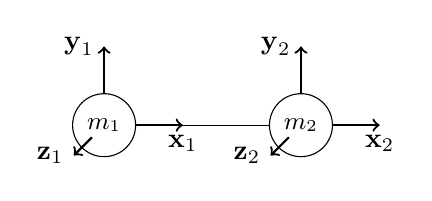
\begin{tikzpicture}
            \draw (2.5,0,0)--(5,0,0);
            \foreach \i in {1,2}{
                \draw[fill=white] (2.5*\i,0,0) node{\small\(m_{\i}\)} circle (0.4);
                \draw[thick,->] (2.5*\i+0.4,0,0)--(2.5*\i+1,0,0)node[below]{\(\vb{x}_{\i}\)};
                \draw[thick,->] (2.5*\i,0.4,0)--(2.5*\i,1,0)node[left]{\(\vb{y}_{\i}\)};
                \draw[thick,->] (2.5*\i,0,0.4)--(2.5*\i,0,1)node[left]{\(\vb{z}_{\i}\)};
            }
        \end{tikzpicture}
        \caption{A basis set representing the motion of a diatomic molecule.}
    \end{figure}

    The simplest model for the internuclear potential is the harmonic oscillator, with the potential given by
    \begin{equation}
        V_{\text{HO}}=\frac{1}{2}k(x_1-x_2)^2\,,
    \end{equation}
    where \(k\) is the force constant. We can write the Hamiltonian as\footnote{We treat this problem using Hamiltonian. If you do Part IB Mathematics, you will solve this type of problems using Lagrangian --- you will find that these two methods are closely related.}
    \begin{equation}
        \hat{H}(\vb{x})=-\frac{\hbar^2}{2m_1}\pdv[2]{}{x_1}-\frac{\hbar^2}{2m_2}\pdv[2]{}{x_2}+\frac{1}{2}k(x_1-x_2)^2\,,
    \end{equation}
    where the first two terms are the kinetic energies of the two particles with masses of \(m_1\) and \(m_2\) respectively. Now this is a non-separable Hamiltonian --- we have cross terms \(x_1x_2\) in the potential energy, so that we cannot write the Hamiltonian as \(\hat{H}(x_1)+\hat{H}(x_2)\). We would not like to solve this kind of partial differential equation directly.

    To make progress, we want to try some coordinate transformation that would make the cross terms vanish. The transformation
    \begin{equation}
        \begin{aligned}
            w_1&=\frac{1}{\sqrt{2}}(x_1-x_2)\\
            w_2&=\frac{1}{\sqrt{2}}(x_1+x_2)
        \end{aligned}
    \end{equation}
    of the components seems promising, since it eliminates the cross terms in the potential energy by making it into a single term \(kw_1^2\). Moreover, these two coordinates have solid physical meaning --- \(w_1\) is the compression/extension along the internuclear axis, which is exactly the vibrational motion we are trying to model, and \(w_2\) describes the translation along the internuclear axis, another motion of the molecule. This is described by the unitary transformation matrix
    \begin{equation}
        \mathsf{U}=\frac{1}{\sqrt{2}}\begin{pmatrix}
            1 & -1 \\
            1 & 1
        \end{pmatrix}
    \end{equation}
    generated by placing the expressions for the new components in terms of the old ones as rows of \(\mathsf{U}\),\footnote{Then the basis vector would transform as \(\mathsf{U}^\dagger\). Remember that the basis vectors and the components transform in the inverse way.} so that the components transform as desired:
    \begin{equation}
        \begin{pmatrix}
            w_1 \\ w_2
        \end{pmatrix}=\mathsf{U}\begin{pmatrix}
            x_1 \\ x_2
        \end{pmatrix}=\frac{1}{\sqrt{2}}\begin{pmatrix}
            1 & -1 \\
            1 & 1
        \end{pmatrix}\begin{pmatrix}
            x_1 \\ x_2
        \end{pmatrix}\,,
    \end{equation}
    or
    \begin{equation}
        \vb{w}=\mathsf{U}\vb{x}\,.
    \end{equation}
    We can be satisfied that no physical properties will be altered by this unitary transformation.

    However, we will see that the problem of this basis transformation is that although the potential terms are nicely simplified, the kinetic term is screwed up. From chain rule, we have
    \begin{align}
        \pdv{}{x_1}&=\pdv{w_1}{x_1}\pdv{}{w_1}+\pdv{w_2}{x_1}\pdv{}{w_2}\notag\\
        &=\frac{1}{\sqrt{2}}\left(\pdv{}{w_1}+\pdv{}{w_2}\right)\,,\\
        \pdv{}{x_2}&=\pdv{w_1}{x_2}\pdv{}{w_1}+\pdv{w_2}{x_2}\pdv{}{w_2}\notag\\
        &=\frac{1}{\sqrt{2}}\left(-\pdv{}{w_1}+\pdv{}{w_2}\right)\,.
    \end{align}
    Therefore in this transformed basis, the Hamiltonian is
    \begin{equation}
        \hat{H}(\vb{w})=-\frac{\hbar^2}{4m_1}\left(\pdv{}{w_1}+\pdv{}{w_2}\right)^2-\frac{\hbar^2}{4m_2}\left(-\pdv{}{w_1}+\pdv{}{w_2}\right)^2+kw_1^2\,.
    \end{equation}
    The kinetic part contains a mixed partial derivative
    \begin{equation}
        -\frac{\hbar^2}{2}\left(\frac{1}{m_1}-\frac{1}{m_2}\right)\pdv{{}^2}{w_1\partial w_2}\,,
    \end{equation}
    which is non-vanishing for \(m_1\ne m_2\).

    It seems that by doing a unitary transformation, we can only separate one of the kinetic and the potential part. Whenever we separate one of the terms, the other will necessarily be screwed up.

    However, the above trial did provide us some inspiration. The mixed partial derivative term does vanish if the masses of the two particles are equal. What if we do some scaling to the coordinates based on the masses? It turns out that for this particular question, the useful scaling is
    \begin{align}
        Q_1&=\sqrt{\frac{m_1m_2}{m_1+m_2}}(x_1-x_2)\\
        Q_2&=\frac{1}{\sqrt{m_1+m_2}}(m_1x_1+m_2x_2)
    \end{align}
    We will explain how we obtained this later, but now let's try this out. Again, the potential is straightforward to rewrite in the \(\vb{Q}\) basis, as
    \begin{equation}
        V_{\text{HO}}=\frac{k(m_1+m_2)}{2m_1m_2}Q_1^2\,.
    \end{equation}
    For the kinetic energies, we again need the chain rule, and we obtain
    \begin{align}
        \pdv{}{x_1}&=\frac{1}{\sqrt{m_1+m_2}}\left(\sqrt{m_1m_2}\pdv{}{Q_1}+m_1\pdv{}{Q_2}\right)\,,\\
        \pdv{}{x_2}&=\frac{1}{\sqrt{m_1+m_2}}\left(-\sqrt{m_1m_2}\pdv{}{Q_1}+m_2\pdv{}{Q_2}\right)\,.
    \end{align}
    If we substitute this into the expression of the Hamiltonian, we will see that all the mixed derivatives magically cancel out and we get
    \begin{equation}
        \hat{H}(Q)=-\frac{\hbar^2}{2}\pdv[2]{}{Q_1}+\frac{k(m_1+m_2)}{2m_1m_2}Q_1^2-\frac{\hbar^2}{2}\pdv[2]{}{Q_2}\,.
    \end{equation}
    This can be nicely separated into
    \begin{equation}
        \hat{H}(\vb{Q})=\hat{H}(Q_1)+\hat{H}(Q_2)\,,
    \end{equation}
    where
    \begin{align}
        \hat{H}(Q_1)&=-\frac{\hbar^2}{2}\pdv[2]{}{Q_1}+\frac{k(m_1+m_2)}{2m_1m_2}Q_1^2\,,\label{diatomic_vib_Hamiltonian}\\
        \hat{H}(Q_2)&=-\frac{\hbar^2}{2}\pdv[2]{}{Q_2}\,.\label{diatomic_trans_Hamiltonian}
    \end{align}
    If we compare (\ref{diatomic_vib_Hamiltonian}) with the Hamiltonian of a canonical harmonic oscillator, we see that this is a harmonic oscillator with a unit mass and a modified force constant of
    \begin{equation}
        k'=\frac{k(m_1+m_2)}{m_1m_2}\eqqcolon\frac{k}{\mu}\,,
    \end{equation}
    where we defined the familiar reduced mass \(\mu\coloneqq m_1m_2/(m_1+m_2)\). This gives an angular frequency
    \begin{equation}
        \omega=\sqrt{\frac{k'}{1}}=\sqrt{\frac{k}{\mu}}\,.
    \end{equation}
    This is a familiar result. The vibration of a diatomic molecule is the same as the vibration of a single molecule with reduced mass of the system. The second equation (\ref{diatomic_trans_Hamiltonian}) has only a kinetic term. This is the translation of the whole molecule along the internuclear axis --- it can also be thought of as a harmonic oscillator with zero force constant, and so a zero frequency.

    \subsubsection{Mass-Weighted Coordinates}
    Now let's consider what is going on. The transformation we proposed can be expressed by the matrix
    \begin{equation}
        \mathsf{A}=\frac{1}{\sqrt{m_1+m_2}}\begin{pmatrix}
            \sqrt{m_1m_2} & -\sqrt{m_1m_2} \\
            m_1 & m_2
        \end{pmatrix}\,.
    \end{equation}
    You may verify that this is not a unitary matrix --- the easiest way to see this is by checking its determinant. Therefore, physical observables do not have to be preserved by this transformation. For example, we can see that all masses have reduced to 1, and the actual masses have somehow been taken into the modified force constant. However, the observable we really care about, the (angular) frequency of the oscillator \(\omega\), is related to the ratio of these, and this is unchanged by our transformation.

    To see what is really going on in our transformation, we can split our transformation into two phases. The first phase is to mass-weight the coordinates, defining \(q_i=\sqrt{m_i}x_i\), which is a diagonal transform, but is not unitary. This is represented by the diagonal matrix
    \begin{equation}
        \mathsf{B}=\begin{pmatrix}
            \sqrt{m_1} & 0 \\
            0 & \sqrt{m_2}
        \end{pmatrix}\,.
    \end{equation}
    The Hamiltonian in this mass-weighted basis set is
    \begin{equation}
        \hat{H}(\vb{q})=-\frac{\hbar^2}{2}\left(\pdv[2]{}{q_1}+\pdv[2]{}{q_2}\right)+\frac{k}{2}\left(\frac{q_1}{\sqrt{m_1}}-\frac{q_2}{\sqrt{m_2}}\right)^2\,.
    \end{equation}
    This transformation does not remove the cross term in the potential, but it has reduced all the kinetic terms to a nice and simple form where all the masses are unity. This is exactly the case that we wanted before --- if the masses are equal, then when you do the unitary transformation to simplify the potential term, all the cross terms in the kinetic term after the transformation will automatically cancel out! We are then ready to do our second transformation defined by
    \begin{align}
        Q_1&=\frac{1}{\sqrt{m_1+m_2}}(\sqrt{m_2}q_1-\sqrt{m_1}q_2)\,,\\
        Q_2&=\frac{1}{\sqrt{m_1+m_2}}(\sqrt{m_1}q_1+\sqrt{m_2}q_2)\,,
    \end{align}
    which can be represented by the unitary matrix
    \begin{equation}
        \mathsf{C}=\frac{1}{\sqrt{m_1+m_2}}\begin{pmatrix}
            \sqrt{m_2} & -\sqrt{m_1}\\
            \sqrt{m_1} & \sqrt{m_2}
        \end{pmatrix}\,.
    \end{equation}
    The combination of these two transformations is the one we claimed before:
    \begin{equation}
        \mathsf{A}=\mathsf{CB}\,.
    \end{equation}
    \subsection{Quadratic Form}
    Before investigating more complicated cases, you may find it extremely useful to formulate the above process in matrices. Hence, we may rewrite the Hamiltonian in the following matrix form
    \begin{align}
        \hat{H}(\vb{x})&=-\frac{\hbar^2}{2}\begin{pmatrix}
            \pdv{}{x_1} & \pdv{}{x_2}
        \end{pmatrix}\begin{pmatrix}
            \frac{1}{m_1} & 0 \\
            0 & \frac{1}{m_2}
        \end{pmatrix}\begin{pmatrix}
            \pdv{}{x_1} \\ \pdv{}{x_2}
        \end{pmatrix}+\frac{1}{2}\begin{pmatrix}
            x_1 & x_2
        \end{pmatrix}\begin{pmatrix}
            k & -k \\
            -k & k
        \end{pmatrix}\begin{pmatrix}
            x_1 \\ x_2
        \end{pmatrix}\notag\\
        &\eqqcolon -\frac{\hbar^2}{2}\vb{\dot{x}}\tp\mathsf{T}_x\vb{\dot{x}}+\frac{1}{2}\vb{x}\tp\mathsf{H}_x\vb{x}\,.
    \end{align}
    The subscript \(x\) here stands for the \(x\) basis, and \(\mathsf{H}\) is confusingly the canonical notation for the Hessian matrix which unfortunately happens to share its notation with the Hamiltonian. Note that \(\dot{\vb{x}}\) here is the gradient operator, not the time derivative of \(\vb{x}\) (velocity).

    Now we can do the transformations. The first step is to mass-scale the coordinates by
    \begin{equation}
        \vb{q}=\mathsf{B}\vb{x}\,,
    \end{equation}
    where
    \begin{equation}
        \mathsf{B}=\begin{pmatrix}
            \sqrt{m_1} & 0 \\
            0 & \sqrt{m_2}
        \end{pmatrix}\,.
    \end{equation}
    Written in suffix notation, this is \(q_i=B_{ij}x_j\). By chain rule, we have
    \begin{align}
        \pdv{}{x_j}&=\pdv{q_i}{x_j}\pdv{}{q_i}\notag \\
        &=B_{ij}\pdv{}{q_i}\notag \\
        &=(B\tp)_{ji}\pdv{}{q_i}\,,
    \end{align}
    or in matrix form,
    \begin{equation}
        \dot{\vb{x}}=\mathsf{B}\tp\dot{\vb{q}}\,.
    \end{equation}
    This gives
    \begin{equation}
        \vb{\dot{x}}\tp\mathsf{T}_x\vb{\dot{x}}=\vb{\dot{q}}\tp\mathsf{B}\mathsf{T}_x\mathsf{B}\tp\vb{\dot{q}}\eqqcolon\vb{\dot{q}}\tp\mathsf{T}_q\vb{\dot{q}}\,.
    \end{equation}
    This transformation is designed to reduce the \(\mathsf{T}\) matrix to the identity matrix in this basis:
    \begin{equation}
        \mathsf{T}_q\coloneqq\mathsf{B}\mathsf{T}_x\mathsf{B}\tp=\mathsf{I}\,,
    \end{equation}
    and so
    \begin{equation}
        \vb{\dot{x}}\tp\mathsf{T}_x\vb{\dot{x}}=\vb{\dot{q}}\tp\mathsf{I}\vb{\dot{q}}=\vb{\dot{q}}\tp\vb{\dot{q}}\,.
    \end{equation}
    Similarly for the Hessian matrix,
    \begin{equation}
        \vb{x}\tp\mathsf{H}_x\vb{x}=\vb{q}\tp(\mathsf{B}^{-1})\tp\mathsf{H}_x\mathsf{B}^{-1}\vb{q}\eqqcolon\vb{q}\tp\mathsf{K}\vb{q}\,,
    \end{equation}
    where the Hessian matrix in this mass-scaled coordinate is called the \textit{dynamical matrix} and is given the special notation \(\mathsf{K}\). We can calculate this as
    \begin{equation}
        \mathsf{K}\coloneqq (\mathsf{B}^{-1})\tp\mathsf{H}_x\mathsf{B}^{-1}=\begin{pmatrix}
            \frac{k}{m_1} & -\frac{k}{\sqrt{m_1m_2}} \\
            -\frac{k}{\sqrt{m_1m_2}} & \frac{k}{m_2}
        \end{pmatrix}\,.
    \end{equation}

    Similarly, we then do the unitary transformation that diagonalises \(\mathsf{K}\) as well, and we finally get
    \begin{equation}
        \mathsf{T}_Q=\mathsf{I}\,,\ \mathsf{H}_Q=\begin{pmatrix}
            0 & 0 \\ 0 & \frac{k}{\mu}
        \end{pmatrix}
    \end{equation}
    in the \(\vb{Q}\) basis. Since both matrices are diagonal, we are then able to separate the Hamiltonian.

    \subsection{The General Case}
    Now we are ready to generalise the above method for all molecules. Consider a molecule consisting of \(N\) atoms. The position of each atom is described by a displacement vector \((x_i,y_i,z_i)\) (\(1\le i\le N\)) from its equilibrium position. We can compactly string them together as a \(3N\)-dimensional vector
    \begin{equation}
        \vb{x}=(x_1,y_1,z_1,\dots,x_N,y_N,z_N)\,.
    \end{equation}
    A general Hamiltonian can be written as
    \begin{equation}
        \hat{H}=-\frac{\hbar^2}{2}\sum_i^{3N}\frac{1}{m_i}\pdv[2]{}{x_i}+\frac{1}{2}\sum_i^{3N}\sum_{j>i}k_{ij}(x_i-x_j)^2\,.
    \end{equation}
    Note that we sum over \(i>j\) in the potential term to avoid double counting, and we allow a potential term to arise between any two coordinates, although in practice we can set most of them to be zero. We can write this into the matrix form introduced above
    \begin{equation}
        \hat{H}=-\frac{\hbar^2}{2}\vb{\dot{x}}\tp\mathsf{T}_x\vb{\dot{x}}+\frac{1}{2}\vb{x}\tp\mathsf{H}_x\vb{x}\,,
    \end{equation}
    where \(\mathsf{T}\) is a diagonal matrix whose elements are the reciprocal masses
    \begin{equation}
        T_{x,ii}=\frac{1}{m_i}\,,
    \end{equation}
    and the Hessian matrix elements are
    \begin{equation}
        H_{x,ij}=\frac{\partial^2 V}{\partial x_i\partial x_j}=\begin{cases}
            \sum_n k_{in} & \text{if }i=j \\
            -k_{ij} & \text{if }i\ne j
        \end{cases}\,.
    \end{equation}

    We first scale the Hamiltonian into the mass-weighted basis \(q_i=\sqrt{m_i}x_i\) so that
    \begin{equation}
        \hat{H}(\vb{q})=-\frac{\hbar^2}{2}\dot{\vb{q}}\tp\dot{\vb{q}}+\frac{1}{2}\vb{q}\tp\mathsf{K}\vb{q}\,.
    \end{equation}
    The matrix \(\mathsf{T}_q\) in the mass-weighted basis is the identity matrix so we have omitted it, and the dynamical matrix is simply
    \begin{equation}
        K_{ij}=\frac{1}{\sqrt{m_im_j}}H_{x,ij}\,.
    \end{equation}
    We now need to transform the basis such that the \(\mathsf{K}\) is made diagonal. We can always do this because \(\mathsf{K}\) is a real symmetric matrix, which is always diagonalisable by an orthogonal matrix (a real unitary matrix). This transformation is guaranteed to keep \(\mathsf{T}\) matrix still diagonalised because the identity matrix is always the identity matrix in any basis. This is done by the orthogonal matrix \(\mathsf{C}\) such that
    \begin{equation}
        \mathsf{H}_Q=\mathsf{C}^\dagger\mathsf{K}\mathsf{C}\,,
    \end{equation} 
    where each column of \(\mathsf{C}\) is the normalised eigenvector of \(\mathsf{K}\), and \(\mathsf{H}_Q\) is a diagonal matrix whose elements are eigenvalues \(\{\lambda_i\}\) of \(\mathsf{K}\) in corresponding order. Finally in this basis, we have
    \begin{align}
        \hat{H}(\vb{Q})&=-\frac{\hbar^2}{2}\dot{\vb{Q}}\tp\dot{\vb{Q}}+\frac{1}{2}\vb{Q}\tp\mathsf{H}_Q\vb{Q}\notag\\
        &=\sum_{i}^{3N}\left(-\frac{\hbar^2}{2}\pdv[2]{}{Q_i}+\frac{1}{2}\lambda_i Q_i^2\right)\label{separated_harmonic_oscillators}
    \end{align}
    separated into \(3N\) one-dimensional harmonic oscillators with modified force constants \(\{\lambda_i\}\). The angular frequencies of the modes are therefore
    \begin{equation}
        \omega_i=\sqrt{\lambda_i}\,.
    \end{equation}
    The eigenvectors of \(\mathsf{K}\), which we denote by \(\vb{e}^{(k)}\), are the displacement vectors of the normal modes in the \(\vb{q}\) basis. Defining the diagonal matrix of masses as \(\mathsf{M}\), so that \(M_{ij}=\delta_{ij}m_i\), we can transform this into the physical \(\vb{x}\) basis via
    \begin{equation}
        \vb{u}^{(k)}=\mathrm{M}^{-1/2}\vb{e}^{(k)}\,,
    \end{equation}
    or in component form
    \begin{equation}
        (\vb{u}^{(k)})_i = \frac{1}{\sqrt{m_i}}(\vb{e}^{(k)})_i\,.
    \end{equation}
    Note that although the normal mode vectors are orthogonal in the \(\vb{q}\) coordinates, they are not necessarily so in the \(\vb{x}\) coordinates since the mass scaling is not unitary. However, we may still often find them to be orthogonal, as they must be so if they transform according to different irreducible representations.

    Note that since we used all \(3N\) displacement vectors, there will be 6 (or 5) normal modes corresponding to translations or rotations. If we use a restricted basis set, there may be less of them. They can be easily identified as modes with frequencies zero.

    The coordinates \(Q_k\) in which the Hamiltonians are nicely separated are called the \textit{normal coordinates}. They are the projections of atomic displacements onto the eigenvectors:
    \begin{equation}
        Q_k=(\vb{e}^{(k)})\tp \vb{q} = (\vb{u}^{(k)})\tp \mathsf{M} \vb{x}\,,
    \end{equation}
    or
    \begin{equation}
        Q_k = \sum_i (\vb{e}^{(k)})_i q_i = \sum_i m_i (\vb{u}^{(k)})_i x_i\,.
    \end{equation}

    \subsection{Example: AAA Linear Molecule}
    As a simple example, let's look at the AAA linear molecule of three identical atoms connected by two bonds of equal strength. An example of this would be the azide anion. For simplicity, we only consider the motions along the internuclear axis.

    \begin{figure}[ht!]
        \centering
        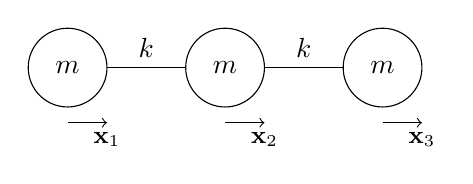
\begin{tikzpicture}
            \draw (-2,0)--(2,0);
            \foreach \i in {1,2,3}{
                \draw[fill=white] (2*\i-4,0) node{\(m\)} circle (0.5);
                \draw[->] (2*\i-4,-0.7)--(2*\i-3.5,-0.7)node[below]{\small\(\vb{x}_{\i}\)};
            }
            \node at (-1,0)[above]{\(k\)};
            \node at (1,0)[above]{\(k\)};
        \end{tikzpicture}
        \caption{An AAA molecule.}
    \end{figure}

    The potential can be modelled as
    \begin{equation}
        V=\frac{k}{2}(x_1-x_2)^2+\frac{k}{2}(x_2-x_3)^2\,.
    \end{equation}
    The Hessian matrix can be found by either taking the partial derivative or by expanding the above function.
    \begin{equation}
        \mathsf{H}_x=\begin{pmatrix}
            k & -k & 0 \\
            -k & 2k & -k \\
            0 & -k & k
        \end{pmatrix}\,.
    \end{equation}
    The dynamical matrix is
    \begin{equation}
        \mathsf{K}=\begin{pmatrix}
            \frac{k}{m} & -\frac{k}{m} & 0 \\
            -\frac{k}{m} & \frac{2k}{m} & -\frac{k}{m} \\
            0 & -\frac{k}{m} & \frac{k}{m}
        \end{pmatrix}\,.
    \end{equation}
    We then simply need to diagonalise this matrix. The eigenvalues and the corresponding normal mode frequencies are
    \begin{align}
        \lambda_1&=0 & \lambda_2&=\frac{k}{m} & \lambda_3&=\frac{3k}{m} \\
        \omega_1&=0 & \omega_2&=\sqrt{\frac{k}{m}} & \omega_3&=\sqrt{\frac{3k}{m}}\,.
    \end{align}
    We can also find the normalised eigenvectors, which give the displacement vectors in the \(\vb{q}\) basis (which is also the normal mode in the \(\vb{x}\) basis since all atoms have equal masses)
    \begin{align}
        \vb{e}_1&=\frac{1}{\sqrt{3}}\begin{pmatrix}
            1 \\ 1 \\ 1
        \end{pmatrix} & \vb{e}_2&=\frac{1}{\sqrt{2}}\begin{pmatrix}
            -1 \\ 0 \\ 1
        \end{pmatrix} & \vb{e}_3&=\frac{1}{\sqrt{6}}\begin{pmatrix}
            1 \\ -2 \\ 1
        \end{pmatrix}\,.
    \end{align}
    In mode 1, all atoms move in the same direction with the same magnitude. This is the translation. Mode 2 is the symmetric stretch, in which both bonds are simultaneously stretched/compressed, and mode 3 is the antisymmetric stretch, in which when one bond is stretched, the other is compressed.
    \begin{figure}[ht!]
        \centering
        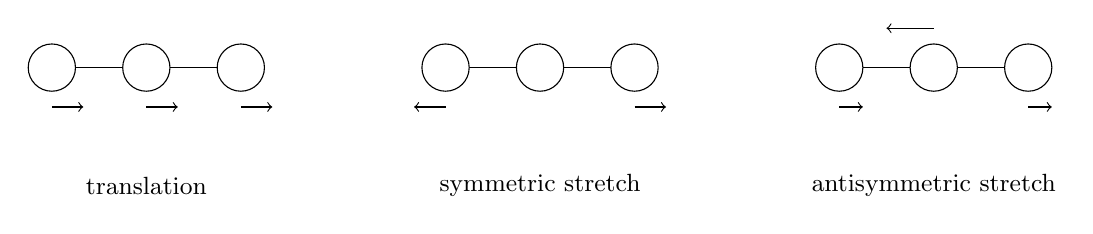
\begin{tikzpicture}
            \begin{scope}[shift={(-5,0)}]
                \draw (-1.2,0)--(1.2,0);
                \foreach \i in {-1,0,1}{
                    \draw[fill=white] (1.2*\i,0) circle (0.3);
                    \draw[->] (1.2*\i,-0.5)--(1.2*\i+0.4,-0.5);
                }
                \node at (0,-1.5){\small translation};
            \end{scope}
            \begin{scope}[shift={(0,0)}]
                \draw (-1.2,0)--(1.2,0);
                \foreach \i in {-1,0,1}{
                    \draw[fill=white] (1.2*\i,0) circle (0.3);
                }
                \draw[->] (-1.2,-0.5)--(-1.6,-0.5);
                \draw[->] (1.2,-0.5)--(1.6,-0.5);
                \node at (0,-1.5){\small symmetric stretch};
            \end{scope}
            \begin{scope}[shift={(5,0)}]
                \draw (-1.2,0)--(1.2,0);
                \foreach \i in {-1,0,1}{
                    \draw[fill=white] (1.2*\i,0) circle (0.3);
                }
                \draw[->] (-1.2,-0.5)--(-0.9,-0.5);
                \draw[->] (1.2,-0.5)--(1.5,-0.5);
                \draw[->] (0,0.5)--(-0.6,0.5);
                \node at (0,-1.5){\small antisymmetric stretch};
            \end{scope}
        \end{tikzpicture}
        \caption{Normal modes of an AAA molecule.}
    \end{figure}

    \subsection{The Use of Symmetry}
    The dynamical matrix in the above example is \(3\times 3\), which we can easily diagonalise directly. For larger molecules, we will encounter the same issue that we had when constructing MOs: any bigger matrix will be too tedious to diagonalise directly by hand. The solution is the same too: we can use an intermediate symmetry-adapted basis set to transform the dynamical matrix to a block-diagonal form.

    We will summarise the process of constructing normal modes by symmetry as well as molecular orbitals in the table below.
    \begin{table}[ht!]
        \centering
        \begin{tabular}{p{7cm}p{7cm}}
            \toprule
            MOs & Normal modes \\ \midrule
            \begin{enumerate}[topsep=0pt]
                \item Write down the Hamiltonian matrix in the AO basis.
                \item Determine the IRs spanned by the AO basis set.
                \item Construct symmetry-adapted combinations of the AOs.
                \item Transform the Hamiltonian matrix into the symmetry-adapted basis set.
                \item The eigenvalues are the orbital energies and the eigenvectors are the MO coefficients in the symmetry-adapted basis set.
                \item The eigenvectors can be transformed back to the AO basis set.
            \end{enumerate}
            &
            \begin{enumerate}[topsep=0pt]
                \item Write down the dynamical matrix in the mass-weighted basis.
                \item Determine IRs spanned by the mass-weighted basis set.
                \item Construct symmetry-adapted combinations of the mass-weighted coordinates.
                \item Transform the dynamical matrix into the symmetry-adapted basis set.
                \item The eigenvalues are the frequencies squared and the eigenvectors are the normal mode coordinates in the symmetry-adapted basis set.
                \item The eigenvectors can be transformed back to the coordinate displacement basis set.
            \end{enumerate} \\ \bottomrule
        \end{tabular}
    \end{table}

    \subsection{Example: \texorpdfstring{\reflectbox{BA}BA}{ABBA} Linear Molecule}
    Consider the motions along the bond for a centrosymmetric \reflectbox{BA}BA linear molecule, for example acetylene. The masses of the two types of atoms are now different, and we also allow the strength of the \(\mathrm{A-B}\) bond to be different from the \(\mathrm{B-B}\) bond.
    \begin{figure}[ht!]
        \centering
        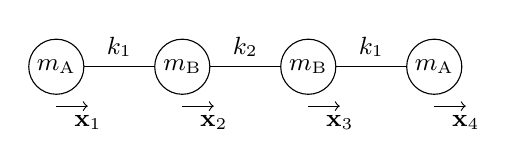
\begin{tikzpicture}
            \draw (-2.4,0)--(2.4,0);
            \foreach \i in {1,-1}{
                \draw[fill=white] (0.8*\i,0) node{\small\(m_{\BB}\)} circle (0.35);
                \draw[fill=white] (2.4*\i,0) node{\small\(m_{\AA}\)} circle (0.35);
                \node at (1.6*\i,0)[above]{\small\(k_1\)};
            }
            \node at (0,0)[above]{\small\(k_2\)};
            \foreach \i in {1,2,3,4}{
                \draw[->] (1.6*\i-4,-0.5)--(1.6*\i-3.6,-0.5)node[below]{\small\(\vb{x}_{\i}\)};
            }
        \end{tikzpicture}
        \caption{A centrosymmetric \reflectbox{BA}BA linear molecule.}
    \end{figure}

    If we proceed without using symmetry, then we have a \(4\times 4\) dynamical matrix to diagonalise
    \begin{equation}
        \mathsf{K}=\begin{pmatrix}
            \frac{k_1}{m_{\AA}} & -\frac{k_1}{\sqrt{m_{\AA}m_{\BB}}} & 0 & 0 \\
            -\frac{k_1}{\sqrt{m_{\AA}m_{\BB}}} & \frac{k_1+k_2}{m_{\BB}} & -\frac{k_2}{m_{\BB}} & 0 \\
            0 & -\frac{k_2}{m_{\BB}} & \frac{k_1+k_2}{m_{\BB}} & -\frac{k_1}{\sqrt{m_{\AA}m_{\BB}}} \\
            0 & 0 & -\frac{k_1}{\sqrt{m_{\AA}m_{\BB}}} & \frac{k_1}{m_{\AA}}
        \end{pmatrix}\,.
    \end{equation}
    To simplify things up, we will create a \(\tilde{\vb{q}}\) basis from symmetry-adapted combinations of \(\vb{q}\). The point group of the molecule is \(D_{\infty h}\), and we can split the basis into two two-dimensional sets \(\{\vb{q}_1,\vb{q}_4\}\) and \(\{\vb{q}_2,\vb{q}_3\}\). The irreducible representations and the symmetry-adapted combinations of basis vectors should be easy to find\footnote{Recall when constructing a representation, we transform the basis, not the components.}
    \begin{align}
        \tilde{\vb{q}}_1&=\frac{1}{\sqrt{2}}(\vb{q}_1-\vb{q}_4) & &\Sigma_g^+ \\
        \tilde{\vb{q}}_2&=\frac{1}{\sqrt{2}}(\vb{q}_2-\vb{q}_3) & &\Sigma_g^+ \\
        \tilde{\vb{q}}_3&=\frac{1}{\sqrt{2}}(\vb{q}_1+\vb{q}_4) & &\Sigma_u^+ \\
        \tilde{\vb{q}}_4&=\frac{1}{\sqrt{2}}(\vb{q}_2+\vb{q}_3) & &\Sigma_u^+ \,.
    \end{align}
    This is the basis transformation represented by the unitary matrix
    \begin{equation}
        \tilde{\mathsf{C}}=\frac{1}{\sqrt{2}}\begin{pmatrix}
            1 & 0 & 1 & 0 \\
            0 & 1 & 0 & 1 \\
            0 & -1 & 0 & 1 \\
            -1 & 0 & 1 & 0
        \end{pmatrix}
    \end{equation}
    so that the components transform as
    \begin{equation}
        \tilde{\vb{q}}=\tilde{\mathsf{C}}^\dagger\vb{q}\,.
    \end{equation}
    We must have
    \begin{equation}
        \vb{q}^\dagger\mathsf{K}\vb{q}=\tilde{\vb{q}}^\dagger\tilde{\mathsf{K}}\tilde{\vb{q}}=\vb{q}^\dagger\tilde{\mathsf{C}}\tilde{\mathsf{K}}\tilde{\mathsf{C}}^\dagger\vb{q}\,,
    \end{equation}
    and so\footnote{An easier thing to do is to evaluate the matrix component by component, using \(\tilde{K}_{ij}=\tilde{\vb{q}}_i^\dagger \mathsf{K}\tilde{\vb{q}}_j\).}
    \begin{align}
        \tilde{\mathsf{K}}&=\tilde{\mathsf{C}}^\dagger\mathsf{K}\tilde{\mathsf{C}}\notag\\
        &=\begin{pmatrix}
            \frac{k_1}{m_{\AA}} & -\frac{k_1}{\sqrt{m_{\AA}m_{\BB}}} & 0 & 0 \\
            -\frac{k_1}{\sqrt{m_{\AA}m_{\BB}}} & \frac{k_1+2k_2}{m_{\BB}} & 0 & 0 \\
            0 & 0 & \frac{k_1}{m_{\AA}} & -\frac{k_1}{\sqrt{m_{\AA}m_{\BB}}} \\
            0 & 0 & -\frac{k_1}{\sqrt{m_{\AA}m_{\BB}}} & \frac{k_1}{m_{\BB}}
        \end{pmatrix}\,.
    \end{align}
    This is block-diagonal as expected. For simplicity, we will only work out the \(\Sigma_u^+\) (bottom right) block. The eigenvalues are
    \begin{align}
        \lambda_3&=0 & \lambda_4&=\frac{k_1(m_{\AA}+m_{\BB})}{m_{\AA}m_{\BB}}\,,
    \end{align}
    and the eigenvectors in the various basis sets are
    \begin{align}
        \tilde{\vb{e}}_3&=\frac{1}{\sqrt{m_{\AA}+m_{\BB}}}\begin{pmatrix}
            \sqrt{m_{\AA}} \\ \sqrt{m_{\BB}}
        \end{pmatrix}_{\tilde{\vb{q}}_{\Sigma_u^+}} & \tilde{\vb{e}}_4&=\frac{1}{\sqrt{m_{\AA}+m_{\BB}}}\begin{pmatrix}
            \sqrt{m_{\BB}} \\ -\sqrt{m_{\AA}}
        \end{pmatrix}_{\tilde{\vb{q}}_{\Sigma_u^+}} \notag\\
        \vb{e}_3&=\frac{1}{\sqrt{2(m_{\AA}+m_{\BB})}}\begin{pmatrix}
            \sqrt{m_{\AA}} \\ \sqrt{m_{\BB}} \\ \sqrt{m_{\BB}} \\ \sqrt{m_{\AA}}
        \end{pmatrix}_{\vb{q}} & \vb{e}_4&=\frac{1}{\sqrt{2(m_{\AA}+m_{\BB})}}\begin{pmatrix}
            \sqrt{m_{\BB}} \\ -\sqrt{m_{\AA}} \\ -\sqrt{m_{\AA}} \\ \sqrt{m_{\BB}}
        \end{pmatrix}_{\vb{q}} \notag\\
        \vb{u}_3&=\frac{1}{2}\begin{pmatrix}
            1 \\ 1 \\ 1 \\ 1
        \end{pmatrix}_{\vb{x}} & \vb{u}_4&=\frac{\sqrt{m_{\AA}m_{\BB}}}{\sqrt{2(m_{\AA}^2+m_{\BB}^2)}}\begin{pmatrix}
            \sqrt{\frac{m_{\BB}}{m_{\AA}}} \\ -\sqrt{\frac{m_{\AA}}{m_{\BB}}} \\ -\sqrt{\frac{m_{\AA}}{m_{\BB}}} \\ \sqrt{\frac{m_{\BB}}{m_{\AA}}}
        \end{pmatrix}_{\vb{x}}\,.
    \end{align}
    We've added subscripts labelling the basis that the displacement vectors are represented in to avoid confusion.

    Mode three is the uniform translation, and mode four is the antisymmetric stretch in which when one \(\mathrm{A-B}\) bond is stretched, the other is compressed.

    \begin{figure}[ht!]
        \centering
        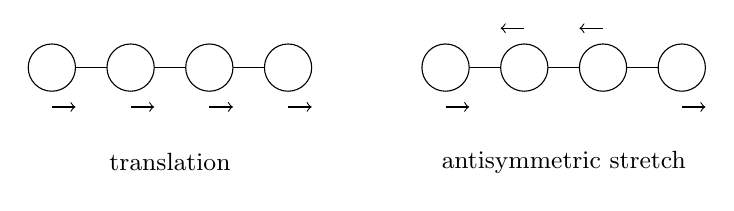
\begin{tikzpicture}
            \draw (-1.5,0)--(1.5,0);
            \foreach \i in {1,...,4}{
                \draw[fill=white] (\i-2.5,0) circle (0.3);
                \draw[->] (\i-2.5,-0.5)--(\i-2.2,-0.5);
            }
            \node at (0,-1.2) {\small translation};

            \begin{scope}[shift={(5,0)}]
                \draw (-1.5,0)--(1.5,0);
                \foreach \i in {1,...,4}{
                    \draw[fill=white] (\i-2.5,0) circle (0.3);
                }
                \draw[->] (-1.5,-0.5)--(-1.2,-0.5);
                \draw[->] (1.5,-0.5)--(1.8,-0.5);
                \draw[->] (-0.5,0.5)--(-0.8,0.5);
                \draw[->] (0.5,0.5)--(0.2,0.5);
                \node at (0,-1.2) {\small antisymmetric stretch};
            \end{scope}
        \end{tikzpicture}
    \end{figure}

    \subsection{Beyond Harmonic Oscillators}
    Real molecules are not harmonic oscillators in general. We will have some complicated potential as a function of the nuclear coordinates, which defines the nuclear \textit{potential energy surface} (PES). We can perform a Taylor expansion around an equilibrium position to get
    \begin{equation}
        V(\vb{R})=V(\vb{R}_{\text{eq}})+\sum_{i=1}^{3N}x_i\pdv{V}{x_i}\bigg|_{\vb{R}_{\text{eq}}}+\frac{1}{2}\sum_{i=1}^{3N}\sum_{j=1}^{3N}x_ix_j\frac{\partial^2 V}{\partial x_i\partial x_j}\bigg|_{\vb{R}_{\text{eq}}}+O(x_ix_jx_k)\,.
    \end{equation}
    \(V(\vb{R}_{\text{eq}})\) is the energy at the bottom of the potential well, which we can set to 0, and the first derivatives at the equilibrium positions should also be 0. For sufficiently small oscillations, the cubic terms and above are not significant, so we can truncate our expression at the quadratic term, which is equivalent to making a harmonic approximation. We are left with
    \begin{equation}\label{harmonic_approximation}
        V(\vb{R})\approx\frac{1}{2}\sum_{i,j=1}^{3N}x_ix_j\frac{\partial^2 V}{\partial x_i\partial x_j}\bigg|_{\vb{R}_{\text{eq}}}=\frac{1}{2}\vb{x}\tp\mathsf{H}_x\vb{x}
    \end{equation}
    with Hessian matrix elements
    \begin{equation}
        \mathsf{H}_{x,ij}=\frac{\partial^2 V}{\partial x_i\partial x_j}\bigg|_{\vb{R}_{\text{eq}}}\,.
    \end{equation}
    For harmonic potentials, this is equivalent to finding the quadratic coefficients of \(V\). If we want to include the effect of cubic terms and above, we can do this by perturbation theory, which is the topic of the rest of this course.

    \subsection{Transition States}
    The eigenvalues of the Hessian matrix represent the second derivatives of the potential energies along the principal directions. Recall that a positive second derivative corresponds to a minimum. Ignoring the six directions that do not correspond to an internal change of the molecule, we can classify a stationary point on the potential energy surface according to the number of negative Hessian eigenvalues. If there are no negative Hessian eigenvalues, then this is a minimum on the PES. If all the eigenvalues are negative, the point is a maximum.

    The Murrell--Laidler definition of a \textit{transition state} is an index-1 saddle point, that is a stationary point with only one negative Hessian value. Therefore a transition state is a maximum along one direction and a minimum in all other orthogonal directions. The normal mode corresponding to the negative Hessian eigenvalue is the reaction coordinate at the transition state. Since the vibrational frequency is the square root of the eigenvalue, the frequency in such a direction is imaginary.\footnote{This statement should make you question the derivation of transition state theory presented in the Part IB MELT course. A rigorous treatment of reaction kinetics will be left to Part III.}

    \newpage

    \section{Non-Degenerate Perturbation Theory}
    \subsection{Non-Degenerate Perturbation Theory}
    Often the Schr\"{o}dinger equation of a Hamiltonian \(\hat{H}\) will be too complicated to be solved directly:
    \begin{equation}\label{Schrodinger_eqn}
        \hat{H}\psi_n=E_n\psi_n\,,
    \end{equation}
    where \(n\in\NN\) labelling the quantum states. Then we need to start to make approximations. The starting point of the perturbation theory is to find a simpler Hamiltonian, which we call \(\hat{H}^{(0)}\), that somewhat resembles \(H\) but whose eigenfunctions \(\psi_n^{(0)}\) and eigenvalues \(E_n^{(0)}\) are known:
    \begin{equation}\label{unperturbed_Schrodinger}
        \hat{H}^{(0)}\psi_n^{(0)}=E_n^{(0)}\psi_n^{(0)}\,.
    \end{equation}
    At this stage we will assume that the states are non-degenerate.

    The next thing we do is to consider the whole one-parameter family of Hamiltonians
    \begin{equation}
        \hat{H}(\lambda)=\hat{H}^{(0)}+\lambda\hat{H}^{(1)}
    \end{equation}
    such that
    \begin{equation}
        \hat{H}(\lambda^*)=\hat{H}
    \end{equation}
    at some specific value of \(\lambda=\lambda^*\). \(\hat{H}^{(1)}\) is the \textit{perturbation} to the reference Hamiltonian. Usually we would just let
    \begin{equation}
        \hat{H}^{(1)}=\hat{H}-\hat{H}^{(0)}
    \end{equation}
    so that \(\hat{H}(\lambda)\) becomes the Hamiltonian \(\hat{H}\) of interest at \(\lambda=1\). However, sometimes the perturbation to the reference Hamiltonian has a natural perturbation in it. For example, if we consider applying a small electric field \(\mathcal{E}\vu{z}\) to a molecule with dipole \(\vb{\mu}\), then the strength of the electric field \(\mathcal{E}\) will be a natural perturbation parameter.

    Then the fundamental assumption in perturbation theory is to assume that both the energies and the quantum states are analytic near \(\lambda=0\), so that if we gradually turn on the perturbation from the reference state where \(\lambda=0\) to some small non-zero \(\lambda\), the energies and the wavefunctions will also change smoothly given by the power series
    \begin{align}
        \psi_n(\lambda)&=\psi_n^{(0)}+\lambda\psi_n^{(1)}+\lambda^2\psi_n^{(2)}+\dots \label{state_expansion}\\
        E_n(\lambda)&=E_n^{(0)}+\lambda E_n^{(1)}+\lambda^2 E_n^{(2)}+\dots \label{energy_expansion}
    \end{align}
    In the hope that these series do converge to the true values, we can then evaluate these power series expansions (usually the first few correction terms only) at the desired value of \(\lambda\) to get an approximation of the true \(E_n\) and \(\psi_n\).

    \begin{figure}
        \centering
        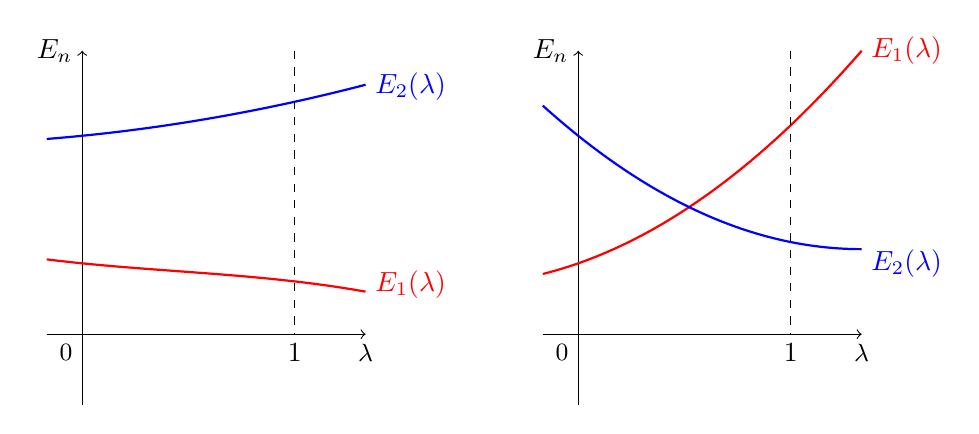
\begin{tikzpicture}[scale=0.9]
            \draw[->] (-0.5,0)--(4,0)node[below]{\small\(\lambda\)};
            \draw[->] (0,-1)--(0,4)node[left]{\(E_n\)};
            \node at (0,0)[below left]{\small \(0\)};
            \draw[red,thick,domain=-0.5:4, smooth, variable=\x,samples=50] plot ({\x}, {1-0.1*\x+0.02*\x*\x-0.005*\x*\x*\x});
            \node[red] at (4,0.7)[right]{\(E_1(\lambda)\)};
            \draw[blue,thick,domain=-0.5:4, smooth, variable=\x,samples=50] plot ({\x}, {2.8+0.1*\x+0.02*\x*\x});
            \node[blue] at (4,3.5)[right]{\(E_2(\lambda)\)};
            \draw[dashed] (3,4)--(3,0)node[below]{\(1\)};

            \begin{scope}[shift={(7,0)}]
                \draw[->] (-0.5,0)--(4,0)node[below]{\small\(\lambda\)};
                \draw[->] (0,-1)--(0,4)node[left]{\(E_n\)};
                \node at (0,0)[below left]{\small \(0\)};
                \draw[red,thick,domain=-0.5:4, smooth, variable=\x,samples=50] plot ({\x}, {1+0.35*\x+0.1*\x*\x});
                \node[red] at (4,4)[right]{\(E_1(\lambda)\)};
                \draw[blue,thick,domain=-0.5:4, smooth, variable=\x,samples=50] plot ({\x}, {2.8-0.8*\x+0.1*\x*\x});
                \node[blue] at (4,1)[right]{\(E_2(\lambda)\)};
                \draw[dashed] (3,4)--(3,0)node[below]{\(1\)};
            \end{scope}
        \end{tikzpicture}
        \caption{The perturbation theory is appropriate in the first case, in which the reference Hamiltonian is ``close enough'' to the true Hamiltonian such that the perturbation only leads to small changes in the energies and wavefunctions. The perturbation theory may not work in the second case where the changes in energy levels is comparable with the energy level separations. The reference Hamiltonian is too far away from the true Hamiltonian. Either we will then need too many terms in the series expansion to get a satisfactory result, or the series just may not converge. We will discuss this convergence issue in appendix \cref{Appendix:Converge}.}
    \end{figure}

    We will employ the conventional \textit{intermediate normalisation}, where the unperturbed wavefunction will be normalised
    \begin{equation}
        \braket{\psi_n^{(0)}}{\psi_n^{(0)}}\equiv\braket{n}{n}=1\,.
    \end{equation}
    This choice means that the perturbed wavefunctions \(\psi_n(\lambda)\) will not be normalised. However, since \(\psi_n^{(1)},\psi_n^{(2)},\dots\) are corrections to \(\psi_n^{(0)}\), we may require that
    \begin{equation}
        \braket{n}{\psi_n^{(i)}}=0
    \end{equation}
    for all \(i>0\), from which it follows that
    \begin{equation}
        \braket{n}{\psi_n}=1\,.
    \end{equation}
    We can claim this because if \(\psi_n^{(i)}\) has some non-zero \(\psi_n^{(0)}\) component for \(i>0\), we can absorb it into \(\psi_n^{(0)}\) and renormalise \(\psi_n\) to make the coefficient of \(\psi_n^{(0)}\) to be 1 again.

    \subsubsection{The Perturbation Equations}
    To work out the coefficients \(E_n^{(i)}\) and \(\psi_n^{(i)}\) of the power series, we simply need to plug the expansion ansatz (\ref{energy_expansion}) and (\ref{state_expansion}) into the Schr\"{o}dinger equation (\ref{Schrodinger_eqn}) to get
    \begin{equation}\label{perturbed_Schrodinger}
        (\hat{H}^{(0)}+\lambda\hat{H}^{(1)}-E_n^{(0)}-\lambda E_n^{(1)}-\lambda^2 E_n^{(2)}+\dots)(\psi_n^{(0)}+\lambda\psi_n^{(1)}+\lambda^2\psi_n^{(2)}+\dots)=0\,.
    \end{equation}
    For this equation to be satisfied for all \(\lambda\) sufficiently small such that the series converges, the coefficients of all powers of \(\lambda\) must be zero. Gathering the terms in \(\lambda^0\), \(\lambda^1\), \(\lambda^2\),\dots, we get a series of equations
    \begin{align}
        (\hat{H}^{(0)}-E_n^{(0)})\ket{\psi_n^{(0)}}&=0\label{perturbation_eqn_zero}\\
        (\hat{H}^{(0)}-E_n^{(0)})\ket{\psi_n^{(1)}}+(\hat{H}^{(1)}-E_n^{(1)})\ket{\psi_n^{(0)}}&=0\label{perturbation_eqn_first}\\
        (\hat{H}^{(0)}-E_n^{(0)})\ket{\psi_n^{(2)}}+(\hat{H}^{(1)}-E_n^{(1)})\ket{\psi_n^{(1)}}-E_n^{(2)}\ket{\psi_n^{(0)}}&=0\label{perturbation_eqn_second}\\
        \vdots\qquad\qquad&\notag
    \end{align}
    The zeroth-order equation (\ref{perturbation_eqn_zero}) is exactly the unperturbed Schr\"{o}dinger equation (\ref{unperturbed_Schrodinger}), which we should have already solved. The next equation of interest is the first-order equation (\ref{perturbation_eqn_first}). If we contract it with \(\bra{\psi_n^{(0)}}\equiv\bra{n}\), we get
    \begin{equation}
        \mel{n}{\hat{H}^{(0)}-E_n^{(0)}}{\psi_n^{(1)}}+\expval{\hat{H}^{(1)}-E_n^{(1)}}{n}=0\,.
    \end{equation}
    Since \(\hat{H}^{(0)}\) is Hermitian, the first term vanishes:
    \begin{equation}
        \mel{n}{\hat{H}^{(0)}-E_n^{(0)}}{\psi_n^{(1)}}=\mel{\psi_n^{(1)}}{\hat{H}^{(0)}-E_n^{(0)}}{n}^*=0\,,
    \end{equation}
    and we are left with
    \begin{equation}\label{first_order_energy}
        E_n^{(1)}=\expval{\hat{H}^{(1)}}{n}\,.
    \end{equation}
    This is the key result in perturbation theory. The first-order correction in energy is simply the expectation value of the perturbation for the unperturbed state. This also implies that
    \begin{equation}
        E_n^{(0)}+\lambda E_n^{(1)}=\expval{\hat{H}^{(0)}+\lambda\hat{H}^{(1)}}{n}=\expval{\hat{H}}{n}\,.
    \end{equation}
    The energy corrected to first order is the expectation value of the complete Hamiltonian with the unperturbed wavefunction.

    A similar procedure yields the second-order energy. If we contract the second-order perturbation equation (\ref{perturbation_eqn_second}) with \(\bra{n}\), we get
    \begin{equation}
        \mel{n}{\hat{H}^{(0)}-E_n^{(0)}}{\psi_n^{(2)}}+\mel{n}{\hat{H}^{(1)}-E_n^{(1)}}{\psi_n^{(1)}}-\expval{E_n^{(2)}}{n}=0\,.
    \end{equation}
    The first term again vanishes since \(\hat{H}^{(0)}\) is Hermitian. By the intermediate normalisation, we also have \(E_n^{(1)}\braket{n}{\psi_n^{(1)}}\) in the second term vanishes and the third term \(\expval{E_n^{(2)}}{n}=E_n^{(2)}\). Therefore, the second-order energy is
    \begin{equation}\label{second_order_energy}
        E_n^{(2)}=\mel{n}{\hat{H}^{(1)}}{\psi_n^{(1)}}\,.
    \end{equation}
    To use this expression we will need to obtain the first-order wavefunction \(\psi_n^{(1)}\). This can be obtained by solving the complicated first-order equation (\ref{perturbation_eqn_first}), which we don't expect to have a simple closed form solution in general unless in very simple cases. We will introduce alternative methods to work this out later.

    \subsubsection{Higher-order Energies and Wigner's \texorpdfstring{\(2n+1\)}{2n+1} Theorem}
    By expanding higher order terms of (\ref{perturbed_Schrodinger}), one can show that the \(n^{\text{th}}\)-order correction in energy is given by
    \begin{equation}\label{ith_order_energy}
        E_n^{(i)}=\mel{n}{\hat{H}^{(1)}}{\psi_n^{(i-1)}}\,,
    \end{equation}
    so it seems that we need to know the wavefunction to the order \(i-1\) to calculate the energy to order \(i\). In fact, we can do better than this.
    \begin{thm}[Wigner's \(2n+1\) rule]
        The \(2n+1^{\text{st}}\)-order correction to the energy can be calculated from the first \(n^{\text{th}}\)-order perturbation of wavefunctions.
    \end{thm}
    This is more easily seen in a different formulation of the perturbation theory called the \textit{Wigner--Brillouin perturbation theory}, but it is a far more complicated topic. A brief proof of this is in appendix \cref{Appendix:Wigner}, and here we will only show explicitly how to construct \(E_n^{(3)}\) from \(\psi_n^{(1)}\).

    If we contract the first-order perturbation equation (\ref{perturbation_eqn_first}) with the second-order wavefunction \(\bra{\psi_n^{(2)}}\), we get an overall third-order expression
    \begin{equation}
        \mel{\psi_n^{(2)}}{\hat{H}^{(0)}-E_n^{(0)}}{\psi_n^{(1)}}+\mel{\psi_n^{(2)}}{\hat{H}^{(1)}-E_n^{(1)}}{n}=0\,.
    \end{equation}
    By (\ref{ith_order_energy}) and the intermediate normalisation, we identify the second term as \(E_n^{(3)}\), and so
    \begin{equation}\label{Wigner_third_energy}
        E_n^{(3)}=-\mel{\psi_n^{(2)}}{\hat{H}^{(0)}-E_n^{(0)}}{\psi_n^{(1)}}\,.
    \end{equation}
    We can get another third-order expression by contracting the second-order equation (\ref{perturbation_eqn_second}) with the first-order wavefunction \(\bra{\psi_n^{(1)}}\)
    \begin{equation}
        \mel{\psi_n^{(1)}}{\hat{H}^{(0)}-E_n^{(0)}}{\psi_n^{(2)}}+\mel{\psi_n^{(1)}}{\hat{H}^{(1)}-E_n^{(1)}}{\psi_n^{(1)}}=0\,.
    \end{equation}
    We identify the first term in the above expression as the negative third-order energy by (\ref{Wigner_third_energy}), and so
    \begin{equation}
        E_n^{(3)}=\expval{\hat{H}^{(1)}-E_n^{(1)}}{\psi_n^{(1)}}\,,
    \end{equation}
    which contains only the first-order wavefunction as claimed.

    We can obtain higher order expression using the same trick as above, but they will be much more complicated to derive and are rarely needed. For a problem to be properly treated using perturbation theory, the higher order corrections should be small and so the series should converge quickly.

    \subsection{The Hellmann--Feynman Theorem}
    We have formulated the perturbation problem as the eigenvalue problem of a family of one-parameter Hamiltonians
    \begin{equation}
        \hat{H}(\lambda)\psi(\lambda)=E(\lambda)\psi(\lambda)\,.
    \end{equation}
    How the energy \(E(\lambda)\) changes against \(\lambda\) actually tells us something more about the system.

    \begin{thm}[Hellmann--Feynman theorem]
        Let \(E(\lambda)\) and \(\psi(\lambda)\) be the eigenvalues and eigenstates of the one-parameter family of Hamiltonians
        \begin{equation}
            \hat{H}(\lambda)\psi(\lambda)=E(\lambda)\psi(\lambda)\,,
        \end{equation}
        then
        \begin{equation}
            \dv{E(\lambda)}{\lambda}=\expval{\dv{\hat{H}(\lambda)}{\lambda}}{\psi(\lambda)}\,.
        \end{equation}
    \end{thm}
    \begin{proof}
        Let \(\psi(\lambda)\) be normalised. Then by the product rule,
        \begin{align}
            \dv{E(\lambda)}{\lambda}&=\dv{}{\lambda}\expval{\hat{H}(\lambda)}{\psi(\lambda)}\notag \\
            &=\mel{\dv{\psi(\lambda)}{\lambda}}{\hat{H}(\lambda)}{\psi(\lambda)}+\expval{\dv{\hat{H}(\lambda)}{\lambda}}{\psi(\lambda)}+\mel{\psi(\lambda)}{\hat{H}(\lambda)}{\dv{\psi(\lambda)}{\lambda}}\notag\\
            &=\expval{\dv{\hat{H}(\lambda)}{\lambda}}{\psi(\lambda)}+E(\lambda)\left[\braket{\dv{\psi(\lambda)}{\lambda}}{\psi(\lambda)}+\braket{\psi(\lambda)}{\dv{\psi(\lambda)}{\lambda}}\right]\notag \\
            &=\expval{\dv{\hat{H}(\lambda)}{\lambda}}{\psi(\lambda)}+E(\lambda)\dv{}{\lambda}\braket{\psi(\lambda)}{\psi(\lambda)}\notag\\
            &=\expval{\dv{\hat{H}(\lambda)}{\lambda}}{\psi(\lambda)}\,.
        \end{align}\qed
    \end{proof}

    Let's make a connection with the perturbation theory. We can expand \(E(\lambda)\) in a Taylor series
    \begin{equation}
        E(\lambda)=E(0)+\dv{E}{\lambda}\bigg|_{\lambda=0}\lambda+\frac{1}{2}\dv[2]{E}{\lambda}\bigg|_{\lambda=0}\lambda^2+\dots
    \end{equation}
    Then we may identify the \(n^{\text{th}}\) derivatives of \(E(\lambda)\) at \(\lambda=0\) as the \(n^{\text{th}}\)-order correction in energy
    \begin{align}
        E^{(1)}&=\dv{E}{\lambda}\bigg|_{\lambda=0}\\
        E^{(2)}&=\frac{1}{2}\dv[2]{E}{\lambda}\bigg|_{\lambda=0}\\
        &\quad\vdots\notag
    \end{align}

    Now, for example, consider a molecule/atom in an electric field of strength \(\mathcal{E}\) parallel to the \(z\) axis, for which the Hamiltonian is
    \begin{equation}
        \hat{H}(\mathcal{E})=\hat{H}^{(0)}-\mathcal{E}\hat{\mu}_z\,,
    \end{equation} 
    where \(\hat{H}^{(0)}\) is the molecular Hamiltonian without external fields and \(\hat{\mu}_z=\sum_i q_i z_i\) is the \(z\)-component of the dipole moment operator. We have
    \begin{equation}
        \dv{\hat{H}(\mathcal{E})}{\mathcal{E}}=-\hat{\mu}_z\,.
    \end{equation}
    Using the Hellmann--Feynman theorem, we can write
    \begin{equation}
        E^{(1)}=\dv{E}{\mathcal{E}}\bigg|_{\mathcal{E}=0}=-\expval{\hat{\mu}_z}{\psi(\mathcal{E}=0)}\,.
    \end{equation}
    This is the expectation value of the dipole moment in the unperturbed state, which is, by definition, the permanent dipole moment,
    \begin{equation}
        E^{(1)}=-\mu_z^0\,.
    \end{equation}
    Looking at the second-order contribution, we have
    \begin{equation}
        E^{(2)}=\frac{1}{2}\dv[2]{E}{\mathcal{E}}\bigg|_{\mathcal{E}=0}=\frac{1}{2}\dv{}{\mathcal{E}}(-\mu_z)\bigg|_{\mathcal{E}=0}\,.
    \end{equation}
    The definition of the polarisability is exactly
    \begin{equation}
        \alpha_{ij}\coloneqq\dv{\mu_{i}}{\mathcal{E}_j}\bigg|_{\mathcal{E}_j=0}\,,
    \end{equation}
    and so
    \begin{equation}
        E^{(2)}=-\frac{1}{2}\alpha_{zz}\,.
    \end{equation}

    \begin{ex}
        \textit{Quadratic Stark effect and the polarisability of hydrogen atom.}

        Consider the ground electronic state of the hydrogen atom, where the electronic Hamiltonian, ground state wavefunction and energy are
        \begin{align}
            \hat{H}^{(0)}&=-\frac{1}{2}\laplacian-\frac{1}{r}\\
            \psi_0^{(0)}&=\frac{1}{\sqrt{\pi}}\ee^{-r}\\
            E_0^{(0)}&=-\frac{1}{2}\,.
        \end{align}
        We again consider the perturbation of an external electric field of strength \(\mathcal{E}\) in the \(z\) direction, giving a perturbing Hamiltonian
        \begin{align}
            \lambda&=\mathcal{E} & \hat{H}^{(1)}&=z\,.
        \end{align}
        The first-order energy is
        \begin{equation}
            E_0^{(1)}=\expval{z}{0}=0\,,
        \end{equation}
        which can easily be evaluated by symmetry. This shows that a ground state hydrogen atom has no permanent dipole moment. Using the first-order perturbation equation (\ref{perturbation_eqn_first}), one can obtain the differential equation
        \begin{equation}
            \left(-\frac{1}{2}\laplacian-\frac{1}{r}+\frac{1}{2}\right)\psi_0^{(1)}+\frac{1}{\sqrt{\pi}}ze^{-r}=0\,.
        \end{equation}
        This is one of the extremely rare cases where the first-order wavefunction can be solved analytically in a closed form,\footnote{Even in this case, this equation is not easy to solve at all! You need to change to parabolic coordinates and do fancy stuff.} which gives
        \begin{equation}
            \psi_0^{(1)}=-\frac{1}{\sqrt{\pi}}\left(1+\frac{r}{2}\right)ze^{-r}\,.
        \end{equation}
        One can then obtain the exact second-order energy
        \begin{equation}
            E_0^{(2)}=\mel{0}{z}{\psi_0^{(1)}}=-\frac{9}{4}\,.
        \end{equation}
        Hence, the electronic energy of hydrogen in an electric field of strength \(\mathcal{E}\) is given by
        \begin{equation}
            E=-\frac{1}{2}-\frac{9}{4}\mathcal{E}^2+O(\mathcal{E}^4)\,,
        \end{equation}
        where one can actually argue that only even power terms are permitted by symmetry. This tells us that the ground state hydrogen atom has a polarisability of \(\alpha=9/2\) exactly.

        This is a particularly important example, which we will use as a benchmark for the methods introduced later since we know the answer exactly.
    \end{ex}

    \subsection{Matrix Formulation}
    Let's say we have an unperturbed wavefunction expressed in some orthonormal basis \(\{\phi_i\}\)
    \begin{equation}
        \ket{\psi_n^{(0)}}=\sum_i c_{ni}\phi_i=\vb{\phi}\tp\vb{c}_n\,.
    \end{equation}
    Then if \(\ket{\psi_n^{(0)}}\) and hence \(\vb{c}_n\) is normalised, we can express the first-order energy as
    \begin{align}
        E_n^{(1)}&=\mel{\sum_i c_{ni}\phi_i}{\hat{H}^{(1)}}{\sum_j c_{nj}\phi_j}\notag \\
        &=\sum_{i,j} c_{ni}^* c_{nj}\mel{\phi_i}{\hat{H}^{(1)}}{\phi_j} \notag\\
        &=\vb{c}_n^\dagger\mathsf{H}^{(1)}\vb{c}_n\,,
    \end{align}
    where \(\mathsf{H}^{(1)}\) is the matrix representation of \(\hat{H}^{(1)}\) in the \(\{\phi_i\}\) basis
    \begin{equation}
        \mathsf{H}_{ij}^{(1)}=\mel{\phi_i}{\mathsf{H}^{(1)}}{\phi_j}\,.
    \end{equation}

    \subsubsection{Perturbations to Normal Modes}
    The Hamiltonian of a (unperturbed) molecular vibration is
    \begin{equation}
        \hat{H}^{(0)}(\vb{q})=-\frac{\hbar^2}{2}\dot{\vb{q}}\tp\dot{\vb{q}}+\frac{1}{2}\vb{q}\tp\mathsf{K}^{(0)}\vb{q}\,.
    \end{equation}
    in the mass-weighted basis. If we perturb the system by changing some of the bond strengths or the masses, then this will lead to a change in the dynamical matrix
    \begin{equation}
        \mathsf{K}=\mathsf{K}^{(0)}+\mathsf{K}^{(1)}\,.
    \end{equation}
    If the first-order change in the eigenvalue of \(\mathsf{H}\) (energy) is given by \(\vb{c}^\dagger\mathsf{H}^{(1)}\vb{c}\), where \(\vb{c}\) is the eigenvector of \(\mathsf{H}^{(0)}\) (eigenstates), then we can equally show that the first-order change in the eigenvalues of \(\mathsf{K}\) (frequency squared) is given by \(\vb{e}^\dagger\mathsf{K}^{(1)}\vb{e}\), where \(\vb{e}\) is the eigenvector of \(\mathsf{K}^{(0)}\) (normal modes).\footnote{Can be seen by replacing all the \(H\) to \(K\) and \(\psi\) to \(e\) in the above derivation of perturbation theory. Or equally, you can see
    \begin{equation}
        \mathsf{H}^{(1)}(\vb{q})=\frac{1}{2}\vb{q}\tp\mathsf{K}^{(1)}\vb{q}\,,
    \end{equation}
    so the matrix representation of \(\mathsf{H}^{(1)}\) in the \(\{\vb{q}_i\}\) basis is \(\frac{1}{2}\mathsf{K}^{(1)}\). Since \(\mathsf{H}^{(0)}\) and \(\mathsf{K}^{(0)}\) share the same set of eigenvectors (normal modes), the first-order change in the eigenvalues of \(\mathsf{K}^{(0)}\) will be twice the change in the eigenvalues of \(\mathsf{H}^{(0)}\). Hence, if \(E_n^{(1)}=\vb{e}_n^\dagger\mathsf{H}^{(1)}\vb{e}_n\), we naturally have \((\omega_n^2)^{(1)}=\lambda_n^{(1)}=\vb{e}_n^\dagger\mathsf{K}^{(1)}\vb{e}_n\).} Therefore, we can write
    \begin{equation}
        (\omega_n^2)^{(1)}=\lambda_n^{(1)}=\vb{e}_n^\dagger\mathsf{K}^{(1)}\vb{e}_n\,.
    \end{equation}

    \begin{ex}
        \textit{AAB linear triatomic.}

        We will consider an AAB triatomic linear molecule as a perturbation of the AAA linear molecule which we have already solved. We will let atom B have a different mass than atom A, and let the bond strength of \(\mathrm{A-B}\) and \(\mathrm{A-A}\) be different. Of course this still leads to a \(3\times 3\) dynamical matrix, which we can directly diagonalise. However, the algebra will be very tedious, so we will try to treat it using perturbation theory.
        
        The dynamical matrices of interest are
        \begin{align}
            \mathsf{K}&=\begin{pmatrix}
                \frac{k_1}{m_{\AA}} & -\frac{k_1}{m_{\AA}} & 0 \\
                -\frac{k_1}{m_{\AA}} & \frac{k_1+k_2}{m_{\AA}} & -\frac{k_2}{\sqrt{m_{\AA}m_{\BB}}}\\
                0 & -\frac{k_2}{\sqrt{m_{\AA}m_{\BB}}} & \frac{k_2}{m_{\BB}}
            \end{pmatrix}\\
            \mathsf{K}^{(0)}&=\begin{pmatrix}
                \frac{k_1}{m_{\AA}} & -\frac{k_1}{m_{\AA}} & 0 \\
                -\frac{k_1}{m_{\AA}} & \frac{2k_1}{m_{\AA}} & -\frac{k_1}{m_{\AA}} \\
                0 & -\frac{k_1}{m_{\AA}} & \frac{k_1}{m_{\AA}}
            \end{pmatrix}\\
            \mathsf{K}^{(1)}&=\mathsf{K}-\mathsf{K}^{(0)}\notag\\
            &=\begin{pmatrix}
                0 & 0 & 0 \\
                0 & \frac{k_2-k_1}{m_{\AA}} & \frac{k_1}{m_{\AA}}-\frac{k_2}{\sqrt{m_{\AA}m_{\BB}}} \\
                0 & \frac{k_1}{m_{\AA}}-\frac{k_2}{\sqrt{m_{\AA}m_{\BB}}} & \frac{k_2}{m_{\BB}}-\frac{k_1}{m_{\AA}}
            \end{pmatrix}\,.
        \end{align}
        We also know that for the reference system, the three modes are
        \begin{align}
            \lambda_1^{(0)}&=0 & \vb{e}_1&=\frac{1}{\sqrt{3}}\begin{pmatrix}
                1 \\ 1 \\ 1
            \end{pmatrix} \\
            \lambda_2^{(0)}&=\frac{k_1}{m_{\AA}} & \vb{e}_2&=\frac{1}{\sqrt{2}}\begin{pmatrix}
                -1 \\ 0 \\ 1
            \end{pmatrix} \\
            \lambda_3^{(0)}&=\frac{3k_1}{m_{\AA}} & \vb{e}_3&=\frac{1}{\sqrt{6}}\begin{pmatrix}
                1 \\ -2 \\ 1
            \end{pmatrix}\,.
        \end{align}
        Therefore, the first-order eigenvalues are
        \begin{align}
            \lambda_1^{(1)}&=\vb{e}_1^\dagger\mathsf{K}^{(1)}\vb{e}_1=\frac{k_2}{3m_{\AA}m_{\BB}}(\sqrt{m_{\AA}}-\sqrt{m_{\BB}})^2 \\
            \lambda_2^{(1)}&=\vb{e}_2^\dagger\mathsf{K}^{(1)}\vb{e}_2=\frac{1}{2}\left(\frac{k_2}{m_{\BB}}-\frac{k_1}{m_{\AA}}\right) \\
            \lambda_3^{(1)}&=\vb{e}_3^\dagger\mathsf{K}^{(1)}\vb{e}_3=\frac{1}{6m_{\AA}}\left(\frac{k_2}{m_{\BB}}(2\sqrt{m_{\BB}}+\sqrt{m_{\AA}})^2-9k_1\right)\,.
        \end{align}
        The frequencies correct to first order are
        \begin{equation}
            \omega_i=\sqrt{\lambda_i^{(0)}+\lambda_i^{(1)}}\,.
        \end{equation}
    \end{ex}

    \subsection{Rayleigh--Schr\"{o}dinger Perturbation Theory}
    Since the eigenstates of a Hermitian operator form a complete orthonormal set, we can try to expand the first-order wavefunction \(\ket{\psi_n^{(1)}}\) in the basis of the unperturbed wavefunction \(\{\ket{k}\}\). As we have shown above, \(\ket{\psi_n^{(1)}}\) should have no component of \(\ket{n}\), so we can write
    \begin{equation}\label{first_order_wavefunction_expansion}
        \ket{\psi_n^{(1)}}=\sum_{k\ne n}c_k\ket{k}\,.
    \end{equation}
    If we substitute this into the first-order equation (\ref{perturbation_eqn_first}), we get
    \begin{equation}
        \sum_{k\ne n}c_k(E_k^{(0)}-E_n^{(0)})\ket{k}+(\hat{H}^{(1)}-E_n^{(1)})\ket{n}=0\,.
    \end{equation}
    To find the coefficient \(c_j\) of a particular \(\ket{j}\), we contract the above equation with \(\bra{j}\) and get
    \begin{equation}
        \sum_{k\ne n}c_k(E_k^{(0)}-E_n^{(0)})\braket{j}{k}+\mel{j}{\hat{H}^{(1)}-E_n^{(1)}}{n}=0\,,
    \end{equation}
    and then by orthogonality, we have\footnote{This expression goes well with our assumption that \(\ket{n}\) is non-degenerate. If \(\ket{n}\) is degenerate with some \(\ket{j}\), then this expression will diverge. We will comment a bit more on this when discussing the degenerate perturbation theory.}
    \begin{equation}
        c_j=-\frac{\mel{j}{\hat{H}^{(1)}}{n}}{E_j^{(0)}-E_n^{(0)}}=-\frac{H_{jn}^{(1)}}{E_j^{(0)}-E_n^{(0)}}\,.
    \end{equation}
    If we substitute this back (\ref{first_order_wavefunction_expansion}), we get an expansion of the first-order wavefunction
    \begin{equation}\label{RS_first_order_wavefunction}
        \ket{\psi_n^{(1)}}=-\sum_{j\ne n}\frac{H_{jn}^{(1)}}{E_j^{(0)}-E_n^{(0)}}\ket{j}.
    \end{equation}
    We can also substitute this into (\ref{second_order_energy}) to get an expansion of the second-order energy
    \begin{align}
        E_n^{(2)}&=\mel{n}{\hat{H}^{(1)}}{\psi_n^{(1)}}\notag\\
        &=-\sum_{j\ne n}\frac{H_{nj}^{(1)}H_{jn}^{(1)}}{E_j^{(0)}-E_n^{(0)}}\notag\\
        &=-\sum_{j\ne n}\frac{\abs{H_{jn}^{(1)}}^2}{E_j^{(0)}-E_n^{(0)}}\,,
    \end{align}
    where notice that \(\mathsf{H}^{(1)}\) is Hermitian. This is the key result of Rayleigh--Schr\"{o}dinger perturbation theory. Higher-order results may be obtained in analogous ways, but they are rarely needed.\footnote{In fact due to some convergence issue that we will discuss later, stopping at the first or the second-order correction is usually a better choice.}

    \begin{ex}
        \textit{Polarisability of hydrogen revisited.}

        Last time using the exact result of the first-order wavefunction, we have worked out that the polarisability of hydrogen is \(\alpha=4.5\) exactly. Now let's see what Rayleigh--Schr\"{o}dinger gives us.

        Since we have identified \(\alpha=-2E_0^{(2)}\) from Hellmann--Feynman theorem, the ground state polarisability of hydrogen is given by
        \begin{equation}\label{RS_polarisability_expansion}
            \alpha=2\sum_{k\ne 0}\frac{\abs{\mel{0}{z}{k}}^2}{E_k^{(0)}-E_0^{(0)}}\,.
        \end{equation}
        The ground state \(\ket{0}\) is totally symmetric, so for the integral \(\mel{0}{z}{k}\) to be non-zero, \(k\) should transform the same as the irreducible representation as the Cartesian function \(z\) --- these are exactly the \(2\mathrm{p}_z,3\mathrm{p}_z,\dots\) orbitals. \footnote{Since the wavefunction \(\ket{k}\equiv\ket{n,\ell,m}=R_{n,\ell}(r)Y_{\ell,m}(\theta,\varphi)\) is a product of totally symmetric radial wavefunction and a spherical harmonic \(\ket{\ell,m}=Y_{\ell,m}(\theta,\varphi)\), we need \(Y_{\ell,m}(\theta,\varphi)\) to transform as the Cartesian function \(z\). These are the \(\ket{1,0}=Y_{1,0}(\theta,\varphi)\) spherical harmonics, which combine with the radial wavefunctions \(R_{n,1}(r)\), \(n\ge \ell+1=2\) to give \(n\mathrm{p}_z\) orbitals, \(n\ge 2\).
        
        More generally, we have
        \begin{equation}
            \mel{n',\ell',m'}{z}{n\ell m}=0\quad\text{unless }\begin{cases}
                \ell'=\ell\pm 1\\
                m'= m\,.
            \end{cases}
        \end{equation}
        This comes from the Wigner--Eckart theorem with \(T_{q=0}^{(1)}\) and parity consideration. See my notes on Mathematical Tripos Part II: \textit{Principles of Quantum Mechanics} for more detail.} The first of these is
        \begin{equation}
            \psi_{2\mathrm{p}_z}^{(0)}=\frac{1}{\sqrt{32\pi}}ze^{-r/2}
        \end{equation}
        with energy \(-\frac{1}{8}\). This gives a contribution \(2.96\) to \(\alpha\). Clearly this is a poor estimate of \(\alpha\) since we have only calculated the first term. You will evaluate the \(3\mathrm{p}_z\) contribution in the exercises. As you include more and more contributions, the result should converge, albeit very slowly since the denominator of (\ref{RS_polarisability_expansion}) does not get any larger than \(\frac{1}{2}\), so we are only relying on the numerator for convergence.

        However, if you really calculate this series, summing up over all \(n\mathrm{p}_z\) orbitals, you will find that it actually converges to a wrong value! This is because there are also continuum (unbounded) states above the bounded energy levels. We also need to include these into our summation. This is very tricky to do, even numerically on a computer, and it is included in \cref{Chap:Hydrogen_Polarisability} together with an alternative method by A. Dalgarno and J.T. Lewis that can evaluate the exact polarisability of hydrogen in a clever way.

        A much easier thing to do is to give an upper bound for this series. Since \(E_k^{(0)}-E_0^{(0)}>E_{n=2}^{(0)}-E_{0}^{(0)}=\frac{3}{8}\) for all (bounded and unbounded) states \(k\),\footnote{We cannot give a lower bound of \(\alpha\) using this method because the energy of unbounded states can be arbitrarily high. A lower bound can be given using variational perturbation theory, which will be introduced in \cref{Chap:Variational_Perturbation}.} we have
        \begin{equation}
            \alpha<\frac{16}{3}\sum_{k\ne 0}\abs{\mel{0}{z}{k}}^2\,.
        \end{equation}
        If we write
        \begin{equation}
            \sum_{k\ne 0}\mel{0}{z}{k}\mel{k}{z}{0}\,,
        \end{equation}
        we see something very similar to the resolution of identity in the middle of this expression, except it excluded \(\ket{0}\) from all states \(\ket{0}\). This is actually not a problem, since \(\mel{0}{z}{0}\) is exactly the first-order energy, which we have identified to be zero. Therefore,
        \begin{equation}
            \sum_{k\ne 0}\mel{0}{z}{k}\mel{k}{z}{0}=\sum_{k}\mel{0}{z}{k}\mel{k}{z}{0}=\mel{0}{z^2}{0}\,.
        \end{equation}
        We have reduced this infinite series into a single term! Due to the spherical symmetry of \(\ket{0}\), this can also be easily evaluated as
        \begin{equation}
            \mel{0}{z^2}{0}=a_0^2\,,
        \end{equation}
        where the Bohr radius \(a_0=1\) in atomic units. Hence, we have an upper bound
        \begin{equation}
            \alpha<\frac{16}{3}\,.
        \end{equation}
        The exact value \(\alpha=4.5\) does sit in this range.

        Despite its practical difficulty, Rayleigh--Schr\"{o}dinger perturbation theory provides some useful physical insight. The expression (\ref{RS_polarisability_expansion}) shows that an atom will have a large polarisability if it possess low-lying excited states with an appropriate symmetry.
    \end{ex}

    \subsection{Ladder Operators}
    A \textit{ladder operator} in quantum mechanics is an operator that acts on an eigenstate of another operator to produce an eigenfunction with a different value. Since the changes to the quantum number are usually \(+1\) (raising operator) or \(-1\) (lowering operator), they got their names by imagining stepping up or down one `rung' on the `ladder' of eigenstates.

    If we have a Hermitian operator \(\hat{B}\), and another operator \(\hat{a}\) which satisfy the commutation relationship
    \begin{equation}\label{ladder_operator}
        [\hat{B},\hat{a}]=c\hat{a}
    \end{equation}
    for some real constant \(c\), then \(\hat{a}\) is a ladder operator\footnote{The notation \(a\) here stands for \textit{annihilation}, as \(\hat{a}\) and \(\hat{a}^\dagger\) are more formally known as the \textit{annihilation} and \textit{creation} operator. They create/destroy quanta of vibration (phonons).} for \(\hat{B}\). To show this, consider acting \(\hat{a}\) on the eigenstate of \(\hat{B}\), \(\ket{b}\) with eigenvalue \(b\). We have
    \begin{align}
        \hat{B}\hat{a}\ket{b}&=\hat{a}\hat{B}\ket{b}+[\hat{B},\hat{a}]\ket{b}\notag \\
        &=b\hat{a}\ket{b}+c\hat{a}\ket{b}\notag \\
        &=(b+c)\hat{a}\ket{b}\,,
    \end{align}
    and so \(\hat{a}\ket{b}\) is an eigenstate of \(\hat{B}\) with eigenvalue \(b+c\). Depending on the sign of \(c\), this state is either raised or lowered.

    By taking the adjoint of (\ref{ladder_operator}), we have
    \begin{equation}
        [\hat{B},\hat{a}^\dagger]=-c\hat{a}^\dagger\,.
    \end{equation}
    Hence, if \(\hat{a}\) is a raising (lowering) operator, then its Hermitian conjugate \(\hat{a}^\dagger\) will be a lowering (raising) operator, changing the magnitude of the eigenvalue by the same amount.

    \subsubsection{Angular Momentum Ladder Operators}
    By the commutation relationship of angular momentum operator
    \begin{equation}
        [\hat{J}_i,\hat{J}_j]=\ii\sum_k\epsilon_{ijk}\hat{J}_k\qquad [\hat{\vb{J}}^2,\hat{J}_i]=0
    \end{equation}
    for \(i,j,k\in\{x,y,z\}\), one can show that the operators
    \begin{align}
        \hat{J}_+&=\hat{J}_x+\ii\hat{J}_y\\
        \hat{J}_-&=\hat{J}_x-\ii\hat{J}_y
    \end{align}
    satisfy the commutation relationships
    \begin{align}
        [\hat{J}_z,\hat{J}_\pm]&=\pm\hat{J}_\pm \\
        [\hat{\vb{J}}^2,\hat{J}_\pm]&=0\,,
    \end{align}
    and so they are ladder operators for \(\hat{J}_z\). We have
    \begin{align}
        \hat{J}_z\hat{J}_{\pm}\ket{J,M}&=(M\pm 1)\hat{J}_{\pm}\ket{J,M}\,,\\
        \hat{\vb{J}}^2\hat{J}_{\pm}\ket{J,M}&=J(J+1)\hat{J}_{\pm}\ket{J,M}\,,
    \end{align}
    where \(\ket{J,M}=Y_{JM}\) is the angular momentum eigenstates. Therefore,
    \begin{equation}
        \hat{J}_{\pm}\ket{J,M}\propto\ket{J,M\pm 1}\,.
    \end{equation}

    \subsubsection{Harmonic Oscillator Ladder Operators}
    The Hamiltonian of a standard harmonic oscillator takes the form
    \begin{equation}
        \hat{H}=-\frac{1}{2}\dv[2]{}{q}+\frac{1}{2}q^2\,.
    \end{equation}
    We will first show how to use the ladder operators to infer the eigenvalues of the harmonic oscillator without needing to solve any differential equations. The ladder operators of the Harmonic oscillator are given by
    \begin{align}
        \hat{a}&=\sqrt{\frac{1}{2}}\left(q+\dv{}{q}\right)\\
        \hat{a}^\dagger&=\sqrt{\frac{1}{2}}\left(q-\dv{}{q}\right)\,.
    \end{align}
    It is easy to see that \(\hat{a}\) lowers the eigenvalue of an eigenstate by 1, and \(\hat{a}^\dagger\) raises the eigenvalue by 1. Additionally, we find that the ladder operators nicely ``factor out'' the Hamiltonian
    \begin{equation}
        \hat{a}\hat{a}^\dagger=\hat{H}+\frac{1}{2} \qquad \hat{a}^\dagger\hat{a}=\hat{H}-\frac{1}{2}\,.
    \end{equation}
    We define the \textit{numbering operator} \(\hat{N}=\hat{a}^\dagger\hat{a}=\hat{H}-\frac{1}{2}\), with \(\hat{N}\ket{n}=n\ket{n}\).\footnote{It is named so because it counts the number of quantum of vibrations (phonon) in a vibrational eigenstate.} Then \(\ket{n}\) is also an eigenstate of \(\hat{H}\), with \(\hat{H}\ket{n}=(n+\frac{1}{2})\ket{n}\). However, since
    \begin{equation}
        n=\mel{n}{\hat{N}}{n}=\mel{n}{\hat{a}^\dagger\hat{a}}{n}=\norm{\hat{a}\ket{n}}^2\ge 0\,,
    \end{equation}
    we find that we cannot lower the eigenstate \(\ket{n}\) infinitely. We must have \(n\ge 0\), so the lowering process must somehow terminate at some point to avoid negative values of \(n\). This will be our ground state, and is given by \(\hat{a}\ket{n}=\vb{0}\). Therefore, we must have \(n=0\) to be the ground state. The excited states can be obtained by repeatedly acting \(\hat{a}^\dagger\) on \(\ket{0}\), so the eigenvalues of \(\hat{H}\) are given by \(k+\frac{1}{2}\), where \(k\in\NN_0\).

    Using this method, we can also easily find the eigenfunctions of \(\hat{H}\). If we directly solve the Schr\"{o}dinger equation, then we have a second-order differential equation which we can't easily solve. The standard method would then be to solve this using an infinite series. However, we have claimed that the ground state satisfies
    \begin{equation}
        \hat{a}\psi(q)=\sqrt{\frac{1}{2}}\left(q\psi+\dv{\psi}{q}\right)=0\,.
    \end{equation}
    This is now a first-order, linear, homogeneous equation, which we know the general solution. The ground state wavefunction is therefore
    \begin{equation}
        \psi(q)=\pi^{-1/4}\ee^{-\frac{1}{2}q^2}\,.
    \end{equation}
    The wavefunction of the excited state can be obtained by acting \(\hat{a}^\dagger\) repeatedly.

    We know that \(\hat{a}\ket{n}\propto\ket{n-1}\) and \(\hat{a}^\dagger\propto\ket{n+1}\), but it might not be normalised. Suppose \(\hat{a}\ket{n}=c_n\ket{n-1}\), where \(c_n\) is real to keep all eigenfunctions real. Then consider
    \begin{equation}
        \expval{\hat{a}^\dagger\hat{a}}{n}=\abs{c_n}^2\braket{n-1}{n-1}=\abs{c_n}^2\,.
    \end{equation}
    We also have
    \begin{equation}
        \expval{\hat{a}^\dagger\hat{a}}{n}=\expval{\hat{N}}{n}=n\braket{n}{n}=n\,.
    \end{equation}
    Equating the above two results give \(c_n=\sqrt{n}\). We can use the same method to work out the coefficient for the raising operator.
    \begin{equation}
        \hat{a}\ket{n}=\sqrt{n}\ket{n-1}\qquad\hat{a}^\dagger\ket{n}=\sqrt{n+1}\ket{n+1}\,.
    \end{equation}

    \begin{ex}
        \textit{Harmonic oscillator with cubic perturbation potential.}

        Now consider adding a cubic perturbation \(\hat{H}^{(1)}=\lambda q^3\) to the harmonic oscillator Hamiltonian. We anticipate evaluating integrals like \(\mel{j}{q^3}{n}\), which seems algebraically tedious. However, this can be much more easily done using ladder operators.

        From the definition of ladder operators, one can write
        \begin{equation}\label{q_in_ladder}
            q=\frac{1}{\sqrt{2}}(\hat{a}+\hat{a}^\dagger)\,.
        \end{equation}
        so if we act it on some eigenstate of \(\hat{H}\), we will get
        \begin{equation}
            q\ket{n}=\sqrt{\frac{n+1}{2}}\ket{n+1}+\sqrt{\frac{n}{2}}\ket{n-1}\,.
        \end{equation}

        Now, let's consider what \(q^3\ket{n}\) will give us. By taking the cube of (\ref{q_in_ladder}), we see that \(q^3\) consists of eight combinations of raising and lowering operators. One of the combinations is triple raising operator \(\hat{a}^\dagger\hat{a}^\dagger\hat{a}^\dagger\) which will raise \(\ket{n}\) by three quanta, and another is triple lowering operator \(\hat{a}\hat{a}\hat{a}\). There will be three combinations that raise \(\ket{n}\) by one quantum (\(\hat{a}^\dagger\hat{a}^\dagger\hat{a},\hat{a}^\dagger\hat{a}\hat{a}^\dagger,\hat{a}\hat{a}^\dagger\hat{a}^\dagger\)), and three that lower \(\ket{n}\) by one quantum (\(\hat{a}^\dagger\hat{a}\hat{a},\hat{a}\hat{a}^\dagger\hat{a},\hat{a}\hat{a}\hat{a}^\dagger\)). Therefore, when acting on \(\ket{n}\), we expect to see a mixture of four states: \(\ket{n\pm 3}\) and \(\ket{n\pm 1}\).

        Let's first consider the first-order variation in energy, given by
        \begin{equation}
            E_n^{(1)}=\mel{n}{q^3}{n}\,.
        \end{equation}
        Since \(q^3\ket{n}\) is only a combination of \(\ket{n\pm 3}\) and \(\ket{n\pm 1}\), it will be zero by orthogonality.

        Next, we will consider the second-order energy
        \begin{equation}
            E_n^{(2)}=-\lambda^2\sum_{j\ne n}\frac{\abs{\mel{j}{q^3}{n}}^2}{j-n}\,.
        \end{equation}
        For simplicity, we will consider the ground state \(\ket{n}=\ket{0}\). Since we cannot lower \(\ket{0}\) anymore, all the single lowering and triple contributions vanish. Of the remaining four terms, we find that
        \begin{equation}
            \hat{a}^\dagger\hat{a}^\dagger\hat{a}\ket{0}=0
        \end{equation}
        also vanishes since it first lowers \(\ket{0}\). The other three terms are then
        \begin{align}
            \hat{a}^\dagger\hat{a}\hat{a}^\dagger\ket{0}&=\sqrt{1}\sqrt{1}\sqrt{1}\ket{1}=\ket{1}\\
            \hat{a}\hat{a}^\dagger\hat{a}^\dagger\ket{0}&=\sqrt{1}\sqrt{2}\sqrt{2}\ket{1}=2\ket{1}\\
            \hat{a}^\dagger\hat{a}^\dagger\hat{a}^\dagger\ket{0}&=\sqrt{1}\sqrt{2}\sqrt{3}\ket{3}=\sqrt{6}\ket{3}\,,
        \end{align}
        and so
        \begin{align}
            \mel{1}{q^3}{0}&=\frac{1}{\sqrt{8}}(2+1)\braket{1}{1}=\frac{3}{2\sqrt{2}}\\
            \mel{3}{q^3}{0}&=\frac{1}{\sqrt{8}}\sqrt{6}\braket{3}{3}=\frac{\sqrt{3}}{2}\,.
        \end{align}
        Therefore, the second-order energy is
        \begin{equation}
            E_0^{(2)}=-\lambda^2\left(\frac{\abs{\mel{1}{q^3}{0}}^2}{1-0}+\frac{\abs{\mel{3}{q^3}{0}}^2}{3-0}\right)=-\frac{11}{8}\lambda^2\,.
        \end{equation}
        This is an exact result. Although the Rayleigh--Schr\"{o}dinger sum runs over an infinite series of excited states, only two of them have non-zero contributions. In contrast to the polarisability example, the series converges really fast here.

        Using a similar approach, one can find the exact first-order wavefunction of the ground state to be
        \begin{equation}
            \psi_0^{(1)}=-\lambda\left(q+\frac{1}{3}q^3\right)\psi_0^{(0)}\,.
        \end{equation}
        
    \end{ex}

    \subsection{Variational Perturbation Theory}\label{Chap:Variational_Perturbation}
    You should be familiar with the variational principles.
    \begin{lem}[Variational principles]
        Let \(\hat{H}\) be a Hamiltonian with ground state wavefunction \(\psi_0\) with energy \(E_0\). Let \(\tilde{\psi}\) be any trial wavefunction, then
        \begin{equation}
            \tilde{E}=\frac{\mel{\tilde{\psi}}{\hat{H}}{\tilde{\psi}}}{\braket{\tilde{\psi}}{\tilde{\psi}}}\ge E_0\,,
        \end{equation}
        where the equality holds if and only if \(\tilde{\psi}=\psi_0\).
    \end{lem}
    Now consider the ground state energy corrected to the first order,
    \begin{equation}
        E_0^{(0)}+\lambda E_0^{(1)}=\mel{0}{\hat{H}^{(0)}}{0}+\mel{0}{\lambda\hat{H}^{(1)}}{0}=\mel{0}{\hat{H}}{0}\,.
    \end{equation}
    This can be seen as using the unperturbed ground state \(\ket{0}\) as a trial function for the perturbed Hamiltonian, so we must have
    \begin{equation}
        E_0^{(0)}+\lambda E_0^{(1)}\ge E_0\,.
    \end{equation}
    The ground state energy corrected to first order is greater than the true ground state energy.

    However, if we consider the second-order energy
    \begin{equation}
        E_0^{(2)}=\mel{\psi_0^{(1)}}{\hat{H}^{(1)}}{0}\,,
    \end{equation}
    we see that it is not an expectation value. Therefore, the variational principles do not apply, and the energy corrected to the second order \(E_0^{(0)}+\lambda E_0^{(1)}+\lambda^2 E_0^{(2)}\) may be lower than the true ground state energy \(E_0\).

    \subsubsection{An Upper Bound to the Second Order Energy}
    Although the variational principles do not apply, we can get an upper bound for \(E_0^{(2)}\) using some trial first-order wavefunction. This will be helpful if we can't solve the first-order wavefunction exactly, nor do we want to expand it as a series, but we have some intuitive guess of what its form might be.

    Let \(\varphi\) be a trial function that approximates the true (unknown) ground-state first-order wavefunction \(\psi_0^{(1)}\). Let \(\eta=\varphi-\psi_0^{(1)}\). As usual, we require the first-order wavefunctions to be orthogonal to the zeroth-order wavefunction, and we also impose this property on the trial function
    \begin{equation}
        \braket{\varphi}{0}=\braket{\eta}{0}=0\,.
    \end{equation}
    Now consider the quantity
    \begin{equation}\label{variational_second_order_energy}
        X^{(2)}=\expval{\hat{H}^{(0)}-E_0^{(0)}}{\varphi}+\mel{\varphi}{\hat{H}^{(1)}}{0}+\mel{0}{\hat{H}^{(1)}}{\varphi}\,.
    \end{equation}
    Substituting \(\varphi=\psi_0^{(1)}+\eta\) and expanding, we have
    \begin{align}
        X^{(2)}&=\expval{\hat{H}^{(0)}-E_0^{(0)}}{\eta}+\mel{\psi_0^{(1)}}{\hat{H}^{(0)}-E_0^{(0)}}{\eta}\notag \\
        &\quad\ +\mel{\eta}{\hat{H}^{(0)}-E_0^{(0)}}{\psi_0^{(1)}}+\mel{\psi_0^{(1)}}{\hat{H}^{(0)}-E_0^{(0)}}{\psi_0^{(1)}}\notag \\
        &\quad\ +\mel{\psi_0^{(1)}}{\hat{H}^{(1)}}{0}+\mel{\eta}{\hat{H}^{(1)}}{0}+\mel{0}{\hat{H}^{(1)}}{\psi_0^{(1)}}+\mel{0}{\hat{H}^{(1)}}{\eta}\,.
    \end{align}
    We can use the first-order perturbation equation (\ref{perturbation_eqn_first}) to replace \((\hat{H}^{(0)}-E_0^{(0)})\ket{\psi_0^{(1)}}\) by \(-(\hat{H}^{(1)}-E_0^{(1)})\ket{0}\), and then a lot of terms cancels out or vanishes by orthogonality, and we are left with
    \begin{equation}
        X^{(2)}=\expval{\hat{H}^{(0)}-E_0^{(0)}}{\eta}+\mel{0}{\hat{H}^{(1)}}{\psi_0^{(1)}}\,.
    \end{equation}
    The first term is positive by the variational principle, and the second term is the second-order energy. Hence we can conclude that
    \begin{equation}
        X^{(2)}\ge E_0^{(2)}\,,
    \end{equation}
    so \(X^{(2)}\) is an upper bound to the second-order energy of the ground state. As usual, we can include some parameters in \(\varphi\), and minimise \(X^{(2)}\) to get the tightest upper bound.

    \begin{ex}
        \textit{Polarisability of hydrogen revisited.}

        Let's consider again the polarisability of hydrogen. Since we are applying an electric field along the \(z\) direction, we might reasonably choose a trial function
        \begin{equation}
            \varphi=Az\psi_0^{(0)}
        \end{equation}
        for the first-order wavefunction, where \(A\) is some constant. Note that \(\braket{\varphi}{0}=0\) as we imposed before. If we substitute this ansatz into (\ref{variational_second_order_energy}), we get
        \begin{equation}
            X^{(2)}=A^2\expval{\hat{H}^{(0)}-E_0^{(0)}}{z\psi_0^{(0)}}+2A\expval{z^2}{0}\,.
        \end{equation}
        This is evaluated to be
        \begin{equation}
            X^{(2)}=\frac{1}{2}A^2+2A\,.
        \end{equation}
        \(X^{(2)}\) is minimised when \(A=-2\), taking the value \(X^{(2)}=-2\), which is our upper bound to the second-order energy. Recalling that the polarisability is \(\alpha=-2E^{(2)}\), we conclude that \(\alpha=4\) is a lower bound to the ground state polarisability of the hydrogen atom.

        Comparing with the exact value \(\alpha=4.5\), we see that this is a really good one-term estimation, significantly better than the first term estimation in the Rayleigh--Schr\"{o}dinger.
    \end{ex}

    \subsection{Multiple Perturbations}
    Sometimes we have two or more perturbations happening at the same time. It is helpful to treat such cases according to the relative sizes of the perturbations.

    \subsubsection{Perturbations of Unequal Magnitudes}
    If one effect is substantially stronger than the other, it makes sense to regard the weaker one as a second-order perturbation to the Hamiltonian, and we can write
    \begin{equation}
        \hat{H}=\hat{H}^{(0)}+\lambda\hat{H}^{(1)}+\lambda^2\hat{H}^{(2)}\,.
    \end{equation}
    We again substitute the same series expansions of \(\psi_n\) and \(E_n\) to the perturbed Schr\"{o}dinger equation. The first-order equation remains unchanged, so the first-order energy and wavefunction are the same. However, the second-order equation now has an extra term and becomes
    \begin{equation}
        (\hat{H}^{(0)}-E_n^{(0)})\ket{\psi_n^{(2)}}+(\hat{H}^{(1)}-E_n^{(1)})\ket{\psi_n^{(1)}}+(\hat{H}^{(2)}-E_n^{(2)})\ket{n}=0\,.
    \end{equation}
    Contracting with \(\bra{n}\) gives the expression of the second-order energy
    \begin{equation}
        E_n^{(2)}=\mel{n}{\hat{H}^{(1)}}{\psi_n^{(1)}}+\expval{\hat{H}^{(2)}}{n}\,,
    \end{equation}
    which now has an extra term compared with the single perturbation case.

    \subsubsection{Perturbations of Comparable Strengths}
    When two perturbations of similar strengths are present, it is more appropriate to treat them as two first-order perturbations, each with its own prefactor
    \begin{equation}
        \hat{H}=\hat{H}^{(0,0)}+\lambda_a\hat{H}_a^{(1,0)}+\lambda_b\hat{H}_b^{(0,1)}\,.
    \end{equation}
    This is a two-dimensional family of Hamiltonians, and so the energies and wavefunctions are given by two-dimensional series
    \begin{align}
        E_n&=\sum_{j,k}\lambda_a^j\lambda_b^k E_n^{(j,k)}\notag \\
        &=E_n^{(0,0)}+\underbrace{\lambda_a E_n^{(1,0)}+\lambda_b E_n^{(0,1)}}_{\text{first order}}+\underbrace{\lambda_a^2 E_n^{(2,0)}+\lambda_a\lambda_b E_n^{(1,1)}+\lambda_b^2 E_n^{(0,2)}}_{\text{second order}}+\dots\\
        \ket{\psi_n}&=\sum_{j,k}\lambda_a^j\lambda_b^k\ket{\psi_n^{(j,k)}}\notag\\
        &=\ket{\psi_n^{(0,0)}}+\underbrace{\lambda_a\ket{\psi_n^{(1,0)}}+\lambda_b\ket{\psi_n^{(0,1)}}}_{\text{first order}}+\underbrace{\lambda_a^2\ket{\psi_n^{(2,0)}}+\lambda_a\lambda_b\ket{\psi_n^{(1,1)}}+\lambda_b^2\ket{\psi_n^{(0,2)}}}_{\text{second order}}+\dots
    \end{align}

    \begin{figure}
        \centering
        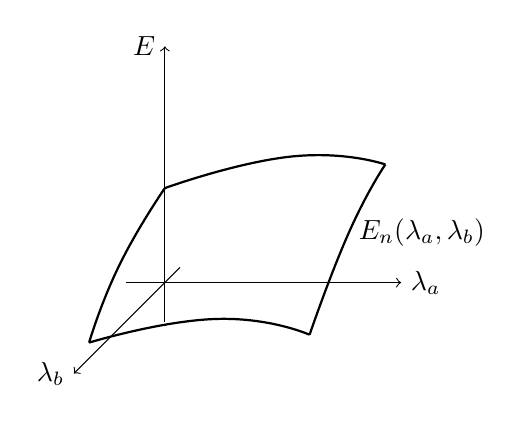
\begin{tikzpicture}
            \draw[->] (-0.5,0)--(3,0)node[right]{\(\lambda_a\)};
            \draw[->] (0,0,-0.5)--(0,0,3)node[left]{\(\lambda_b\)};
            \draw[->] (0,-0.5)--(0,3)node[left]{\(E\)};
            \draw[thick] plot[smooth, tension = 0.9] coordinates {(0,0.2,2.5) (0,0.8,1.5) (0,1.2,0)};
            \draw[thick] plot[smooth, tension = 0.9] coordinates {(0,0.2,2.5) (1.6,0.5,2.5) (2.8,0.3,2.5)};
            \draw[thick] plot[smooth, tension = 0.9] coordinates {(0,1.2,0) (1.6,1.6,0) (2.8,1.5,0)};
            \draw[thick] plot[smooth, tension = 0.9] coordinates {(2.8,0.3,2.5) (2.8,1.1,1.2) (2.8,1.5,0)};
            \node at (2.8,1.1,1.2)[right]{\(E_n(\lambda_a,\lambda_b)\)};
        \end{tikzpicture}
        \caption{The energy of state \(n\) as a function of the parameters \(\lambda_a\), \(\lambda_b\) when imposing two perturbations of comparable strengths.}
    \end{figure}

    We can then substitute these series ansatz into the Schr\"{o}dinger equation of the doubly perturbed Hamiltonian. Since \(\lambda_a\) and \(\lambda_b\) are independent variables, we need to gather and equate terms in each combination of them separately. The terms in \(\lambda_a\) and \(\lambda_b\) lead to two first-order equations
    \begin{align}
        (\hat{H}_a^{(1,0)}-E_n^{(1,0)})\ket{\psi_n^{(0,0)}}+(\hat{H}^{(0,0)}-E_n^{(0,0)})\psi_n^{(1,0)}&=0 \label{pertubration_a_equation}\\
        (\hat{H}_b^{(0,1)}-E_n^{(0,1)})\ket{\psi_n^{(0,0)}}+(\hat{H}^{(0,0)}-E_n^{(0,0)})\psi_n^{(0,1)}&=0\,, \label{pertubration_b_equation}
    \end{align}
    and contracting with \(\bra{\psi_n^{(0,0)}}\equiv\bra{n}\) yields two first-order energy expressions analogous to (\ref{first_order_energy})
    \begin{align}
        E_n^{(1,0)}&=\expval{\hat{H}_a^{(1,0)}}{n}\\
        E_n^{(0,1)}&=\expval{\hat{H}_b^{(0,1)}}{n}\,.
    \end{align}
    The second-equations in \(\lambda_a^2\) and \(\lambda_b^2\) are analogous to (\ref{perturbation_eqn_second}). However, we also have a second-order equation in \(\lambda_a\lambda_b\) containing cross terms
    \begin{equation}
        (\hat{H}^{(0,0)}-E_n^{(0,0)})\ket{\psi_n^{(1,1)}}+(\hat{H}_a^{(1,0)}-E_n^{(1,0)})\ket{\psi_n^{(0,1)}}+(\hat{H}_b^{(0,1)}-E_n^{(0,1)})\ket{\psi_n^{(1,0)}}-E_n^{(1,1)}\ket{n}=0\,.
    \end{equation}
    Contracting with \(\bra{n}\) gives
    \begin{equation}
        E_n^{(1,1)}=\mel{n}{\hat{H}_a^{(1,0)}}{\psi_n^{(0,1)}}+\mel{n}{\hat{H}_b^{(0,1)}}{\psi_n^{(1,0)}}\,.
    \end{equation}

    \subsubsection{Interchange Theorem}
    This expression contains both \(\ket{\psi_n^{(1,0)}}\) and \(\ket{\psi_n^{(0,1)}}\) --- we can do slightly better than that. If we take inner products of (\ref{pertubration_a_equation}) and (\ref{pertubration_b_equation}) with \(\ket{\psi_n^{(0,1)}}\) and \(\ket{\psi_n^{(1,0)}}\), respectively, and we get two mixed second-order equations. From these two equations, we can easily get
    \begin{equation}
        \mel{n}{\hat{H}_a^{(1,0)}}{\psi_n^{(0,1)}}=\mel{\psi_n^{(1,0)}}{\hat{H}_b^{(0,1)}}{n}\,.
    \end{equation}
    This allows us to rewrite the mixed second-order energy as
    \begin{equation}
        E_n^{(1,1)}=\mel{n}{\hat{H}_a^{(1,0)}}{\psi_n^{(0,1)}}+\mel{\psi_n^{(0,1)}}{\hat{H}_a^{(1,0)}}{n}\,.
    \end{equation}
    This is known as the \textit{interchange theorem}. Analogous results hold for mixed higher-order energy expressions as well, although they are much more complicated.

    \begin{ex}
        \textit{Molecular polarisability.}

        In previous example, we have examined the polarisability of a hydrogen atom. Due to its spherical symmetry, the first-order energy vanishes, and a single number is sufficient to assign its (isotropic) polarisability. However, a molecule may possess a permanent dipole moment and its polarisability may be anisotropic. We must therefore consider the orientations of the molecules and the electric field.

        Suppose a molecule consists of a collection of \(N\) point charges (including nuclei and electrons) \(e_i\) located at positions \(\{\vb{r}_i\}\). In the presence of a uniform electric field \(\vb{\mathcal{E}}\), there is an extra energy, which we see as a perturbation, given by
        \begin{equation}
            \hat{H}^{(1)}=-\sum_{i=1}^{N}e_i\vb{\mathcal{E}}\vdot\vb{r}_i=-\vb{\mathcal{E}}\vdot\hat{\vb{\mu}}\,,
        \end{equation}
        where we define the \textit{dipole moment operator} to be
        \begin{equation}
            \hat{\vb{\mu}}=\sum_i e_i\vb{r}_i\,.
        \end{equation}
        In component form,
        \begin{equation}
            \hat{H}^{(1)}=-\sum_\beta \mathcal{E}_\beta\hat{\mu}_\beta\,,
        \end{equation}
        where \(\beta\in\{x,y,z\}\). These are three independent perturbations of comparable magnitudes.

        By the Hellmann--Feynman theorem, we can write
        \begin{equation}\label{molecular_energy_expansion_in_electric_field}
            E_0=E_0^{(0)}-\sum_\beta\mu_\beta^0\mathcal{E}_\beta-\frac{1}{2}\sum_{\beta,\gamma}\alpha_{\beta\gamma}\mathcal{E}_\beta\mathcal{E}_\gamma-\dots
        \end{equation}
        for \(\beta,\gamma\in\{x,y,z\}\), where \(\vb{\mu}^0\) is the permanent dipole moment vector and \(\alpha\) is the polarisability tensor. The first-order energy is
        \begin{equation}
            E_0^{(1)}=\mel{0}{\hat{H}^{(1)}}{0}=-\sum_\beta\mathcal{E}_\beta\mel{0}{\hat{\mu}_\beta}{0}\,,
        \end{equation}
        and we indeed have \(\vb{\mu}^0=\mel{0}{\hat{\vb{\mu}}}{0}\). For the second-order energy, we apply the Rayleigh--Schr\"{o}dinger result
        \begin{align}
            E_0^{(2)}&=-\sum_{j\ne 0}\frac{\abs{\mel{j}{-\vb{\mathcal{E}}\vdot\hat{\vb{\mu}}}{0}}^2}{E_j^{(0)}-E_0^{(0)}}\notag\\
            &=-\sum_{\beta,\gamma}\mathcal{E}_\beta\mathcal{E}_\gamma\sum_{j\ne 0}\frac{\mel{j}{\hat{\mu}_\beta}{0}\mel{0}{\hat{\mu}_\gamma}{j}}{E_j^{(0)}-E_0^{(0)}}\,.
        \end{align}
        We can identify the latter sum as \(\frac{1}{2}\alpha_{\beta\gamma}\), but the polarisability is usually put into a symmetric form, although any antisymmetric part will cancel in the total second-order energy in (\ref{molecular_energy_expansion_in_electric_field}). Therefore, we will choose the components of the polarisability to be in the symmetrised form
        \begin{equation}\label{molecular_polarisability}
            \alpha_{\beta\gamma}=\sum_{j\ne 0}\frac{\mel{j}{\hat{\mu}_\beta}{0}\mel{0}{\hat{\mu}_\gamma}{j}+\mel{j}{\hat{\mu}_\gamma}{0}\mel{0}{\hat{\mu}_\beta}{j}}{E_j^{(0)}-E_0^{(0)}}\,.
        \end{equation}
    \end{ex}

    \newpage
    \section{Degenerate Perturbation Theory}
    Degeneracy presents issues in the above formulation of perturbation theory. First, it is obvious to see that if any state is degenerate to the unperturbed state, the denominator in the Rayleigh--Schr\"{o}dinger sum (\ref{RS_first_order_wavefunction}) will be zero. This suggests that an arbitrarily small perturbation will cause an extremely dramatic shift in the degenerate states of the system.

    This is not an unfamiliar effect. If we put a small ball in a bowl, then it will stay at the distinct, non-degenerate ground state at the bottom. If we tilt the bowl slightly, then the ball will also move slightly in the direction we tilt it to find the new minimum. However, if we put a ball on a flat table, where any point on it is degenerate, tilting the table however slightly will make the ball run away to infinity in the direction we tilt it. Perturbation lifts degeneracy.

    Suppose we impose a perturbation that lifts the degeneracy, thereby leading to unique perturbed states. If we gradually decrease the strength \(\lambda\) of the perturbation to zero, we expect that the system will return to a particular linear combination of the degenerate unperturbed state. This combination should resemble the perturbed states for small \(\lambda\). The key to degenerate perturbation theory is thus to identify those correct zeroth-order wavefunctions stable to perturbation.

    \subsection{Secular Equations for the Unperturbed Wavefunctions}
    Suppose there is an \(M\)-fold degenerate state \(n\) with energy \(E_n^{(0)}\). We denote the \(i^{\text{th}}\) component of the unperturbed state by \(\ket{\psi_{ni}^{(0)}}\), \(i\in\{1,\dots,M\}\), where these degenerate wavefunctions are mutually orthogonal \(\braket{\psi_{ni}^{(0)}}{\psi_{nj}^{(0)}}=\delta_{ij}\). Any linear combination of these functions has unperturbed energy \(E_n^{(0)}\). We write the zeroth-order wavefunctions that perturbed states return to in the limit \(\lambda\to 0\) as \(\ket{\Phi_{nj}^{(0)}}\). They are just linear combinations of the basis \(\left\{\ket{\psi_{ni}^{(0)}}\right\}\), so we may write
    \begin{equation}
        \ket{\Phi_{nj}^{(0)}}=\sum_{i=1}^{M}\ket{\psi_{ni}^{(0)}}c_{ij}\,.
    \end{equation}
    The perturbation expansions of the states are therefore
    \begin{equation}
        \ket{\psi_{nj}(\lambda)}=\ket{\Phi_{nj}^{(0)}}+\lambda\ket{\psi_{nj}^{(1)}}+\lambda^2\ket{\psi_{nj}^{(2)}}+\dots\,,
    \end{equation}
    giving the first-order equations
    \begin{equation}
        (\hat{H}^{(0)}-E_n^{(0)})\ket{\psi_{nj}^{(1)}}+(\hat{H}^{(1)}-E_{nj}^{(1)})\sum_{i=1}^{M}\ket{\psi_{ni}^{(0)}}c_{ij}=0\,.
    \end{equation}
    Contracting with some \(\bra{\psi_{nk}^{(0)}}\) gives
    \begin{equation}\label{degenerate_secular_equation}
        \sum_i\mel{\psi_{nk}^{(0)}}{\hat{H}^{(1)}-E_{nj}^{(1)}}{\psi_{ni}^{(0)}}c_{ij}=0\,.
    \end{equation}
    This is a set of \(M\times M\) simultaneous equations for \(j,k\in\{1,\dots,M\}\), which we may put into the matrix form as
    \begin{equation}
        (\mathsf{H}^{(1)}-\mathsf{I}E_{nj}^{(1)})\vb{c}_j=0
    \end{equation}
    for \(j\in\{1,\dots,M\}\), where \(H^{(1)}_{ki}=\mel{\psi_{nk}^{(0)}}{\hat{H}^{(1)}}{\psi_{ni}^{(0)}}\) is the matrix element of \(\mathsf{H}^{(1)}\) in the degenerate basis \(\left\{\ket{\psi_{ni}^{(0)}}\right\}\), and \(\vb{c}_j=(c_{1j},\dots,c_{Mj})\). The non-trivial solutions for \(c_{ij}\) are given by the secular equation
    \begin{equation}
        \abs{\mathsf{H}^{(1)}-\mathsf{I}E_{nj}^{(1)}}=0\,.
    \end{equation}
    Therefore, the appropriate zeroth-order wavefunctions are given by the eigenvectors of \(\mathsf{H}^{(1)}\), with the first-order energies given by the eigenvalues. We would also add the additional constraint
    \begin{equation}
        \braket{\Phi_{nj}^{(0)}}{\Phi_{nj}^{(0)}}=\sum_{i}\abs{c_{ij}}^2=1
    \end{equation}
    so that the zeroth-order wavefunctions are normalised.

    Since \(\left\{\ket{\Phi_{ni}^{(0)}}\right\}\) diagonalises the perturbation Hamiltonian \(\mathsf{H}^{(1)}\) in the basis spanned by themselves
    \begin{equation}
        \mel{\Phi_{nk}^{(0)}}{\hat{H}^{(1)}}{\Phi_{nj}^{(0)}}=\delta_{kj}E_{nj}^{(1)}\,,
    \end{equation}
    we claim that the second-order energy for any one member of the degenerate set therefore involves a sum that excludes all members of the degenerate set
    \begin{equation}
        E_{nj}^{(2)}=-\sum_{m\ne n}\frac{\abs{\mel{m}{\hat{H}^{(1)}}{\Phi_{nj}^{(0)}}}^2}{E_m^{(0)}-E_n^{(0)}}\,.
    \end{equation}
    Unfortunately, the expression of the first-order wavefunction is not simple, and it is explained in the appendix \cref{Chap:degenerate_PT_first_order_wavefunction} together with the proof of this second-order energy expression.

    \begin{ex}
        \textit{Linear Stark effect in the hydrogen atom.}

        We have examined the response of the 1s orbital energy of a hydrogen atom to a small and uniform electric field. The energy shift is proportional to the square of the electric field in the leading order, so it is known as the \textit{quadratic Stark effect}. We treated it using non-degenerate perturbation theory because the 1s state of hydrogen is non-degenerate.
        
        To analyse the shift of the degenerate 2p energy levels, we must instead use the degenerate perturbation theory. For the perturbation Hamiltonian \(\hat{H}^{(1)}=z\), the matrix elements are evaluated as
        \begin{equation}
            \mathsf{H}^{(1)}=\begin{pmatrix}
                0 & 0 & 0 & 3 \\
                0 & 0 & 0 & 0 \\
                0 & 0 & 0 & 0 \\
                3 & 0 & 0 & 0
            \end{pmatrix}\,,
        \end{equation}
        where the only non-zero matrix elements are \(\mel{2\mathrm{s}}{\hat{H}^{(1)}}{2\mathrm{p_z}}=\mel{2\mathrm{p_z}}{\hat{H}^{(1)}}{2\mathrm{s}}=3\). Therefore, the \(\mathrm{2p_x}\) and \(\mathrm{2p_y}\) orbitals are unaffected by the electric field to first order. The other two perturbed orbitals are \(\ket{\Phi_{\pm}^{(0)}}=(\ket{\mathrm{2s}}\pm\ket{\mathrm{2p_z}})/\sqrt{2}\), with first-order energies \(E_\pm^{(1)}=\pm 3\).

        The electric field therefore partially lifts the degeneracy of the hydrogen atom's \(n=2\) states with energies \(E_\pm=-\frac{1}{8}\pm 3\mathcal{E}\), leaving two orbitals unaffected to the first order. This is known as the \textit{linear Stark effect}. In a many-electron atom, the \(\mathrm{2s}\) and \(\mathrm{2p_z}\) orbitals are no longer degenerate, and so the Stark effect is again quadratic.
    \end{ex}

    \subsection{Nearly Degenerate Perturbation Theory}
    If we have the state of interest non-degenerate, but very close in energy to some other states, we cannot use non-degenerate perturbation theory because although the individual terms in the Rayleigh--Schr\"{o}dinger sum do not blow up, the perturbation series may fail to converge even for very small \(\lambda\) as the perturbation gets easily larger than the energy level separation. We need nearly degenerate perturbation theory.

    Since we have
    \begin{equation}
        (\hat{H}^{(0)}-E_n^{(0)})\ket{\psi_{ni}^{(0)}}=0\,,
    \end{equation}
    we may multiply this expression by \(c_{ij}\) and add to the secular equation (\ref{degenerate_secular_equation}) multiplied by \(\lambda\) to get
    \begin{equation}
        \sum_i\mel{\psi_{nk}^{(0)}}{\hat{H}^{(0)}+\lambda\hat{H}^{(1)}-E_n^{(0)}-\lambda E_{nj}^{(1)}}{\psi_{ni}^{(0)}}c_{ij}=0
    \end{equation}
    for degenerate states. Since \(\hat{H}=\hat{H}^{(0)}+\lambda\hat{H}^{(1)}\) is the total Hamiltonian, and \(E_{nj}=E_n^{(0)}+\lambda E_{nj}^{(1)}\) is the total energy corrected to the first order. For a set of exactly degenerate states, solving the secular equations\footnote{This is essentially the Schr\"{o}dinger equation
    \begin{equation}
        \mathsf{H}\vb{c}_j=E_{nj}\vb{c}_j
    \end{equation}
    in the confined basis set of the nearly degenerate orbitals using the full Hamiltonian, so we should be convinced that this equation is appropriate whether the states are degenerate or not.}
    \begin{equation}
        (\mathsf{H}-\mathsf{I}E_{nj})\vb{c}_j=\vb{0}
    \end{equation}
    using the total Hamiltonian is entirely equivalent to solving for the secular equation for just the perturbing Hamiltonian in the degenerate perturbation theory.

    The advantage of this form of secular equation is that it can also be applied when a set of states lie close in energy but are not rigorously degenerate. We can think of this as redefining the \(\hat{H}^{(0)}\) and \(\hat{H}^{(1)}\) in a way such that the small differences in the energy of the unperturbed states is absorbed into the perturbation, so that the unperturbed states are now somehow degenerate.

    \begin{ex}
        \textit{Fermi resonance in \(\mathrm{CO_2}\).}

        Under harmonic approximation (\ref{harmonic_approximation}), the molecular vibrational potential can be approximated as a sum of quadratic potential, which can be decoupled into a sum of independent Hamiltonians of harmonic potentials (\ref{separated_harmonic_oscillators}). We will show later that the transition intensity between the initial state \(\ket{\psi_i}\) and the final state \(\ket{\psi_f}\) is proportional to the squared modulus of the transition dipole moment\footnote{See time-dependent perturbation theory later.}
        \begin{equation}
            \vb{R}_{f\leftarrow i}=\mel{\psi_f}{\hat{\vb{\mu}}}{\psi_i}\,.
        \end{equation}
        One can write the dipole moment operator into a sum of the normal coordinates \(Q_k\), which can in turn be written as a sum of the ladder operators \(\hat{a}_k\) and \(\hat{a}_k^\dagger\).\footnote{One can first integrate out the common electronic wavefunction to work out \(\hat{\vb{\mu}}(\vb{Q})\) as a function of nuclear coordinates only, then expand it around the equilibrium nuclear geometry. See \textit{B8: Symmetry} for detail.} This will show that only transitions between states in which the quantum number of only a single mode changes by one can happen, i.e. \(\Delta n_k = \pm 1\).

        However, anharmonicity brings interesting complications. Since raising and lowering operators no longer holds for anharmonic states, overtones and combination lines are now allowed. Moreover, the fact that the Hamiltonian itself changes leading to the coupling of normal modes can bring interesting features to the IR and Raman spectra. The harmonic states \(\ket{n_1,n_2,\dots}\) which originally diagonalises the harmonic Hamiltonian \(\mel{n_1',n_2',\dots}{\hat{H}_{\text{harmonic}}}{n_1,n_2,\dots}=\sum_i\omega_i(n_i+\frac{1}{2})\delta_{n_1n_1'}\delta_{n_2n_2'}\dots\) no longer does so. This effect can be particularly strong if the two states with the same symmetry happen to be close in energy. We will investigate this effect using nearly degenerate perturbation theory.

        The classic example is \(\mathrm{CO_2}\). We will take the harmonic approximation as the reference Hamiltonian. In this case, the molecule has 4 normal modes: a symmetric stretch \((Q_1)\) of symmetry \(\Sigma_g^+\), a doubly-degenerate bend \((Q_{2x},Q_{2y})\) of symmetry \(\Pi_u\) and an antisymmetric stretch \((Q_3)\) of symmetry \(\Sigma_u^+\). We label a vibrational state by the three quantum numbers \(\ket{n_1,n_2,n_3}\), where \(n_2=n_{2x}+n_{2y}\). Denoting \(Q_2^2=Q_{2x}^2+Q_{2y}^2\), the unperturbed Hamiltonian and energy are
        \begin{equation}
            \hat{H}^{(0)}=-\frac{1}{2}\left(\pdv[2]{}{Q_1}+\pdv[2]{}{Q_{2x}}+\pdv[2]{}{Q_{2y}}+\pdv[2]{}{Q_3}\right)+\frac{1}{2}(\omega_1^2Q_1^2+\omega_2^2Q_{2}^2+\omega_3^2Q_3^2)\,,
        \end{equation}
        \begin{equation}
            E_{n_1,n_2,n_3}^{(0)}=\left(n_1+\frac{1}{2}\right)\omega_1+\left(n_2+\frac{1}{2}\right)\omega_2+\left(n_3+\frac{1}{2}\right)\omega_3\,.
        \end{equation}

        \begin{figure}
            \centering
            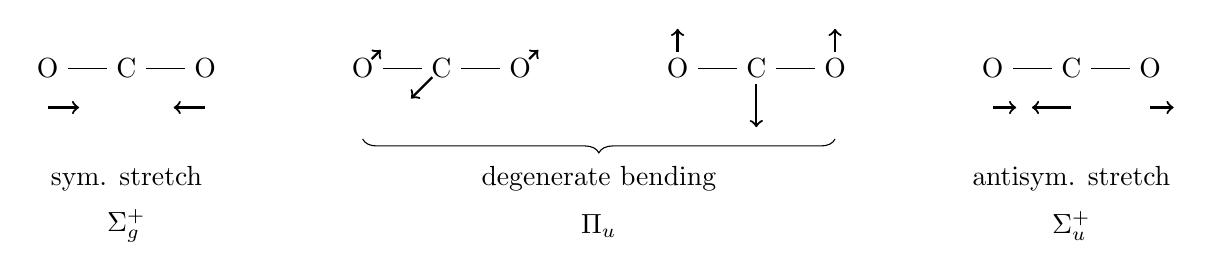
\begin{tikzpicture}
                \draw(0,0)node[fill=white]{O}--(1,0)node[fill=white]{C}--(2,0)node[fill=white]{O};
                \draw[->,thick] (0,-0.5)--(0.4,-0.5);
                \draw[->,thick] (2,-0.5)--(1.6,-0.5);
                \node at (1,-1.4){sym. stretch};
                \node at (1,-2){\(\Sigma_g^+\)};

                \begin{scope}[shift={(4,0)}]
                    \draw(0,0)node[fill=white]{O}--(1,0)node[fill=white]{C}--(2,0)node[fill=white]{O};
                    \draw[->,thick] (0,0,-0.3)--(0,0,-0.6);
                    \draw[->,thick] (1,0,0.3)--(1,0,1);
                    \draw[->,thick] (2,0,-0.3)--(2,0,-0.6);
                \end{scope}
                \begin{scope}[shift={(8,0)}]
                    \draw(0,0)node[fill=white]{O}--(1,0)node[fill=white]{C}--(2,0)node[fill=white]{O};
                    \draw[->,thick] (0,0.2)--(0,0.5);
                    \draw[->,thick] (1,-0.2)--(1,-0.75);
                    \draw[->,thick] (2,0.2)--(2,0.5);
                \end{scope}
                \draw [decorate,decoration={brace,amplitude=5pt,mirror}] (4,-0.9) -- (10,-0.9);
                \node at (7,-1.4){degenerate bending};
                \node at (7,-2){\(\Pi_u\)};
                \begin{scope}[shift={(12,0)}]
                    \draw(0,0)node[fill=white]{O}--(1,0)node[fill=white]{C}--(2,0)node[fill=white]{O};
                    \draw[->,thick] (0,-0.5)--(0.3,-0.5);
                    \draw[->,thick] (1,-0.5)--(0.5,-0.5);
                    \draw[->,thick] (2,-0.5)--(2.3,-0.5);
                    \node at (1,-1.4){antisym. stretch};
                    \node at (1,-2){\(\Sigma_u^+\)};
                \end{scope}
            \end{tikzpicture}
        \end{figure}
    \end{ex}

    The symmetric stretch and bend frequencies are \(\omega_1=1354.07\unit{cm}^{-1}\) and \(\omega_2=672.95\unit{cm}^{-1}\) respectively. Relative to the ground state, the doubly-excited bend \(\ket{020}\) at energy \(2\omega_2=1345.90\unit{cm}^{-1}\), lying just \(\Delta=8.17\unit{cm}^{-1}\) below the \(\ket{100}\) state. Moreover, the symmetry of the \(\ket{020}\) states are given by \(\Pi_u\otimes\Pi_u=\Sigma_g^+ + [\Sigma_g^-] +\Delta_g\), so the component of \(\ket{020}\) with zero angular momentum,
    \begin{equation}
        \ket{02^0 0}=\frac{1}{\sqrt{2}}(\ket{02_x 0}+\ket{02_y 0})
    \end{equation}
    has the correct symmetry to interact with \(\ket{100}\) if there exists appropriate coupling perturbation.

    We will add cubic potentials as a perturbation. Since the Hamiltonian must be totally symmetric, not all cubic potentials \(Q_iQ_jQ_k\) are permitted to be present. It turns out that the only allowed terms in the cubic potential are
    \begin{equation}
        \hat{H}^{(1)}=aQ_1^3+bQ_1Q_2^2+cQ_1Q_3^2\,.
    \end{equation}

    Using the nearly degenerate perturbation theory, we can see that this perturbing Hamiltonian indeed couples these two states. The total Hamiltonian matrix in the basis of the two states is given by
    \begin{equation}
        \mathsf{H}=\begin{pmatrix}
            \omega_1 & W \\
            W & 2\omega_2
        \end{pmatrix}\,,
    \end{equation}
    where \(W\) is the \textit{Fermi coupling constant} given by
    \begin{equation}
        W=\mel{100}{\hat{H}^{(0)}+\hat{H}^{(1)}}{02^0 0}=\mel{100}{bQ_1Q_2^2}{02^0 0}\,.
    \end{equation}
    This coupling is due to the cubic term \(Q_1Q_2^2\). We can again use ladder operators
    \begin{equation}
        Q_i=\frac{1}{\sqrt{2\omega_i}}(\hat{a}_i+\hat{a}_i^\dagger)
    \end{equation}
    to work this out. We write
    \begin{equation}
        \mel{100}{bQ_1Q_2^2}{02^0 0}=b\mel{1}{Q_1}{0}\mel{0}{Q_2^2}{2}\braket{0}{0}\,.
    \end{equation}
    The first term is easy to evaluate
    \begin{equation}
        \mel{1}{Q_1}{0}=\frac{1}{\sqrt{2\omega_1}}\mel{1}{\hat{a}+\hat{a}^\dagger}{0}=\frac{1}{\sqrt{2\omega_1}}\,,
    \end{equation}
    but the second degenerate mode is a bit more subtle. We need to expand it into its components
    \begin{align}
        \mel{0}{Q_2^2}{2^0}&=\frac{1}{\sqrt{2}}\left(\mel{0_x,0_y}{Q_{2x}^2}{2_x,0_y}+\mel{0_x,0_y}{Q_{2y}^2}{0_x,2_y}\right)\notag\\
        &=\sqrt{2}\mel{0}{Q_{2x}^2}{2_x}
    \end{align}
    as the two components are equivalent. Then
    \begin{align}
        \sqrt{2}\mel{0}{Q_{2x}^2}{2_x}&=\frac{1}{\sqrt{2}\omega_2}\mel{0}{\hat{a}^2}{2}\notag\\
        &=\frac{1}{\omega_2}\,.
    \end{align}
    Combining the results gives
    \begin{equation}
        W=\frac{b}{\sqrt{2\omega_1}\omega_2}\,.
    \end{equation}
    
    Solving the secular equation, we find that the perturbed states are separated by \(\sqrt{4W^2+\Delta^2}\), which is clearly bigger than the original separation \(\Delta\). This effect is known as the \textit{Fermi resonance}. The two lines are observed to be \(102.78\unit{cm}^{-1}\) apart in the Raman spectrum, implying \(\abs{W}=51.2\unit{cm}^{-1}\) --- a rather large coupling.

    The mixing of the vibrational states also means that the \(\ket{000}\to\ket{100}\) and \(\ket{000}\to\ket{02^0 0}\) transitions are no longer pure. Consequently, the latter transition, which would normally be a weak overtone, borrows intensity from the strong fundamental symmetric stretch. The pair of mixed levels are known as a \textit{Fermi dyad}.

    \begin{figure}[ht!]
        \centering
        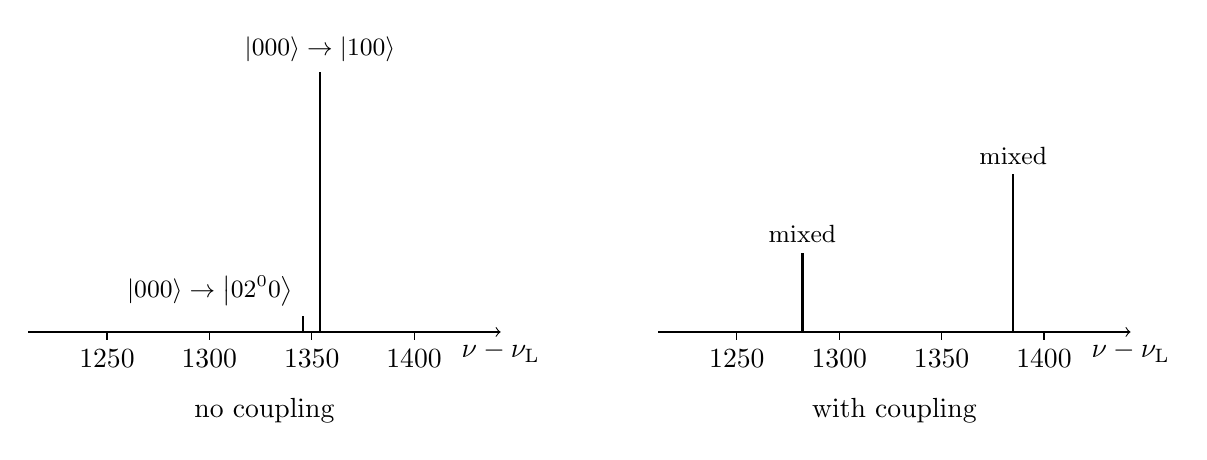
\begin{tikzpicture}
            \draw[->] (0,0)--(6,0)node[below]{\(\nu-\nu_{\text{L}}\)};
            \draw[thick] (3.4934,0)--(3.4934,0.2)node[above left]{\small \(\ket{000}\to\ket{02^0 0}\)};
            \draw[thick] (3.7058,0)--(3.7058,3.3)node[above]{\small \(\ket{000}\to\ket{100}\)};
            \draw (1,0)--(1,-0.1)node[below]{1250};
            \draw (2.3,0)--(2.3,-0.1)node[below]{1300};
            \draw (3.6,0)--(3.6,-0.1)node[below]{1350};
            \draw (4.9,0)--(4.9,-0.1)node[below]{1400};
            \node at (3,-1) {no coupling};

            \begin{scope}[shift={(8,0)}]
                \draw[->] (0,0)--(6,0)node[below]{\(\nu-\nu_{\text{L}}\)};
                \draw[thick] (4.51,0)--(4.51,2)node[above]{\small mixed};
                \draw[thick] (1.832,0)--(1.832,1)node[above]{\small mixed};
                \draw (1,0)--(1,-0.1)node[below]{1250};
                \draw (2.3,0)--(2.3,-0.1)node[below]{1300};
                \draw (3.6,0)--(3.6,-0.1)node[below]{1350};
                \draw (4.9,0)--(4.9,-0.1)node[below]{1400};
                \node at (3,-1) {with coupling};
            \end{scope}
        \end{tikzpicture}
    \end{figure}

    \begin{ex}
        \textit{Nearly free electron gas.}

        You should have met the concept of nearly free electron gas model for solids in Part IB Chemistry A. The idea of degenerate perturbation theory gives us some more insight on it.

        For our electron gas to be `nearly free', let's consider the situation where a particle moves in a region having a weakly periodic potential. By weakly periodic, we mean that the free energy of the particle is much greater than the periodic potential present: the particle floats well above a corrugated base. For example, let's assume that the underlying potential has the form
        \begin{equation}
            V(x)=2V\cos\left(\frac{2\pi x}{a}\right)=V(\ee^{\ii Gx}+\ee^{-\ii Gx})\,,
        \end{equation}
        where \(G=2\pi/a\) characterises the periodicity of the lattice in the form of a wavevector. Suppose the system has total length \(L=Na\), so it comprises \(N\) cells of size \(a\). For a real periodic potential in a periodic crystal lattice, we would replace this by a Fourier series, but let's now focus on this simple case.

        The fact that the periodic potential is weak makes it perfect for perturbation theory. We take the unperturbed Hamiltonian to be the free electron gas
        \begin{equation}
            \hat{H}^{(0)}=-\frac{\hbar^2}{2m}\pdv[2]{}{x}\,,
        \end{equation}
        and the unperturbed wavefunction is
        \begin{equation}
            \psi_k^{(0)}=\frac{1}{\sqrt{L}}\ee^{\ii kx}
        \end{equation}
        with unperturbed energy
        \begin{equation}
            E_k^{(0)}=\frac{\hbar^2k^2}{2m}\,.
        \end{equation}
        We impose the periodic boundary condition: \(\psi(x)=\psi(x+L)\) so \(k\) is discretised
        \begin{equation}
            k=\frac{2\pi n}{L}\,,\quad n\in\ZZ\,.
        \end{equation}
        The perturbing Hamiltonian is our periodic potential
        \begin{equation}
            \hat{H}^{(1)}=2V\cos\left(\frac{2\pi x}{a}\right)\,.
        \end{equation}

        To proceed, we would like to find the matrix elements of the perturbation
        \begin{align}
            \mel{k}{\hat{H}^{(1)}}{k'}&=\frac{2V}{L}\int_{0}^{L}\dd{x}\ee^{\ii(k'-k)x}\cos\left(\frac{2\pi x}{a}\right)\notag \\
            &=\frac{V}{L}\int_0^L\dd{x}\ee^{\ii(k'-k+G)x}+\ee^{\ii(k'-k-G)x}\notag\\
            &=V[\delta_{k-k',-G}+\delta_{k-k',+G}]\,.
        \end{align}
        Therefore, the only terms that survive are those for which
        \begin{equation}
            k'-k=\pm G=\pm\frac{2\pi}{a}\,,
        \end{equation}
        or
        \begin{equation}
            n'-n=\pm 1\,.
        \end{equation}
        State \(\ket{k}\) will only interact with states \(\ket{k+G}\) and \(\ket{k-G}\).

        In general, the states \(\ket{k}\) and \(\ket{k'}\) are non-degenerate, and the new energies can be calculated by non-degenerate perturbation theory
        \begin{align}
            E_k&=E_k^{(0)}+\expval{\hat{H}^{(1)}}{k}+\sum_{k'\ne k}\frac{\abs{\mel{k'}{\hat{H}^{(1)}}{k}}^2}{E_k^{(0)}-E_{k'}^{(0)}}\notag\\
            &=E_k^{(0)}+\frac{\abs{V}^2}{E_k^{(0)}-E_{k+G}^{(0)}}+\frac{\abs{V}^2}{E_k^{(0)}-E_{k-G}^{(0)}}\,.
        \end{align}
        However, the above method will break down in the neighbourhood of \(k\approx\pm\frac{\pi}{a}\), since by then, \(E_k^{(0)}\approx E_{k+G}^{(0)}\). We would then need to use nearly degenerate perturbation theory. For example, if we are interested in a state with \(k\approx +\frac{\pi}{a}\), which would interact with a nearly degenerate state at \(k'=k-\frac{2\pi}{a}\approx -\frac{\pi}{a}\), then the appropriate Hamiltonian matrix to diagonalise is
        \begin{equation}
            \mathsf{H}=\begin{pmatrix}
                E_k & V \\
                V & E_{k'}
            \end{pmatrix}\,,
        \end{equation}
        giving first-order energies
        \begin{equation}
            E=\frac{E_k+E_{k'}}{2}\pm\frac{1}{2}\sqrt{(E_k-E_{k'})^2+4V^2}\,.
        \end{equation}
        The two levels are now separated by a gap larger than their original separation:
        \begin{equation}
            \sqrt{(E_k-E_{k'})^2+4V^2}>(E_k-E_{k'})\,.
        \end{equation}
        If we consider \(k=+\frac{\pi}{a}\) and \(k'=-\frac{\pi}{a}\), so the two interacting states are exactly degenerate, then the perturbation will result in a gap of \(2V\). A band gap of \(2V\) is opened at \(k=\pm \frac{\pi}{a}\).

        \begin{figure}
            \centering
            % This file was created with tikzplotlib v0.10.1.
\begin{tikzpicture}

\definecolor{darkgray176}{RGB}{176,176,176}

\begin{axis}[
tick align=outside,
tick pos=left,
x grid style={darkgray176},
xlabel={\(\displaystyle k\,/\,\frac{\pi}{a}\)},
xmin=-1.98, xmax=1.98,
xtick style={color=black},
y grid style={darkgray176},
ylabel={\(\displaystyle E\)},
ymin=-0.292105809830368, ymax=3.4651744481256,
ytick style={color=black}
]
\addplot [semithick, black]
table {%
1.008 1.48353977253783
1.017 1.48419007933424
1.026 1.48565412836373
1.035 1.48792793934596
1.044 1.49100507431282
1.053 1.49487675954425
1.062 1.49953204749627
1.071 1.50495801194607
1.08 1.51113996859398
1.089 1.51806171290411
1.098 1.52570576701595
1.107 1.53405362805394
1.116 1.54308601100651
1.125 1.5527830804309
1.134 1.56312466645185
1.143 1.57409046176145
1.152 1.58566019750999
1.161 1.59781379704203
1.17 1.61053150734099
1.179 1.6237940087796
1.188 1.63758250433227
1.197 1.65187878979863
1.206 1.6666653068354
1.215 1.68192518071762
1.224 1.69764224477679
1.233 1.71380105341414
1.242 1.73038688548486
1.251 1.74738573971089
1.26 1.76478432362174
1.269 1.78257003735531
1.278 1.80073095348375
1.287 1.81925579386859
1.296 1.83813390439881
1.305 1.85735522832854
1.314 1.87691027880721
1.323 1.89679011108673
1.332 1.91698629479507
1.341 1.93749088658444
1.35 1.95829640339244
1.359 1.97939579649679
1.368 2.00078242649503
1.377 2.0224500393008
1.386 2.0443927432155
1.395 2.06660498710763
1.404 2.08908153971104
1.413 2.11181747003685
1.422 2.13480812888078
1.431 2.15804913139831
1.44 2.18153634071232
1.449 2.20526585251352
1.458 2.22923398061008
1.467 2.25343724338106
1.476 2.27787235108721
1.485 2.30253619399269
1.494 2.32742583125167
1.503 2.35253848051485
1.512 2.3778715082122
1.521 2.40342242047003
1.53 2.42918885462222
1.539 2.45516857127724
1.548 2.48135944690475
1.557 2.50775946690737
1.566 2.53436671914548
1.575 2.56117938788431
1.584 2.58819574813513
1.593 2.61541416036358
1.602 2.64283306554024
1.611 2.67045098051012
1.62 2.69826649365915
1.629 2.72627826085762
1.638 2.75448500166132
1.647 2.78288549575312
1.656 2.81147857960836
1.665 2.84026314336895
1.674 2.86923812791191
1.683 2.89840252209935
1.692 2.92775536019745
1.701 2.95729571945328
1.71 2.98702271781867
1.719 3.01693551181159
1.728 3.04703329450557
1.737 3.0773152936391
1.746 3.10778076983672
1.755 3.13842901493477
1.764 3.16925935040482
1.773 3.20027112586861
1.782 3.23146371769835
1.791 3.26283652769727
1.8 3.29438898185488
};
\addplot [semithick, black]
table {%
-0.999 0.485032127090968
-0.99 0.484109224290489
-0.981 0.482698596212544
-0.972 0.480806350053603
-0.963 0.478440945171834
-0.954 0.475613035623542
-0.945 0.472335278632546
-0.936 0.468622116663547
-0.927 0.464489541289122
-0.918 0.459954847045907
-0.909 0.455036383027919
-0.9 0.449753309155565
-0.891 0.444125362996907
-0.882 0.438172641815337
-0.873 0.431915403277947
-0.864 0.425373887066918
-0.855 0.418568158556071
-0.846 0.411517974787112
-0.837 0.404242672225654
-0.828 0.396761075198864
-0.819 0.389091423504915
-0.81 0.381251317421324
-0.801 0.37325767820172
-0.792 0.36512672211433
-0.783 0.356873946116782
-0.774 0.348514123358963
-0.765 0.34006130684026
-0.756 0.331528839703991
-0.747 0.32292937081836
-0.738 0.3142748744605
-0.729 0.305576673081858
-0.72 0.296845462284698
-0.711 0.288091337278383
-0.702 0.279323820208923
-0.693 0.270551887865669
-0.684 0.261783999365328
-0.675 0.253028123496433
-0.666 0.24429176547806
-0.657 0.235581992946137
-0.648 0.226905461030368
-0.639 0.218268436425825
-0.63 0.209676820396797
-0.621 0.201136170677594
-0.612 0.192651722256653
-0.603 0.184228407047366
-0.594 0.175870872462233
-0.585 0.167583498917024
-0.576 0.159370416299032
-0.567 0.151235519438774
-0.558 0.143182482628084
-0.549 0.135214773229705
-0.54 0.127335664424554
-0.531 0.11954824714306
-0.522 0.111855441226539
-0.513 0.104260005863579
-0.504 0.0967645493451161
-0.495 0.0893715381802636
-0.486 0.0820833056131715
-0.477 0.0749020595793163
-0.468 0.0678298901376335
-0.459 0.0608687764129395
-0.45 0.0540205930811149
-0.441 0.0472871164275793
-0.432 0.0406700300077171
-0.423 0.0341709299360828
-0.414 0.027791329829492
-0.405 0.0215326654274281
-0.396 0.0153962989116376
-0.387 0.00938352294528302
-0.378 0.00349556445063554
-0.369 -0.00226641185704316
-0.36 -0.00790130016300365
-0.351 -0.0134080504586383
-0.342 -0.0187856656450517
-0.333 -0.0240331988214016
-0.324 -0.0291497507457796
-0.315 -0.0341344674572735
-0.306 -0.0389865380486744
-0.297 -0.0437051925800454
-0.288 -0.0482897001240759
-0.279 -0.0527393669348001
-0.27 -0.0570535347318693
-0.261 -0.061231579093126
-0.252 -0.0652729079487652
-0.243 -0.0691769601708419
-0.234 -0.0729432042523498
-0.225 -0.0765711370705087
-0.216 -0.0800602827292952
-0.207 -0.0834101914766126
-0.198 -0.0866204386918348
-0.189 -0.089690623939779
-0.18 -0.0926203700874485
-0.171 -0.0954093224801686
-0.162 -0.0980571481739891
-0.153 -0.100563535221471
-0.144 -0.102928192008193
-0.135 -0.105150846637527
-0.126 -0.107231246361432
-0.117 -0.109169157055187
-0.108 -0.110964362734177
-0.0989999999999998 -0.112616665110986
-0.0899999999999999 -0.114125883191243
-0.0809999999999997 -0.11549185290676
-0.0719999999999998 -0.116714426784694
-0.0629999999999999 -0.117793473651575
-0.0539999999999998 -0.11872887837115
-0.0449999999999999 -0.119520541615158
-0.0359999999999998 -0.120168379666228
-0.0269999999999999 -0.120672324252229
-0.0179999999999998 -0.121032322411507
-0.0089999999999999 -0.121248336388536
2.22044604925031e-16 -0.121320343559643
0.00900000000000012 -0.121248336388536
0.0180000000000002 -0.121032322411507
0.0270000000000001 -0.120672324252229
0.0360000000000003 -0.120168379666228
0.0450000000000002 -0.119520541615158
0.0540000000000003 -0.11872887837115
0.0630000000000002 -0.117793473651575
0.0720000000000003 -0.116714426784694
0.0810000000000002 -0.115491852906759
0.0900000000000001 -0.114125883191243
0.0990000000000002 -0.112616665110986
0.108 -0.110964362734177
0.117 -0.109169157055187
0.126 -0.107231246361432
0.135 -0.105150846637527
0.144 -0.102928192008193
0.153 -0.100563535221471
0.162 -0.098057148173989
0.171 -0.0954093224801684
0.18 -0.0926203700874485
0.189 -0.0896906239397789
0.198 -0.0866204386918347
0.207 -0.0834101914766125
0.216 -0.0800602827292952
0.225 -0.0765711370705085
0.234 -0.0729432042523496
0.243 -0.0691769601708418
0.252 -0.0652729079487651
0.261 -0.0612315790931258
0.27 -0.057053534731869
0.279 -0.0527393669348
0.288 -0.0482897001240757
0.297 -0.0437051925800452
0.306 -0.0389865380486742
0.315 -0.0341344674572733
0.324 -0.0291497507457795
0.333 -0.0240331988214013
0.342 -0.0187856656450514
0.351 -0.0134080504586381
0.36 -0.00790130016300351
0.369 -0.00226641185704304
0.378 0.00349556445063582
0.387 0.00938352294528331
0.396 0.0153962989116377
0.405 0.0215326654274283
0.414 0.0277913298294923
0.423 0.0341709299360831
0.432 0.0406700300077172
0.441 0.0472871164275795
0.45 0.0540205930811152
0.459 0.0608687764129399
0.468 0.0678298901376337
0.477 0.0749020595793165
0.486 0.0820833056131719
0.495 0.089371538180264
0.504 0.0967645493451165
0.513 0.104260005863579
0.522 0.111855441226539
0.531 0.11954824714306
0.54 0.127335664424554
0.549 0.135214773229706
0.558 0.143182482628084
0.567 0.151235519438774
0.576 0.159370416299033
0.585 0.167583498917024
0.594 0.175870872462233
0.603 0.184228407047367
0.612 0.192651722256654
0.621 0.201136170677594
0.63 0.209676820396798
0.639 0.218268436425826
0.648 0.226905461030368
0.657 0.235581992946137
0.666 0.24429176547806
0.675 0.253028123496433
0.684 0.261783999365329
0.693 0.27055188786567
0.702 0.279323820208923
0.711 0.288091337278383
0.72 0.296845462284699
0.729 0.305576673081859
0.738 0.3142748744605
0.747 0.32292937081836
0.756 0.331528839703991
0.765 0.34006130684026
0.774 0.348514123358964
0.783 0.356873946116782
0.792 0.365126722114331
0.801 0.373257678201721
0.81 0.381251317421325
0.819 0.389091423504915
0.828 0.396761075198864
0.837 0.404242672225655
0.846 0.411517974787112
0.855 0.418568158556071
0.864 0.425373887066918
0.873 0.431915403277947
0.882 0.438172641815338
0.891 0.444125362996907
0.9 0.449753309155566
0.909 0.455036383027919
0.918 0.459954847045907
0.927 0.464489541289122
0.936 0.468622116663547
0.945 0.472335278632546
0.954 0.475613035623542
0.963 0.478440945171834
0.972 0.480806350053603
0.981 0.482698596212544
0.99 0.484109224290489
0.999 0.485032127090968
};
\addplot [semithick, black]
table {%
-1.8 3.29438898185488
-1.791 3.26283652769727
-1.782 3.23146371769835
-1.773 3.2002711258686
-1.764 3.16925935040482
-1.755 3.13842901493477
-1.746 3.10778076983672
-1.737 3.0773152936391
-1.728 3.04703329450557
-1.719 3.01693551181159
-1.71 2.98702271781867
-1.701 2.95729571945327
-1.692 2.92775536019745
-1.683 2.89840252209935
-1.674 2.8692381279119
-1.665 2.84026314336895
-1.656 2.81147857960836
-1.647 2.78288549575311
-1.638 2.75448500166131
-1.629 2.72627826085761
-1.62 2.69826649365915
-1.611 2.67045098051012
-1.602 2.64283306554024
-1.593 2.61541416036357
-1.584 2.58819574813513
-1.575 2.56117938788431
-1.566 2.53436671914548
-1.557 2.50775946690737
-1.548 2.48135944690474
-1.539 2.45516857127724
-1.53 2.42918885462222
-1.521 2.40342242047003
-1.512 2.3778715082122
-1.503 2.35253848051485
-1.494 2.32742583125167
-1.485 2.30253619399268
-1.476 2.27787235108721
-1.467 2.25343724338106
-1.458 2.22923398061009
-1.449 2.20526585251352
-1.44 2.18153634071231
-1.431 2.15804913139831
-1.422 2.13480812888078
-1.413 2.11181747003685
-1.404 2.08908153971104
-1.395 2.06660498710763
-1.386 2.0443927432155
-1.377 2.02245003930079
-1.368 2.00078242649503
-1.359 1.97939579649679
-1.35 1.95829640339244
-1.341 1.93749088658443
-1.332 1.91698629479507
-1.323 1.89679011108673
-1.314 1.87691027880721
-1.305 1.85735522832854
-1.296 1.83813390439881
-1.287 1.81925579386859
-1.278 1.80073095348375
-1.269 1.78257003735531
-1.26 1.76478432362174
-1.251 1.74738573971089
-1.242 1.73038688548486
-1.233 1.71380105341414
-1.224 1.69764224477678
-1.215 1.68192518071762
-1.206 1.6666653068354
-1.197 1.65187878979863
-1.188 1.63758250433227
-1.179 1.6237940087796
-1.17 1.61053150734099
-1.161 1.59781379704203
-1.152 1.58566019750999
-1.143 1.57409046176145
-1.134 1.56312466645185
-1.125 1.5527830804309
-1.116 1.54308601100651
-1.107 1.53405362805394
-1.098 1.52570576701595
-1.089 1.5180617129041
-1.08 1.51113996859398
-1.071 1.50495801194607
-1.062 1.49953204749627
-1.053 1.49487675954425
-1.044 1.49100507431282
-1.035 1.48792793934596
-1.026 1.48565412836373
-1.017 1.48419007933425
-1.008 1.48353977253783
};
\end{axis}

\end{tikzpicture}

            \caption{The dispersion curve of a nearly free electron gas model calculated using nearly degenerate perturbation theory, with \(V\) set to be \(0.5\) in arbitrary units. A band gap of \(1\) is opened at \(k=\pm\frac{\pi}{a}\).}
        \end{figure}

        For a real periodic potential that can be written in a Fourier series
        \begin{equation}
            V(x)=\sum_{m=1}^{\infty}V_m\cos\left(\frac{m\pi x}{a}\right)\,,
        \end{equation}
        the term \(\cos(m\pi x/a)=\ee^{+\ii mGx}+\ee^{-\ii mGx}\) will lead to the interaction between \(\ket{k}\) and \(\ket{k\pm m G}\), and hence band gaps will open at \(\pm\frac{m\pi}{a}\). For a most general periodic potential, \(V_m\ne 0\) for all \(m\), so band gaps are opened at all positive integer multiples of \(\pm\frac{\pi}{a}\), leading to the band structure you met in IB Chemistry A.
    \end{ex}

    \newpage

    \section{Time-Dependent Systems}\label{Chap:TDPT}
    \subsection{Time-Dependent Schr\"{o}dinger Equation}
    For a time-dependent system, we have to turn to consider the time-dependent Schr\"{o}dinger equation
    \begin{equation}
        \hat{H}\Psi(\vb{x},t)=\ii\hbar\pdv{\Psi(\vb{x},t)}{t}\,.
    \end{equation}
    The wavefunction is now a function of time as well as the spatial coordinates. We will first focus on the special case that the Hamiltonian is independent of time. This is then a straightforward first-order differential equation in time, with solutions given by
    \begin{equation}
        \Psi(\vb{x},t)=\ee^{-\ii\hat{H}t/\hbar}\Psi(\vb{x},0)\,,
    \end{equation}
    where \(\hat{U}(t,0)=\ee^{-\ii\hat{H}t/\hbar}\) is the \textit{time evolution operator} and \(\Psi(\vb{x},0)\), the wavefunction at time \(t=0\), solves the time-independent Schr\"{o}dinger equation
    \begin{equation}
        \hat{H}\Psi(\vb{x},0)=E_k\Psi(\vb{x},0)\,,
    \end{equation}
    where it is common to denote the time-independent wavefunction as \(\psi_k(\vb{x})\equiv \Psi(\vb{x},0)\). \(\ee^{-\ii\hat{H}t/\hbar}\) is the \textit{time-evolution operator}, which is unitary. The exponential of the operator is defined via the Maclaurin series
    \begin{align}
        \ee^{-\ii\hat{H}t/\hbar}\ket{\psi_k}&=1-\ii\frac{t}{\hbar}\hat{H}\ket{\psi_k}-\frac{t^2}{2\hbar^2}\hat{H}^2\ket{\psi_k}+\ii\frac{t^3}{6\hbar^3}\hat{H}^3\ket{\psi_k}+\dots\notag \\
        &=1-\ii\frac{t}{\hbar}E_k\ket{\psi_k}-\frac{t^2}{2\hbar^2}E_k^2\ket{\psi_k}+\ii\frac{t^3}{6\hbar^3}E_k^3\ket{\psi_k}\notag \\
        &=\ee^{-\ii E_k t/\hbar}\ket{\psi_k}\,.
    \end{align}
    Therefore, for a time-independent Hamiltonian, there is a special class of solutions that can be written as
    \begin{equation}
        \Psi(\vb{x},t)=\ee^{-\ii E_k t/\hbar}\psi_k(\vb{x})\,.
    \end{equation}
    These are known as \textit{stationary states} because it is just a time-independent state multiplied by a phase factor rotating with time. None of the physical observables will change with time, as one might expect by the action of a unitary operator.

    From now on, we will adopt atomic units, so all \(\hbar\)'s are gone from our expressions.
    
    \subsection{Ehrenfest Theorem}
    The Ehrenfest theorem concerns the time evolution of expectation values of physical observables. We begin with
    \begin{align}
        \dv{}{t}\eval{A}&=\dv{}{t}\expval{\hat{A}}{\Psi}\notag\\
        &=\mel{\pdv{\Psi}{t}}{\hat{A}}{\Psi}+\expval{\pdv{\hat{A}}{t}}{\Psi}+\mel{\Psi}{\hat{A}}{\pdv{\Psi}{t}}\,.
    \end{align}
    We can use the time-dependent Schr\"{o}dinger equation to substitute for the time derivatives of the wavefunction
    \begin{align}
        \dv{}{t}\eval{A}&=\mel{-\ii\hat{H}\Psi}{\hat{A}}{\Psi}+\expval{\pdv{\hat{A}}{t}}{\Psi}+\mel{\Psi}{\hat{A}}{-\ii\hat{H}\Psi}\notag \\
        &=\ii\expval{\hat{H}\hat{A}}{\Psi}+\eval{\pdv{\hat{A}}{t}}-\ii\expval{\hat{A}\hat{H}}{\Psi}\notag \\
        &=-\ii\eval{[\hat{A},\hat{H}]}+\eval{\pdv{\hat{A}}{t}}\,.
    \end{align}
    This result is general, but the Ehrenfest theorem relates to the specific case of position and momentum.
    \begin{thm}[Ehrenfest theorem]
        \begin{align}
            m\dv{}{t}\eval{x}&=\eval{p}\\
            \dv{}{t}\eval{p}&=-\eval{\dv{V(x)}{x}}\,.
        \end{align}
    \end{thm}
    They are the quantum equivalents of the familiar classical expressions
    \begin{align}
        p&=mv \\
        F&=ma\,,
    \end{align}
    but they are not quite the same. To match up with the classical expression exactly, we would need
    \begin{equation}
        \dv{}{t}\eval{p}\stackrel{?}{=}-\dv{V(\eval{x})}{x}\,,
    \end{equation}
    but this would imply
    \begin{equation}
        \eval{\dv{V(x)}{x}}\stackrel{?}{=}\dv{V(\eval{x})}{x}\,,
    \end{equation}
    which is not in general true. For example, if we set \(V(x)=x^3\), then this equation implies \(\eval{x^2}\stackrel{?}{=}\eval{x}^2\). The difference in them is related to \(\Delta x\), so if we are approaching the classical limit, \(\Delta x\to 0\), then the Ehrenfest equations would approach Newton's equations. This is an example of the correspondence principle.

    It is possible to go the other way around and derive the time-dependent Schr\"{o}dinger equation from the Ehrenfest theorem, so the Ehrenfest theorem is just as fundamental as the Schr\"{o}dinger equation and could be used as the starting point for quantum mechanics.

    \subsection{Time-Dependent Perturbation Theory}
    We will consider the time-dependent Hamiltonian of the general form
    \begin{equation}
        \hat{H}(\vb{x},t)=\hat{H}^{(0)}(\vb{x})+\lambda\hat{H}^{(1)}(\vb{x},t)\,,
    \end{equation}
    where the unperturbed Hamiltonian is time-independent and we know its eigenstates \(\psi_k(\vb{x})\) and eigenvalues \(E_k\) exactly. The time dependence appears only in the perturbation \(\hat{H}^{(1)}\), which is `small'. In the absence of the perturbation, there are stationary solutions
    \begin{equation}
        \ket{\Psi_k(t)}=\ee^{-\ii E_k t}\ket{\psi_k}\,,
    \end{equation}
    where
    \begin{equation}
        \hat{H}^{(0)}\ket{\psi_k}=E_k\ket{\psi_k}\,.
    \end{equation}
    We have dropped the superscript \((0)\) on \(\psi_k\) and \(E_k\) because the stationary state is necessarily unperturbed.

    As in the Rayleigh--Schr\"{o}dinger perturbation theory, we now expand the perturbed wavefunction in terms of the unperturbed state. In the method developed by Dirac, known as the variation of constants,\footnote{This is formally known as the \textit{interaction picture}, or the \textit{Dirac picture}. We will not introduce it in the main text, because we can work out the first-order time-dependent perturbation theory without using this formal framework. However, this is very useful if we want to go to higher orders to explain things like Raman scattering, so it is introduced in the appendix, together with the other two pictures: the Schr\"{o}dinger picture and the Heisenberg picture.} the coefficients depend on time
    \begin{equation}
        \ket{\Psi(t)}=\sum_k a_k(t)\ket{\Psi_k(t)}=\sum_k a_k(t) \ee^{-\ii E_k t} \ket{\psi_k}\,.
    \end{equation}
    We must be able to do this because \(\{\ket{\psi_k}\}\) is a complete orthonormal basis, so we can expand \(\ket{\Psi(t)}\) at each time.

    There is no subscript to label the state, since the state is changing in time. Moreover, the squared modulus of the coefficient is the probability of observing the system in the stationary state \(k\) with energy \(E_k\) at time \(t\).\footnote{Technically the stationary state \(\Psi_k\) is the energy eigenstate of the system only if perturbing Hamiltonian is not present, so we should remove it before measuring the energy if we are interested in the question `which state of \(\Psi_k\) has our system evolved into'.} Substituting into the time-dependent Schr\"{o}dinger equation, we get
    \begin{align}
        \sum_k a_k\left(E_k+\lambda\hat{H}^{(1)}\right)\ket{\Psi_k}&=\ii\sum_k\left(\dv{a_k}{t}-\ii a_kE_k\right)\ket{\Psi_k}\notag\\
        \lambda\sum_k\hat{H}^{(1)}a_k\ket{\Psi_k}&=\ii\sum_k\dv{a_k}{t}\ket{\Psi_k}\,.
    \end{align}
    To work out the contribution of a particular \(\ket{\Psi_j}\), we contract it with \(\bra{\Psi_j}=\ee^{+\ii E_j t}\bra{\psi_j}\) and get
    \begin{equation}
        \lambda\sum_k a_k \ee^{-\ii(E_k-E_j)t}\mel{j}{\hat{H}^{(1)}}{k}=\ii\sum_k\dv{a_k}{t}\ee^{-\ii(E_k-E_j)t}\braket{j}{k}\,,
    \end{equation}
    and by orthogonality of unperturbed wavefunctions, we get
    \begin{equation}\label{coupled_equation_of_coeff}
        \dv{a_j}{t}=-\ii\lambda\sum_k \hat{H}_{jk}^{(1)}(t)a_k(t) \ee^{\ii\omega_{jk}t}\,,
    \end{equation}
    where \(\omega_{jk}=E_j-E_k\). This is a coupled system of differential equations, telling us how the weights of various states evolve with time. The rate of change of one weight depends on the current values of all the weights.

    To break the interdependency of the coefficients, we must make approximations. We expand the coefficients \(a_k(t)\) in a power series of \(\lambda\)
    \begin{equation}
        a_k(t)=a_k^{(0)}(0)+\lambda a_k^{(1)}(t)+\lambda^2a_k^{(2)}(t)+\dots
    \end{equation}
    Note that the unperturbed system is time-independent, so \(a_k^{(0)}\) does not depend on time. We can then solve for each power in \(\lambda\) individually. Note the presence of \(\lambda\) on the right-hand side of (\ref{coupled_equation_of_coeff}) means that the dependence of first-order terms are given purely by the time-independent zeroth-order terms. Therefore we have successfully decoupled the time dependence of the coefficients. We have
    \begin{align}
        \dv{a_j^{(0)}}{t}&= 0\\
        \dv{a_j^{(1)}}{t}&=-\ii\sum_k a_k^{(0)}(0)\hat{H}_{jk}^{(1)}(t)\ee^{\ii\omega_{jk}t}\\
        &\quad\vdots\notag
    \end{align}
    The zeroth-order equation reassures that the \(a_j\) is unchanging because \(\hat{H}^{(0)}\) is time-independent. The first-order equation is our main interest, telling us how the state is evolving to the leading order.

    If we now suppose that at time \(t=0\), the system is known to be in one of the stationary states \(\ket{\psi_n}\), such that \(a_k^{(0)}=\delta_{nk}\), we can remove the sum and get
    \begin{equation}
        \dv{a_j}{t}=-\ii H_{jn}^{(1)}(t)\ee^{\ii\omega_{jn}t}\,,
    \end{equation}
    where we dropped the superscript because we are only interested in the first-order contribution, so this is the rate of change of our total \(a_k\). We may integrate with respect to time and get
    \begin{equation}\label{first_order_time_dependent_perturbation}
        a_j(t)=-\ii\int_{0}^{t}\dd{t'}H_{jn}^{(1)}(t')\ee^{\ii\omega_{jn}t'}\,.
    \end{equation}
    Heuristically, this amounts to considering only direct transitions from initial state \(\ket{n}\) to the state \(\ket{j}\) of interest. Excitations that proceed via intermediate states are neglected. We therefore derived a first-order result, where the perturbation is only allowed to act once. A second-order expression can be obtained by substituting (\ref{first_order_time_dependent_perturbation}) back to (\ref{coupled_equation_of_coeff}), but we will do it using the interaction picture in the appendix \cref{Chap:Three_Pictures}.

    \begin{ex}
        \textit{A slowly-switched-on perturbation.}

        Let's first investigate the response of a system to a perturbation that is gradually switched on and approaching a constant value. A possible form of this can be
        \begin{equation}
            \hat{H}^{(1)}(\vb{x},t)=(1-\ee^{-kt})\hat{V}(\vb{x})
        \end{equation}
        for some time-independent perturbation \(\hat{V}(\vb{x})\). Suppose we are initially in a state \(\ket{n}\), then the coefficient of state \(\ket{j}\) is
        \begin{align}
            a_j(t)&=-\ii V_{jn}\int_{0}^{t}\dd{t'}(1-\ee^{-kt'})\ee^{\ii\omega_{jn}t'}\notag\\
            &=-\ii V_{jn}\left(\frac{\ee^{\ii\omega_{jn}t}-1}{\ii\omega_{jn}}-\frac{\ee^{(\ii\omega_{jn}-k)t}-1}{\ii\omega_{jn}-k}\right)\,,
        \end{align}
        where \(V_{jn}=\mel{j}{\hat{V}}{n}\). After some non-trivial amount of algebra, one may show that the probability of transition from state \(\ket{n}\) to \(\ket{j}\), \(\abs{a_j(t)}^2\), is given by
        \begin{equation}\label{two_level_transition_probability}
            \abs{a_j(t)}^2=\frac{V_{jn}^2}{\omega_{jn}^2}\frac{[\omega_{jn}(1-\ee^{-kt})-k\sin\omega_{jn}t]^2+k^2(1-\cos\omega_{jn}t)^2}{k^2+\omega_{jn}^2}\,.
        \end{equation}
        This is not a tidy expression, and we will have a brief analysis of this later. We will now focus on the long-time behaviour limit, \(kt\gg 1\), and suppose that the switching is very slow in comparison with the relevant frequency offset, \(k\ll\omega_{jn}\). We then have
        \begin{equation}
            a_j(t)=-\ii V_{jn}\frac{\ee^{\ii\omega_{jn}t}}{\ii\omega_{jn}}=-\frac{V_{jn}}{E_j-E_n}\ee^{\ii\omega_{jn}t}\,.
        \end{equation}
        Evidently, this result cannot be applied to the initial state \(\ket{n}\), but we argue that since the perturbation is small, the transition is negligible and we will have \(a_n(t)=a_n(0)=1\) to the leading order. The complete wavefunction is
        \begin{align}
            \Psi(t)&=\Psi_n(t)+\sum_{j\ne n}a_j(t)\Psi_j(t)\notag\\
            &=\ket{n} \ee^{-\ii E_n t}-\sum_{j\ne n}\frac{V_{jn}}{E_j-E_n}\ee^{\ii\omega_{jn}t}\ket{j}\ee^{-\ii E_j t}\notag\\
            &=\left(\ket{n}-\sum_{j\ne n}\frac{V_{jn}}{E_j-E_n}\ket{j}\right)\ee^{-\ii E_n t}\,.
        \end{align}
        We observe that this is exactly the Rayleigh--Schr\"{o}dinger sum of the first-order wavefunction multiplied by a time-dependent phase factor of constant modulus. Therefore, in the long-time limit,
        \begin{equation}
            \Psi(t)=(\psi_n^{(0)}+\psi_n^{(1)})\ee^{-\ii E_n t}\,,
        \end{equation}
        which is just the first-order time-independent perturbation result multiplied with its phase factor.

        This justifies the application of time-independent perturbation theory to the study of external perturbations to a system, provided that the perturbation is switched on sufficiently slowly. The system remains in the state that can be properly labelled as \(n\) described by the time-independent perturbation theory. We say that such a system is \textit{adiabatic}, standing for slowly varying. This is the \textit{adiabatic theorem} due to Max Born and Vladimir Fock.
        \begin{thm}[Adiabatic theorem]
            A physical system remains in its instantaneous eigenstate if a given perturbation is acting on it slowly enough and if there is a gap between the eigenvalue and the rest of the Hamiltonian's spectrum.
        \end{thm}
        This is closely linked to the adiabatic (Born--Oppenheimer) approximation, in which since the motion of the nuclei is varying slowly with respect to electrons, the electrons can be thought of as in the electronic eigenstates of the instantaneous nuclear geometry at each instant.

        If \(k\) is not sufficiently small compared to \(\omega\) then the switching cannot be regarded as adiabatically slow, and we must use the more complex form of the transition probability (\ref{two_level_transition_probability}). We consider a two-level system with \(E_0=0\) and \(E_1=\omega\), initially residing in the ground state, and a perturbation \(V_{01}=V\) is turned on with rate \(k\). The transition probability is plotted in scaled time \(\omega t\) and is normalised by the adiabatic long-time limit \(V^2/\omega^2\).

        \begin{figure}
            \centering
            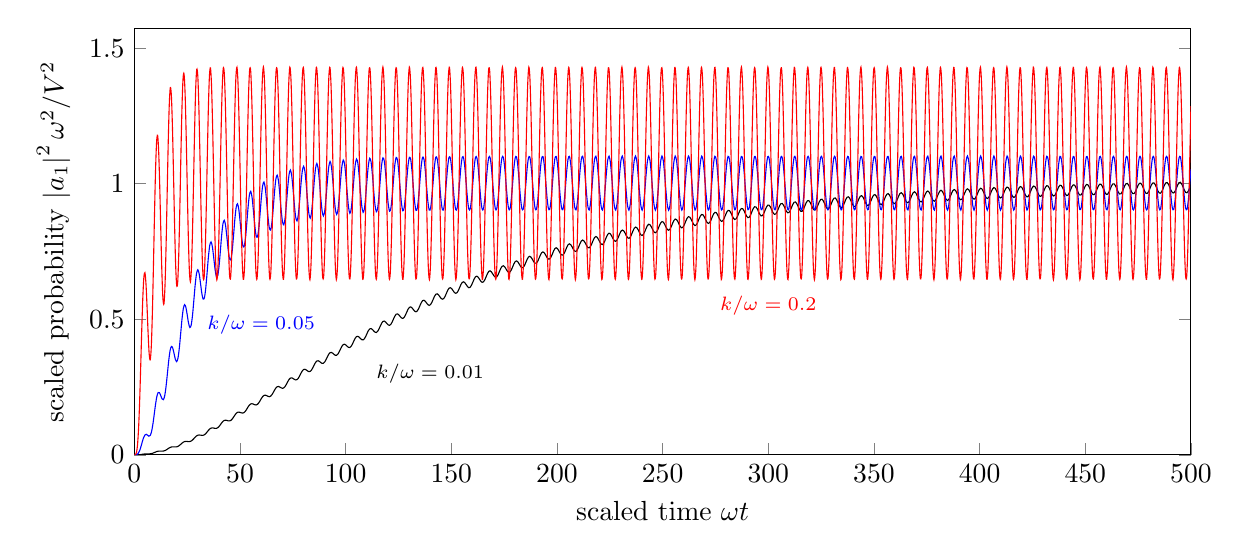
\begin{tikzpicture}
                \begin{axis}[width=15cm,height=7cm,xmin=0,xmax=500,ymin=0,xtick pos=lower,xlabel={scaled time \(\omega t\)},ylabel={scaled probability \(\abs{a_1}^2\omega^2/V^2\)}]
                    \addplot[domain=0:500,samples=800,smooth]{(0.02*(1-cos(deg(x)))-2*(1-exp(-0.01*x))*sin(deg(x))+100*(1-exp(-0.01*x))^2)/100.01};
                    \addplot[domain=0:500,samples=800,smooth,blue]{(0.02*(1-cos(deg(x)))-0.4*(1-exp(-0.05*x))*sin(deg(x))+4*(1-exp(-0.05*x))^2)/4.01};
                    \addplot[domain=0:500,samples=1000,smooth,red]{(0.02*(1-cos(deg(x)))-0.1*(1-exp(-0.2*x))*sin(deg(x))+0.25*(1-exp(-0.2*x))^2)/0.26};
                    \node at (140,0.3){\scriptsize\(k/\omega=0.01\)};
                    \node[blue] at (60,0.48){\scriptsize\(k/\omega=0.05\)};
                    \node[red] at (300,0.55){\scriptsize\(k/\omega=0.2\)};
                \end{axis}
            \end{tikzpicture}
            \caption{Scaled probability of transition to excited state in a two-level system when a perturbation is switched on at different rates.}
        \end{figure}

        We see that switching at a finite rate induces oscillations in the occupation of the upper state, and the magnitude of the oscillation increases with the switching rate. The oscillations continue even after their mean has settled down to its final value. If you are careful enough, you can see that the mean does not coincide with the adiabatic limit.\footnote{You may replace all the oscillatory terms (\(\sin\) and \(\cos\)) with 0 in (\ref{two_level_transition_probability}), and get
        \begin{equation}
            \frac{k^2+\omega^2(1-\ee^{-kt})^2}{k^2+\omega^2}\,,
        \end{equation}
        which does tend to \(1\) as \(t\to\infty\) regardless of \(k\). However, oscillatory terms do shift the mean value because it is squared.}
    \end{ex}

    \begin{ex}
        \textit{Fermi's golden rule.}

        We now study the interaction of oscillating electromagnetic radiation with atoms or molecules. We will investigate the stimulated absorption and stimulated emission, which should be familiar from \textit{A3: High Resolution Molecular Spectroscopy}.

        The most general form of the perturbing Hamiltonian should be
        \begin{equation}
            \hat{H}^{(1)}(t)=\hat{V} \ee^{\ii\omega t}+\hat{V}^\dagger \ee^{-\ii\omega t}
        \end{equation}
        for some time-independent operator \(\hat{V}\). We let \(\hat{V}\) be Hermitian so that
        \begin{equation}\label{EM_Wave_Hamiltonian}
            \hat{H}^{(1)}=2\hat{V}\cos\omega t\,.
        \end{equation}
        We insert this into (\ref{first_order_time_dependent_perturbation}) and we will get
        \begin{equation}
            a_j(t)=-V_{jn}\left(\frac{\ee^{\ii(\omega_{jn}+\omega)t}-1}{\omega_{jn}+\omega}+\frac{\ee^{\ii(\omega_{jn}-\omega)t}-1}{\omega_{jn}-\omega}\right)\,.
        \end{equation}
        We can see that if \(\omega_{jn}\) is positive (\(\ket{j}\) above \(\ket{n}\)) and \(\omega\) is close to \(\omega_{jn}\), then the second fraction will dominate. This corresponds to a \textit{stimulated absorption} process, in which \(\abs{a_{jn}}^2\) describes the probability of the molecule moving from \(\ket{n}\) to a higher energy state \(\ket{j}\). If \(\omega_{jn}\) is negative and is close to \(-\omega\), then the first term will dominate, and this corresponds to \textit{stimulated emission}.

        We will focus on absorption and ignore the first term. The probability of finding the system in \(\ket{j}\) after time \(t\) is
        \begin{equation}\label{EM_transition_prob}
            P_j(t)=\abs{a_j(t)}^2=\frac{4\abs{V_{jn}}^2}{(\omega_{jn}-\omega)^2}\sin^2\frac{(\omega_{jn}-\omega)t}{2}\,.
        \end{equation}

        In practice, the radiation is never monochromatic. We will describe this by the frequency density of states \(\rho(\omega)\) so that \(\rho(\omega)\d{\omega}\) is the number of photons with frequency between \(\omega\) and \(\omega+\d{\omega}\). The probability of observing the system in \(\ket{j}\) after time \(t\) is therefore the integral of (\ref{EM_transition_prob}) weighted by the density \(\rho(\omega)\):
        \begin{align}
            P_j(t)&=\int\dd{\omega}\frac{4\abs{V_{jn}}^2}{(\omega_{jn}-\omega)^2}\sin^2\frac{(\omega_{jn}-\omega)t}{2}\rho(\omega)\notag\\
            &=\int\dd{\omega}\frac{\sin^2\frac{1}{2}\Omega t}{\Omega^2 t}4\abs{V_{jn}}^2\rho(\omega)t\,,
        \end{align}
        where \(\Omega=\omega_{jn}-\omega\). We see an interesting function: \(\sin^2\frac{1}{2}\Omega t/\Omega^2 t\). Viewing it as a function of \(\Omega\), and \(t\) is a parameter, we see that it is sharply peaked at \(\Omega=0\), showing that only photons with frequency \(\omega\) close to \(\omega_{jn}\) contributes significantly to the transition. Moreover, as \(t\) increases, the function gets more and more sharply peaked, and in fact, in the \(t\to\infty\) limit, it tends to \(\frac{1}{2}\pi\delta(\Omega)\).

        \begin{figure}
            \centering
            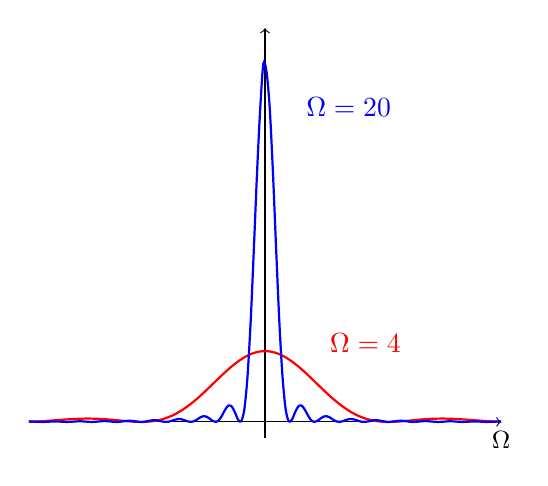
\begin{tikzpicture}
                \draw[->] (-3,0)--(3,0)node[below]{\small\(\Omega\)};
                \draw[->] (0,-0.2)--(0,5);
                \draw[red,thick,domain=-3:3, smooth, variable=\x,samples=50] plot ({\x}, {0.9*sin(2*\x r)*sin(2*\x r)/(4*\x*\x)});
                \draw[blue,thick,domain=-3:3, smooth, variable=\x,samples=150] plot ({\x}, {0.9*sin(10*\x r)*sin(10*\x r)/(20*\x*\x)});
                \node[red] at (0.7,1)[right]{\(\Omega=4\)};
                \node[blue] at (0.4,4)[right]{\(\Omega=20\)};
            \end{tikzpicture}
            \caption{A plot of \(\sin^2\frac{1}{2}\Omega t/\Omega^2 t\) as a function of \(\Omega\). It gets more and more sharply peaked as \(t\to\infty\).}
        \end{figure}

        Therefore, in the \(t\to\infty\) limit, we can write
        \begin{align}
            P_j(t)&=\int\dd{\omega} 2\pi\delta(\omega_{jn}-\omega)\abs{V_{jn}}^2 t\rho(\omega)\notag \\
            &=2\pi\abs{V_{jn}}^2\rho(\omega_{jn})t\,.
        \end{align}
        This is linear in time. The transition rate from \(\ket{n}\) to \(\ket{j}\) is
        \begin{equation}
            R_{nj}=\dv{P_j(t)}{t}=2\pi\abs{V_{jn}}^2\rho(\omega_{jn})\,,
        \end{equation}
        or if we are not using atomic units,
        \begin{equation}
            R_{nj}=\frac{2\pi}{\hbar^2}\abs{V_{jn}}^2\rho(\omega_{jn})\,.
        \end{equation}
        This is \textit{Fermi's golden rule}.

        To move further, we must consider the nature of the \(\hat{V}\) operator. For our purpose, it should describe the interaction between the molecule and the oscillating electric field. The `oscillating' part is already dealt with by the \(\cos\) term in (\ref{EM_Wave_Hamiltonian}), so we need \(\hat{V}\) to be a time-independent operator describing the effect of an electric field of some polarisation (direction) and magnitude, represented by a vector \(\vb{\mathcal{E}}\). We will make some further assumptions:
        \begin{itemize}[topsep=0pt]
            \item The field is continuous. Rigorously, the electromagnetic wave should be quantised into packets of photons, and this is necessary if we want to investigate effects like spontaneous emission. However, this is the realm of quantum field theory, and is far beyond the scope of this course.\footnote{It is fluctuations in the zero-point value of the electromagnetic field that allow the atom to spontaneously emit a photon and decay; heuristically, the fluctuating value of the quantum electromagnetic field --- even in the vacuum --- `tickles' the excited atom prompting the decay. Treating the electromagnetic field classically is appropriate if the radiation comes from a high intensity laser, where the energy density of the field is so high that the stimulated emissions and absorptions dominate. By contrast, emission of light from the atoms in a humble candle is an inherently quantum phenomenon, occurring purely by spontaneous emission once the flame is lit --- candlelight shines even in ambient darkness.}\footnote{Actually, the way you deal with spontaneous emission in QFT is more or less the same as what we have done here. You calculate the transition amplitude from perturbation theory, or more formally Dyson formula that we will introduce in appendix \cref{Chap:Interaction_Picture} \(A\sim\mel{m}{\hat{S}}{n}\). The decay rate is then related to this amplitude by the Fermi's golden rule.}
            \item We assume the amplitude of the field is constant over the molecule. This is known as the \textit{dipole approximation}, and it holds as long as the wavelength of the photon is significantly larger than the size of the molecule, and so it is fine up to UV-Vis spectroscopy. It will be problematic if we are interested in ionisations by X-rays.
            \item We assume that the field is isotropic, so the polarisation can have any random orientation with respect to the molecule.
        \end{itemize}

        Within this approximation, we can write the perturbing Hamiltonian as
        \begin{equation}
            \hat{H}^{(1)}=-\vb{\mathcal{E}}\vdot\hat{\vb{\mu}}\cos(\omega t)\,,
        \end{equation}
        and so
        \begin{equation}
            \hat{V}=-\frac{1}{2}\vb{\mathcal{E}}\vdot\hat{\vb{\mu}}=-\frac{1}{2}\mathcal{E}\hat{\mu}\cos\theta\,,
        \end{equation}
        where \(\theta\) is the angle between the polarising plane of the electromagnetic wave and the dipole moment of the molecule. Note the factor of \(\frac{1}{2}\) comes from (\ref{EM_Wave_Hamiltonian}). Averaging over the angle \(\theta\), we get
        \begin{equation}
            R_{nj}=\frac{\pi}{2\hbar^2}\abs{\mel{j}{\mathcal{E}\vdot\hat{\mu}}{n}}^2\rho(\omega_{jn})\eval{\cos^2\theta}\,,
        \end{equation}
        where
        \begin{equation}
            \eval{\cos^2\theta}=\frac{\int_{0}^{2\pi}\dd{\phi}\int_{0}^{\pi}\dd{\theta}\sin\theta\cos^2\theta}{\int_{0}^{2\pi}\dd{\phi}\int_{0}^{\pi}\dd{\theta}\sin\theta}=\frac{1}{3}\,,
        \end{equation}
        and so
        \begin{equation}
            R_{nj}=\frac{\pi}{6\hbar^2}\mathcal{E}^2\abs{\mel{j}{\hat{\mu}}{n}}^2\rho(\omega_{jn})\,.
        \end{equation}
        The transition dipole moment can only be non-zero if its integrand, \(\psi_j^*\hat{\mu}\psi_n\) is totally symmetric under the operations of the molecule's point group. This requirement restricts the combinations of states between which transitions may be observed, and is the origin of spectroscopic selection rules.

        We have given the transition rate for an individual particle, but we can easily adjust to giving the rate of change of the number of particles in the initial state for a collection of non-interacting particles by multiplying the concentration of particles,
        \begin{equation}
            \dv{n_n}{t}=-\frac{\pi}{6\hbar^2}\mathcal{E}^2\abs{\mel{j}{\hat{\mu}}{n}}^2\rho(\omega_{jn})n_n\,.
        \end{equation}
        This is not quite the same as the expression we saw in A3, this is because there we instead used the energy density of photons, \(\rho'(\nu)\), such that \(\int_{\nu_1}^{\nu_2}\dd{\nu}\rho'(\nu)\) is the energy per unit volume of photons in the frequency range \(\nu_1\) to \(\nu_2\). Here, we defined \(\rho(\omega)\) to be such that \(\int_{\omega_1}^{\omega_2}\dd{\omega}\rho(\omega)\) is the number of particles in the frequency range \(\omega_1\) to \(\omega_2\). Therefore, we need the conversion factor
        \begin{equation}
            \rho(\omega)=\frac{V}{2\pi\hbar\omega}\rho'(\nu)\,.
        \end{equation}
        Also, from Maxwell's equations, we may show that the electric field per photon for a collection of photons in a given volume \(V\) is
        \begin{equation}
            \mathcal{E}=\sqrt{\frac{2\hbar\omega}{\epsilon_0 V}}\,.
        \end{equation}
        Combining all of these together, we get the rate of stimulated absorption
        \begin{equation}
            \dv{n_n}{t}=-B_{nj}\rho'(\nu_{nj})n_n\,,
        \end{equation}
        where the \textit{Einstein \(B\) coefficient is}
        \begin{equation}
            B_{nj}=\frac{1}{6\epsilon_0 \hbar^2}\abs{\mel{j}{\hat{\mu}}{n}}^2=\frac{8\pi^3}{(4\pi\epsilon_0) 3h^2}\abs{\mel{j}{\hat{\mu}}{n}}^2
        \end{equation}
        as claimed in A3: \textit{High Resolution Molecular Spectroscopy}. The same equation also holds for stimulated emissions.
    \end{ex}

    \begin{ex}
        \textit{Dynamic polarisability.}

        We see that near-resonant radiations will induce transition. Let us turn to the response of molecules to oscillating electric fields whose frequency \(\omega\) is far from any transition frequency. To ensure that the molecule is not shocked by the field, we switch it on slowly, with
        \begin{equation}
            \hat{H}^{(1)}=\hat{V}(\ee^{\ii\omega t}+\ee^{-\ii\omega t})(1-\ee^{-kt})=2\hat{V}(1-\ee^{-kt})\cos\omega t\,,
        \end{equation}
        where \(k\ll \omega\). For simplicity, we will assume \(z\) polarised radiation, so that \(\hat{V}=-\frac{1}{2}\hat{\mu_z}\mathcal{E}_z\). Substituting into (\ref{first_order_time_dependent_perturbation}), performing the time integral, and taking the long time limit \(t\gg k^{-1}\), we obtain
        \begin{equation}
            a_j(t)=\frac{1}{2}\mathcal{E}_z\mel{j}{\hat{\mu}_z}{n}\left(\frac{\ee^{\ii(\omega_{jn}+\omega)t}}{\omega_{jn}+\omega}+\frac{\ee^{\ii(\omega_{jn}-\omega)t}}{\omega_{jn}-\omega}\right)\,.
        \end{equation}
        Since our radiation frequency is not close to the energy gaps \(\omega_{jn}\), we don't expect any one of the two terms to dominate, and we have to consider both of them.
        \begin{equation}
            \Psi(t)=\Psi_n(t)+\sum_{j\ne n}a_j(t)\Psi_j(t)\,.
        \end{equation}

        We are interested in how the electron distribution, and hence the electric dipole of the molecule fluctuates in response to the imposed oscillating field, so we would like to evaluate the time-dependent response of the molecular dipole moment.
        \begin{align}
            \mu_z(t)&=\expval{\hat{\mu}_z}{\Psi}\notag\\
            &=\expval{\hat{\mu}_z}{\Psi_n+\sum_{j\ne n}a_j\Psi_j}\notag \\
            &=\mel{\Psi_n}{\hat{\mu}_z}{\Psi_n}+\sum_{j\ne n}[a_j\mel{\Psi_n}{\hat{\mu_z}}{\Psi_j}+a_j^*\mel{\Psi_j}{\hat{\mu}_z}{\Psi_n}]+O(\mathcal{E}_z^2)\notag \\
            &=\expval{\hat{\mu}_z}{n}+\sum_{j\ne n}[a_j\mel{n}{\hat{\mu}_z}{j}\ee^{-\ii\omega_{jn}t}+a_j^*\mel{j}{\hat{\mu}_z}{n}\ee^{\ii\omega_{jn}t}]+O(\mathcal{E}_z^2)\,,
        \end{align}
        where we have kept only the first-order terms in the field strength by discarding contributions that are quadratic in the coefficients \(a_j\).\footnote{The term proportional to \(\mathcal{E}_z^2\) should also have contributions from the second-order perturbation coefficient \(a_j^{(2)}\). We don't have it, so including \(\abs{a_j^{(1)}}^2\) here is meaningless.} Substituting the expression of \(a_j(t)\), we arrive at
        \begin{equation}\label{resonant_dipole}
            \mu_z(t)=\mu_{z,n}^{(0)}+\frac{1}{2}\mathcal{E}_z(\ee^{\ii\omega t}+\ee^{-\ii\omega t})\sum_{j\ne n}\abs{\mel{j}{\hat{\mu}_z}{n}}^2\left(\frac{1}{\omega_{jn}+\omega}+\frac{1}{\omega_{jn}-\omega}\right)\,.
        \end{equation}
        We see that the dipole oscillates harmonically about its permanent value \(\mu_{z,n}^{(0)}\) in the absence of a field with the same frequency \(\omega\) as the driven frequency. Since, in general,
        \begin{equation}
            \mu=-\pdv{E}{\mathcal{E}}=\mu^{(0)}+\alpha\mathcal{E}+\dots\,,
        \end{equation}
        we may interpret the sum in (\ref{resonant_dipole}) as a \textit{frequency-independent} or \textit{dynamic polarisability},
        \begin{equation}\label{dynamic_polarisability}
            \alpha_{zz}(\omega)\coloneqq 2\sum_{j\ne n}\frac{\omega_{jn}\abs{\mel{j}{\hat{\mu}_z}{n}}^2}{\omega_{jn}^2-\omega^2}\,,
        \end{equation}
        so that
        \begin{equation}
            \mu_z(t)=\mu_z^{(0)}+\alpha_{zz}(\omega)\mathcal{E}_z\cos\omega t\,.
        \end{equation}
        The subscript \(zz\) emphasises that it measures the dipole induced in the \(z\) direction by a field along \(z\) direction --- the polarisability is a tensor.

        Note the dynamic polarisability (\ref{dynamic_polarisability}) reduces to the static polarisability (\ref{molecular_polarisability}) as \(\omega\to 0\). Also the polarisability diverges if \(\omega\to\omega_{jn}\) since then an electric dipole will not induce a dipole but instead cause a transition.
    \end{ex}

    \newpage
    \section{Intermolecular Interactions}
    \subsection{The Dispersion Energy}
    Weak attractive forces exist even between uncharged non-polar particles, and are significant enough to result in weakly bound dimers of noble gas atoms. Although atoms are spherical on average, and therefore have no permanent dipole moment, fluctuations in the electron density constitute instantaneous dipole moments. We will show in this section that the average interaction between fluctuations on different atoms lowers the energy, and we will derive an expression for the strength of the resulting \textit{dispersion force}.

    For a two-atom system, A and B, we let the zeroth-order Hamiltonian be the sum of the Hamiltonian of the isolated atoms, and contains no terms of interaction between them:
    \begin{equation}
        \hat{H}^{(0)}=\hat{H}_{\AA}^{(0)}+\hat{H}_{\BB}^{(0)}\,.
    \end{equation}
    The zeroth-order wavefunctions are therefore the products of the individual wavefunctions, \(\psi_{mn}^{(0)}=\psi_{\AA,m}^{(0)}\psi_{\BB,n}^{(0)}\), and we will denote this by \(\ket{mn}\).

    We now add the interaction between the atoms as a perturbation. The largest contribution comes from the energy of the instantaneous dipole moments. From classical electrostatics, and replacing the classical quantities by their quantum mechanical operators, the energy of two point dipole \(\vb{\mu}_{\AA}\) and \(\vb{\mu}_{\BB}\) at separation \(\vb{R}\) is\footnote{Let's put dipole \(\vb{\mu}_{\AA}\) at origin and a dipole \(\vb{\mu}_{\BB}=q\vb{d}\) at \(\vb{R}\), with \(\norm{\vb{R}}\gg\norm{\vb{d}}\). The potential generated by \(\vb{\mu}_{\BB}\) at origin is
    \begin{align}
        \phi&=\frac{1}{4\pi\epsilon_0}\left(\frac{q}{R}-\frac{q}{\norm{\vb{R}+\vb{d}}}\right)\notag\\
        &=\frac{q}{4\pi\epsilon_0}\left[\frac{1}{R}-\left(\frac{1}{R}+\vb{d}\vdot\grad\frac{1}{R}+\frac{1}{2}(\vb{d}\vdot\grad)^2\frac{1}{R}+\dots\right)\right]\notag\\
        &=\frac{q}{4\pi\epsilon_0}\frac{\vb{d}\vdot\vb{R}}{R^3}\notag\\
        &=\frac{\vb{\mu}_{\BB}\vdot\vb{R}}{4\pi\epsilon_0 R^3}\,.
    \end{align}
    Then the electric field by \(\vb{\mu}_{\BB}\) at origin is
    \begin{align}
        \vb{E}&=-\grad\phi=-\frac{1}{4\pi\epsilon_0}\vb{e}_i\pdv{}{x_i}\frac{\mu_{\BB j}x_j}{(x_k x_k)^{3/2}}\notag \\
        &=-\frac{1}{4\pi\epsilon_0}\vb{e}_i\left[\frac{\mu_{\BB j}\delta_{ij}(x_kx_k)^{3/2}-\mu_{\BB j}x_j\cdot\frac{3}{2}(x_l x_l)^{1/2}\cdot 2\delta_{ik}x_k}{(x_m x_m)^{3}}\right]\notag \\
        &=\frac{1}{4\pi\epsilon_0}\vb{e}_i\frac{3(\vb{R}\vdot\vb{\mu}_{\BB})R\vb{R}-\vb{\mu}_{\BB}R^3}{R^6}\notag\\
        &=\frac{\mu_{\BB}}{4\pi\epsilon_0 R^3}[3(\vu{R}\vdot\vu{\mu}_{\BB})\vu{R}-\vu{\mu}_{\BB}]
    \end{align}
    using summation convention. Note a vector with a hat here means unit vector. Then finally, the interaction energy of the two dipoles is
    \begin{equation}
        E=-\vb{E}\vdot\vb{\mu}_{\AA}=\frac{1}{4\pi\epsilon_0 R^3}\left[\vb{\mu}_{\AA}\vdot\vb{\mu}_{\BB}-\frac{3}{R^2}(\vb{R}\vdot\vb{\mu}_{\AA})(\vb{R}\vdot\vb{\mu}_{\BB})\right]\,.
    \end{equation}}
    \begin{equation}
        \hat{H}^{(1)}=\frac{1}{R^3}\left[\hat{\vb{\mu}}_{\AA}\vdot\hat{\vb{\mu}}_{\BB}-\frac{3}{R^2}(\hat{\vb{\mu}}_{\AA}\vdot\vb{R})(\hat{\vb{\mu}}_{\BB}\vdot\vb{R})\right]\,.
    \end{equation}
    Without loss of generality, we can take \(\vb{R}\) to be parallel to \(z\) axis, giving the simpler form
    \begin{equation}
        \hat{H}^{(1)}=\frac{1}{R^3}(\hat{\mu}_{\AA x}\hat{\mu}_{\BB x}+\hat{\mu}_{\AA y}\hat{\mu}_{\BB y}-2\hat{\mu}_{\AA z}\hat{\mu}_{\BB z})\,.
    \end{equation}
    The first-order energy \(E_0^{(1)}=\expval{\hat{H}^{(1)}}{00}\) only contains terms
    \begin{equation}
        \expval{\hat{\mu}_{\AA i}\hat{\mu}_{\BB i}}{00}=\expval{\hat{\mu}_{\AA i}}{0_{\AA}}\expval{\hat{\mu}_{\BB i}}{0_{\BB}}\,,
    \end{equation}
    where \(i\in\{x,y,z\}\). All of these are zero since an atom has no permanent dipole moment in any direction, so \(E_0^{(1)}=0\).

    The second-order energy is
    \begin{equation}\label{dispersion_RS_sum}
        E_0^{(2)}=-\sum_{m\ne 0}\sum_{n\ne 0}\frac{\abs{\mel{00}{\hat{H}^{(1)}}{mn}}^2}{E_{\AA,m}^{(0)}+E_{\BB,n}^{(0)}-E_{\AA,0}^{(0)}-E_{\BB,0}^{(0)}}\,.
    \end{equation}
    Since \(\hat{H}^{(1)}\) contains three terms, the square in the numerator contains nine. However, all the cross terms like
    \begin{equation}
        \mel{00}{\hat{\mu}_{\AA i}\hat{\mu}_{\BB i}}{mn}\mel{mn}{\hat{\mu}_{\AA j}\hat{\mu}_{\BB j}}{00}=\mel{0_{\AA}}{\hat{\mu}_{\AA i}}{m_{\AA}}\mel{0_{\BB}}{\hat{\mu}_{\BB i}}{n_{\BB}}\mel{m_{\AA}}{\hat{\mu}_{\AA j}}{0_{\AA}}\mel{n_{\BB}}{\hat{\mu}_{\BB j}}{0_{\BB}}
    \end{equation}
    vanishes, where \(i\ne j\in\{x,y,z\}\). This is because we can reverse the direction of, say, axis \(i\) on atom \(\AA\), and this will change the sign of the expression. However, energy should be totally symmetric, so it can only be zero. The only non-vanishing terms are
    \begin{equation}
        \mel{00}{\hat{\mu}_{\AA i}\hat{\mu}_{\BB i}}{mn}\mel{mn}{\hat{\mu}_{\AA i}\hat{\mu}_{\BB i}}{00}=\mel{0_{\AA}}{\hat{\mu}_{\AA i}}{m_{\AA}}\mel{0_{\BB}}{\hat{\mu}_{\BB i}}{n_{\BB}}\mel{m_{\AA}}{\hat{\mu}_{\AA i}}{0_{\AA}}\mel{n_{\BB}}{\hat{\mu}_{\BB i}}{0_{\BB}}\,,
    \end{equation}
    where \(i\in\{x,y,z\}\). Moreover, by spherical symmetry, this is the same for \(x\), \(y\) and \(z\), and we have 6 such terms in total (1 from \(x\), 1 from \(y\) and \(2^2=4\) from \(z\)). This gives us the total expression
    \begin{equation}\label{dispersion_force}
        E_0^{(2)}=-\frac{6}{R^6}\sum_{m,n\ne 0}\frac{\abs{\mel{0_{\AA}}{\hat{\mu}_{\AA z}}{m_{\AA}}}^2\abs{\mel{0_{\BB}}{\hat{\mu}_{\BB z}}{m_{\BB}}}^2}{(E_{\AA,m}^{(0)}-E_{\AA,0}^{(0)})+(E_{\BB,n}^{(0)}-E_{\BB,0}^{(0)})}\,.
    \end{equation}
    Since both the numerator and denominator are positive, the dispersion force is attractive and scales as \(R^{-6}\).

    Equation (\ref{dispersion_force}) resembles the polarisability, and we might expect that the strength of dispersion energy would be related to the polarisability of the atom as they need to respond to the instantaneous field generated by each other. However, the connection is not obvious to work out explicitly. We need the seemingly arbitrary identity
    \begin{equation}
        \frac{2}{\pi}\int_{0}^{\infty}\dd{\omega}\frac{xy}{(x^2+\omega^2)(y^2+\omega^2)}=\frac{1}{x+y}\,.\label{an_integral_identity}
    \end{equation}
    Putting \(x=\omega_{m0}=E_{\AA,m}^{(0)}-E_{\AA,0}^{(0)}\) and \(y=\omega_{n0}=E_{\BB,n}^{(0)}-E_{\BB,0}^{(0)}\), the equation becomes
    \begin{align}
        E_0^{(2)}&=-\frac{12}{\pi R^6}\sum_{m,n\ne 0}\int_{0}^{\infty}\dd{\omega}\frac{\omega_{m0}\abs{\mel{0_{\AA}}{\hat{\mu}_{\AA z}}{m_{\AA}}}^2\omega_{n0}\abs{\mel{0_{\BB}}{\hat{\mu}_{\BB z}}{m_{\BB}}}^2}{(\omega_{m0}^2+\omega^2)(\omega_{n0}^2+\omega^2)}\notag\\
        &=-\frac{3}{\pi R^6}\sum_{m,n\ne 0}\int_{0}^{\infty}\dd{\omega}\alpha_{\AA,zz}(\ii\omega)\alpha_{\BB,zz}(\ii\omega)\,,\label{dispersion_force_dynamic_polarisability}
    \end{align}
    where
    \begin{equation}\label{dynamic_polarisability_imaginary_frequency}
        \alpha_{zz}(\ii\omega)=2\sum_{n\ne 0}\frac{\omega_{n0}\abs{\mel{0}{\hat{\mu}_z}{n}}^2}{\omega_{n0}^2+\omega^2}
    \end{equation}
    is the dynamic polarisability (\ref{dynamic_polarisability}) with imaginary frequency. 

    The advantage of (\ref{dispersion_force_dynamic_polarisability}) is that it is formally exact and of practical use, since the polarisabilities can be calculated both experimentally and computationally. The dispersion energy is often written \(-C_6/R^6\), where the coefficient \(C_6\) is often treated as an empirical quantity. \Cref{dispersion_force_dynamic_polarisability}, however, allows us to compute it analytically.

    \subsubsection{Drude--London Model (Non-examinable)}
    The dispersion interaction (\ref{dispersion_force_dynamic_polarisability}) simplifies to some even simpler form if we are willing to take further approximations. London claimed that our expansion of dynamic polarisability with imaginary frequency (\ref{dynamic_polarisability_imaginary_frequency}) can be approximated by a single term
    \begin{equation}
        \alpha(\ii\omega)\approx\frac{2\omega_0\abs{\mu_{\text{eff}}}^2}{\omega_0^2+\omega^2}\,,
    \end{equation}
    where \(\omega_0\) sits somewhere near the ionisation threshold of the atom,
    \begin{equation}
        \omega_0\simeq I\,.
    \end{equation}
    The static polarisability is then obtained by taking \(\omega=0\) (or by doing the same approximation to (\ref{RS_polarisability_expansion}))
    \begin{equation}
        \alpha(0)\approx\frac{2\abs{\mu_{\text{eff}}}^2}{\omega_0}\,.
    \end{equation}
    This allows us to write
    \begin{equation}
        \alpha(\ii\omega)=\frac{\alpha(0)\omega_0^2}{\omega_0^2+\omega^2}\,.
    \end{equation}
    This is the \textit{Drude--London model}.\footnote{It seems that we have done some crazy approximations that makes little sense, but there are some rationalisation for this. If you have a classical Lorentz oscillator of charge \(q\), mass \(m\) and natural frequency \(\omega_0\) driven at imaginary frequency \(\ii\omega\), the equation of motion
    \begin{equation}
        m\ddot{x}+m\omega_0^2 x=qE_0\ee^{\ii\omega t}
    \end{equation}
    gives
    \begin{equation}
        \alpha(\ii\omega)=\frac{q^2/m}{\omega_0^2+\omega^2}=\frac{\alpha(0)\omega_0^2}{\omega_0^2+\omega^2}\,,
    \end{equation}
    where \(\alpha(0)=q^2/m\omega_0^2\). Another rationalisation is the sum-rule (Slater--Kirkwood) matching, which is a lot more complicated, and we will not explain it here.} Plugging this into the integral (\ref{dispersion_force_dynamic_polarisability}) gives
    \begin{equation}
        E_0^{(2)}=-\frac{3}{\pi R^6}\int_{0}^{\infty}\dd{\omega}\frac{\alpha_{\AA}(0)\alpha_{\BB}(0)\omega_{\AA 0}^2\omega_{\BB 0}^2}{(\omega_{\AA 0}^2 +\omega^2)(\omega_{\BB 0}^2 +\omega^2)}\,.
    \end{equation}
    We can invoke the integral identity (\ref{an_integral_identity}) again to get
    \begin{align}
        E_0^{(2)}&=-\frac{3}{2}\frac{\omega_{\AA 0}\omega_{\BB 0}}{\omega_{\AA 0} + \omega_{\BB 0}}\frac{\alpha_{\AA}(0)\alpha_{\BB}(0)}{R^6}\notag\\
        &=-\frac{3}{2}\frac{I_{\AA}I_{\BB}}{I_{\AA} + I_{\BB}}\frac{\alpha_{\AA}(0)\alpha_{\BB}(0)}{R^6}
    \end{align}

    \subsection{The Induction Energy}
    The situation would be much more complex for molecules. If the molecule possesses a permanent dipole, then the first-order energy
    \begin{equation}
        E_0^{(1)}=\expval{\hat{H}^{(1)}}{00}\,,
    \end{equation}
    where
    \begin{equation}
        E_0^{(1)}=\frac{1}{R^3}(\mu_{\AA x}^{(0)}\mu_{\BB x}^{(0)}+\mu_{\AA y}^{(0)}\mu_{\BB y}^{(0)}-2\mu_{\AA z}^{(0)}\mu_{\BB z}^{(0)})\,,
    \end{equation}
    is no longer zero. But since the interaction is now orientation-dependent, we need to integrate over all possible relative orientations weighted by the corresponding Boltzmann factor since not all orientations are equally probable and obtain a weighted average of interaction. This is too complicated to deal with, so we will not do it here. We will quote the result:
    \begin{equation}
        \eval{E_0^{(1)}}=-\frac{\mu_{\AA}^2\mu_{\BB}^2}{k_B TR^3}\,.
    \end{equation}
    This is the thermal average of the interaction energy between two isolated dipoles, scaling as \(R^{-3}\).\footnote{This is not what happens in a bulk system where there are more than just two molecules. When interaction strengths \(\ll k_B T\), the orientations of the molecules would be isotropic, and this first order contribution will also vanish as there will be on average as many alignment as misalignments of molecular orientations. In such case, the average interaction between each pair of molecules would be
    \begin{equation}
        -\frac{\mu_\AA^2\mu_\BB^2}{3k_B T R^6}\,,
    \end{equation}
    which again scales as \(R^{-6}\). This is known as the \textit{Keesom interaction}.}

    In the second-order energy, we should only exclude \(\ket{m,n}=\ket{0,0}\) from the Rayleigh--Schr\"{o}dinger sum, but in the dispersion force of atom, (\ref{dispersion_RS_sum}), we have excluded all states with either \(m=0\) or \(n=0\) since they evaluate to zero. The dispersion energy can be thought of as an interaction between simultaneous excited states of two atoms. However, for polar molecules, terms of form \(\mel{00}{\hat{H}^{(1)}}{m0}\) and \(\mel{00}{\hat{H}^{(1)}}{0n}\), where only one of the two species is excited, may be non-zero. It is therefore conventional to separate the second-order energy into three contributions,
    \begin{equation}
        E_0^{(2)}=E_{\text{disp}}+E_{\AA,\text{ind}}+E_{\BB,\text{ind}}\,,
    \end{equation}
    where
    \begin{align}
        E_{\text{disp}}&=-\sum_{m\ne 0}\sum_{n\ne 0}\frac{\abs{\mel{00}{\hat{H}^{(1)}}{mn}}^2}{E_{\AA,m}^{(0)}+E_{\BB,n}^{(0)}-E_{\AA,0}^{(0)}-E_{\BB,0}^{(0)}}\,, \label{molecular_dispersion}\\
        E_{\AA,\text{ind}}&=-\sum_{m\ne 0}\frac{\abs{\mel{00}{\hat{H}^{(1)}}{m0}}^2}{E_{\AA,m}^{(0)}-E_{\AA,0}^{(0)}}\,, \label{molecular_induction_A} \\
        E_{\BB,\text{ind}}&=-\sum_{n\ne 0}\frac{\abs{\mel{00}{\hat{H}^{(1)}}{0n}}^2}{E_{\BB,n}^{(0)}-E_{\BB,0}^{(0)}}\,.\label{molecular_induction_B}
    \end{align}
    The dispersion term (\ref{molecular_dispersion}) is again the interaction between the instantaneous dipole of \(\AA\) and the instantaneous dipole of \(\BB\), but we now have two extra contributions. The induction terms (\ref{molecular_induction_A}) and (\ref{molecular_induction_B}) are the interactions between permanent dipole of \(\AA\) with the instantaneous dipole of \(\BB\), and the permanent dipole of \(\BB\) with the instantaneous dipole of \(\AA\), respectively.\footnote{In bulk system, the orientationally averaged induction interaction becomes what is known as the \textit{Debye force}. For a polar molecule A and non-polar molecule B, the interaction energy is given by
    \begin{equation}
        -\frac{\mu_\AA^2\alpha_B}{R^6}\,.
    \end{equation}
    Note that it also scales as \(R^{-6}\), and it is now temperature independent.}

    \newpage
 
    \section{Relativistic Effects}
    Everything we discussed so far ignores \textit{relativity}, which refers to the breakdown of non-relativistic mechanics when particles have relative speeds approaching the speed of light in vacuum. Special relativity is the simpler theory of relativity, which deals with situations in which gravity is negligible. This is almost always the case as far as chemistry is concerned since electromagnetic forces are orders of magnitude larger than gravity.\footnote{The electromagnetic force between two electrons can be written as a power series in the dimensionless \textit{fine structure constant}, \(\alpha\approx\frac{1}{137}\), which characterises the strengths of electromagnetic forces. The corresponding parameter characterising the strength of gravitational force is \(\alpha_{\text{G}}\sim 10^{-45}\), which is much smaller. It is therefore always safe to ignore gravitational interactions in chemical systems.} The incorporation of special relativity into quantum mechanics is known as \textit{Quantum Field Theory} (QFT), and it was first achieved by Dirac in 1927. As its name suggests, quantum field theory is the quantisation of the classical field theory, in which all the fields, such as the electromagnetic field, are being quantised. Moreover, elementary particles like electrons are also thought of as `ripples' on an `electron field' spanning throughout the whole universe. This is a much deeper subject, but it can be chemically significant --- in particular, spontaneous emission can only be explained by QFT.\footnote{If you are really interested in QFT (I hope you are not), you can check Prof. David Tong's notes on Quantum Field Theory, which is a Part III course for Mathematical Tripos. It takes him 4 chapters to arrive at Dirac's equation, and to have a firm grasp on it, you should probably also read his notes on Classical Dynamics and General Relativity as prerequisites.}
    
    General relativity is much more complicated and the unification of quantum mechanics and general relativity (known as quantum gravity) is still an important open question in theoretical physics.

    Although chemists often ignore relativity, as you have previously seen in the IA inorganic and materials chemistry course, relativistic effects are significant for heavy atoms. However, any sufficiently precise prediction for any atom, including hydrogen, must include relativistic effects to be accurate.

    The \textit{Dirac equation}, in the form originally proposed by Dirac, for a free electron is
    \begin{equation}
        \left(\beta m_e c^2 + c\sum_{n=1}^{3}\alpha_n\hat{p}_n\right)\vb{\psi}(\vb{x},t)=\ii\hbar\pdv{\psi(\vb{x},t)}{t}\,.
    \end{equation}
    You can find a brief derivation of Dirac equation in \cref{Chap:Dirac_eqn}. This looks reminiscent to the time-dependent Schr\"{o}dinger equation, but with a few important differences. The wavefunction \(\vb{\psi}\) is no longer a scalar function, but a 4-component vector\footnote{Technically, a \textit{bispinor}. It transforms in a slightly different way than vectors under rotation.}, which corresponds to a spin-up and spin-down electron, and a spin-up and spin-down positron. The operator in brackets on the left replaces the non-relativistic Hamiltonian. \(\alpha_n\) and \(\beta\) are \(4\times 4\) matrices that obey certain symmetry and commutation properties. \(m_e\) is the rest mass of the electron, \(c\) is the speed of light and \(\hat{p}_n\) is the \(n^{\text{th}}\) component of the momentum operator. To include the potential due to the hydrogen nucleus, we add in the potential term
    \begin{equation}
        \left(\beta m_e c^2 + c\sum_{n=1}^{3}\alpha_n\hat{p}_n-\frac{e^2}{4\pi\epsilon_0 r}\right)\vb{\psi}(\vb{x},t)=\ii\hbar\pdv{\psi(\vb{x},t)}{t}\,.
    \end{equation}
    The Dirac equation for free spin-\(\frac{1}{2}\) massive particle is often recast in a more compact form as
    \begin{equation}
        \left(\ii\hbar\gamma^\mu\hat{\partial}_\mu-mc\right)\vb{\psi}=\vb{0}\,,
    \end{equation}
    where \(\gamma^\mu\) is a set of \(4\times 4\) matrices formed from \(\alpha_n\) and \(\beta\), known as the \textit{Dirac (gamma) matrices}. \(\hat{\partial}_{\mu}\) is the component of the 4-gradient (essentially \(\grad\) with an extra zeroth dimension of time), and Einstein summation applies to sum over the four components \(\mu\).

    As gravity is completely negligible in chemical systems, exact solutions to the Dirac equation offer a huge improvement over the non-relativistic Schr\"{o}dinger equation. However, we already know that the exact solutions to the Schr\"{o}dinger equation are rare for chemical systems, the Dirac equation is only even harder to deal with.

    This leads to the famous claim of Paul Dirac.
    \begin{quote}
        ``The underlying physical laws necessary for the mathematical theory of a large part of physics and the whole of chemistry are thus completely known, and the difficulty is only that the exact application of these laws leads to equations much too complicated to be soluble.''

        \hfill --- Paul Dirac (1929), \textit{The quantum mechanics of many-electron systems.}
    \end{quote}

    Since Dirac's claim, significant progress has been made in the field of numerical solutions, particularly with the advent of fast digital computation, and it is no longer the case that Dirac's equation is too complicated to be (numerically) solvable. It is, however, still complicated to be soluble using pen and paper.

    Instead, to investigate the relativistic effect, we will use perturbation theory to add the terms that arise from the non-relativistic limit of Dirac's equation into Schr\"{o}dinger equation as small perturbations. Our main example would be hydrogen spectrum, the observations of which were also historically a significant driver in the development of relativistic quantum mechanics.

    \subsection{Hydrogen Fine Structure}
    The \textit{Lyman-\(\alpha\) line} in the hydrogen spectrum is the \(n=1\to 2\) transition observed at around \(121.57\unit{nm}\). Using the familiar exact solution to the Schr\"{o}dinger equation, we can predict that the line should be observed at
    \begin{equation}
        h\nu=E_2-E_1=R_{\mathrm{H}}\left(1-\frac{1}{4}\right)=\frac{3}{4}R_{\mathrm{H}}\,,
    \end{equation}
    where \(R_{\mathrm{H}}\) is the Rydberg constant.

    There is actually a subtlety concerning this constant that is worth mentioning. The collection of constants that emerge from the normal Schr\"{o}dinger equation for the Rydberg constant is
    \begin{equation}
        R_\infty=\frac{m_e e^4}{8\epsilon_0^2 h^2}=2.179\,87\times 10^{-18}\unit{J}\,.
    \end{equation}
    Using this value, we will predict the Lyman-\(\alpha\) line should appear at \(121.50\unit{nm}\), noticeably different from the experimental value. The error arises from the Born--Oppenheimer approximation: we have treated the nucleus as immobile, or equivalently having infinite mass (and hence the subscript \(\infty\) in the Rydberg constant). The hydrogen nucleus is indeed massive compared with the electron, but it is only heavier by a factor of \(\sim 1836\). The error of this approximation is easily observable in accurate spectroscopic measurement. Instead, we should replace the electron mass with the reduced mass of the electron-proton system
    \begin{equation}
        \mu=\frac{m_e m_p}{m_e+m_p}\approx 0.999\,455\, m_e\,,
    \end{equation}
    which gives the true Rydberg constant
    \begin{equation}
        R_{\mathrm{H}}=\frac{\mu e^4}{8\epsilon_0^2 h^2}=2.178\,69\times 10^{-18}\unit{J}\,.
    \end{equation}
    Using this value, we predict the Lyman-\(\alpha\) line at \(121.57\unit{nm}\), in agreement with experiment. Incidentally, this also implies that the line for deuterium should be at a slightly shorter wavelength than hydrogen due to a slightly larger effective mass, appearing at \(121.54\unit{nm}\). This is actually how the existence of deuterium was proved in 1931, surprisingly even slightly before the discovery of neutron in 1932.

    Even in the late nineteenth century, the precision of UV spectrometers exceeds the one-hundredth of a \(\mathrm{nm}\) we have just quoted. This reveals some more surprising details in the hydrogen energy levels. In 1887, after Michelson and Morley failed to detect ether drift using their high precision interferometer, they turned their eye to investigate atomic spectra. They found that the hydrogen spectral lines were not singlets as predicted by Schr\"{o}dinger equation, but actually consisted of closely spaced multiple components. This splitting, which is also later observed for other atomic spectra, is called the \textit{fine structure} of the spectrum. For example, Theodore Lyman observed that the Lyman-\(\alpha\) for hydrogen is split into a doublet, with lines at \(121.5668\unit{nm}\) and \(121.5674\unit{nm}\). The fine structure is a result of relativistic effects, and we will have a look at how relativity give rise to it.

    \begin{figure}
        \centering
        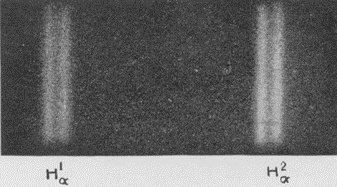
\includegraphics[width=0.5\textwidth]{Hydrogen_fine_structure.png}
        \caption{\(\mathrm{H}_\alpha\) (\(n=2\to n=3\)) lines of hydrogen and deuterium. Each is shown to be a doublet. Figure adapted from G.N. Lewis and F.H. Spedding, Phys. Rev. 43, 964 (1933).}
    \end{figure}

    \subsubsection{Relativistic Kinetic Energy}
    The first relativistic contribution is the easiest to understand. It arises from the relativistic correction to the kinetic energy. Classically, the non-relativistic kinetic energy is
    \begin{equation}
        T=\frac{\vb{p}^2}{2m}\,,
    \end{equation}
    where \(\vb{p}=m\vb{v}\) is the classical non-relativistic momentum. However, in special relativity, the kinetic energy is given by
    \begin{equation}
        T=(\gamma-1)mc^2\,.
    \end{equation}
    Written in terms of the (relativistic) canonical momentum \(p\), this is
    \begin{align}
        T&=\sqrt{\vb{p}^2 c^2+m^2 c^4}-mc^2\notag\\
        &=mc^2\left(\sqrt{1+\frac{\vb{p}^2}{m^2c^2}}-1\right)\,.
    \end{align}

    Expanding for \(\abs{\vb{p}}\ll mc\) gives\footnote{Here \(\vb{p}\) denotes the relativistic canonical momentum, represented in QM by \(-\ii\hbar\grad\). In the non-relativistic limit this coincides with \(m\vb{v}\), but in the relativistic regime \(\vb{p}=\gamma m\vb{v}\). That is why we expand \(T\) in powers of relativistic momentum \(\vb{p}\) rather than non-relativistic momentum \(m\vb{v}\).}
    \begin{equation}
        T=\frac{\vb{p}^2}{2m}-\frac{\vb{p}^4}{8m^3 c^2}+\dots
    \end{equation}
    The first term is just the non-relativistic kinetic energy, and the second term is the relativistic correction to the leading order. Therefore, for a hydrogen atom, we use perturbative Hamiltonian\footnote{The official handout is again being rather loose here and directly set \(\mu=m_e=1\) in atomic units.}
    \begin{equation}
        \hat{H}_{T}^{(1)}=-\frac{\hat{\vb{p}}^4}{8\mu^3 c^2}\,.
    \end{equation}
    This term is the first of our three relativistic corrections, and we use a subscript \(T\) to stand for the kinetic contribution to the relativistic correction. The first-order perturbation to the energy is\footnote{One might be worrying about the degeneracies. Note that our system is rotationally invariant, so in particular \([L_z,\hat{H}_{T}^{(1)}]=0\) and \([\vb{L}^2,\hat{H}_{T}^{(1)}]=0\). Therefore \(\mel{n,\ell',m'}{\hat{H}_{T}^{(1)}}{n,\ell,m}=0\) unless both \(\ell'=\ell\) and \(m'=m\). Thus our perturbation does not mix degenerate states of the gross structure, so non-degenerate perturbation theory is sufficient.}
    \begin{equation}
        E_{T,n\ell m}^{(1)}=\expval{\hat{H}_T^{(1)}}{n,\ell,m}=-\frac{1}{8\mu^3 c^2}\expval{\hat{\vb{p}}^4}{n,\ell,m}\,.
    \end{equation}
    We can obtain a general expression of this by some algebraic manipulations. The Schr\"{o}dinger equation of the reference Hamiltonian gives
    \begin{align}
        \left(\frac{\hat{\vb{p}}^2}{2\mu}-\frac{1}{r}\right)\ket{n,\ell,m}&=E_n^{(0)}\ket{n,\ell,m}\\
        \hat{\vb{p}}^2\ket{n,\ell,m}&=2\mu\left(\frac{1}{r}+E_n^{(0)}\right)\ket{n,\ell,m}
    \end{align}
    in atomic units, where \(E_n^{(0)}=-\frac{\mu}{2n^2}\) is the non-relativistic energy of state \(\ket{n,\ell,m}\) of hydrogen atom.\footnote{You might be more familiar with the energy \(E_n^{(0)}=-\frac{1}{2n^2}\), but this is under Born--Oppenheimer approximation.} Therefore,
    \begin{align}
        E_{T,n\ell m}^{(1)}&=-\frac{1}{8\mu^3 c^2}\expval{\hat{\vb{p}}^2\hat{\vb{p}}^2}{n,\ell,m}\notag\\
        &=-\frac{1}{2\mu c^2}\left(\frac{\mu^2}{4n^4}-\frac{\mu}{n^2}\eval{\frac{1}{r}}+\eval{\frac{1}{r^2}}\right)\,.
    \end{align}
    For hydrogen orbital, it can be shown that\footnote{The first result is obvious from the virial theorem, which states that for a potential \(V(r)=ar^k\), we have \(2\eval{T}=k\eval{V}\), and so for the Coulomb potential, \(\eval{\frac{1}{r}}=-\eval{V}=-2E_n^{(0)}\). The second result can also be evaluated using some tricks of defining an effective potential. See my notes on Principles of Quantum Mechanics.}
    \begin{align}
        \eval{\frac{1}{r}}&=\frac{\mu}{n^2}\,,\\
        \eval{\frac{1}{r^2}}&=\frac{\mu^2}{n^3\left(\ell+\frac{1}{2}\right)}\,.
    \end{align}
    Combining all these, we get
    \begin{equation}
        E_{T,n\ell m}^{(1)}=-\frac{\mu}{8n^4 c^2}\left(\frac{4n}{\ell+\frac{1}{2}}-3\right)\,.
    \end{equation}

    \subsubsection{Spin-Orbit Coupling}
    Due to its spin, an electron has a magnetic dipole moment. Since the electron is moving around the nucleus, from the perspective of the electron, the nucleus is also moving around the electron, so the electron is effectively experiencing a magnetic field. The magnetic dipole moment of the electron can interact with the magnetic field, and the Hamiltonian of this perturbation is\footnote{The magnetic dipole moment of the electron is given by
    \begin{equation}
        \vb{m}=-\frac{g_s}{2\mu}\vb{s}\,,
    \end{equation}
    where \(g_s\) is the electron \(g\) factor. It is exactly 2 in Dirac's theory, but in quantum field theory (and in reality), it takes the value \(g_s\approx 2.002\,319\dots\) due to an effect called anomalous magnetic dipole moment. When placed in a magnetic field, this magnetic dipole will have an energy \(U=-\vb{m}\vdot\vb{B}\). If the electron has velocity \(\vb{v}=\vb{p}/\mu\gamma\), then classically the Lorentz transformation of the electric field generated by the nucleus gives the magnetic field experienced by the electron
    \begin{equation}
        \vb{B}=\frac{\gamma}{c^2}\vb{v}\cross\vb{E}=\frac{1}{\mu c^2}\vb{p}\cross\left(-\frac{\vu{r}}{r^2}\right)=\frac{1}{\mu c^2 r^3}\vb{l}\,.
    \end{equation}
    This contributes
    \begin{equation}
        \frac{g_s}{2\mu^2 c^2}\frac{\vb{l}\vdot\vb{s}}{r^3}
    \end{equation}
    to the energy, and is known as the Larmor interaction. There is another complicated effect called Thomas precession, which reduces the energy by \(\vb{l}\vdot\vb{s}/2\mu^2c^2r^3\). Therefore, the total interaction energy is
    \begin{equation}
        U=\frac{(g_s-1)}{2\mu^2c^2r^3}\vb{l}\vdot\vb{s}\approx \frac{1}{2\mu^2c^2r^3}\vb{l}\vdot\vb{s}
    \end{equation}
    using the approximate value \(g_s=2\) (ignoring QFT effects).}
    \begin{equation}
        \hat{H}_{\text{SO}}^{(1)}=\frac{1}{2\mu^2 c^2}\frac{\hat{\vb{l}}\vdot\hat{\vb{s}}}{r^3}\,,
    \end{equation}
    and so the first-order change in the energy is
    \begin{equation}
        E_{\text{SO},n\ell m}^{(1)}=\frac{1}{2\mu^2c^2}\eval{\hat{\vb{l}}\vdot\hat{\vb{s}}}\eval{\frac{1}{r^3}}\,.
    \end{equation}
    We have\footnote{This can also be calculated using effective potential. See Principles of Quantum Mechanics.}
    \begin{equation}
        \eval{\frac{1}{r^3}}=\frac{\mu^3}{n^3\ell(\ell+\frac{1}{2})(\ell+1)}\,.
    \end{equation}
    Next, to evaluate the spin-orbit expectation, we introduce the total angular momentum operator \(\hat{\vb{\jmath}}=\hat{\vb{l}}+\hat{\vb{s}}\). The reference wavefunctions are eigenfunctions of \(\hat{\vb{l}}^2\) and \(\hat{\vb{s}}^2\) with eigenvalues \(\ell(\ell+1)\) and \(s(s+1)=\frac{3}{4}\) respectively, and are also eigenfunctions of \(\hat{\vb{\jmath}}^2\) with eigenvalues \(j(j+1)\). \(j\) is the quantum number for the magnitude of the total angular momentum with possible values given by the Clebsch--Gordan series
    \begin{equation}
        j\in\{\ell+s,\ell+s-1,\dots,\abs{\ell-s}\}\,.
    \end{equation}
    Since \(s=\frac{1}{2}\), the series reduces to
    \begin{equation}
        j=\begin{cases}
            \ell\pm\frac{1}{2} & \ell\ne 0 \\
            \frac{1}{2} & \ell =0
        \end{cases}\,.
    \end{equation}
    Since
    \begin{equation}
        \eval{\hat{\vb{\jmath}}^2}=\eval{(\hat{\vb{l}}+\hat{\vb{s}})^2}=\eval{\hat{\vb{l}}^2}+\eval{\hat{\vb{s}}^2}+2\eval{\hat{\vb{l}}\vdot\hat{\vb{s}}}\,,
    \end{equation}
    we have
    \begin{align}
        \eval{\hat{\vb{l}}\vdot\hat{\vb{s}}}&=\frac{1}{2}\left(\eval{\hat{\vb{\jmath}}^2}-\eval{\hat{\vb{l}}^2}-\eval{\hat{\vb{s}}^2}\right)\notag \\
        &=\frac{1}{2}\left(j(j+1)-\ell(\ell+1)-\frac{3}{4}\right)\,.
    \end{align}
    Putting these together, we have the spin-orbit coupling energy
    \begin{equation}\label{spin_orbit_coupling}
        E_{\text{SO},n\ell m;j}^{(1)}=\frac{\mu}{4c^2}\frac{j(j+1)-\ell(\ell+1)-\frac{3}{4}}{n^3\ell(\ell+\frac{1}{2})(\ell+1)}\,.
    \end{equation}

    \subsubsection{The Darwin Term}
    The third relativistic term is the Darwin term\footnote{This is due to Charles Galton Darwin (1887-1962), not the more famous Charles Robert Darwin (1809-1882).} and is somewhat more mysterious in origin. It has various interpretations, including a small rapid oscillation of the electron (\textit{zitterbewegung}) near the nucleus, a small mixing with the positron component of the wavefunction, or the effect of spontaneously appearing and annihilating electron-positron pairs. Regardless of the origin, it is a perturbation to the potential energy and has the form
    \begin{equation}
        \hat{H}_{\text{D}}^{(1)}=\frac{\pi}{2\mu^2 c^2}\delta^{(3)}(\vb{r})\,,
    \end{equation}
    where \(\delta^{(3)}(\vb{r})\) is the 3D Dirac delta. Since it only picks out the value of a function at the origin in an integral, only orbitals non-zero at the origin will be affected, which is only the \(s\) orbitals. For \(\ell\ne 0\), the first-order energy is zero. For \(s\) orbitals, the values of their wavefunctions at origin are
    \begin{equation}
        \psi_{n00}^{(0)}(\vb{0})=\sqrt{\frac{\mu^3}{n^3\pi}}\,,
    \end{equation}
    giving a Darwin contribution
    \begin{equation}
        E_{\text{D},n\ell m}=\frac{\pi}{2\mu^2 c^2}\abs{\psi_{n00}^{(0)}(\vb{0})}^2\delta_{\ell 0}=\frac{\mu}{2c^2n^3}\delta_{\ell 0}\,.
    \end{equation}

    \subsubsection{Total Effect}
    If we combine the three first-order relativistic corrections for hydrogen, we get the total expression
    \begin{align}
        E_{nj}^{(1)}&=E_{\text{T}}^{(1)}+E_{\text{SO}}^{(1)}+E_{\text{D}}^{(1)}\notag \\
        &=-\frac{\mu}{2c^2n^4}\left(\frac{n}{j+\frac{1}{2}}-\frac{3}{4}\right)\notag \\
        &=\frac{E_n^{(0)}}{c^2 n^2}\left(\frac{n}{j+\frac{1}{2}}-\frac{3}{4}\right)\,.\label{fine_structure}
    \end{align}
    Note that the \(\ell\)-dependence has magically disappeared, and the energy is now only dependent on \(n\) and \(j\). The first order energy here is always negative, so the relativistic correction is a decrease in energy.

    As with much of spectroscopy, measurements and fitting were carried out before the theory had existed to explain the observations. For historical reasons, (\ref{fine_structure}) is often written as
    \begin{equation}
        E_{nj}^{(1)}=\frac{E_n^{(0)}\alpha^2}{n^2}\left(\frac{n}{j+\frac{1}{2}}-\frac{3}{4}\right)\,,
    \end{equation}
    where \(\alpha\) is the \textit{fine-structure constant}. In atomic units, it is
    \begin{equation}
        \alpha=\frac{1}{c}\approx\frac{1}{137}\,.
    \end{equation}
    Since \(\alpha\) is dimensionless, it is the same number in real units
    \begin{equation}
        \alpha=\frac{e^2}{4\pi\epsilon_0\hbar c}\approx\frac{1}{137}\,.
    \end{equation}

    We can now calculate the magnitudes of the relativistic corrections to the hydrogen energy levels \(n=1\) and \(n=2\) and predict the observed fine-structure for the Lyman-\(\alpha\) line. Using the expressions derived above, we predict the two Lyman-\(\alpha\) lines to be spaced by \(0.54\unit{pm}\) in wavelength. The experimental value is \(0.60\unit{pm}\). We have accounted for a large proportion of this shift.

    \begin{figure}
        \centering
        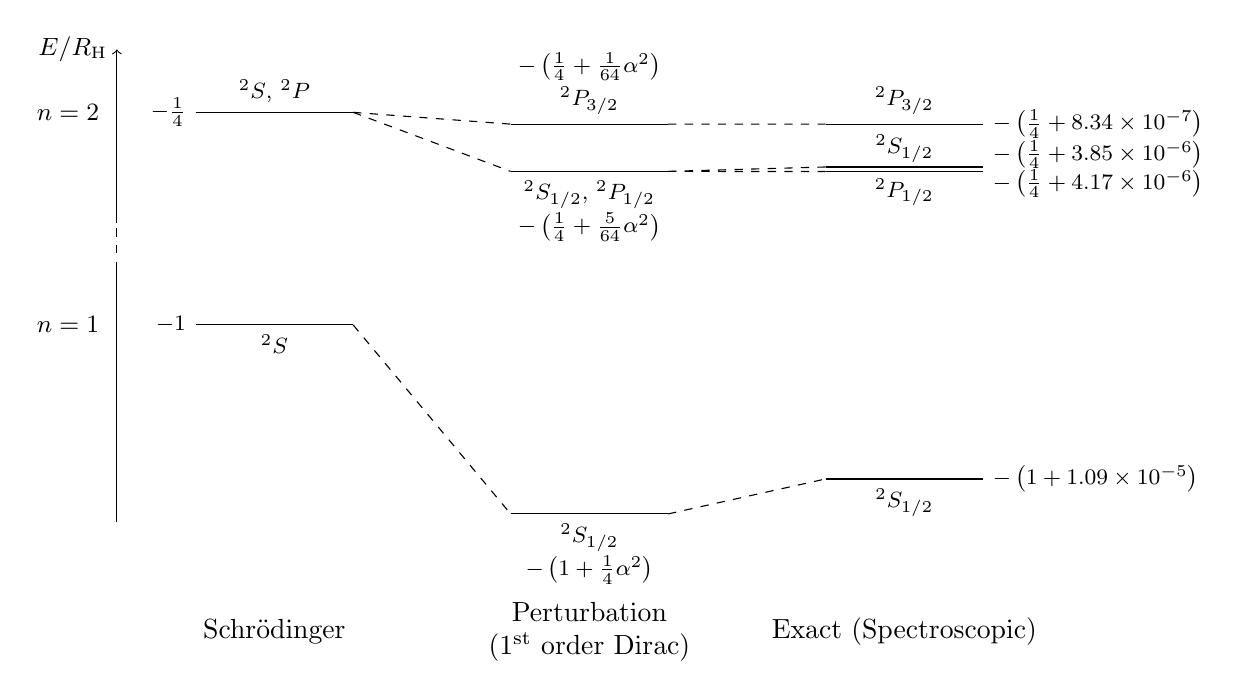
\begin{tikzpicture}
            \draw (0,-1)--(0,2.2);
            \draw[dashed] (0,2.2)--(0,2.8);
            \draw[->] (0,2.8)--(0,5)node[left]{\small\(E/R_{\mathrm{H}}\)};

            \node at (0,1.5)[left=0.1cm]{\small\(n=1\)};
            \node at (0,4.2)[left=0.1cm]{\small\(n=2\)}; 

            \draw (1,1.5)node[left]{\footnotesize \(-1\)}--node[below]{\footnotesize\(^2 S\)}(3,1.5);
            \draw (1,4.2)node[left]{\footnotesize \(-\frac{1}{4}\)}--node[above]{\footnotesize\(^2 S\), \(^2 P\)}(3,4.2);

            \draw[dashed] (3,1.5)--(5,-0.9);
            \draw[dashed] (3,4.2)--(5,3.45);
            \draw[dashed] (3,4.2)--(5,4.05);

            \draw (5,-0.9)--node[below,align=center]{\footnotesize\(^2 S_{1/2}\)\\\footnotesize \(-\left(1+\frac{1}{4}\alpha^2\right)\)}(7,-0.9);
            \draw (5,3.45)--node[below,align=center]{\footnotesize\(^2 S_{1/2}\), \(^2P_{1/2}\)\\\footnotesize \(-\left(\frac{1}{4}+\frac{5}{64}\alpha^2\right)\)}(7,3.45);
            \draw (5,4.05)--node[above,align=center]{\footnotesize \(-\left(\frac{1}{4}+\frac{1}{64}\alpha^2\right)\)\\\footnotesize \(^2P_{3/2}\)}(7,4.05);

            \draw[dashed] (7,-0.9)--(9,-0.456);
            \draw[dashed] (7,3.45)--(9,3.506);
            \draw[dashed] (7,3.45)--(9,3.448);
            \draw[dashed] (7,4.05)--(9,4.0496);

            \draw (9,-0.456)--node[below]{\footnotesize\(^2 S_{1/2}\)}(11,-0.456)node[right]{\footnotesize \(-\left(1+1.09\times 10^{-5}\right)\)};
            \draw (9,3.448)--node[below=-1pt]{\footnotesize\(^2P_{1/2}\)}(11,3.448);
            \draw (9,3.506)--node[above=-2pt]{\footnotesize\(^2S_{1/2}\)}(11,3.506);
            \node at (11,3.478)[right,align=center]{\footnotesize \(-\left(\frac{1}{4}+3.85\times 10^{-6}\right)\) \\[-1.5pt] \footnotesize \(-\left(\frac{1}{4}+4.17\times 10^{-6}\right)\)};
            \draw (9,4.0496)--node[above]{\footnotesize\(^2 P_{3/2}\)}(11,4.0496)node[right]{\footnotesize \(-\left(\frac{1}{4}+8.34\times 10^{-7}\right)\)};

            \node at (2,-2.4) {Schr\"{o}dinger};
            \node at (6,-2.4)[align=center] {Perturbation \\ (\(1^{\text{st}}\) order Dirac)};
            \node at (10,-2.4) {Exact (Spectroscopic)};
        \end{tikzpicture}
        \caption{The relativistic and non-relativistic pictures of the hydrogen energy levels. The graph is to scale, only with the huge spacing between the \(n=1\) and \(n=2\) levels shortened --- otherwise this gap alone would span roughly 4500 pages at this scale. The fine structure is indeed a tiny effect!}
    \end{figure}

    There are many remaining sources of error. The exact solution of Dirac's equation for a hydrogenic atom gives
    \begin{equation}
        E_{nj}=mc^2\left[1+\left(\frac{Z\alpha}{n-j-\frac{1}{2}+\sqrt{(j+\frac{1}{2})^2-(Z\alpha)^2}}\right)^2\right]^{-1/2}\,.
    \end{equation}
    Expanding in \(Z\alpha\) gives
    \begin{equation}
        E_{nj}=mc^2\left(1-(Z\alpha)^2\frac{1}{2n^2}+(Z\alpha)^4\left(\frac{3}{4n}-\frac{2}{2j+1}\right)\frac{1}{2n^3}+\dots\right)\,.
    \end{equation}
    The first term is the rest mass energy of the electron. The second term is the usual non-relativistic hydrogen binding energy, while the third term is the fine-structure corrections that we have laboriously computed above. The higher order terms contribute a large part of our error.

    The remaining error comes from QFT effects. In particular, there is a very small difference of \(0.03\unit{cm}^{-1}\) between the \(S\) and \(P\) levels with \(n=2\) and \(j=\frac{1}{2}\), in the order of \(\alpha^5\ln 1/\alpha\), while we (as well as Dirac equation) predicted them to be degenerate. This is known as the \textit{Lamb shift}, and it was only accurately measured in 1947, winning a Nobel prize in 1955. The Lamb shift cannot be understood using the kind of single-particle quantum mechanics that we're discussing in this course. It is caused by quantum fluctuations of the electromagnetic field and needs the full machinery of quantum field theory, specifically \textit{quantum electrodynamics}, or QED for short. It is a really tiny effect, but historically, the experimental discovery of the Lamb shift was one of the prime motivations that led people to develop the framework of quantum field theory.

    \begin{quote}
        ``Those years, when the Lamb shift was the central theme of physics, were golden years for all the physicists of my generation. You were the first to see that this tiny shift, so elusive and hard to measure, would clarify our thinking about particles and fields.''

        \hfill --- Freeman Dyson (1978), on Lamb's \(65^{\text{th}}\) birthday.
    \end{quote}

    \subsubsection{Hyperfine Structure}

    Both the fine structure corrections and the QED corrections above treat the nucleus of the atom as a point-like object. This means that, although the corrections are complicated, the problem always has rotational symmetry. In reality, however, the nucleus has structure. This structure affects the atomic energy levels, giving rise to what is called \textit{hyperfine structure}. The most important effects come from the fact that the nucleus also carries a magnetic dipole moment. We denote the spin angular momentum of the nucleus as \(\vb{I}\), then the hyperfine structure will depend on the total angular momentum of the whole atom, including the nucleus, \(\vb{F}=\vb{I}+\vb{J}\). It is of the order \(\alpha^2 m_e/M\), where \(M\) is the mass of the nucleus, so it is further depressed by a factor of electron-nucleus mass ratio than the fine structure.

    Since the hydrogen nucleus (a proton) has \(I=\frac{1}{2}\), each fine-structure level of some \(J\) value will be further split into two levels, \(F=J+\frac{1}{2}\) and \(F=J-\frac{1}{2}\). For \(n=1\), the \(F=1\) and \(F=0\) states are only separated by \(5.88\times 10^{-6}\unit{eV}\), corresponding to an electromagnetic wavelength of \(21\unit{cm}\).

    \begin{figure}
        \centering
        \begin{tikzpicture}
            \draw[->] (0,3)--(0,5.5)node[left]{\small \(E/R_{\mathrm{H}}\)};
            \draw[dashed] (0,2.5)--(0,3);
            \draw (0,-1)--(0,2.5);
            \draw[dashed] (0,2.3)node[left]{\small\(-1\)}--(10,2.3);
            \draw[dashed] (0,5)node[left]{\small\(-\frac{1}{4}\)}--(10,5);

            \draw[thin,red] (1,-0.92451)--node[above=-2pt]{\scriptsize\(1\, ^2S_{1/2}\), \(F=1\)}(3,-0.92451);
            \draw[thin,blue] (1,-1.05411)--node[below=-2pt]{\scriptsize\(1\, ^2S_{1/2}\), \(F=0\)}(3,-1.05411);

            \draw[thin,red] (1,3.84962)--node[above=-2pt]{\scriptsize\(2\, ^2S_{1/2}\), \(F=1\)}(3,3.84962);
            \draw[thin,blue] (1,3.83342)--node[below=-2pt]{\scriptsize\(1\, ^2S_{1/2}\), \(F=0\)}(3,3.83342);

            \draw[thin,red] (4,3.75040)--node[above=-2pt]{\scriptsize\(2\, ^2P_{1/2}\), \(F=1\)}(6,3.75040);
            \draw[thin,blue] (4,3.74500)--node[below=-2pt]{\scriptsize\(1\, ^2P_{1/2}\), \(F=0\)}(6,3.74500);

            \draw[thin,red] (7,4.75148)--node[above=-2pt]{\scriptsize\(2\, ^2P_{3/2}\), \(F=2\)}(9,4.75148);
            \draw[thin,blue] (7,4.74716)--node[below=-2pt]{\scriptsize\(1\, ^2P_{3/2}\), \(F=1\)}(9,4.74716);
        \end{tikzpicture}
        \caption{Experimental data of the hyperfine splitting of the \(n=1\) and \(n=2\) levels, drawn to scale. The different \(F\) levels are drawn with different colors to emphasise their difference.}
    \end{figure}

    Although this effect is small, the \(21\unit{cm}\) line provides the most powerful way of tracing diffuse gas in interstellar and intergalactic space. This wavelength is much longer than the size of typical specks of dust, so \(21\unit{cm}\) radiation can propagate with little absorption right through clouds of dust and gas that do absorb visible light. It was this radiation that first revealed the large scale structure of our galaxy. The line is intrinsically very narrow, so the temperature and radial (with the Earth as origin) velocity of the hydrogen that emitted the radiation can be accurately measured from the Doppler shift and broadening of the observed spectral line.

    \subsection{Larger Atoms}
    \subsubsection{Hydrogenic Atoms}
    If we repeat our analysis with a hydrogenic atom of nuclear charge \(Z\), we would find that the leading relativistic correction is
    \begin{equation}
        E_{nj}^{(1)}=\frac{E_n^{(0)}Z^2\alpha^2}{n^2}\left(\frac{n}{j+\frac{1}{2}}-\frac{3}{4}\right)
    \end{equation}
    from which we see that the magnitude of the relativistic correction increases as the fourth power of \(Z\) (since there is a \(Z^2\) within \(E_n^{(0)}\)). Or we could say that the energy corrected to first-order is
    \begin{equation}
        E_{nj}=E_n^{(0)}\left(1+\frac{Z^2\alpha^2}{n^2}\left(\frac{n}{j+\frac{1}{2}}-\frac{3}{4}\right)\right)\,.
    \end{equation}

    We can derive an approximated form of this dependence using an approximate argument stated in Part IA IMC. Using a completely classical model, the orbiting speed of electron around the nucleus is \(\approx Zc/137\approx Zc\alpha\). The effective relativistic mass of the electron is therefore
    \begin{equation}
        m_e^*=\gamma m_e =\frac{m_e}{\sqrt{1-Z^2\alpha^2}}\,.
    \end{equation}
    Replacing this with \(m_e\) in the definition of the Rydberg constant gives\footnote{Our argument here is too crude to even concern the difference between \(R_{\mathrm{H}}\) and \(R_\infty\), so we simply take \(R_{\mathrm{H}}\approx R_\infty\propto m_e\).}
    \begin{equation}
        R_{\mathrm{H}}^*\approx\frac{R_\mathrm{H}}{\sqrt{1-Z^2\alpha^2}}\,.
    \end{equation}
    Taking the first order expansion gives
    \begin{equation}
        E_n=E_n^{(0)}\left(1+\frac{Z^2\alpha^2}{2}\right)\,,
    \end{equation}
    which gives the correct dependence on \(Z\) and \(\alpha\), although it naturally misses the subtleties regarding \(n\) and \(j\).

    \subsubsection{Terms and Levels for Real Atoms}
    Real atoms include interactions between electrons and a full exact relativistic (or even non-relativistic) treatment become analytically impossible. We will have a brief qualitative analysis of what is happening.

    We start by specifying the configuration for electrons in an atom. The configuration places electrons into hydrogenic orbitals from the orbital approximation. Due to coulombic interactions between electrons, they exchange angular momentum, and so it is no longer possible to specify an \(\ell\) and \(s\) value for each electron. What we can do is to specify the total quantum number \(L\) and \(S\) for the total angular momentum over all electrons. Each such combination is called a \textit{term}. The electron-electron repulsion means different terms within the same configuration generally have different energies. Then relativistic effects, or spin-orbit coupling in particular, allow exchange between \(L\) and \(S\), making them no longer well-defined as well. We can only specify the total angular momentum \(J\). Individual states with a particular \(J\) are called \textit{levels}. As long as the splitting from spin-orbit coupling is small compared to the energy difference between terms, we can treat this effect as a small perturbation to the terms and we can still specify the \(L\) and \(S\) from which each level originates.\footnote{Actually \(J\) and \(I\) also couple to give hyperfine structures as described above. However, this is too weak and we usually ignore them.}

    \begin{figure}
        \centering
        \begin{tikzpicture}
            \draw[->] (0,0)--(0,5)node[above]{\small Energy};
            \draw (1.5,2.5)--node[above]{\footnotesize\(\mathrm{2s^2 2p^2}\)}(3,2.5);
            \draw[dashed] (3,2.5)--(5,1);
            \draw[dashed] (3,2.5)--(5,2.5);
            \draw[dashed] (3,2.5)--(5,4);
            \draw (5,1)--node[above]{\footnotesize\(^3P\)}(6.5,1);
            \draw (5,2.5)--node[above]{\footnotesize\(^1D\)}(6.5,2.5);
            \draw (5,4)--node[above]{\footnotesize\(^1S\)}(6.5,4);
            \draw[dashed] (6.5,1)--(8.5,0.7);
            \draw[dashed] (6.5,1)--(8.5,1);
            \draw[dashed] (6.5,1)--(8.5,1.3);
            \draw[dashed] (6.5,2.5)--(8.5,2.5);
            \draw[dashed] (6.5,4)--(8.5,4);
            \draw (8.5,0.7)--(10,0.7)node[right]{\footnotesize\(^3P_0\)}node[right=3em]{\footnotesize\(0\unit{cm}^{-1}\)};
            \draw (8.5,1)--(10,1)node[right]{\footnotesize\(^3P_1\)}node[right=3em]{\footnotesize\(16.4\unit{cm}^{-1}\)};
            \draw (8.5,1.3)--(10,1.3)node[right]{\footnotesize\(^3P_2\)}node[right=3em]{\footnotesize\(43.4\unit{cm}^{-1}\)};
            \draw (8.5,2.5)--(10,2.5)node[right]{\footnotesize\(^1D_2\)}node[right=3em]{\footnotesize\(10192.7\unit{cm}^{-1}\)};
            \draw (8.5,4)--(10,4)node[right]{\footnotesize\(^1S_0\)}node[right=3em]{\footnotesize\(21648.0\unit{cm}^{-1}\)};
            \node at (4,5){\footnotesize \(e^-\)-\(e^-\) repulsion};
            \node at (7.5,5){\footnotesize spin-orbit coupling};
            \node at (2.25,0){\footnotesize configuration};
            \node at (5.75,0){\footnotesize terms};
            \node at (9.25,0){\footnotesize levels};
        \end{tikzpicture}
        \caption{Terms and levels of the carbon ground state configuration.}
        \label{Fig:ground_state_carbon}
    \end{figure}

    This is illustrated for the ground state carbon atom in \cref{Fig:ground_state_carbon}. We first couple individual \(l\) and \(s\) using Clebsch--Gordan series to give the \(L\) and \(S\) values. This will give all the terms. Then, we again use the Clebsch--Gordan series to couple \(L\) and \(S\) to give the possible \(J\) values for each term, giving the levels.

    \subsubsection{The Clebsch--Gordan Series}
    The easiest way to derive the Clebsch--Gordan series is to consider the direct products of the irreducible representations of the full rotation group. This is explained in \textit{B8: Symmetry}.

    Here, we will work it out in a more explicit way. Suppose there are two angular momenta with quantum numbers \(L\) and \(S\), and call the result of their coupling \(J\). These quantum numbers correspond to the magnitudes of vectors, so cannot be directly added, because in general \(\norm{\vb{a}}+\norm{\vb{b}}\ne \norm{\vb{a}+\vb{b}}\). What can be added are their \(z\) components, \(M_L\) and \(M_S\). Following the usual rules of the rigid rotor, \(M_L\) takes values from \(L\) to \(-L\) in integer steps, so there are \(2L+1\) such values, and the equivalent for \(M_S\). Therefore there must be \((2L+1)(2S+1)\) values of \(M_J\). The largest possible value of \(M_J\) is from the addition of the maximum values of \(M_S\) and \(M_L\), so \(L+S\). There must be a \(J=L+S\) level to which this \(M_J\) state belongs. This \(J\) level has other states, in fact \(2(L+S)+1\) in total, so there are \(4LS\) states remaining unaccounted for. Now consider \(M_J=L+S-1\): there are two such states, as we could have \(M_L=L-1\) and \(M_S=S\), or we could have \(M_L=L\) and \(M_S=S-1\). One of those states is associated with the \(J=L+S\) level, leaving the other to belong to a \(J=L+S-1\) level, the next term in the Clebsch-Gordan series. \(2(L+S-1)+1\) states belong to this level. If we iterate this procedure, keeping track of the number of states accounted for, we run out of states after including the \(J=\abs{L-S}\) level.

    One question remains concerning the allowed terms in \cref{Fig:ground_state_carbon}: why do we not have \(^1P\), \(^3D\) and \(^1S\) terms? The answer lies with the Pauli exclusion principle: when we consider the allowed values of individual \(m_l\) and \(m_s\), we cannot have two electrons with the same \(m_l\) and \(m_s\) values. There are two approaches to deciding which combinations of \(L\) and \(S\) are allowed. The simplest is to keep track of which \(L\) and \(S\) come from the symmetrised and antisymmetrised product, and only match a symmetrised \(L\) with an antisymmetrised \(S\), and \textit{vice versa}, which is what we did in \textit{B8: Symmetry}. An alternative and more laborious procedure is to consider every possible combination of \(m_s\) and \(m_l\) and the \(M_L\) and \(M_S\) they result in. Then infer which combinations of \(L\) and \(S\) give rise to the set of \(M_L\) and \(M_S\) states you have generated.

    \subsubsection{Hund's Rules}
    Hund's rules allow us to determine the ground state term and level.
    \begin{thmskip}[Hund's rules]
        \begin{enumerate}
            \item the ground term is the one with the highest \(S\);
            \item if two or more terms have the same maximum \(S\), the ground state is the one with the highest \(L\);
            \item if the shell is less than half-full, the ground state level is the one with the lowest \(J\), and if the shell is more than half-full, the ground state level is the one with the highest \(J\).
        \end{enumerate}
    \end{thmskip}

    The justification for Hund's first rule lies with Fermi holes and has been described previously. Hund's second rule can be justified by the classical analogy of orbiting electrons. Maximising \(L\) means that the \(m_l\) of individual electrons are, as far as possible, aligned, so they are `orbiting in the same direction'. Two electrons orbiting in the same direction will `approach each other' less frequently than those orbiting in opposite directions, so the average repulsion is reduced.

    For Hund's third rule, consider that maximising \(J\) would mean maximising \(M_L\) and \(M_S\), so aligning \(L\) and \(S\) as far as possible. Remembering that spin-orbit coupling is a magnetic interaction, this arrangement corresponds to aligning two magnets, which is higher energy than opposing them. Therefore the lower \(J\) value is lower energy. If the shell is half full, then the ground state term must have \(L=0\), so there is only one level and no decision to make. If the shell is more than half full, consider instead a shell that is less than half full of holes. We can apply the exact same reasoning to the holes as for the electrons, but now maximising the energy of the holes means minimising the energy of the electrons, so the rules reverse.

    As you can tell, our above arguments are rather qualitative. This is because there is no rigorous proof of Hund's rules as they are not rigorously true and exceptions exist. They tend to work well for predicting the ground state level of the ground state configuration, but should not be trusted for ordering beyond that. The classic example of an exception is for the excited configuration of \(\mathrm{Mg}\) \(\mathrm{3s^1 3d^1}\). For this configuration, we find terms \(^3D\) and \(^1D\) and Hund's first rule predicts that the \(^3D\) term is lower in energy. The opposite is observed: the \(^1D\) is lower in energy. The origin of the problem is that configurations are not a real thing (they arise from the orbital approximation) and when we apply electron-electron repulsion, the perturbation can cause a mixing of the configurations, an example of nearly degenerate perturbation theory. Here, the \(\mathrm{3p^2}\) configuration lies not much higher in energy and gives rise to a \(^1D\) term, but not a \(^3D\) term. The \(^1D\) terms from the two configurations mix and the resultant terms contain some contribution from both configurations. As ever with two-state mixing, the lower energy term is lowered and the higher energy term is raised. Mixing like this always happens, but the only question that matters qualitatively is whether it is strong enough to change the order of the terms.

    \begin{figure}
        \centering
        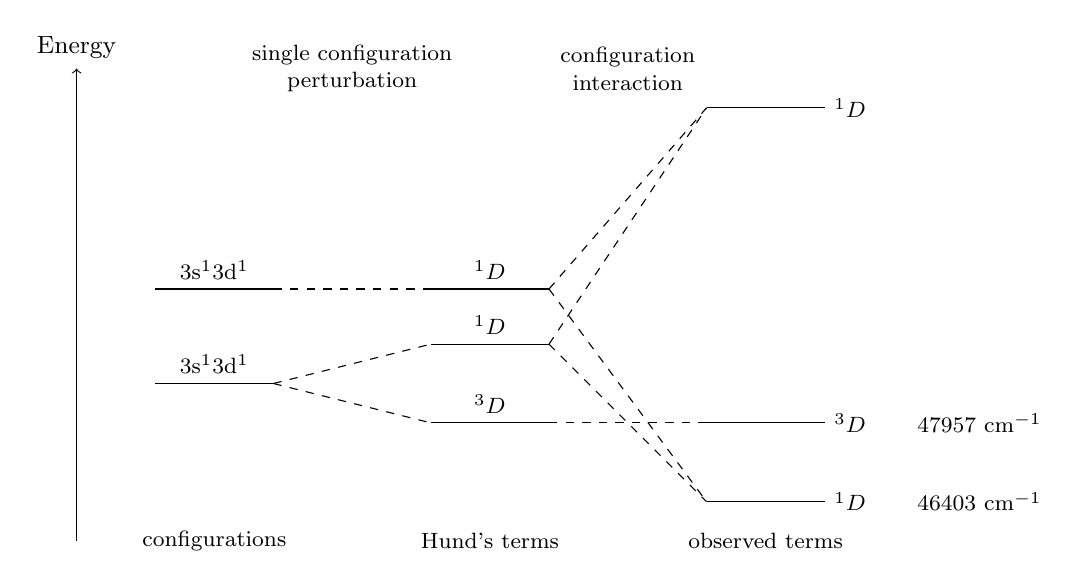
\begin{tikzpicture}
            \draw[->] (0,-0.5)--(0,5.5)node[above]{\small Energy};
            \draw (1,1.5)--node[above]{\footnotesize \(\mathrm{3s^1 3d^1}\)}(2.5,1.5);
            \draw (1,2.7)--node[above]{\footnotesize \(\mathrm{3s^1 3d^1}\)}(2.5,2.7);
            \draw (4.5,1)--node[above]{\footnotesize \(^3D\)}(6,1);
            \draw (4.5,2)--node[above]{\footnotesize \(^1D\)}(6,2);
            \draw (4.5,2.7)--node[above]{\footnotesize \(^1D\)}(6,2.7);
            \draw (8,1)--(9.5,1)node[right]{\footnotesize \(^3D\)}node[right=3em]{\footnotesize\(47957\unit{cm}^{-1}\)};
            \draw (8,0)--(9.5,0)node[right]{\footnotesize \(^1D\)}node[right=3em]{\footnotesize\(46403\unit{cm}^{-1}\)};
            \draw (8,5)--(9.5,5)node[right]{\footnotesize \(^1D\)};
            \draw[dashed] (2.5,1.5)--(4.5,1);
            \draw[dashed] (2.5,1.5)--(4.5,2);
            \draw[dashed] (2.5,2.7)--(4.5,2.7);
            \draw[dashed] (6,1)--(8,1);
            \draw[dashed] (6,2)--(8,0);
            \draw[dashed] (6,2)--(8,5);
            \draw[dashed] (6,2.7)--(8,0);
            \draw[dashed] (6,2.7)--(8,5);
            \node at (1.75,-0.5) {\footnotesize configurations};
            \node at (5.25,-0.5) {\footnotesize Hund's terms};
            \node at (8.75,-0.5) {\footnotesize observed terms};
            \node at (3.5,5.5) [align=center] {\footnotesize single configuration \\[-2pt]\footnotesize perturbation};
            \node at (7,5.5) [align=center] {\footnotesize configuration \\[-2pt]\footnotesize interaction};
        \end{tikzpicture}
        \caption{The ordering of the excited \(\mathrm{Mg}\) violates the Hund's rules due to configuration interaction.}
    \end{figure}

    \subsubsection{\texorpdfstring{\(jj\)}{jj} Coupling}
    At the start of this section we said `as long as the splitting from spin-orbit coupling is small compared to the energy difference between terms\dots'. This regime is called `\textit{\(LS\) coupling}' or `\textit{Russell--Saunders coupling}'. The assumption is that \(L\) and \(S\) are reasonably well-defined and the spin-orbit coupling is a small perturbation. If we had included the nuclear charge in (\ref{spin_orbit_coupling}), we would have
    \begin{equation}
        E_{\text{SO},n\ell m;j}^{(1)}=\frac{Z^4}{4c^2}\frac{j(j+1)-\ell(\ell+1)-\frac{3}{4}}{n^3\ell(\ell+\frac{1}{2})(\ell+1)}\,.
    \end{equation}
    The factor \(Z^4\) shows that the magnitude of the spin-orbit coupling increases rapidly with \(Z\), and when we arrive at around Lanthanoids, the electron-electron repulsions and spin-orbit coupling are about the same magnitude, making the idea of treating spin-orbit coupling as a small perturbation no longer appropriate. As we further increase \(Z\), the spin-orbit coupling would be so large that the Coulombic splitting between terms to be small compared to the spin-orbit splitting between levels. By then, we should use a different scheme, called \(jj\) coupling. There is no hard cutoff between \(LS\) coupling and \(jj\) coupling, as in between both effects are similar in magnitude. Beyond about gold we are safely in the \(jj\) coupling regime.

    To apply \(jj\) coupling, first we generate an individual \(j\) for each electron, using the Clebsch-Gordan series to couple the \(l\) and \(s\) of each electron. Then the individual \(j\) are then coupled using the Clebsch-Gordan series to generate the overall \(J\) possibilities.

    \begin{ex}
        Consider the ground state configuration of \(\mathrm{Pb}\), \(\mathrm{6p^2}\) as an example. As with Russell--Saunders coupling, all full shells have zero angular momentum so can be ignored. Each individual electron has \(l=1\) and \(s=\frac{1}{2}\), so for each electron the possibilities for \(j\) are \(\frac{1}{2}\) and \(\frac{3}{2}\). Then we have several ways of combining to get \(J\) values. The Clebsch--Gordan series suggests that for \((\frac{1}{2},\frac{1}{2})\) then \(J=0,1\); for \((\frac{3}{2},\frac{1}{2})\) then \(J=1,2\); and for \((\frac{3}{2},\frac{3}{2})\) then \(J=0,1,2,3\). Evaluating the degeneracies of each of these levels \((2J+1)\) and summing gives 30 states, and yet we know that there should be 15 states: 6 ways to place the first electron, 5 ways to place the second, and the order doesn't matter. This is because we have omitted the Pauli principle, which is relevant because both electrons are in the same shell.

        \begin{figure}
            \centering
            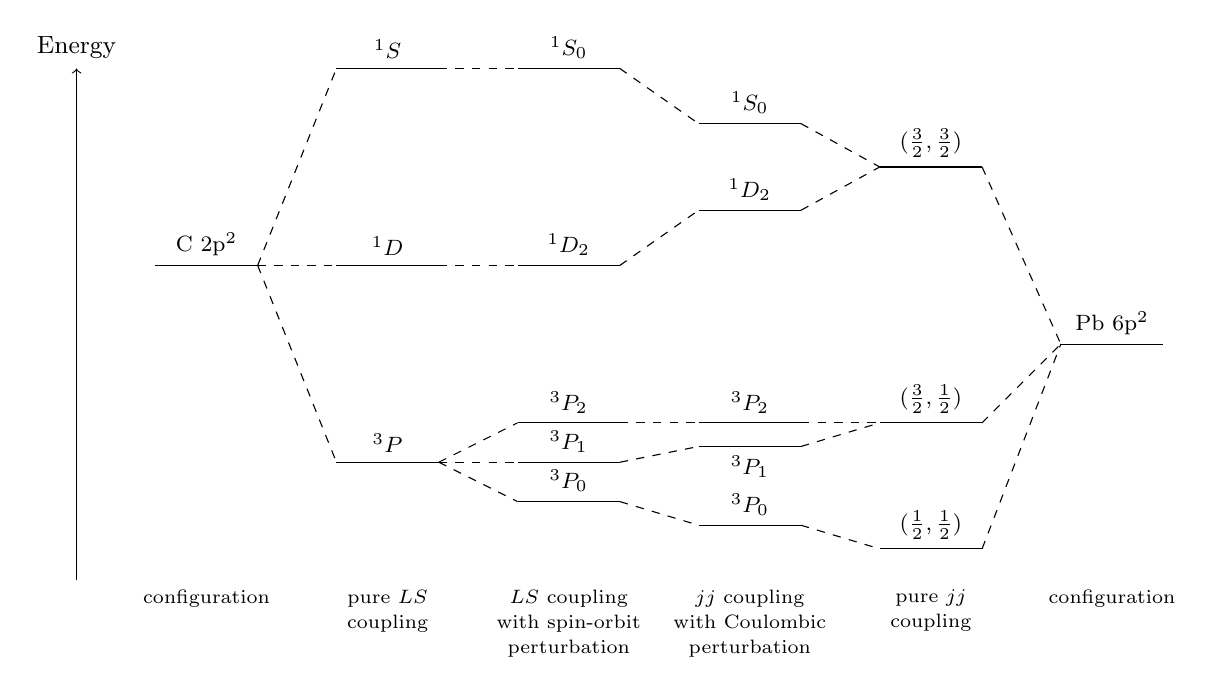
\begin{tikzpicture}
                \draw[->] (0,-0.5)--(0,6)node[above]{\small Energy};
                \draw (1,3.5)--node[above]{\footnotesize \(\mathrm{C}\) \(\mathrm{2p^2}\)}(2.3,3.5)node(a1){};
                \draw (3.3,1)node(b1){}--node[above]{\footnotesize \(^3 P\)}(4.6,1)node(c1){};
                \draw (3.3,3.5)node(b2){}--node[above]{\footnotesize \(^1 D\)}(4.6,3.5)node(c2){};
                \draw (3.3,6)node(b3){}--node[above]{\footnotesize \(^1 S\)}(4.6,6)node(c3){};
                \draw (5.6,0.5)node(d1){}--node[above]{\footnotesize \(^3 P_0\)}(6.9,0.5)node(e1){};
                \draw (5.6,1)node(d2){}--node[above]{\footnotesize \(^3 P_1\)}(6.9,1)node(e2){};
                \draw (5.6,1.5)node(d3){}--node[above]{\footnotesize \(^3 P_2\)}(6.9,1.5)node(e3){};
                \draw (5.6,3.5)node(d4){}--node[above]{\footnotesize \(^1 D_2\)}(6.9,3.5)node(e4){};
                \draw (5.6,6)node(d5){}--node[above]{\footnotesize \(^1 S_0\)}(6.9,6)node(e5){};
                \draw (7.9,0.2)node(f1){}--node[above]{\footnotesize \(^3 P_0\)}(9.2,0.2)node(g1){};
                \draw (7.9,1.2)node(f2){}--node[below]{\footnotesize \(^3 P_1\)}(9.2,1.2)node(g2){};
                \draw (7.9,1.5)node(f3){}--node[above]{\footnotesize \(^3 P_2\)}(9.2,1.5)node(g3){};
                \draw (7.9,4.2)node(f4){}--node[above]{\footnotesize \(^1 D_2\)}(9.2,4.2)node(g4){};
                \draw (7.9,5.3)node(f5){}--node[above]{\footnotesize \(^1 S_0\)}(9.2,5.3)node(g5){};
                \draw (10.2,-0.1)node(h1){}--node[above]{\footnotesize \((\frac{1}{2},\frac{1}{2})\)}(11.5,-0.1)node(i1){};
                \draw (10.2,1.5)node(h2){}--node[above]{\footnotesize \((\frac{3}{2},\frac{1}{2})\)}(11.5,1.5)node(i2){};
                \draw (10.2,4.75)node(h3){}--node[above]{\footnotesize \((\frac{3}{2},\frac{3}{2})\)}(11.5,4.75)node(i3){};
                \draw (12.5,2.5)node(j1){}--node[above]{\footnotesize \(\mathrm{Pb}\) \(\mathrm{6p^2}\)}(13.8,2.5);
                \draw[dashed] (a1.center)--(b1.center);
                \draw[dashed] (a1.center)--(b2.center);
                \draw[dashed] (a1.center)--(b3.center);
                \draw[dashed] (c1.center)--(d1.center);
                \draw[dashed] (c1.center)--(d2.center);
                \draw[dashed] (c1.center)--(d3.center);
                \draw[dashed] (c2.center)--(d4.center);
                \draw[dashed] (c3.center)--(d5.center);
                \draw[dashed] (e1.center)--(f1.center);
                \draw[dashed] (e2.center)--(f2.center);
                \draw[dashed] (e3.center)--(f3.center);
                \draw[dashed] (e4.center)--(f4.center);
                \draw[dashed] (e5.center)--(f5.center);
                \draw[dashed] (g1.center)--(h1.center);
                \draw[dashed] (g2.center)--(h2.center);
                \draw[dashed] (g3.center)--(h2.center);
                \draw[dashed] (g4.center)--(h3.center);
                \draw[dashed] (g5.center)--(h3.center);
                \draw[dashed] (i1.center)--(j1.center);
                \draw[dashed] (i2.center)--(j1.center);
                \draw[dashed] (i3.center)--(j1.center);
                \node at (1.65,-0.5)[below,align=center]{\scriptsize configuration};
                \node at (3.95,-0.5)[below,align=center]{\scriptsize pure \(LS\) \\[-3pt] \scriptsize coupling};
                \node at (6.25,-0.5)[below,align=center]{\scriptsize \(LS\) coupling \\[-3pt] \scriptsize with spin-orbit \\[-3pt] \scriptsize perturbation};
                \node at (8.55,-0.5)[below,align=center]{\scriptsize \(jj\) coupling \\[-3pt] \scriptsize with Coulombic \\[-3pt] \scriptsize perturbation};
                \node at (10.85,-0.5)[below,align=center]{\scriptsize pure \(jj\) \\[-3pt] \scriptsize coupling};
                \node at (13.15,-0.5)[below,align=center]{\scriptsize configuration};
            \end{tikzpicture}
            \caption{A qualitative correlation diagram showing the levels in the \(n\mathrm{p^2}\) ground state configurations of C and Pb.}
            \label{Fig:jj_LS_correlation_diagram}
        \end{figure}

        The statement of the Pauli principle in \(jj\) coupling is that electrons in the same shell with the same \(j\) values must have different \(m_j\) values. As with Russell--Saunders coupling, we can list all the possible combinations of \(m_j\) values, generate the list of \(M_J\) values by addition, and then infer the \(J\) levels that give rise to them. Doing so removes the \(J=1\) level from the \((\frac{1}{2},\frac{1}{2})\) set leaving only \(J=0\). It also removes the \(J=3\) and \(J=1\) levels from the \((\frac{3}{2},\frac{3}{2})\) set, leaving the \(J=0\) and \(J=2\) levels. This has no effect on the \((\frac{3}{2},\frac{1}{2})\) levels as the electrons have different values of \(j\). Overall then, we have \(J=0,0,1,2,2\), for the expected total of 15 states.

        Hund's third rule still applies and we can suggest that sets with smaller \(j\) values will be lower in energy. In the absence of Coulombic effects, the different \(J\) values from the same \((j_1,j_2)\) set would have the same energies, but treating the Coulombic effect as a small perturbation, the levels will split. Quite which way is not easy to see, as we need to apply Hund's first and second rules but we have not worked out \(S\) and \(L\). We make the observation that there must be a continuous and smooth change from the carbon levels to the lead levels as \(Z\) increases, with \(J\) staying unchanged, so we can correlate the levels between the two situations. States with the same \(J\) are also subject to an avoided-crossing rule, so we can unambiguously decide which level ends up where. The correlation diagram is shown in \cref{Fig:jj_LS_correlation_diagram}. The diagram implies that even when we are in the \(jj\) coupling regime, levels can be labelled with their Russell--Saunders term symbols. Although on the \(jj\) side, both \(J=2\) levels, for example, will have a significant contribution from both \(^3P\) and \(^1D\).
    \end{ex}

    \newpage
    \part*{Appendices}
    \addcontentsline{toc}{part}{\protect\numberline{}Appendices}
    \appendix
    
    \section{Convergence of Perturbation Series}\label{Appendix:Converge}
    We began our study of perturbation theory by assuming that the states and energy eigenvalues of the full Hamiltonian depend analytically on a dimensionless parameter \(\lambda\) controlling the perturbation. Even when the individual coefficients of powers of \(\lambda\) are finite, this is often not the case because the infinite perturbative series itself may fail to converge, or may converge only for some range of \(\lambda\). The issue is that the coefficients of \(\lambda\) may grow too rapidly. Heuristically, the condition for convergence is thus that the typical energy splitting \(\mel{m}{H^{(1)}}{n}\) induced by the perturbation should be much smaller than the initial energy difference \(E_m-E_n\). However, a detailed criterion is often hard to come by since the higher terms in the perturbation expansion involve complicated sums (or integrals) over many different intermediate states.

    To illustrate this in a simple context, let's consider in turn the following three perturbations of a 1D harmonic oscillator potential
    \begin{equation}
        \hat{H}=\frac{\hat{p}^2}{2m}+\frac{1}{2}m\omega^2x^2+\begin{cases}
            -\lambda m\omega^2 x_0x\\
            +\frac{1}{2}\lambda m\omega^2x^2\\
            +\lambda\epsilon x^4\,,
        \end{cases}
    \end{equation}
    where \(x_0\) and \(\epsilon\) are constants. Of course, the first two can be solved exactly --- we'd never really use perturbation theory to study them.

    In the first case, we have
    \begin{equation}
        \hat{H}=\frac{\hat{p}^2}{2m}+\frac{1}{2}m\omega^2(x-\lambda x_0)^2-\frac{\lambda^2}{2}m\omega^2x_0^2\,,
    \end{equation}
    from which we easily see that the exact energies are
    \begin{equation}
        E_n(\lambda)=\left(n+\frac{1}{2}\right)\hbar\omega-\frac{\lambda^2}{2}m\omega^2 x_0^2
    \end{equation}
    with corresponding position space wavefunction \(\braket{x}{n_\lambda}=\braket{x-\lambda x_0}{n}\) just a translation of the usual harmonic oscillator wavefunction \(\braket{x}{n}\). If we instead tackled this problem using perturbation theory, we'd find
    \begin{align}
        E_n(\lambda)&=E_n-\lambda m\omega^2 x_0\expval{x}{n}+\lambda^2 m^2 \omega^4 x_0^2 \sum_{k\ne n}\frac{\abs{\mel{k}{x}{n}}^2}{(n-k)\hbar\omega}+O(\lambda^3)\notag\\
        &=\left(n+\frac{1}{2}\right)\hbar\omega-\frac{\lambda^2}{2}m\omega^2 x_0^2 +O(\lambda^3)\,.
    \end{align}
    To obtain this result, we note that the first-order term vanishes (e.g. by symmetry), while since \(x\) is a linear combination of creation and annihilation operators \(\hat{a}^\dagger\) and \(\hat{a}\), only the \(k=n+1\) and \(k=n-1\) terms can contribute to the sum in the second-order term. Going further, we'd find that there are no higher corrections in \(\lambda\) --- the \(O(\lambda^3)\) terms are in fact zero --- though this is not easy to see directly. Thus, in this case, the perturbative result converges to the exact result, and the radius of convergence is infinite. This reflects the fact that the perturbation \(-\lambda m\omega^2 x_0x\) didn't really change the character of the original Hamiltonian. No matter how large \(\lambda\) is, for large enough \(x\) the perturbation remains negligible.

    Turning to the second case, it's again immediate that the exact energy levels are
    \begin{equation}
        E_n(\lambda)=\left(n+\frac{1}{2}\right)\hbar\omega(\lambda)\,,
    \end{equation}
    where \(\omega(\lambda)=\omega\sqrt{1+\lambda}\) is the modified frequency. Viewing as a complex function, it has a branch cut starting at \(\lambda=-1\), so the energy is only analytic in the disc \(\abs{\lambda}<1\). Again using perturbation theory, we find
    \begin{align}
        E_n(\lambda)&=E_n+\frac{\lambda}{2}m\omega^2\expval{x^2}{n}+\frac{\lambda^2}{4}m^2\omega^4\sum_{k\ne n}\frac{\abs{\mel{k}{x^2}{n}}^2}{(n-k)\hbar\omega}+O(\lambda^3)\notag\\
        &=\left(n+\frac{1}{2}\right)\hbar\omega\left(1+\frac{\lambda}{2}-\frac{\lambda^2}{8}+O(\lambda^3)\right)\,,
    \end{align}
    agreeing to this order with the Taylor expansion of the exact answer. Continuing further, we'd find that this Taylor series does indeed converge provided \(\abs{\lambda}<1\), and that it then converges to the exact answer. The physical reason why the perturbation series diverges when \(\abs{\lambda}\ge 1\) is simply that if \(\lambda=-1\), the `perturbation' has completely cancelled the original harmonic oscillator potential, so we are no longer studying a system that can be treated as a harmonic oscillator in the first instance. Once \(\lambda<-1\) the harmonic oscillator potential is turned upside down, and we do not expect our system to possess any stable bound states.

    Finally, consider the case
    \begin{equation}
        \hat{H}=\hat{H}^{(0)}+\lambda\epsilon x^4\,.
    \end{equation}
    I do not know whether this model has been solved exactly, but it can be treated perturbatively. After a fair amount of non-trivial calculation\footnote{You can find the details in Bender, C. and Wu, T.T., \textit{Anharmonic Oscillator II: A Study of Perturbation Theory in Large Order}, Phys. Rev. D7, 1620-1636 (1973)} one obtains the series
    \begin{equation}\label{quartic_perturbation}
        E_0(\lambda)=\frac{1}{2}\hbar\omega+\sum_{n=1}^{\infty}(\lambda\epsilon)^n a_n
    \end{equation}
    for the ground state energy including the quartic interaction, where the coefficients behave as
    \begin{equation}
        a_n=\frac{(-1)^{n+1}\sqrt{6}}{\pi^{3/2}}3^n\Gamma\left(n+\frac{1}{2}\right)\left(1-\frac{95}{72}\frac{1}{n}+O(n^{-2})\right)\,.
    \end{equation}
    On account of the \(\Gamma\)-function, these grow factorially with \(n\), so the series (\ref{quartic_perturbation}) has radius of convergence \(\lambda=0\). Once again, this is easy to see from the form of the perturbed Hamiltonian: even though we may only care about \(\lambda>0\), our assumption that the perturbation expansion is analytic in \(\lambda\) at \(\lambda=0\) means that, if it converges, it will do so for a disc \(\lambda\in D\subset\CC\). For any \(\lambda\in\RR_{<0}\), the Hamiltonian of the quartic oscillator is unbounded below, so there cannot be any stable bound states that are analytic in \(\lambda\) at \(\lambda=0\).

    Let me comment that even when perturbative series do not converge, they may still provide very useful information as an asymptotic series. Briefly, we say a series \(S_N(\lambda)=\sum_{n=0}^{N}a_n\lambda^n\) is \textit{asymptotic} to an exact function \(S(\lambda)\) as \(\lambda\to 0^+\) (written \(S_N(\lambda)\sim S(\lambda)\) as \(\lambda\to 0^+\)) if
    \begin{equation}
        \lim_{\lambda\to 0^+}\frac{1}{\lambda^N}\abs{S(\lambda)-\sum_{n=0}^{N}a_n\lambda^n}=0\,.
    \end{equation}
    In other words, if we just include a fixed number \(N\) of terms in our series, then for small enough \(\lambda\ge 0\) these first \(N\) terms differ from the exact answer by less than \(\epsilon\lambda^N\) for any \(\epsilon>0\) (so the difference is \(o(\lambda^N)\)). However, if we instead try to fix \(\lambda\) and improve our accuracy by including more and more terms in the series, then an asymptotic series will eventually diverge. Most of the perturbative series one meets in the quantum world (including most Feynman diagram expansions in the fancy quantum field theory) are only asymptotic series. Just as in our toy examples above, the radius of convergence of such series is often associated with interesting physics.

    \section{Wigner's \texorpdfstring{\(2n+1\)}{2n+1} Theorem}\label{Appendix:Wigner}
    Let's first reformulate our problem a little bit. We know that the energy of a normalised state \(\psi\) is given by the expectation value of the Hamiltonian \(E=\expval{\hat{H}}{\psi}\). This allows us to consider the energy as a functional
    \begin{equation}
        E[\psi,\lambda]=\expval{\hat{H}}{\psi}=\expval{\hat{H}^{(0)}+\lambda\hat{H}^{(1)}}{\psi}\,.
    \end{equation}
    For example, in the unperturbed situation where \(\lambda=0\), the ground state energy is given by the minimum of the energy functional
    \begin{equation}
        E_{\text{min}}=E[\psi_0^{(0)},0]\,,
    \end{equation}
    where \(\psi_0^{(0)}\) is the ground state wavefunction of the unperturbed Hamiltonian. By the Rayleigh--Ritz variational principle, all eigenstates of the Hamiltonian \(\hat{H}\) are the stationary values of the energy functional. Therefore, to find the \(k^{\text{th}}\) eigenstate of \(\hat{H}\) for any \(\lambda\), we can write \(\psi_k=\psi_k^{(0)}+\Delta\psi_k\), and find the \(\Delta\psi_k\) which satisfies
    \begin{equation}
        \pdv{E[\psi_k^{(0)}+\Delta\psi_k,\lambda]}{(\Delta\psi_k)}=0\,,
    \end{equation}
    and then the eigenvalue (energy) will be given by \(E_k(\lambda)=E[\psi_k^{(0)}+\Delta\psi_k,\lambda]\). From now on, we will drop the subscript \(k\) to refer to any eigenstate. If the perturbation \(\lambda\) is small, then we can expand the eigenstates and the eigenvalues as a Taylor series (as what we did in the normal perturbation theory)
    \begin{align}
        \Delta\psi&=\sum_{n=1}^{\infty}\frac{1}{n!}\pdv[n]{\psi}{\lambda}\bigg|_{\lambda=0}\equiv\sum_{n=1}^{\infty}\psi^{(n)}\lambda^n \label{delta_psi_expansion}\\
        E&=\sum_{n=0}^{\infty}\frac{1}{n!}\pdv[n]{E}{\lambda}\bigg|_{\lambda=0}\equiv \sum_{n=0}^{\infty}E^{(n)}\lambda^n\,.
    \end{align}
    Then what we want to claim is that we only need to know \(\psi^{(i)}\) for \(i=1,\dots,n\) to calculate \(E^{(2n+1)}\). Before proving this, we need some preparations.

    First, let's expand the functional \(E[\psi^{(0)}+\Delta\psi,\lambda]\) in both \(\Delta\psi\) and \(\lambda\). We get the double series
    \begin{equation}\label{energy_double_expansion}
        E=E[\psi^{(0)}+\Delta\psi,\lambda]=\sum_{k=0}^{\infty}\sum_{p=0}^{\infty}\frac{1}{k!}\frac{1}{p!}\frac{\delta^{k+p}E[\psi^{(0)}+\Delta\psi,\lambda]}{\delta(\Delta\psi)^k\delta\lambda^p}\bigg|_{\Delta\psi=0,\lambda=0}(\Delta\psi)^k\lambda^p\,.
    \end{equation}
    Then for \(\psi=\psi^{(0)}+\Delta\psi\) to be an eigenstate, we need to set \(\partial E[\psi^{(0)}+\Delta\psi,\lambda]/\partial(\Delta\psi)\) to zero, which is evaluated as
    \begin{equation}
        \pdv{E[\psi^{(0)}+\Delta\psi,\lambda]}{(\Delta\psi)}=\sum_{k=1}^{\infty}\sum_{p=0}^{\infty}\frac{1}{(k-1)!}\frac{1}{p!}\frac{\delta^{k+p}E[\psi^{(0)}+\Delta\psi,\lambda]}{\delta(\Delta\psi)^k\delta\lambda^p}\bigg|_{\Delta\psi=0,\lambda=0}(\Delta\psi)^{k-1}\lambda^p\,.
    \end{equation}
    For simplicity, we denote
    \begin{equation}
        f^{(p)}\coloneqq\sum_{k=1}^{\infty}\frac{1}{(k-1)!}\frac{1}{p!}\frac{\delta^{k+p}E[\psi^{(0)}+\Delta\psi,\lambda]}{\delta(\Delta\psi)^k\delta\lambda^p}\bigg|_{\Delta\psi=0,\lambda=0}(\Delta\psi)^{k-1}\,,
    \end{equation}
    and so the above expression reduces to
    \begin{equation}
        \pdv{E[\psi^{(0)}+\Delta\psi,\lambda]}{(\Delta\psi)}=\sum_{p=0}^{\infty}f^{(p)}\lambda^p=0\,.
    \end{equation}
    For this to hold for all \(\lambda\), we must have \(f^{(p)}=0\) for all \(p\).

    Next, let's have a closer look at our energy expansion
    \begin{equation}
        E=\sum_{n=0}^{\infty}E^{(n)}\lambda^n=\sum_{k=0}^{\infty}\sum_{p=0}^{\infty}c_{kp}(\Delta\psi)^k\lambda^p
    \end{equation}
    for some complicated coefficients \(c_{kp}\) given in (\ref{energy_double_expansion}). Here we can use the series expansion (\ref{delta_psi_expansion}) for \(\Delta\psi\)
    \begin{equation}
        \Delta\psi=\sum_{n=1}^{\infty}\psi^{(n)}\lambda^n
    \end{equation}
    so that
    \begin{equation}
        E=\sum_{n=0}^{\infty}E^{(n)}\lambda^n=\sum_{k=0}^{\infty}\sum_{p=0}^{\infty}c_{kp}\left(\sum_{n=1}^{\infty}\psi^{(n)}\lambda^n\right)^k\lambda^p
    \end{equation}
    Now consider the terms contributing to \(E^{(2n+1)}\lambda^{2n+1}\) in the above expansion. We claim that the terms must be linear in \(\psi^{(G)}\lambda^G\) for all \(G>n\). This is because if there is any quadratic (or above) term, then
    \begin{equation}
        E^{(2n+1)}\lambda^{2n+1}\sim[\psi^{(G)}\lambda^G]^2\sum_{p=0}^{\infty}\lambda^p={\psi^{(G)}}^2\underbrace{\lambda^{2G}\sum_{p=0}^{\infty}\lambda^p}_{\lambda^{2n+2}\text{ or higher}}\,.
    \end{equation}
    The power of \(\lambda\) is at least \(2n+2\), so it cannot contribute to \(E^{(2n+1)}\lambda^{2n+1}\). Then, we can write \((\Delta\psi)^k\) in the following way:
    \begin{align}
        (\Delta\psi)^k&=\left[\sum_{n=1}^{k}\psi^{(n)}\lambda^n\right]^k=[\psi^{(1)}\lambda+\psi^{(2)}\lambda^2+\dots+\psi^{(G)}\lambda^G+\dots][\psi^{(1)}\lambda+\psi^{(2)}\lambda^2+\dots]\dots \notag\\
        &=\sum_{a=k}^{nk}P^{(a)}(\psi^{(1)},\psi^{(2)},\dots,\psi^{(n)})\lambda^a + k\psi^{(G)}\lambda^{G}(\Delta\psi)^{k-1}+[\text{higher order terms.}]
    \end{align}
    The first term is a polynomial \(P\) of \(\psi^{(1)}\) up until \(\psi^{(n)}\), coming from picking a lower-than-\(\psi^{(n)}\lambda^n\) term from each of the square brackets in the first line. The second term pulls out a single \(\psi^{(G)}\lambda^G\) from one of the brackets, and there should be \(k\) terms like that. Technically this term is at least linear in \(\psi^{(G)}\lambda^G\), since \((\Delta\psi)^{k-1}\) will certainly contain \(\psi^{(G)}\lambda^G\) in each factor of \(\Delta\psi\), but this expansion is good enough to prove what we want. Finally, we are left with terms in which \(\psi^{(G)}\lambda^G\) appears twice or more often, and we are not interested in those.

    Finally, to prove \(2n+1\) theorem, we only need to plug this horrible-looking expansion of \((\Delta\psi)^k\) into our Taylor expansion of \(E\) (\ref{energy_double_expansion}).
    \begin{align}
        E=\sum_{k=0}^{\infty}\sum_{p=0}^{\infty}\frac{1}{k!}\frac{1}{p!}&\frac{\delta^{k+p}E[\psi^{(0)}+\Delta\psi,\lambda]}{\delta(\Delta\psi)^k\delta\lambda^p}\bigg|_{\Delta\psi=0,\lambda=0}\notag\\
        &\left[\sum_{a=k}^{nk}P^{(a)}(\psi^{(1)}\dots,\psi^{(n)})\lambda^a + k\psi^{(G)}\lambda^{G}(\Delta\psi)^{k-1}+[\text{H.O.T.}]\right]\lambda^p\,,
    \end{align}
    where \(G>n\). Now consider terms contributing to \(E^{(2n+1)}\lambda^{2n+1}\). They are
    \begin{align}
        E^{(2n+1)}\lambda^{2n+1}&=\sum_{k=0}^{\infty}\sum_{p=0}^{\infty}\frac{1}{k!p!}\frac{\delta^{k+p}E[\psi^{(0)}+\Delta\psi,\lambda]}{\delta(\Delta\psi)^k\delta\lambda^p}\bigg|_{\Delta\psi=0,\lambda=0}\sum_{a=k}^{nk}P^{(a)}(\psi^{(1)}\dots,\psi^{(n)})\lambda^{a+p}\bigg|_{a+p=2n+1}\notag\\
        &\quad+\sum_{p=0}^{\infty}\underbrace{\sum_{k=1}^{\infty}\frac{1}{(k-1)!p!}\frac{\delta^{k+p}E[\psi^{(0)}+\Delta\psi,\lambda]}{\delta(\Delta\psi)^k\delta\lambda^p}\bigg|_{\Delta\psi=0,\lambda=0}(\Delta\psi)^{k-1}}_{f^{(p)}}\psi^{(G)}\lambda^{G+p}\bigg|_{p+G=2n+1}\,.
    \end{align}
    Since \(f^{(p)}=0\), the second term vanishes, and we are only left with
    \begin{equation}
        E^{(2n+1)}\lambda^{2n+1}=\sum_{k=0}^{\infty}\sum_{p=0}^{\infty}\frac{1}{k!p!}\frac{\delta^{k+p}E[\psi^{(0)}+\Delta\psi,\lambda]}{\delta(\Delta\psi)^k\delta\lambda^p}\bigg|_{\Delta\psi=0,\lambda=0}\sum_{a=k}^{nk}P^{(a)}(\psi^{(1)}\dots,\psi^{(n)})\lambda^{a+p}\bigg|_{a+p=2n+1}\,.
    \end{equation}
    Only \(\psi^{(1)},\dots,\psi^{(n)}\) are present in this expression. This completes the proof.\qed

    \section{More on the Polarisability of Hydrogen}\label{Chap:Hydrogen_Polarisability}
    \subsection{Rayleigh--Schr\"{o}dinger Sum Involving Continuum States}
    The Rayleigh--Schr\"{o}dinger sum of the polarisability of hydrogen atom is given by
    \begin{equation}
        \alpha=2\sum_{k\ne 0}\frac{\abs{\mel{0}{z}{k}}^2}{E_k^{(0)}-E_0^{(0)}}\,.
    \end{equation}
    Here \(\ket{k}\) should include both the bound states and the continuum states. Let's first consider the bound states, which can be labelled by \(\ket{n,\ell,m_\ell}\). We can separate this integral into radial and angular parts,
    \begin{equation}
        \mel{0}{z}{n,\ell,m_\ell}=\mel{Y_{00}}{\cos\theta}{Y_{\ell m_\ell}}\mel{R_{1\mathrm{s}}}{r}{R_{n\ell}}\,,
    \end{equation}
    where \(Y_{\ell m_\ell}\) are the spherical harmonics. Since
    \begin{equation}
        Y_{00}=\frac{1}{2}\sqrt{\frac{1}{\pi}}\,,\quad Y_{10}=\frac{1}{2}\sqrt{\frac{3}{\pi}}\cos\theta\,,
    \end{equation}
    we can evaluate the angular part to
    \begin{align}
        \mel{Y_{00}}{\cos\theta}{Y_{\ell m_\ell}}&=\frac{1}{\sqrt{3}}\braket{Y_{10}}{Y_{\ell m_\ell}}=\frac{1}{\sqrt{3}}\delta_{1\ell}\delta_{0 m_\ell}
    \end{align}
    by the orthonormality of spherical harmonics. Thus we need the \(\mathrm{p}_z\) orbitals only. We can also put in the energy expressions \(E_0^{(0)}=-\frac{1}{2}\), \(E_n^{(0)}=-\frac{1}{2n^2}\), giving
    \begin{equation}
        \alpha_{\text{bound}}=\frac{4}{3}\sum_{n=2}^{\infty}\frac{\abs{\mel{R_{1\mathrm{s}}}{r}{R_{n\mathrm{p}}}}^2}{1-n^{-2}}\,.
    \end{equation}
    To proceed, we need the radial wavefunctions. In atomic units, it is given by
    \begin{equation}
        R_{n\ell}(r)=\frac{2}{n^2}\sqrt{\frac{(n-\ell-1)!}{2n (n+\ell)!}}\ee^{-\frac{r}{n}}\left(\frac{2r}{n}\right)^{\ell}L_{n-\ell-1}^{(2\ell+1)}\left(\frac{2r}{n}\right)\,,
    \end{equation}
    where \(L_m^{(\alpha)}\) is the generalised (associated) Laguerre polynomial of degree \(m\).\footnote{There are unfortunately different conventions defining the generalised Laguerre functions, so you may see different forms of this in different literatures. Here we define \(L_m^{(\alpha)}\) as the power series solution of the differential equation
    \begin{equation}
        xy''+(\alpha+1-x)y'+my=0\,,
    \end{equation}
    where \(m\) is a non-negative integer (necessary for the solution to be a finite-term power series), and \(\alpha\) can be any real number. It is linked to the more consistently defined confluent hypergeometric function in a way that we will mention later.} We will only need the \(1\mathrm{s}\) radial wavefunction
    \begin{equation}
        R_{1\mathrm{s}}(r)=2e^{-r}
    \end{equation}
    and the \(n\mathrm{p}\) wavefunction
    \begin{equation}
        R_{n\mathrm{p}}(r)=4\sqrt{\frac{1}{n^7(n^2-1)}}re^{-r/n}L_{n-2}^{(3)}\left(\frac{2r}{n}\right)\,.
    \end{equation}
    There is no good reason to assume that we can treat this sum analytically, so we can do this numerically on a computer.

    \begin{table}
        \centering
        \begin{tabular}{cc}
            \toprule
            \(n\) & Contributions summed up to \(n\) \\ \midrule
            2 & 2.959621106 \\
            5 & 3.552510445 \\
            10 & 3.634363556 \\
            20 & 3.655782791 \\
            50 & 3.662031178 \\
            100 & 3.662948342 \\
            200 & 3.663180129 \\
            500 & 3.663245412 \\
            1000 & 3.663254768 \\
            2000 & 3.663257109 \\
            5000 & 3.663257765 \\ \bottomrule
        \end{tabular}
        \caption{Numerical sum of the hydrogen polarisability including contributions up to \(n\mathrm{p}\) orbital.}
    \end{table}

    We see that the sum converges to something close to \(\alpha_{\text{bound}}\approx 3.66326\). As stated in the main text, the sum converges slowly, and to the wrong value. We also need to include the contributions of the unbounded states with energies above \(0\). They correspond to ionised free electrons, and the energy becomes continuous rather than discrete, so they are also known as the continuum states.

    An inspection on the Hamiltonian reveals that these continuum states should have the same angular dependence as the bound states, and the only way to get a positive energy from the expression is if \(n^2<0\), so we would have an imaginary \(n\). These observations suggest that we need to evaluate
    \begin{equation}
        \alpha_{\text{unbound}}=\frac{4}{3}\int_{0}^{\ii\infty}\dd{n}\frac{\abs{\mel{R_{1\mathrm{s}}}{r}{R_{n\mathrm{p}}}}^2}{1-n^{-2}}\,.
    \end{equation}
    This integral is over purely imaginary \(n\), so a first step would be to change the integration variable to a real variable. The energy \(E\) is a good choice, so
    \begin{equation}
        \alpha_{\text{unbound}}=\frac{2}{3}\int_{0}^{\infty}\dd{E}\frac{\abs{\mel{R_{1\mathrm{s}}}{r}{R_{E\mathrm{p}}}}^2}{E+\frac{1}{2}}\,.
    \end{equation}
    However, we would still need to adapt the radial wavefunction for complex \(n\), as the generalised polynomials are only defined for integer degree. Generalised Laguerre polynomials can be written as
    \begin{equation}
        L_n^{(\alpha)}(x)=\frac{\Gamma(\alpha+n+1)}{\Gamma(\alpha+1)\Gamma(n+1)}{_1F_1}(-n,\alpha+1,x)\,,
    \end{equation}
    where \(_1F_1\) is the \textit{confluent hypergeometric function of the first kind}. It is defined for non-integer parameters.\footnote{The confluent hypergeometric function (also known as the Kummer's function) is the solution to the power series solution to the differential equation
    \begin{equation}
        xy''+(b-x)y'-ay=0\,.
    \end{equation}
    We can see that if \(a\) is a non-positive integer, then this reduces to the differential equation defining the generalised Laguerre polynomials.} Therefore, the radial continuum wavefunctions can be written as
    \begin{equation}
        R_{E\ell}(r)=\sqrt{\frac{2k}{\pi}}\ee^{\frac{\pi}{2k}}\frac{\abs{\Gamma\left(\ell+1+\frac{\ii}{k}\right)}}{(2\ell +1)!}(2kr)^{\ell}\ee^{-\ii kr}{_1F_1}\left(\ell+1+\frac{\ii}{k},2\ell+2,2\ii kr\right)\,,
    \end{equation}
    where \(k=\sqrt{2E}\) is the wavenumber. This expression is actually the same form as the bound state expression other than the normalisation factor. The key difference is the \(\ee^{-\ii kr}\) term. For the unbound states, the wavenumber is real, meaning a complex exponential, so oscillations of the wavefunction. For the bound states, the energy is negative so the wavenumber is complex, giving a real exponential that decays with \(r\).

    We are only interested in the \(\ell=1\) case, so the expression simplifies to
    \begin{equation}
        R_{E_p}(r)=\sqrt{\frac{2k}{r}}\ee^{\frac{\pi}{2k}}\abs{\Gamma\left(2+\frac{\ii}{k}\right)}\frac{kr}{3}\ee^{-\ii kr}{_1F_1}\left(2+\frac{\ii}{k},4,2\ii kr\right)\,.
    \end{equation}
    Evaluating this integral numerically gives a continuum contribution \(\alpha_{\text{unbound}}\approx 0.83674\).\footnote{In practice, there are some numerical issues to worry about. The continuum wavefunctions oscillate forever and to not converge to \(0\) as \(r\to\infty\). However, the exponential decay of the 1s wavefunction does ensure a bounded result of \(\mu_E=\mel{R_{1\mathrm{s}}}{r}{R_{E\mathrm{p}}}\).We cannot evaluate \(\mu_E\) at \(E=0\) since the wavefunction is undefined there, but it tends to 0 everywhere as \(E\to 0\) from above. The increasing denominator of the energy also ensures the contribution decreases as the energy increases and the energy integral
    \begin{equation}
        \alpha_{\text{unbound}}=\frac{2}{3}\int_{0}^{\infty}\dd{E}\frac{\mu_E^2}{E+\frac{1}{2}}
    \end{equation}
    does converge. A lower limit of \(r=10^{-7}a_0\) and an upper limit of \(r=100 a_0\) would give sufficient precision, with the greater error coming from a lower bound above \(0\).} Combining all of these together, we get \(\alpha\approx 3.66326+0.83674\approx 4.5\).

    \subsection{Alternative Method Finding the Exact Hydrogen Polarisability}

    There is actually a way finding out the polarisability of hydrogen atom, originally due to A. Dalgarno and J.T. Lewis, not involving solving the first-order wavefunction analytically in the parabolic coordinates, or evaluating the complicated Rayleigh-Schr\"{o}dinger sum numerically.

    Suppose there is an operator \(\hat{X}\) such that \(\hat{H}^{(1)}=[\hat{X},\hat{H}^{(0)}]\), then
    \begin{align}
        \mel{m}{\hat{H}^{(1)}}{n}&=\mel{m}{\hat{X}\hat{H}^{(0)}}{n}-\mel{m}{\hat{H}^{(0)}\hat{X}}{n}\notag \\
        &=(E_n^{(0)}-E_m^{(0)})\mel{m}{\hat{X}}{n}\,.
    \end{align}
    We can then simplify the Rayleigh--Schr\"{o}dinger sum of the second-order energy as
    \begin{align}
        E_n^{(2)}&=-\sum_{m\ne n}\frac{\mel{n}{\hat{H}^{(1)}}{m}(E_n^{(0)}-E_m^{(0)})\mel{m}{\hat{X}}{n}}{E_m^{(0)}-E_n^{(0)}}\notag \\
        &=\sum_{m\ne n}\mel{n}{\hat{H}^{(1)}}{m}\mel{m}{\hat{X}}{n}\notag \\
        &=\mel{n}{\hat{H}^{(1)}\left(\sum_m\ket{m}\bra{m}\right)\hat{X}}{n}-\expval{\hat{H}^{(1)}}{n}\expval{\hat{X}}{n}\notag \\
        &=\expval{\hat{H}^{(1)}\hat{X}}{n}-\expval{\hat{H}^{(1)}}{n}\expval{\hat{X}}{n}\,,\label{second_order_energy_X}
    \end{align}
    where we have cleverly used the resolution of identity to eliminate the sum over all states. Now the task reduces to finding the operator \(\hat{X}\). It turns out that this is not difficult to do. We have
    \begin{equation}
        [\hat{X},\hat{H}^{(0)}]\ket{0}=\hat{H}^{(1)}\ket{0}=\mathcal{E}z\ket{0}\,.
    \end{equation}
    This is just a differential equation that can be solved by separation of variable, and we have
    \begin{equation}
        \hat{X}=-\mathcal{E}\left(\frac{1}{2}r+1\right)z\,.
    \end{equation}
    The expectation values in (\ref{second_order_energy_X}) is easily calculated by exploiting spherical symmetry. The second term vanishes since \(\mel{n}{\hat{H}^{(1)}}{n}=0\), so we have
    \begin{align}
        E_0^{(2)}&=\mathcal{E}\expval{z\hat{X}}{0}\notag \\
        &=-\mathcal{E}^2\expval{\left(\frac{1}{2}r+1\right)z^2}{0}\notag\\
        &=-\frac{1}{3}\mathcal{E}^2\expval{\left(\frac{1}{2}r+1\right)(x^2+y^2+z^2)}{0}\notag\\
        &=-\frac{1}{3}\mathcal{E}^2\left[\frac{1}{2}\expval{r^3}{0}+\expval{r^2}{0}\right]\,.
    \end{align}
    This will give us \(E_0^{(2)}=-\frac{9}{4}\) and so \(\alpha=\frac{9}{2}\) exactly.


    \section{Wavefunctions in the Degenerate Perturbation Theory}\label{Chap:degenerate_PT_first_order_wavefunction}

    Following the main text, we have split the unperturbed wavefunctions into two subsets: \(\left\{\ket{\psi_i^{(0)}}\right\}\) that are non-degenerate with the state of interest, and \(\left\{\ket{\Phi_{nj}^{(0)}}\right\}\) that are degenerate with the state of interest. All of the states in the two sets combined are orthonormal, and we impose the intermediate normalisation such that
    \begin{equation}
        \braket{\Phi_{nj}^{(0)}}{\psi_{nj}^{(1)}}=0\,.
    \end{equation}
    We will split the first-order wavefunction into the contribution from the non-degenerate states labelled ND and the degenerate states labelled D
    \begin{equation}
        \ket{\psi_{nj}^{(1)}}=\ket{\psi_{nj,\text{ND}}^{(1)}}+\ket{\psi_{nj,\text{D}}^{(1)}}=\sum_{k\ne n}c_{k,\text{ND}}\ket{\psi_k^{(0)}}+\sum_{l\ne j}c_{l,\text{D}}\ket{\Phi_{nl}^{(0)}}\,.
    \end{equation}
    The first-order equation for a wavefunction in the degenerate set is
    \begin{equation}
        (\hat{H}^{(0)}-E_n^{(0)})\ket{\psi_{nj}^{(1)}}+(\hat{H}^{(1)}-E_{nj}^{(1)})\ket{\Phi_{nj}^{(0)}}=0\,.
    \end{equation}
    If we contract this with \(\bra{\Phi_{nm}^{(0)}}\) for some \(m\), we get expression of the first-order energy that we find in the main text. If we instead contract with \(\bra{\psi_i^{(0)}}\), we obtain
    \begin{equation}
        c_{i,\text{ND}}=\braket{\psi_i^{(0)}}{\psi_{nj}^{(1)}}=-\frac{\mel{\psi_i^{(0)}}{\hat{H}^{(1)}}{\Phi_{nj}^{(0)}}}{E_i^{(0)}-E_n^{(0)}}\,,
    \end{equation}
    and so the non-degenerate contribution to the first-order wavefunction is
    \begin{equation}
        \ket{\psi_{nj,\text{ND}}^{(1)}}=-\sum_{k\ne n}\frac{H_{kj}^{(1)}}{E_k^{(0)}-E_n^{(0)}}\ket{\psi_k^{(0)}}
    \end{equation}
    as in the normal Rayleigh--Schr\"{o}dinger sum.

    To work out the degenerate coefficients, we need a bit more effort. Consider the second-order equation
    \begin{equation}
        (\hat{H}^{(0)}-E_n^{(0)})\ket{\psi_{nj}^{(2)}}+(\hat{H}^{(1)}-E_{nj}^{(1)})\ket{\psi_{nj}^{(1)}}-E_{nj}^{(2)}\ket{\Phi_{nj}^{(0)}}=0\,.
    \end{equation}
    Contracting with \(\bra{\Phi_{nm}^{(0)}}\) for some \(m\) gives
    \begin{align}
        E_{nj}^{(2)}\delta_{jm}&=\mel{\Phi_{nm}^{(0)}}{\hat{H}^{(1)}-E_{nj}^{(1)}}{\psi_{nj}^{(1)}}\notag\\
        &=\sum_{k\ne n}c_{k,\text{ND}}\mel{\Phi_{nm}^{(0)}}{\hat{H}^{(1)}-E_{nj}^{(1)}}{\psi_k^{(0)}}+\sum_{l\ne j}c_{l,\text{D}}\mel{\Phi_{nm}^{(0)}}{\hat{H}^{(1)}-E_{nj}^{(1)}}{\Phi_{nl}^{(0)}}\notag\\
        &=\sum_{k\ne n}c_{k,\text{ND}}\mel{\Phi_{nm}^{(0)}}{\hat{H}^{(1)}}{\psi_k^{(0)}}+c_{m,\text{D}}(E_{nm}^{(1)}-E_{nj}^{(1)})
    \end{align}
    using the fact that \(\left\{\Phi_{nl}^{(0)}\right\}\) diagonalises \(\hat{H}^{(1)}\) in its span. If we choose \(m=j\), the second term vanishes and we arrive at the second-order energy expression we claimed in the main text
    \begin{equation}
        E_{nj}^{(2)}=\sum_{k\ne n}c_{k,\text{ND}}\mel{\Phi_{nj}^{(0)}}{\hat{H}^{(1)}}{\psi_k^{(0)}}=-\sum_{k\ne n}\frac{\abs{H_{jk}^{(1)}}^2}{E_k^{(0)}-E_n^{(0)}}\,.
    \end{equation}
    If we instead choose \(j\ne m\), the term on the left vanishes and we get
    \begin{equation}
        c_{m,\text{D}}=-\frac{1}{E_{nm}^{(1)}-E_{nj}^{(1)}}\sum_{k\ne n}c_{k,\text{ND}}\mel{\Phi_{nm}^{(0)}}{\hat{H}^{(1)}}{\psi_k^{(0)}}=\frac{1}{E_{nm}^{(1)}-E_{nj}^{(1)}}\sum_{k\ne n}\frac{H_{mk}^{(1)}H_{kj}^{(1)}}{E_k^{(0)}-E_n^{(0)}}\,.
    \end{equation}

    This gives us the total expression of the first-order wavefunction
    \begin{equation}
        \ket{\psi_{nj}^{(1)}}=-\sum_{k\ne n}\frac{H_{kj}^{(1)}}{E_k^{(0)}-E_n^{(0)}}\ket{\psi_k^{(0)}}+\sum_{k\ne n}\sum_{l\ne j}\frac{H_{lk}^{(1)}H_{kj}^{(1)}}{(E_k^{(0)}-E_n^{(0)})(E_{nl}^{(1)}-E_{nj}^{(1)})}\ket{\Phi_{nl}^{(0)}}\,.
    \end{equation}



    \section{The Three Pictures}\label{Chap:Three_Pictures}
    Our formulation of quantum mechanics so far is known as the \textit{Schr\"{o}dinger picture}: a quantum state evolves with time following the Schr\"{o}dinger equation
    \begin{equation}\label{time_dependent_Schrodinger_eqn}
        \ii\hbar\dv{}{t}\ket{\psi}=\hat{H}\ket{\psi}\,,
    \end{equation}
    and observables are associated with operators that (usually) do not change with time, such that the expectation value of a physical quantity \(A\) is given by
    \begin{equation}
        \eval{A}(t)=\expval{\hat{A}}{\psi(t)}\,.
    \end{equation}

    We shall have a bit more careful consideration on the role of time.

    \subsection{State Propagation}
    Any general state can be expanded as a linear combination of the eigenstates of \(\hat{H}\)
    \begin{equation}\label{Schrodinger_expansion}
        \ket{\psi(t)}=\sum_n c_n\ket{n}\,.
    \end{equation}
    We can also expand it in the eigenstates of any other Hermitian operators. Hence, the set of possible outcomes of a measurement and eigenstates of an observable do not change with time. It is the relative weights \(c_n(t)\) that change with time.

    For now, let's assume that the Hamiltonian is time independent. Substituting the expansion (\ref{Schrodinger_expansion}) into the Schr\"{o}dinger equation (\ref{time_dependent_Schrodinger_eqn}), we get
    \begin{align}
        \ii\hbar\sum_n\dv{c_n(t)}{t}\ket{n}&=\sum_n c_n(t)\hat{H}\ket{n}\,,\notag\\
        \ii\hbar\dv{c_n(t)}{t}&=c_n(t)E_n
    \end{align}
    Solving this gives
    \begin{equation}
        c_n(t)=c_n(0)\ee^{-\ii E_nt/\hbar}\,.
    \end{equation}
    Therefore, for a time-independent Hamiltonian, the state evolves as
    \begin{equation}
        \ket{\psi(t)}=\sum_n \ee^{-\ii E_n t/\hbar}c_n(0)\ket{n}\,,
    \end{equation}
    where it is common to denote \(\omega_n\coloneqq E_n/\hbar\). If only one frequency component is present, the energy is certain and the form of the states does not change with time --- it is known as a stationary state.

    The function of an operator is defined as
    \begin{equation}
        f(\hat{X})\ket{\psi_n}=f(x_n)\ket{\psi_n}\,,
    \end{equation}
    where \(\hat{X}\ket{\psi_n}=x_n\ket{\psi_n}\), and its action on a general state is defined by eigenstate expansion, so it has the ket-bra form
    \begin{equation}
        f(\hat{X})=\sum_n f(x_n)\ket{\psi_n}\bra{\psi_n}\,.
    \end{equation}
    Therefore, we can write
    \begin{equation}
        \ket{\psi(t)}=\ee^{-\ii\hat{H}t/\hbar}\ket{\psi(0)}\,.
    \end{equation}
    This is often denoted as the \textit{time shift operator}
    \begin{equation}
        \hat{U}(t,t_0)=\ee^{-\ii\hat{H}(t-t_0)/\hbar}=\sum_n \ee^{-\ii\omega_n(t-t_0)}\ket{n}\bra{n}
    \end{equation}
    so that
    \begin{equation}
        \ket{\psi(t)}=\hat{U}(t,t_0)\ket{\psi(t_0)}\,.
    \end{equation}
    It is easily verified that \(\hat{U}(t-t_0)\) is unitary.

    \subsection{Time-Dependent Hamiltonian}
    Now we allow the Hamiltonian to have time dependence. If we put \(\ket{\psi(t')}=\hat{U}(t',t_0)\ket{\psi(t_0)}\) into the Schr\"{o}dinger equation, we get
    \begin{equation}
        \ii\hbar\dv{}{t'}\hat{U}(t',t_0)=\hat{H}(t')\hat{U}(t',t_0)\,.
    \end{equation}
    We integrate both sides from \(t_0\) to \(t\) and we get
    \begin{equation}
        \hat{U}(t,t_0)=1+\frac{-\ii}{\hbar}\int_{t_0}^{t}\dd{t'}\hat{H}(t')\hat{U}(t',t_0)\,,
    \end{equation}
    where we used \(\hat{U}(t_0,t_0)=1\). This can be solved by iteration, where we substitute the expression itself to \(\hat{U}(t',t_0)\) on the right-hand side repeatedly and get
    \begin{align}\label{propagator_expansion}
        \hat{U}(t,t_0)&=1+\frac{-\ii}{\hbar}\int_{t_0}^{t}\dd{t_1}\hat{H}(t_1)+\left(\frac{-\ii}{\hbar}\right)^2\int_{t_0}^{t}\dd{t_1}\int_{t_0}^{t_1}\dd{t_2}\hat{H}(t_1)\hat{H}(t_2)\notag \\
        &\quad\ +\left(\frac{-\ii}{\hbar}\right)^3\int_{t_0}^{t}\dd{t_1}\int_{t_0}^{t_1}\dd{t_2}\int_{t_0}^{t_2}\dd{t_3}\hat{H}(t_1)\hat{H}(t_2)\hat{H}(t_3)+\dots
    \end{align}
    Since the Hamiltonian at one time does not commute with the Hamiltonian at a different time, the order \(\hat{H}(t_1)\hat{H}(t_2)\hat{H}(t_3)\dots\) must be preserved.

    Consider the double integral
    \begin{align}
        \int_{t_0}^{t}\dd{t_1}\int_{t_0}^{t_1}\dd{t_2}\hat{H}(t_1)\hat{H}(t_2)&=\int_{t_0}^{t}\dd{t_1}\int_{t_0}^{t}\dd{t_2}\hat{H}(t_1)\hat{H}(t_2)\Theta(t_1-t_2)\notag\\
        &=\int_{t_0}^{t}\dd{t_1}\int_{t_0}^{t}\dd{t_2}\hat{H}(t_2)\hat{H}(t_1)\Theta(t_2-t_1)\notag\\
        &=\frac{1}{2}\int_{t_0}^{t}\dd{t_1}\int_{t_0}^{t}\dd{t_2}\tord\left[\hat{H}(t_2)\hat{H}(t_1)\right]\,,
    \end{align}
    where \(\Theta\) is the Heaviside step function and we have introduced the \textit{time ordering operator}
    \begin{equation}
        \tord\left[\hat{H}(t_2)\hat{H}(t_1)\right]=\begin{cases}
            \hat{H}(t_2)\hat{H}(t_1) & \text{if }t_2\ge t_1\\
            \hat{H}(t_1)\hat{H}(t_2) & \text{if }t_2<t_1
        \end{cases}
    \end{equation}
    ordering the operator by time. Similarly, one can show that the \(n^{\text{th}}\) integral in \ref{propagator_expansion} is given by
    \begin{equation}
        \tord\left[\frac{1}{n!}\int_{t_0}^{t}\dd{t_1}\int_{t_0}^{t}\dd{t_2}\dots\int_{t_0}^{t}\dd{t_n}\hat{H}(t_1)\hat{H}(t_2)\dots\hat{H}(t_n)\right]\,.
    \end{equation}
    Therefore, for \(t\ge t_0\), we can write (\ref{propagator_expansion}) as
    \begin{align}
        \hat{U}(t,t_0)&=\tord\left[\sum_{n=0}^{\infty}\left(\frac{-\ii}{\hbar}\right)^n\int_{t_0}^{t}\dd{t_1}\int_{t_0}^{t}\dd{t_2}\dots\int_{t_0}^{t}\dd{t_n}\hat{H}(t_1)\hat{H}(t_2)\dots\hat{H}(t_n)\right]\notag \\
        &=\tord\exp\left[\frac{-\ii}{\hbar}\int_{t_0}^{t}\dd{t'}\hat{H}(t')\right]
    \end{align}
    taking the Taylor expansion of exponential function to define the \textit{time ordering exponential}. One way of thinking this is that time is divided into a number of discrete intervals, and the Hamiltonian is approximately constant during each of those intervals. The eigenvectors and eigenvalues of \(\hat{H}(t')\) can then be used to propagate the states over a short period.

    Similarly, one can show that when \(t<t_0\), the operator propagating a state reverse in time is
    \begin{equation}
        \hat{U}(t,t_0)\trev\exp\left[\frac{-\ii}{\hbar}\int_{t_0}^{t}\dd{t'}\hat{H}(t')\right]\,,
    \end{equation}
    where \(\trev\) is the \textit{anti-time ordering operator} ordering the time in reverse e.g.
    \begin{equation}
        \trev\left[\hat{H}(t_2)\hat{H}(t_1)\right]=\begin{cases}
            \hat{H}(t_1)\hat{H}(t_2) & \text{if }t_2\ge t_1\\
            \hat{H}(t_2)\hat{H}(t_1) & \text{if }t_2<t_1\,.
        \end{cases}
    \end{equation}
    One can show that \(\hat{U}\) is unitary and \(\hat{U}^\dagger(t_2,t_1)=\hat{U}(t_1,t_2)\).

    \subsection{The Heisenberg Picture}
    There is another approach to quantum mechanics, which is analogous to the Schr\"{o}dinger picture. Instead of putting the time dependency on the state, it puts all the time dependence on the operators.
    
    In the Schr\"{o}dinger picture, the expectation value of any observable is given by
    \begin{equation}
        \eval{A}(t)=\expval{\hat{A}\Sch (t)}{\psi(t)}\,.
    \end{equation}
    We allow the operator to have time dependence (e.g. potential energy for a varying potential) as well as the time evolution of the states. Note that we have added a superscript S to explicitly denote the Schr\"{o}dinger picture.

    However, we know that \(\psi(t)=\hat{U}(t,t_0)\ket{\psi(t_0)}\), and so we may write
    \begin{equation}
        \eval{A}(t)=\expval{\hat{U}^\dagger(t,t_0)\hat{A}\Sch(t)\hat{U}(t,t_0)}{\psi(t_0)}\,.
    \end{equation}
    If we define the operator in \textit{Heisenberg's picture} to be
    \begin{equation}
        \hat{A}\Hei(t)=\hat{U}^\dagger(t,t_0)\hat{A}\Sch(t)\hat{U}(t,t_0)\,,
    \end{equation}
    then we may write
    \begin{equation}
        \eval{A}(t)=\expval{\hat{A}\Hei(t)}{\psi(t_0)}\,.
    \end{equation}

    As we promised, this gives an alternative view of quantum mechanics. The quantum state itself is not changing --- it is always \(\ket{\psi(t_0)}\), and it is the operator that is evolving in time.\footnote{In fact, all this has a precise analogue in classical mechanics. Classically, there are also two ways of thinking about time evolution. On the one hand, we can think of a particle moving in some way through phase space \(M\). If we know it's location \((\vb{x}(t),\vb{p}(t))\in M\) for every time \(t\) by solving Newton's second law \(\dv{\vb{p}}{t}=F(\vb{x}(t))\) from a initial condition \((\vb{x}(t_0),\vb{p}(t_0))\), we can compute any physical quantity we wish, represented by some function \(f:M\to\RR\), by evaluating \(f(\vb{x}(t),\vb{p}(t))\). This also suggests a perspective in which the ``state'' of our particle is simply a choice of initial conditions. These initial conditions do not themselves evolve, rather, it is the quantities we measure that vary in time. Thus, instead of thinking of a physical quantity \(f\) as a map from phase space, we treat it just as a map from time, so \(f:[t_0,\infty)\to\RR\). You'll examine these classical pictures further if you study classical Hamiltonian mechanics.}

    Note that the two pictures coincide at \(t=t_0\) because \(\hat{U}(t_0,t_0)=1\).

    Operators in the Heisenberg picture satisfy a differential equation. Consider
    \begin{equation}
        \dv{\hat{A}\Hei}{t}=\dv{}{t}\hat{U}^\dagger\hat{A}\Sch\hat{U}=\dv{\hat{U}^\dagger}{t}\hat{A}\Sch\hat{U}+\hat{U}^\dagger\dv{\hat{A}\Sch}{t}\hat{U}+\hat{U}^\dagger\hat{A}\Sch\dv{\hat{U}}{t}\,.
    \end{equation}
    Since \(\ii\hbar\dv{}{t}\hat{U}=\hat{H}\hat{U}\),
    \begin{align}
        \ii\hbar\dv{\hat{A}\Hei}{t}&=-\hat{U}^\dagger\hat{H}^\dagger\hat{A}\Sch\hat{U}+\ii\hbar\hat{U}^\dagger\dv{\hat{A}\Sch}{t}\hat{U}+\hat{U}^\dagger\hat{A}\Sch\hat{H}\hat{U}\notag \\
        &=-\hat{U}^\dagger\hat{H}^\dagger\hat{U}\hat{U}^\dagger\hat{A}\Sch\hat{U}+\ii\hbar\hat{U}^\dagger\dv{\hat{A}\Sch}{t}\hat{U}+\hat{U}^\dagger\hat{A}\Sch\hat{U}\hat{U}^\dagger\hat{H}\hat{U}\notag \\
        &=\left[\hat{A}\Hei,\hat{H}\Hei\right]+\ii\hbar\hat{U}^\dagger\dv{\hat{A}\Sch}{t}\hat{U}\,.
    \end{align}
    If the operator \(\hat{A}\Sch\) is time independent in Schr\"{o}dinger picture, then the third term vanishes. If further the Hamiltonian is time independent, \(\hat{H}\) and \(\hat{U}\) commute so that \(\hat{H}\Hei(t)=\hat{H}\), giving
    \begin{equation}
        \ii\hbar\dv{\hat{A}\Hei}{t}=\left[\hat{A}\Hei,\hat{H}\right]\,.
    \end{equation}
    This is the \textit{Heisenberg's equation}. It neatly shows that any operator that commutes with \(\hat{H}\) is a constant of motion.

    \subsection{The Interaction Picture}\label{Chap:Interaction_Picture}
    We now come to a particularly valuable tool: the \textit{interaction picture}. It is called so because it was originally devised to handle scattering, but now it is used widely.

    Let's write the Hamiltonian in the form
    \begin{equation}\label{interaction_picture_Hamiltonian}
        \hat{H}\Sch(t)=\hat{H}_0\Sch+\hat{V}\Sch(t)\,.
    \end{equation}
    This would occur, for example, in a system where a collection of particle is subjected to a time-dependent external force \(\hat{V}\Sch(t)\). \(\hat{H}_0\Sch\) would then be the Hamiltonian of the free system, so it is called the \textit{free Hamiltonian}.

    We know that \(\ket{\psi\Sch(t)}=\hat{U}(t,t_0)\ket{\psi\Sch(t_0)}\). We can unwrap the time-independent phase factor caused by \(\hat{H}_0\) from the fully evolved state to define the state in the Interaction picture to be
    \begin{align}
        \ket{\psi\Int(t)}&=\ee^{+\ii\hat{H}_0(t-t_0)/\hbar}\ket{\psi\Sch(t)}\notag \\
        &=\ee^{+\ii\hat{H}_0(t-t_0)/\hbar}\hat{U}(t,t_0)\ket{\psi\Sch(t_0)}\,.
    \end{align}
    We evolve the state from \(t_0\) to \(t\) by the full Hamiltonian, and then evolve back from \(t\) to \(t_0\) using the free Hamiltonian. Now the expectation value is
    \begin{align}
        \eval{A}(t)&=\expval{\hat{A}\Sch(t)}{\psi\Sch(t)}\notag\\
        &=\expval{\ee^{+\ii\hat{H}_0(t-t_0)/\hbar}\hat{A}\Sch(t)\ee^{-\ii\hat{H}_0(t-t_0)/\hbar}}{\psi\Int(t)}\notag \\
        &=\expval{\hat{A}\Int(t)}{\psi\Int(t)}\,,
    \end{align}
    where the operator in the interaction picture is
    \begin{equation}
        \hat{A}\Int(t)=\ee^{+\ii\hat{H}_0(t-t_0)/\hbar}\hat{A}\Sch(t)\ee^{-\ii\hat{H}_0(t-t_0)/\hbar}\,.
    \end{equation}

    Moreover, we have
    \begin{align}
        \ii\hbar\pdv{}{t}\ket{\psi\Int(t)}&=\ii\hbar\pdv{}{t}\ee^{+\ii\hat{H}_0(t-t_0)/\hbar}\ket{\psi\Sch(t)}\notag \\
        &=\ee^{+\ii\hat{H}_0(t-t_0)/\hbar}\left[-\hat{H}_0+\ii\hbar\pdv{}{t}\right]\ket{\psi\Sch(t)}\notag \\
        &=\ee^{+\ii\hat{H}_0(t-t_0)/\hbar}\left[-\hat{H}_0+\hat{H}\Sch(t)\right]\ket{\psi\Sch(t)}\notag \\
        &=\ee^{+\ii\hat{H}_0(t-t_0)/\hbar}\hat{V}\Sch(t)\ee^{-\ii\hat{H}_0(t-t_0)/\hbar}\ket{\psi\Int(t)}\notag \\
        &=\hat{V}\Int(t)\ket{\psi\Int(t)}\,. \label{Interaction_Schrodinger_eqn}
    \end{align}
    Therefore, in the interaction picture, the operators evolve according to the time-independent free part of the Hamiltonian, whereas states evolve according to the time-dependent interaction part of the Hamiltonian.

    The solution to (\ref{Interaction_Schrodinger_eqn}) can be written as
    \begin{equation}
        \ket{\psi\Int(t)}=\hat{S}(t,t_0)\ket{\psi\Int(t_0)}\,,
    \end{equation}
    where \(\hat{S}(t,t_0)\) is the \textit{scattering operator} given by
    \begin{equation}
        \hat{S}(t,t_0)=\tord\exp\left[\frac{-\ii}{\hbar}\int_{t_0}^{t}\dd{t'}\hat{V}\Int(t')\right]\,,
    \end{equation}
    for \(t\ge t_0\), while for \(t<t_0\),
    \begin{equation}
        \hat{S}(t,t_0)=\trev\exp\left[\frac{-\ii}{\hbar}\int_{t_0}^{t}\dd{t'}\hat{V}\Int(t')\right]\,.
    \end{equation}
    This is known as the \textit{Dyson's formula}, which also plays an important role in quantum field theory. 

    
    \section{Time-Dependent Perturbation in the Interaction Picture}

    The formalism of the Interaction Picture makes the treatment of time-dependent perturbation theory particularly easy, because the Hamiltonian considered (\ref{interaction_picture_Hamiltonian}) is essentially a time-dependent perturbation theory Hamiltonian
    \begin{equation}
        \hat{H}=\hat{H}^{(0)}+\hat{H}^{(1)}(t)
    \end{equation}
    time-independent Hamiltonian \(\hat{H}^{(0)}\equiv\hat{H}_0\) with a time-dependent perturbation \(\hat{H}^{(1)}(t)\equiv\hat{V}(t)\). All we have to do is to ensure that the perturbing Hamiltonian is small so everything in our expansions later will converge.

    We expand the perturbed state in the interaction picture using the eigenstates of the unperturbed system,
    \begin{equation}
        \ket{\psi\Int (t)}=\sum_n a_n(t)\ket{n}\,,
    \end{equation}
    and substitution into the (\ref{Interaction_Schrodinger_eqn}) gives
    \begin{equation}
        \ii\hbar\dv{a_m(t)}{t}=\sum_n V_{mn}\Int(t)a_n(t)\,,
    \end{equation}
    where the matrix elements of the perturbation are
    \begin{align}
        V_{mn}\Int(t)&=\mel{m}{\hat{V}\Int(t)}{n}\notag\\
        &=\mel{m}{\ee^{+\ii\hat{H}_0t/\hbar}\hat{V}\Sch(t)\ee^{-\ii\hat{H}_0t/\hbar}}{n}\notag\\
        &=\ee^{\ii\omega_{mn}t}V_{mn}\Sch(t)\,,
    \end{align}
    where \(\omega_{mn}=\omega_m-\omega_n\), and \(V_{mn}\Sch\) is \(H_{mn}^{(1)}\) using the notation in the main text. Therefore, we have
    \begin{equation}
        \ii\hbar\dv{a_m(t)}{t}=\sum_n \ee^{\ii\omega_{mn}t}V_{mn}^{S}(t)a_n(t)\,,
    \end{equation}
    or equivalently in matrix form
    \begin{equation}
        \ii\hbar\dv{\vb{a}}{t}=\mathsf{W}\mathsf{V}^{S}\mathsf{W}^\dagger\vb{a}\,,
    \end{equation}
    where \(\mathsf{W}\) is the diagonal matrix of phase factors. Although this equation is exact, it is a coupled differential equation (of possibly infinite-dimensional), so it is rarely used.

    Rather, we use the scattering operator
    \begin{align}
        \hat{S}(t)&=\tord\exp\left[\frac{-\ii}{\hbar}\int_{0}^{t}\dd{t'}\hat{V}\Int(t')\right]\notag\\
        &=\tord\left[\sum_{n=0}^{\infty}\left(-\frac{\ii}{\hbar}\right)^n\frac{1}{n!}\int_{0}^{t}\dd{t_1}\dots\int_{0}^{t}\dd{t_n}\hat{V}\Int(t_1)\dots\hat{V}\Int(t_n)\right]\,.
    \end{align}
    Recall how we interpret this time-ordered exponential. It treats the effect of the perturbation as a sequence of impulses: we evolve according to \(\hat{H}^{(0)}\) for some time \(t_n\ge 0\) then feel the effect \(\hat{V}(t_n)\) of the perturbation just at this time, before evolving according to \(H_0\) for a further time \(t_{n}-t_{n-1}\ge 0\) and feeling the next impulse from the perturbation, and so on. Finally, we integrate over all the possible intermediate times at which the effects of the perturbation were felt, and sum over how many times it acted. This method, closely related to Green's functions for ODEs and PDEs, is also the basis for Feynman diagrams in QFT when we perturbatively add interactions between particles in quantum fields.

    Since the perturbation is `small', the more times that the perturbation has acted on our system, the smaller the weight it should contribute to the time evolution of the system. Hence, to the first order, we can consider only the first term in the expansion of the scattering operator
    \begin{equation}\label{first_order_scattering_operator}
        \hat{S}=\hat{I}+\frac{-\ii}{\hbar}\int_{0}^{t}\dd{t_1}\hat{V}\Int(t_1)\,.
    \end{equation}
    Now suppose at \(t=0\) we're in the state
    \begin{equation}
        \ket{\psi(0)}=\sum_n a_n(0)\ket{n}\,,
    \end{equation}
    then at a later time \(t\) the interaction picture state will be
    \begin{equation}
        \ket{\psi\Int(t)}=\hat{S}(t)\ket{\psi(0)}
    \end{equation}
    and can again be described by a superposition \(\sum_n a_n(t)\ket{n}\). Contracting with a state \(\bra{j}\) gives
    \begin{equation}
        a_j(t)=\mel{j}{\hat{S}(t)}{\psi\Int(0)}
    \end{equation}
    in the interaction picture. Thus, using the scattering operator expanded to the first order (\ref{first_order_scattering_operator}), we have
    \begin{align}
        a_j(t)&\approx a_j(0)+\frac{-\ii}{\hbar}\sum_n a_n(0)\int_{0}^{t}\dd{t'}\mel{j}{\hat{V}\Int(t)}{n}\notag\\
        &=a_j(0)+\frac{-\ii}{\hbar}\sum_n a_n(0)\int_{0}^{t}\dd{t'}\mel{j}{\ee^{+\ii\hat{H}_0t/\hbar}\hat{V}\Sch(t)\ee^{-\ii\hat{H}_0t/\hbar}}{n}\notag\\
        &=\underbrace{a_j(0)}_{a_j^{(0)}(t)}+\underbrace{\frac{-\ii}{\hbar}\sum_n a_n(0)\int_{0}^{t}\dd{t'}\ee^{\ii(E_j-E_n)t'/\hbar}H_{jn}^{(1)}(t')}_{a_j^{(1)}(t)}\,.
    \end{align}
    to the first non-trivial order. The first term is the unperturbed free evolution, and the second term is the first order perturbation we derived in the main text.

    This can be trivially generalised to give the second-order time-dependent perturbation theory --- we just need to expand the scattering operator by one more term.
    \begin{equation}\label{second_order_scattering_operator}
        \hat{S}=\hat{I}-\frac{\ii}{\hbar}\int_{0}^{t}\dd{t_1}\hat{V}\Int(t_1)-\frac{1}{\hbar^2}\int_{0}^{t}\dd{t_1}\int_{0}^{t_1}\dd{t_2}\hat{V}\Int(t_1)\hat{V}\Int(t_2)\,.
    \end{equation}
    This will give an extra second order coefficient in our \(a_j(t)\)
    \begin{equation}
        a_j(t)\approx a_j^{(0)}(t)+a_j^{(1)}(t)+a_j^{(2)}(t)\,,
    \end{equation}
    where
    \begin{align}
        a_j^{(2)}(t)&=-\frac{1}{\hbar^2}\sum_n a_n(0)\int_{0}^{t}\dd{t_1}\int_{0}^{t_1}\dd{t_2}\mel{j}{\hat{V}\Int(t_1)\hat{V}\Int(t_2)}{n}\notag\\
        &=-\frac{1}{\hbar^2}\sum_n\sum_k a_n(0)\int_{0}^{t}\dd{t_1}\int_{0}^{t_1}\dd{t_2}\mel{j}{\hat{V}\Int(t_1)}{k}\mel{k}{\hat{V}\Int(t_2)}{n}\notag\\
        &=-\frac{1}{\hbar^2}\sum_n\sum_k a_n(0)\int_{0}^{t}\dd{t_1}\int_{0}^{t_1}\dd{t_2}\ee^{\ii\omega_{jk}t_1}\ee^{\ii\omega_{kn}t_2}H_{jk}^{(1)}(t_1)H_{kn}^{(1)}(t_2)\,,
    \end{align}
    where we have inserted an identity operator. If we have \(a_n(0)=1\) for some particular \(n\), and \(a_m(0)=0\) for all other \(m\ne n\), i.e. we are initially at \(\ket{n}\) at \(t=0\), then the above second order coefficient simplifies to
    \begin{equation}
        a_j^{(2)}(t)=-\frac{1}{\hbar^2}\sum_k\int_{0}^{t}\dd{t''}\int_{0}^{t''}\dd{t'}\ee^{\ii\omega_{jk}t''}\ee^{\ii\omega_{kn}t'}H_{jk}^{(1)}(t'')H_{kn}^{(1)}(t')\,.
    \end{equation}

    Under this framework, generalisations to higher order perturbations are trivial, although the integrals will be harder and harder to evaluate.

    \subsection{Raman Activity}
    Now we will use this to investigate Raman scattering. We do have the added complication that there are two interactions, corresponding to the `first' photon and the `second' photon (although thinking of these events happening sequentially is not very `quantum') and the key feature of Raman scattering is that these two photons have different frequencies. Therefore we will write our perturbation matrix elements as
    \begin{align}
        \hat{H}_{kn}^{(1)}(t')&=V_{kn}\left(\ee^{\ii\omega' t'}+\ee^{-\ii\omega' t'}\right) & \hat{H}_{jk}^{(1)}(t'')&=V_{jk}\left(\ee^{\ii\omega'' t''}+\ee^{-\ii\omega'' t''}\right)\,,
    \end{align}
    where \(\omega'\) is the frequency of the first photon and \(\omega''\) is the frequency of the second photon, and as previously\footnote{In the actual Raman, the only external photon source is the laser beam, so the second photon is actually emitted by spontaneous emission. However, we can't treat spontaneous emission without quantising the field, so we will model this as a stimulated process here.}
    \begin{equation}
        V_{kn}=-\frac{1}{2}\mathcal{E}\mel{k}{\hat{\mu}}{n}\,.
    \end{equation}
    With these definitions, we can perform the integrations directly, and we will get a large number of terms
    \begin{align}\label{Raman_coefficient}
        a_j^{(2)}(t)&=-\sum_k V_{jk}V_{kn}\bigg[\frac{\ee^{\ii(\omega_{jn}+\omega'+\omega'')t}-1}{(\omega_{jn}+\omega'+\omega'')(\omega_{kn}+\omega')}-\frac{\ee^{\ii(\omega_{jk}+\omega'')t}-1}{(\omega_{jk}+\omega'')(\omega_{kn}+\omega')} \notag \\
        &\qquad\qquad +\frac{\ee^{\ii(\omega_{jn}+\omega'-\omega'')t}-1}{(\omega_{jn}+\omega'-\omega'')(\omega_{kn}+\omega')}-\frac{\ee^{\ii(\omega_{jk}-\omega'')t}-1}{(\omega_{jk}-\omega'')(\omega_{kn}+\omega')} \notag \\
        &\qquad\qquad +\frac{\ee^{\ii(\omega_{jn}-\omega'+\omega'')t}-1}{(\omega_{jn}-\omega'+\omega'')(\omega_{kn}-\omega')}-\frac{\ee^{\ii(\omega_{jk}+\omega'')t}-1}{(\omega_{jk}+\omega'')(\omega_{kn}-\omega')} \notag \\
        &\qquad\qquad +\frac{\ee^{\ii(\omega_{jn}-\omega'-\omega'')t}-1}{(\omega_{jn}-\omega'-\omega'')(\omega_{kn}-\omega')}-\frac{\ee^{\ii(\omega_{jk}-\omega'')t}-1}{(\omega_{jk}-\omega'')(\omega_{kn}-\omega')}\bigg]\,.
    \end{align}

    Various of these terms correspond to interesting second-order effects, some of which are used in spectroscopic experiments, but if we are interested in non-resonant Raman scattering, we require \(\omega_{jn}\approx \pm(\omega'-\omega'')\), so that the difference in energy between the initial and excited state is comparable to the difference in energy of the two photons, but there is no state at energy \(E_n^{(0)}\pm\omega'\).\footnote{The case of resonant Raman scattering, where there does exist a state close in energy to the initial state plus or minus the laser energy, such that \(\omega_{kn}\approx\pm\omega'\) and \(\omega_{jk}\approx\pm\omega''\), is more complicated and is not considered here.} The plus corresponds roughly to absorption of the first photon and emission of the second photon. The less intuitive minus corresponds to stimulated emission caused by the first photon and absorption of the second photon.
    
    However, note that this does not imply a sequential two-step transition in the classical sense! The time ordering operators we introduced are a bookkeeping tool in the perturbative expansion. The intermediate state \(\ket{k}\) is never physically occupied. Instead, all possible paths, including all intermediate states and time orderings, contribute coherently to the amplitude --- this is the essence of the superposition principle, and is what the perturbative expansion truly means.\footnote{See Feynman's path integral formulation of quantum mechanics.}

    With the non-resonant Raman condition, of the eight terms present in (\ref{Raman_coefficient}), it is the third and fifth that will dominate. Noting that \(\omega_{jn}\), \(\omega'\) and \(\omega''\) do not depend on \(k\), so can be taken outside the sums, we have
    \begin{equation}
        a_j^{(2)}=-\frac{\ee^{\ii(\omega_{jn}+\omega'-\omega'')t}-1}{(\omega_{jn}+\omega'-\omega'')(\omega_{kn}+\omega')}\sum_k\frac{V_{jk}V_{kn}}{\omega_{kn}+\omega'}-\frac{\ee^{\ii(\omega_{jn}-\omega'+\omega'')t}-1}{(\omega_{jn}-\omega'+\omega'')(\omega_{kn}-\omega')}\sum_l\frac{V_{jl}V_{ln}}{\omega_{ln}-\omega'}\,.
    \end{equation}
    Once again, we must take the square modulus of this expression to generate a transition probability. The resulting probability has four terms, but we can note that the cross terms, which can only simultaneously satisfy one of the plus or minus in the non-resonant Raman condition, will be much smaller than the diagonal terms and we will drop them, giving
    \begin{equation}
        P_j(t)=4t\frac{\sin^2[\frac{1}{2}(\omega_{jn}+\omega'-\omega'')t]}{(\omega_{jn}+\omega'-\omega'')^2 t}\abs{\sum_k\frac{V_{jk}V_{kn}}{\omega_{kn}+\omega'}}^2+4t\frac{\sin^2[\frac{1}{2}(\omega_{jn}-\omega'+\omega'')t]}{(\omega_{jn}-\omega'+\omega'')^2 t}\abs{\sum_l\frac{V_{jl}V_{ln}}{\omega_{ln}-\omega'}}^2\,.
    \end{equation}
    Deploying the same tricks concerning integrating over a frequency distribution and tending to a \(\delta\) function as we did with Fermi's golden rule, we obtain
    \begin{equation}
        R_{nj}=2\pi\rho(\omega')\left(\abs{\sum_k\frac{V_{jk}V_{kn}}{\omega_{kn}+\omega'}}^2+\abs{\sum_l\frac{V_{jl}V_{ln}}{\omega_{ln}-\omega'}}^2\right)\,.
    \end{equation}
    If we again assume that the cross terms being negligible, effectively undoing our previous approximation, we can rewrite \(R_{nj}\) as
    \begin{align}
        R_{nj}&=2\pi\rho(\omega')\abs{\sum_k\frac{V_{jk}V_{kn}}{\omega_{kn}+\omega'}+\frac{V_{jk}V_{kn}}{\omega_{kn}-\omega'}}^2\notag\\
        &=2\pi\rho(\omega')\abs{\sum_k\frac{(\omega_{kn}-\omega')V_{jk}V_{kn}+(\omega_{kn}+\omega')V_{jk}V_{kn}}{\omega_{kn}^2-\omega'^2}}^2\,.\label{}
    \end{align}
    This sum is related to (\ref{dynamic_polarisability}) for the dynamic polarisability. The difference is that (\ref{dynamic_polarisability}) refers specifically to the polarisability evaluated for a single quantum state, \(\mel{n}{\hat{\alpha}}{n}\), whereas here it is the extension to a transition polarisability \(\mel{j}{\hat{\alpha}}{n}\).
    \begin{equation}
        \mel{j}{\hat{\alpha}_{\beta\gamma}(\omega')}{n}=\sum_k\frac{(\omega_{kn}-\omega')\mel{j}{\hat{\mu}_\beta}{k}\mel{k}{\hat{\mu}_\gamma}{n}+(\omega_{kn}+\omega')\mel{j}{\hat{\mu}_\gamma}{k}\mel{k}{\hat{\mu}_\beta}{n}}{\omega_{kn}^2-\omega'^2}\,.
    \end{equation}
    We can see that this reduces to (\ref{dynamic_polarisability}) in the case of \(\ket{j}=\ket{n}\). Thus, we can write
    \begin{equation}
        R_{nj}\propto\abs{\mel{j}{\hat{\alpha}(\omega')}{n}}^2\,.
    \end{equation}
    Note that while we normally think about the static polarisability for Raman activity, it is in fact the dynamic polarisability at the laser frequency that matters, although the distinction has no consequences if we are only interested in the symmetry argument of whether or not the integral is non-zero.

    The inclusion of the intermediate states \(\ket{k}\) is what gives the common interpretation of there existing a transitory virtual state in Raman scattering, although we see that interpretation is only loosely correct. It is not that the system moves to one virtual state, but rather that it includes all possible states, although with a greater contribution from those with energies closer to the initial energy plus or minus the laser energy.

    \section{Dirac Equation}\label{Chap:Dirac_eqn}
    Let's have a look at the non-relativistic Schr\"{o}dinger equation
    \begin{equation}
        \hat{H}\ket{\psi}=\ii\hbar\pdv{}{t}\ket{\psi}\,.
    \end{equation}
    For a free, non-relativistic particle, the classical Hamiltonian is
    \begin{equation}
        H=\frac{\vb{p}^2}{2m}\,,
    \end{equation}
    and promoting \(\vb{p}\) to operator, we get the usual non-relativistic Schr\"{o}dinger equation for a free particle.

    If we want to put relativity into consideration, a natural starting point is to instead use the relativistic energy
    \begin{equation}\label{relativistic_energy}
        H=\sqrt{c^2\vb{p}^2+m^2 c^4}
    \end{equation}
    as Hamiltonian. Promoting \(\vb{p}\) to operators and substituting into the Schr\"{o}dinger equation, we get
    \begin{equation}
        \ii\hbar\pdv{\ket{\psi}}{t}=(c^2\hat{\vb{p}}^2+m^2 c^4)^{1/2}\ket{\psi}\,.
    \end{equation}

    We all know that an important and fundamental characteristic of relativity is that space and time are almost put at an equal footing. We want to preserve the symmetry between space and time, but this equation clearly fails to do so. This is clearer if we expand it in the coordinate basis
    \begin{align}
        \ii\hbar\pdv{\psi(\vb{x},t)}{t}&=mc^2\left(1+\frac{\hat{\vb{p}}^2}{2m^2c^2}-\frac{\hat{\vb{p}}^4}{8m^4 c^4}+\dots\right)\psi(\vb{x},t)\notag \\
        &=mc^2\left(1-\frac{\hbar^2}{2m^2c^2}\laplacian-\frac{\hbar^4}{8m^4 c^4}\nabla^4+\dots\right)\psi(\vb{x},t)\,.
    \end{align}
    The time derivative is in first order while the order of the coordinate derivatives (gradients) extend to infinity.

    There are two ways to resolve this. The first and most obvious way to remove a square root is to square it. We apply operators on both sides of the Schr\"{o}dinger equation twice:
    \begin{equation}
        \hat{H}^2\ket{\psi}=-\hbar^2\pdv[2]{}{t}\ket{\psi}
    \end{equation}
    and use the squared relativistic Hamiltonian \(H^2=c^2\vb{p}^2+m^2c^4\) to get
    \begin{equation}
        -\hbar^2\pdv[2]{\ket{\psi}}{t}=\left(c^2\vb{p}^2+m^2 c^4\right)\ket{\psi}\,.
    \end{equation}
    In coordinate basis, this is
    \begin{equation}
        \left[\frac{1}{c^2}\pdv[2]{}{t}-\laplacian+\left(\frac{mc}{\hbar}\right)^2\right]\psi=0\,.
    \end{equation}
    You should be really satisfied with this equation because it nicely reflects the symmetry between space and time by identifying \(x^0=ct\). This can be emphasised by defining the \textit{wave operator}
    \begin{equation}
        \square=\pdv[2]{}{(x^0)}-\pdv[2]{}{(x^1)}-\pdv[2]{}{(x^2)}-\pdv[2]{}{(x^3)}=\eta^{\mu\nu}\partial_\mu\partial_\nu\,,
    \end{equation}
    where
    \begin{equation}
        \eta^{\mu\nu}=\begin{pmatrix}
            1 & 0 & 0 & 0 \\
            0 & -1 & 0 & 0 \\
            0 & 0 & -1 & 0 \\
            0 & 0 & 0 & -1
        \end{pmatrix}
    \end{equation}
    is the \textit{Minkowski metric} and we use Einstein summation convention to sum over all the spacetime components. Then we have
    \begin{equation}
        (\square+\mu^2)\psi=0\,,
    \end{equation}
    where \(\mu=mc/\hbar\). This is the \textit{Klein--Gordon equation}. However, in this equation, \(\psi\) are scalar functions, and it can be shown in quantum field theory that particles described by scalars carry no intrinsic angular momentum. Therefore, this equation only describes the spin-0 particles.

    The second alternative method due to Dirac is the following. Let's suppose that the quantity in the square root in relativistic Hamiltonian (\ref{relativistic_energy}) can be written as a perfect square of some quantity linear in \(\vb{p}\). Then by taking the square root, we have an equation first order in both space and time derivatives. So, let's suppose we can write
    \begin{align}
        c^2\vb{p}^2+m^2c^4&=(c\alpha_xp_x+c\alpha_yp_y+c\alpha_zp_z+\beta mc^2)^2 \notag\\
        &=(c\vb{\alpha}\vdot\vb{p}+\beta mc^2)^2\,,
    \end{align}
    where \(\vb{\alpha}\) and \(\beta\) are to be determined by matching both sides:
    \begin{align}
        c^2(p_x^2+p_y^2+p_z^2)+m^2c^4&=[c^2(\alpha_x^2 p_x^2 + \alpha_y^2 p_y^2 + \alpha_z^2 p_z^2)+\beta^2m^2c^4]\notag \\
        &\quad +[c^2p_xp_y(\alpha_x\alpha_y+\alpha_y\alpha_x) + \text{cyclic permutations}]\notag\\
        &\quad + [mc^3p_x(\alpha_x\beta+\beta\alpha_x) + \text{similar for }y\text{ and }z]\,.
    \end{align}
    For both sides to match, we must have\footnote{These are the \textit{Clifford algebra relations} \(\operatorname{Cl}_{1,3}(\mathbb{R})\) for Minkowski spacetime. The minimal non-trivial representation of this algebra has dimension 4, and that's why the \(\alpha_i\) and \(\beta\) matrices are 4-dimensional. We can go to higher dimensions, and in general, any multiple of 4 will also work, but all such equations are reducible: they don't give a genuinely new theory, just multiple copies of the usual Dirac fermion.}
    \begin{align}
        \alpha_i^2=\beta^2&=1\\
        \alpha_i\alpha_j+\alpha_j\alpha_i&\equiv\{\alpha_i,\alpha_j\}=0 \qquad i\ne j \\
        \alpha_i\beta+\beta\alpha_i&\equiv\{\alpha_i,\beta\}=0\,.
    \end{align}
    Obviously complex numbers can't satisfy these conditions, so we need to look for matrices. It can be shown that they must be even dimensional for the last two conditions to be compatible. For two dimensional matrices, the Pauli matrices satisfy these conditions, but there are only three of them, and we can't extend this set to include a fourth. So we must look for \(4\times 4\) matrices (or larger). Luckily, we can find \(4\times 4\) matrices satisfying this set of conditions, and they are not unique (by unitary transformations). The commonly used ones are
    \begin{equation}
        \alpha_i=\begin{pmatrix}
            0 & \sigma_i \\
            \sigma_i & 0
        \end{pmatrix}\,,\ \beta=\begin{pmatrix}
            \mathsf{I} & 0 \\
            0 & -\mathsf{I}
        \end{pmatrix}\,,
    \end{equation}
    where \(\sigma_i\) and \(\mathsf{I}\) are the \(2\times 2\) Pauli matrices and identity matrix, respectively. This now gives the \textit{Dirac equation} claimed in the main text
    \begin{equation}
        \ii\hbar\pdv{\ket{\psi}}{t}=(c\vb{\alpha}\vdot\hat{\vb{p}}+\beta mc^2)\ket{\vb{\psi}}\,.
    \end{equation}
    The fact that \(\alpha\) and \(\beta\) are \(4\times 4\) matrices requires \(\vb{\psi}\) to be a four dimensional object as well. It is known as a \textit{spinor}, and it is subtly different from a vector.

    We can recast this equation into a more compact form. Moving all the terms to the left gives
    \begin{equation}
        c\left[\ii\hbar\left(\pdv{}{x^0}+\alpha_1\pdv{}{x^1}+\alpha_2\pdv{}{x^2}+\alpha_3\pdv{}{x^3}\right) - \beta mc\right]\vb{\psi}=\vb{0}\,,
    \end{equation}
    where \((x^0,x^1,x^2,x^3)\equiv(ct,x,y,z)\) are the spacetime components. Since \(\beta\) matrix has the nice property \(\beta=\beta^{-1}\), we multiply the equation by \(\beta\) and by defining the \textit{gamma matrices}
    \begin{equation}
        \gamma^0=\beta=\begin{pmatrix}
            \mathsf{I} & 0 \\
            0 & -\mathsf{I}
        \end{pmatrix}\,,\ \gamma^i = \beta\alpha^i = \begin{pmatrix}
            0 & \sigma_i \\
            -\sigma_i & 0
        \end{pmatrix}
    \end{equation}
    for \(i=1,2,3\), we get
    \begin{align}
        \left(\ii\hbar\gamma^\mu\pdv{}{x^\mu} - mc\right)\vb{\psi}=\vb{0}
    \end{align}
    using summation convention. One often writes contraction with gamma matrices as a slash: \(\gamma^\mu A_\mu\eqqcolon\slashed{A}\). We can also move to natural units in which \(\hbar=c=1\) to eliminate the constants. This gives Dirac equation its most compact form
    \begin{equation}
        (\ii\slashed{\partial}-m)\vb{\psi}=\vb{0}\,.
    \end{equation}
    

    You can find a more detailed discussion about Dirac equation in Prof. David Tong's lecture notes on \href{https://www.damtp.cam.ac.uk/user/tong/qft.html}{\color{blue}Quantum Field Theory}.

    




\end{document}